\documentclass[12pt,twoside]{report}
\setcounter{tocdepth}{4}
\setcounter{secnumdepth}{4}

% some definitions for the title page
\newcommand{\reporttitle}{Enhancing Robust Aggregation in Federated Learning}
\newcommand{\reportauthor}{Samuel Trew}
\newcommand{\supervisor}{Dr. Amir Alansary}
\newcommand{\secondmarker}{Dr. Jonathan Passerat-Palmbach}
\newcommand{\reporttype}{MEng - Final Report}
\newcommand{\degreetype}{MEng Computing} 
\newcommand{\subdegreetype}{Computation in Biology and Medicine} 

% load some definitions and default packages
%%%%%%%%%%%%%%%%%%%%%%%%%%%%%%%%%%%%%%%%%
% University Assignment Title Page 
% LaTeX Template
% Version 1.0 (27/12/12)
%
% This template has been downloaded from:
% http://www.LaTeXTemplates.com
%
% Original author:
% WikiBooks (http://en.wikibooks.org/wiki/LaTeX/Title_Creation)
%
% License:
% CC BY-NC-SA 3.0 (http://creativecommons.org/licenses/by-nc-sa/3.0/)
% 
%
%%%%%%%%%%%%%%%%%%%%%%%%%%%%%%%%%%%%%%%%%
%----------------------------------------------------------------------------------------
%	PACKAGES AND OTHER DOCUMENT CONFIGURATIONS
%----------------------------------------------------------------------------------------
\usepackage[a4paper,hmargin=2cm,vmargin=2.0cm,includeheadfoot]{geometry}
\usepackage{textpos}
\usepackage{tabularx,longtable,multirow,subfigure,caption}%hangcaption
\usepackage{fncylab} %formatting of labels
\usepackage{fancyhdr} % page layout
\usepackage{url} % URLs
\usepackage{hyperref}
\usepackage[UKenglish]{babel}
\usepackage{amsmath}
\usepackage{graphicx}
\usepackage{dsfont}
\usepackage{epstopdf} % automatically replace .eps with .pdf in graphics
\usepackage{backref} % needed for citations
\usepackage{array}
\usepackage{latexsym}
\usepackage[pdftex,pagebackref,hypertexnames=false,colorlinks]{hyperref} % provide links in pdf
\usepackage[toc,page]{appendix} % appendices
\usepackage[table]{xcolor} % cell colouring
\usepackage{pgfplots} % graphs
\usepackage[nottoc,numbib]{tocbibind} % Includes Figures, Tables and Bibliography in table of contents
\usepackage[ruled,vlined,linesnumbered,noend]{algorithm2e} % For including algorithms

\hypersetup{pdftitle={},
  pdfsubject={}, 
  pdfauthor={},
  pdfkeywords={}, 
  pdfstartview=FitH,
  pdfpagemode={UseOutlines},% None, FullScreen, UseOutlines
  bookmarksnumbered=true, bookmarksopen=true, colorlinks,
    citecolor=olive,%
    filecolor=black,%
    linkcolor=magenta,%
    urlcolor=blue}

\usepackage[all]{hypcap}

\usepackage[numbers]{natbib}


%\usepackage{color}
%\usepackage[tight,ugly]{units}
%\usepackage{float}
%\usepackage{tcolorbox}
%\usepackage[colorinlistoftodos]{todonotes}
% \usepackage{ntheorem}
% \theoremstyle{break}
% \newtheorem{lemma}{Lemma}
% \newtheorem{theorem}{Theorem}
% \newtheorem{remark}{Remark}
% \newtheorem{definition}{Definition}
% \newtheorem{proof}{Proof}


%%% Default fonts
\renewcommand*{\rmdefault}{bch}
\renewcommand*{\ttdefault}{cmtt}



%%% Default settings (page layout)
\setlength{\parindent}{0em}  % indentation of paragraph

\setlength{\parindent}{0em}  % indentation of paragraph

\setlength{\headheight}{14.5pt}
\pagestyle{fancy}
\renewcommand{\chaptermark}[1]{\markboth{\chaptername\ \thechapter.\ #1}{}} 
%\fancyhead[RO]{\sffamily \textbf{\thepage}} %Page no.in the right on even pages
%\fancyhead[LE]{\sffamily \textbf{\thepage}} %Page no. in the left on odd pages

\fancyfoot[ER,OL]{\thepage}%Page no. in the left on
                                %odd pages and on right on even pages
\fancyfoot[OC,EC]{\sffamily }
\renewcommand{\headrulewidth}{0.1pt}
\renewcommand{\footrulewidth}{0.1pt}
\captionsetup{margin=10pt,font=small,labelfont=bf}


\makeatletter
\def\@makechapterhead#1{%
  {\parindent \z@ \raggedright \normalfont
    \ifnum \c@secnumdepth >\m@ne
        \huge\bfseries \@chapapp\space \thechapter
        \par\nobreak
        \vskip 15\p@
    \fi
    \interlinepenalty\@M
    \Huge \bfseries #1\par\nobreak
    \vskip 30\p@
  }}
\def\@makeschapterhead#1{%
  {\parindent \z@ \raggedright
    \normalfont
    \interlinepenalty\@M
    \Huge \bfseries  #1\par\nobreak
    \vskip 30\p@
  }}
\makeatother
\allowdisplaybreaks


% load some macros
% Here, you can define your own macros. Some examples are given below.

\newcommand{\R}[0]{\mathds{R}} % real numbers
\newcommand{\Z}[0]{\mathds{Z}} % integers
\newcommand{\N}[0]{\mathds{N}} % natural numbers
\newcommand{\C}[0]{\mathds{C}} % complex numbers
\renewcommand{\vec}[1]{{\boldsymbol{{#1}}}} % vector
\newcommand{\mat}[1]{{\boldsymbol{{#1}}}} % matrix


% load title page
\begin{document}
% Last modification: 2015-08-17 (Marc Deisenroth)
\begin{titlepage}

\newcommand{\HRule}{\rule{\linewidth}{0.5mm}} % Defines a new command for the horizontal lines, change thickness here

%----------------------------------------------------------------------------------------
%	LOGO SECTION
%----------------------------------------------------------------------------------------


\includegraphics[width = 4cm]{./imperial}\\[0.5cm] 

\center % Center everything on the page
 
%----------------------------------------------------------------------------------------
%	HEADING SECTIONS
%----------------------------------------------------------------------------------------

\textsc{\LARGE \degreetype}\\
\textsc{\LARGE \subdegreetype}\\[1.5cm] 
\textsc{\Large Department of Computing}\\[0.5cm] 
\textsc{\large Imperial College of Science, Technology and Medicine}\\[0.5cm] 

%----------------------------------------------------------------------------------------
%	TITLE SECTION
%----------------------------------------------------------------------------------------

\HRule \\[0.4cm]
{ \huge \bfseries \reporttitle}\\ % Title of your document
\HRule \\[1.5cm]
 
%----------------------------------------------------------------------------------------
%	AUTHOR SECTION
%----------------------------------------------------------------------------------------

\begin{minipage}{0.4\textwidth}
\begin{flushleft} \large
\emph{Author:}\\
\reportauthor % Your name
\end{flushleft}
\end{minipage}
~
\begin{minipage}{0.5\textwidth}
\begin{flushright} \large
\emph{Supervisor:} \\
\supervisor % Supervisor's Name
\\ \vspace{1cm}
\emph{Second Marker:} \\
\secondmarker
\end{flushright}
\end{minipage}\\[4cm]




%----------------------------------------------------------------------------------------


%----------------------------------------------------------------------------------------
%	DATE SECTION
%----------------------------------------------------------------------------------------

{\large 14\textsuperscript{th} June 2021} % Date, change the \today to a set date if you want to be precise


\vfill % Fill the rest of the page with whitespace
Submitted in partial fulfilment of the requirements for the \degreetype~of Imperial College London

\end{titlepage}



% page numbering etc.
\pagenumbering{roman}
\clearpage{\pagestyle{empty}\cleardoublepage}
\setcounter{page}{1}
\pagestyle{fancy}

%%%%%%%%%%%%%%%%%%%%%%%%%%%%%%%%%%%%
\begin{abstract}
Federated Learning is a promising solution for distributed machine learning  that is able to operate without users parting ways with their data. This is done by aggregating models together to form a ``global model" that represents the sum of the users' contributions.
\\ \\
However, the lack of knowledge by the overarching system of what data an individual user possesses, opens this system up to vulnerabilities. Attackers can act maliciously, faulty users can damage their local model, and models are at risk of theft.

So, ensuring that the aggregation strategy is robust, is of paramount importance.
Unfortunately, current methods of robust aggregation lack full understanding of this space and so are not able to fully protect the users from all of the variety of attacks present.
\\ \\
This paper will cover various forms of robust aggregation and attacks, as well as some more simple methods to enhance current existing approaches.
It will also introduce a solution to fully enhancing robust aggregation (from more attack vectors) called FedPADRC, which uses clustering and other techniques to enhance the robust aggregation process.
\end{abstract}

\newpage
%%%%%%%%%%%%%%%%%%%%%%%%%%%%%%%%%%%%
\section*{Acknowledgements}
I would like to thank Dr Amir Alansary [\ref{amir}] for helping and guiding me through this project, as well as giving me a reading group to discuss and learn more about Federated Learning. 
Thank you also to Dr Jonathan Passerat-Palmbach [\ref{jon}] for also hosting this reading group.
\\ \\
The notes, slides and general lecture material/teaching from modules such as Privacy Engineering and Introduction to Machine Learning have proved to be invaluable in my general understanding of Machine Learning and Privacy Preserving techniques. So, I would like to thank the relevant lecturers for this.
\\ \\
There are also my flatmates, who helped try and make sure that what I wrote is not illegible and incomprehensible, as if it was written by an enthusiastic child telling a story.
\\ \\
I would also like to thank my family for supporting me through my entire education and being the reason that it has all culminated with me sitting here writing this today.
\\ \\
Without my friends on Discord I surely would have lost the plot long ago and so I am thankful to them for keeping me sane.
\\ \\
Finally, I would like to thank my girlfriend for putting up with me and the lack of attention I gave her over these past few weeks and months while I attempt to finish my degree.

\clearpage{\pagestyle{empty}}

%%%%%%%%%%%%%%%%%%%%%%%%%%%%%%%%%%%%
%--- table of contents
\fancyhead[RE,LO]{\sffamily {Table of Contents}}
\tableofcontents 


\clearpage{\pagestyle{empty}}
\pagenumbering{arabic}
\setcounter{page}{1}
\fancyhead[LE,RO]{\slshape \rightmark}
\fancyhead[LO,RE]{\slshape \leftmark}

%%%%%%%%%%%%%%%%%%%%%%%%%%%%%%%%%%%%
\chapter{Introduction}
All work done is contained within my GitHub repository \href{https://github.com/SamuelTrew/FederatedLearning}{here} with all of the results from all of the experiments/investigations performed found \href{https://github.com/SamuelTrew/FYP_Results}{here}.

\section{Motivation}
The use of Machine Learning (ML) to enhance user experiences, to provide fantastic tools, or to be able to make accurate predictions all require large amounts of data --- this is normally collected by a single body/organisation.
This has its limitations; there are cases where not enough data can be collected by any one group of people. 
An example of this is with medical data.
\\ \\
Medical data is typically well-protected, with many regulations in place to prevent its misuse \cite{nhs_digital_data}.  
This is due to the sensitive nature of the data, that pertains to an individual's state of health and other private information.
Directly exposing such information to researchers is undesirable. 
While these protections (in the form of legislation such as the General Data Protection Regulation (GDPR) \cite{gdpr} or Health Insurance Portability and Accountability Act (HIPAA) \cite{hipaa}) are beneficial to user confidentiality, this poses a problem to researchers. 
This limits their ability to apply data-intensive ML procedures in the medical sector.\\

Typical methods of training ML models would not work as the personal data should not leave the hospitals or the devices of the users. 
This is where Federated Learning (FL) \cite{federated_comic} comes in. 
FL is where each client involved in the procedure trains an agreed upon model on their own data. 
Instead of sharing the data with anyone else, they now share the model they trained with a central server. 
This server then combines all of the models from all of the clients together to form one unified model. 
This is then distributed back out to the clients and the model is further trained on the data. 
The process is repeated until the model converges.
\\ \\
However, this style of collaborative learning can be exploited by malicious or faulty clients \textbf{sending bad updates} to the server, interfering with the global model. 
There are already several methods for defending this to allow robust aggregation, but with the varying styles and complexities of current attacks, they can be shown to be insufficient.
\\ \\
There is also the case of clients trying to \textbf{steal the model} without contributing and this kind of unique attack poses to be a formidable foe against current aggregators.
Investigating, enhancing and creating a robust aggregator to be able to handle all of these attacks is a tricky problem, but one that will be detailed throughout this report.


\section{Objectives}
The main focus of this project is to implement and evaluate robust aggregation methods for FL.
In our work, we use well-known datasets such as MNIST, that are good for covering the variety of attacks we are considering.
However, other forms of ML (e.g. LSTMs) might be susceptible to different types of attacks and it should be noted that these is not covered.
\\ \\
The initial experiments are using MNIST \cite{mnist} digit classification, as it serves a good baseline for initial investigation.  This is to gauge the performance of the robust aggregation algorithms when applied to such common datasets.
Then, we conduct an evaluation of the different strategies, and determine the driving characteristics behind their performance. This will provide insight into what helps tackle the issues faced by FL.
\\ \\
We then lead into creating our own robust aggregation strategy, one that is more capable of handling a large variety and combinations of attacks in a robust manner.
The aim would be to end up with a State of the Art (SotA) algorithm that outperforms the other solutions.
\\ \\
In the future, we would like to be able to do some further investigation into the medical realm. This is to evaluate the performance of our aggregator on a real-world dataset.
This might be harder to achieve in practice due to the sensitive nature of the data. A competition dataset that is publicly available might prove to be the better option.

\section{Contributions}
\begin{enumerate}
    \item \textbf{Improved FedMGDA+:} 
    This project enhances upon an aggregator called FedMGDA+ in a variety of ways.
    It increases the global model's accuracy under this aggregation such that the final results is also more deterministic.
    The smoothness of aggregation and the increase in speed of convergence also gets enhanced to result in a more robust algorithm.
    Finally, the accuracy and capability of the blocking is far better now, blocking most (if not all) of the malicious clients while pretty much never blocking benign clients.
    
    \item \textbf{Highlighting Limitations of Aggregators:}
    Current robust aggregators aren't able to defend against free-riding clients, with certain ones (e.g. FedMGDA+) performing extra poorly on aggregation.
    This project also explains why and how they fail and explains that it could be due to a lack of understanding of the space.
    
    \item \textbf{Enhancing Aggregation through Clustering:}
    This project introduces a novel solution to enhance current robust aggregation methods (e.g. COMED) through the use of K-Means Clustering.
    This increases COMED's ability to block clients from aggregating with less than ideal accuracy with 15 malicious (out of a total of 30 clients) clients, all the way up to smoothly aggregating against 22 malicious with a much better accuracy.
    
    \item \textbf{Creating my own Robust Aggregator:}
    Created a robust aggregator that outperforms all other popular robust aggregators.
    Uses a combination of clustering, dimension reduction, personalisation and adaptiveness to create a robust algorithm for blocking up to 26 malicious / free-riding clients (out of a total of 30 clients).
    It does this to the extent where the error rate is similar to that of FedAvg without any malicious clients at all.
    It is also the only aggregation method that currently does not allow any free-riders access to a good model and as such, the only system to not allow any information theft against free-riders (thereby ensuring they have a useless model).
    
    \item \textbf{Future Work:}
    This project includes some short, yet thorough, ideas and concepts that could be used to further the work done in this project.
    Some of the content is specific to the work done here with FedPADRC and other content is just ideas and postulations that I had throughout the course of completing this project but weren't able to incorporate.
        
\end{enumerate}


\section{Challenges}
\begin{enumerate}
    \item \textbf{Tuning hyper-parameters:} 
    The robust aggregation methods all have their own set of unique hyper-parameters that need fine-tuning. This adds to the complexity of running our experiments, as it is difficult to obtain a definitive, optimal parameterisation of each method.
        
    \item \textbf{Type of attacks:} 
    Identifying viable and representative real-world attacks could prove complicated. 
    There are a wide range of attacks and so there might not be time to do full-scale testing on all of them.
    Instead, this project will focus on some on the current attack strategies to a deeper, and not broader, extent.

    \item \textbf{Number of configurations:}  
    Every possible attack, variations in the structure of the attack, and variation in the number of clients requires a complete re-training and testing of the model. 
    This is hugely time consuming if not planned well, given the limited duration of this project.
    
    \item \textbf{Computational resources:}
    The Machine Learning and distributed nature of this project makes it resource intensive. 
    Increasing the number of users that we test with or having a more complex Deep Learning network all contributes to this.
    Having a more powerful system at my disposal would help make it more feasible to get more done in this time-frame.
\end{enumerate}



%%%%%%%%%%%%%%%%%%%%%%%%%%%%%%%%%%%%
\chapter{Background}
This project covers an exciting area of Computer Science with Machine Learning and Federated Learning.
This chapter will be discussing each in turn and also giving a more detailed analyses where it is deemed relevant to the project.
This project makes the following assumptions:

\begin{enumerate}
    \item The attacks that are carried out only interfere with the models, their parameters and their data. They do not involve network security based attacks or attacks that involve external agents in manners such as a Distributed Denial of Service (DDOS) attack.
    This is because these external agents are not unique to Federated Learning and have nothing to do with its process or how it is implemented.
    
    \item The Machine Learning Models' hyperparameters are optimal to the datasets we test on. Further, that we do not require additional fine tuning for it to achieve optimal performance in the context of a distributed system. Fine tuning the hyper-parameters of these models specifically is out of the scope for this project.
\end{enumerate}


\section{Machine Learning}

Machine Learning (ML) is a method of training models using sets of data to recognise patterns so that a trained model is capable of making predictions or decisions without explicitly being told what to do.\\ \\
The three main categories of ML are:
\begin{enumerate}
    \item Supervised Learning: the model is give the training data and a set of labels for what each piece of datum is. It is meant to learn from these data-label combos.
    
    \item Unsupervised Learning: the model has no labels and instead tries to find hidden patterns in the data.
    
    \item Reinforcement Learning: the agent tries to reach a certain goal and is given a score/reward depending on how well it achieves its goal.
\end{enumerate}
For the purposes of this project, we will only be focusing on Supervised Learning algorithms. For unsupervised learning it would become much more difficult to properly evaluate if the model is being tampered with. Human intervention is needed to check what hidden patterns the model is finding, which is not sustainable in this case.


\subsection{Neural Networks}
A Neural Network (NN) is a form of ML in which the ML model learns from its experiences with a given set of data. It achieves this through assigning weights to the connections between ``nodes" (like artificial neurons \cite{neurons}) in the network of the model. For models beyond 1 layer in depth, we also have the use of back-propagation (finding the gradient of the loss with respect to each of the weights) which makes it possible to apply efficient gradient descent for finding the optimal point. This is because these ML problems are often evaluated with a loss function where the purpose is to minimise the loss. A common loss function is Mean Squared Error (MSE) which minimises the average of squared difference between predictions and actual observations:
\begin{equation}
    MSE = \dfrac{1}{n} \Sigma (\hat{y} - y_i)^2
\end{equation}
An example of a basic NN is shown below where the thickness of each line represents the relative size of the weights for each connection.
\begin{figure}[htbp]
	\centering
    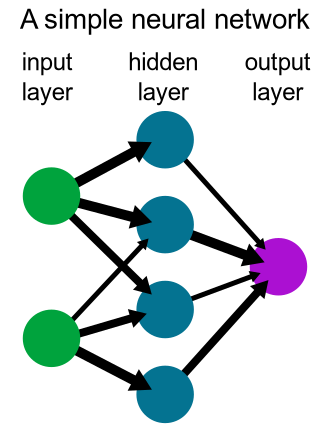
\includegraphics[scale=0.3]{background/neural_network.png}
	\caption{Neural Network image from Wikipedia, the free Encyclopedia}
	\label{fig:nn}
\end{figure}

\subsection{Deep Learning}
Deep Learning (DL) is a subset of Machine Learning that focuses on NNs with many layers. A conventional NN would only have 1 hidden layer whereas a DL network could go into the 10s or 100s (or more!). This is to accommodate ever-increasing dataset sizes. In the modern age, the sheer increase in data and parameters associated with ML is getting so large that certain problems require DL networks to solve them. This is so that every minute feature and detail can be extracted from the datasets and be properly represented by the model \cite{deeplearningbook}.\\ \\
They also include the use of activation functions between the layers. An activation function creates an output based on the output of the previous layer by applying a non-linear function to change it. Some of the most common to use are the $\tanh$ function and Rectified Linear Unit (ReLU \cite{relu}). We show some examples in \ref{tbl:activation-tbl}. \\ \\
For constructing DL models we will need to use some combination of these activation functions (and potentially others not mentioned \cite{wiki:activation}).

\newcommand{\tanhFunc}{
    $\tanh(x) = \dfrac{e^x - e^{-x}}{e^x + e^{-x}}$
}
\newcommand{\ReluFunc}{
    $ReLU(x) =
    \begin{cases}
      0 \hspace{0.5cm} $if $ x \leq 0\\    
      x \hspace{0.5cm} $if $ x > 0
    \end{cases}
    $
}
\newcommand{\SigmoidFunc}{
    $\sigma(x) = \dfrac{1}{1 + e^{-x}}$
}

\newcommand{\tanhDerivative}{
    $1 - \tanh(x)^2$
}
\newcommand{\ReluDerivative}{
    $
    \begin{cases}
      0 \hspace{0.5cm} $if $ x < 0\\
      1 \hspace{0.5cm} $if $ x > 0\\
      undefined \hspace{0.5cm} $if $ x == 0
    \end{cases}
    $
}
\newcommand{\SigmoidDerivative}{
    $\sigma(x)(1 - \sigma(x))$
}

\pgfplotsset{width=3.3cm,compat=1.9}
\newcommand{\sigmoidGraph}{
\begin{tikzpicture}
    \begin{axis}[xticklabels={,,}]
    \addplot[color=red]{1/(1 + exp(-x)};
    \end{axis}
\end{tikzpicture}
}
\newcommand{\tanhGraph}{
\begin{tikzpicture}
    \begin{axis}[xticklabels={,,}]
    \addplot[color=red]{(exp(x) - exp(-x))/(exp(x) + exp(-x))};
    \end{axis}
\end{tikzpicture}
}
\newcommand{\reluGraph}{
\begin{tikzpicture}
    \begin{axis}[
        domain=-3:5,
        xticklabels={,,},
        ]
        \addplot+[mark=none,red,domain=-3:0] {0};
        \addplot+[mark=none,red,domain=0:5] {x};
    \end{axis}
\end{tikzpicture}
}

\begin{center}
    \begin{longtable}{ | m{3.5em} | m{12.3em} | m{10.9em} | m{5.6em} | }
    \caption{Activation Function Table}
    \label{tbl:activation-tbl}
    \hline
    \textbf{Name} & \textbf{Function} & \textbf{Derivative} & \textbf{Example} \ \\ \hline
    tanh & \tanhFunc & \tanhDerivative & \tanhGraph \ \\ \hline
    ReLU & \ReluFunc & \ReluDerivative & \reluGraph \ \\ \hline
    Sigmoid & \SigmoidFunc & \SigmoidDerivative & \sigmoidGraph \ \\ \hline
    \end{longtable}
\end{center}

How these activation functions are used and when they are used can have an effect on the performance of a NN. Even fine-tuning certain combinations of activation functions can greatly improve performance \cite{activation_combined}.

\subsection{Convolutional Neural Networks}
DL models can be used for a variety of tasks but one that is quite common is that of image recognition. The popular structure for specific types of DL networks that focus on this is that of Convolutional Neural Networks (CNN). While typical NNs struggle in the complexity and detail of images, CNNs are more able to ``successfully capture the Spatial and Temporal dependencies in an image through the application of relevant filters" \cite{eli5_convnet}. The number of layers could in theory be increased but that adds vast computational power and it could lead to the over-fitting of the network. \\ \\
Instead we go for different architecture that consists of three distinct types of layers \cite{convnet}:
\begin{enumerate}
    \item \textbf{Convolutional Layer:} this layer takes a predefined kernel \cite{kernel} and applies it to the 2D image. If the input has more than one channel (e.g. an RGB image), then it is applied to each channel. The kernel that is used can change which features are highlighted and extracted depending on the use case. Some common kernels in Computer Vision are blurring kernels and Sobel kernels.The size of the kernel and how much it strides by in each step can decide as to how much reduction in dimensions there are.
    
    \item \textbf{Pooling Layer:} this layer is used to help decrease the spatial size of the previously convolved feature. This can then in turn decreases the processing power required to process the data as the size of the dimensions can be greatly reduced. This can be quite destructive to the data and so 2 more common approaches are to use a 2x2 kernel with a stride of 2 or to use a 3x3 kernel with a stride of two. The latter allows for overlap of the pixels but a kernel size above 3x3 can result in greatly decreased performance. Pooling is used to help detect patterns in images that are usually far too big for smaller kernels to detect actual patterns.
    
    \item \textbf{Fully-Connected Layer:} this acts like a typical NN and will try and form scores for the relevant classes/predictions based while connected in the standard way of being connected to all the neurons of the previous layer.
\end{enumerate}
An example of how these layers come together and form a CNN is below:
\begin{figure}[htbp]
	\centering
    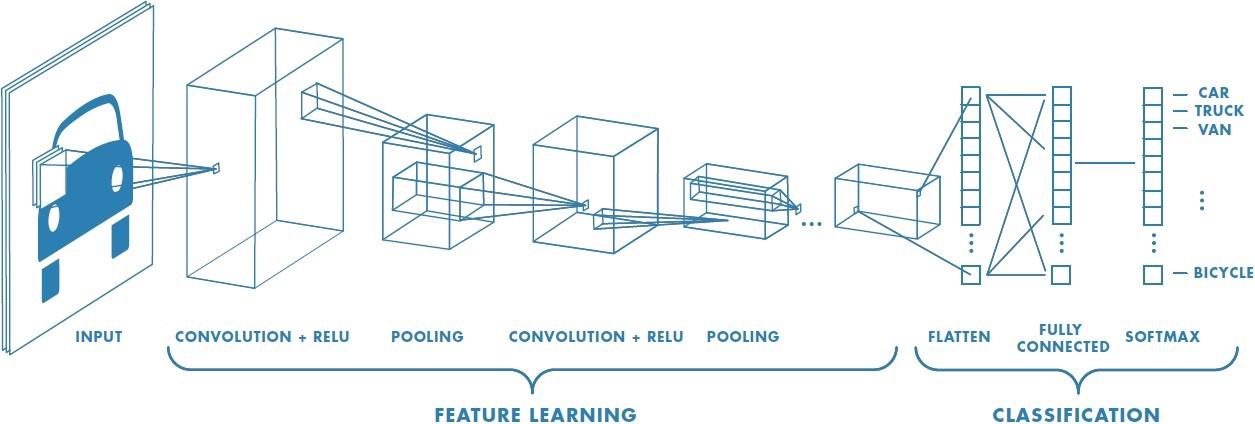
\includegraphics[scale=0.3]{background/cnn_example.jpeg}
    \caption{Visual Representation of CNN Layers \cite{eli5_convnet}}
    \label{fig:cnn-layers}
\end{figure}

For simple datasets like MNIST (where the dimensions of the images is only 28x28 and the image itself is fairly basic) we don't need a particularly complex NN beyond having the initial layer contain 784 (28x28) weights and so it doesn't necessarily benefit from a CNN. For something like the MedMNIST datasets, they are not in a higher dimension but are of higher complexity than that of standard MNIST and so more greatly benefit from the use of a CNN. Other examples of datasets that benefit this way are FashionMNIST \cite{fashion} and CIFAR-10 \cite{cifar}.\\ \\
One difference to note about the initial layer of a CNN compared to a standard NN is that it remains represented as a 2D array instead of being streamed into a 1D vector. This is something that allows the network to help recognise the patterns better as it retains the structure of the original image more precisely.



\section{Privacy Preserving Techniques}

With various methods of ML being applied to all manner of things to try and help make predictions about life better, it is only natural that the data in question will include personal data. Whether this is through monitoring app/website usage or very simply tracking what people ``like" or send to each other, the data is personal to each user and as such the experience of each user is personal. \\ \\
However, data can stray beyond this into more truly personal information such as that of the medical nature.
This is trickier to deal with, given that medical data is very tightly controlled and restricted due to its highly sensitive nature and the governing bodies controlling it are usually very unwilling to share. 
Now in the past this wasn't really an issue as typically only medical professionals of the governing organisation (e.g. the National Health Service (NHS)) would want access to this data and actually have any good reason. 
So it was very easy and efficient to deny any external access. 
However, we now live in a world where the prevalence of ML has made external researchers' access to data increasingly valuable to society. 
Users, beyond medical professionals, want access to this highly sensitive data to try and make the world a better place.
\\ \\
Whether this is in trying to train a model to recognise cancerous cells or early onset dementia, data surrounding that is needed to accurately make these predictions. 
So, to be able to push the field of medicine forward and to leverage to full power of modern day computing, we as software engineers need access to this data. 
So several methods of trying to preserve the privacy of the users of this data have been created to tackle this.

\subsection{Homomorphic Encryption}
Encrypting data seems to be a fairly intuitive starting point for trying to keep the privacy of user's data secured. 
For cloud computing \cite{cloud_fhe}, it is almost a necessity that the data is encrypted in some manner as otherwise employees of the company potentially have access to this data and could act maliciously \cite{access_private}. 
However, it results in a system where no one can read or understand the data without the appropriate decryption keys (usually not stored on a centralised server) and so trying to perform any calculations or processing on the data is somewhat redundant. 
So in comes the idea of Homomorphic Encryption. This is a style of encrypting data such that you are able to perform some given calculation on the encrypted data without the need for decrypting it first (e.g. addition).
\\ \\ 
However, only being able to perform 1 operation on the data isn't particularly useful and so the more impressive standard of Fully Homomorphic Encryption (FHE) was postulated \cite{fhe}. 
In theory, FHE allows for any number of operations to be performed (although current operations are typically just addition and multiplication) on the encrypted data. 
However, it is not a simple/intuitive system to implement for any given task and so for certain tasks, it may not be an ideal method on preserving the privacy of data.


\subsection{K-Anonymisation}
The idea behind anonymising data is to not be able to associate an individual person's data record with their actual identity in a given dataset. 
This helps to reassure that the data will not cause any worry or harm to that individual. This has the added side-effect of no longer making the data personal anymore and so more freely able to be used beyond the governing owner of that data. 
This is hugely beneficial to both parties and is a great starting point for preserving the privacy of the data. 
\\ \\
However, this is not as simple as it sounds and many attempts to pseudo-anonymise the data have resulted in people able to use more than one available dataset to link medical data with more available (and less sensitive) data like a voter list \cite{failed_anonymisation}.
\\ \\
Even if that weren't the case, you get certain attributes that when taken together are potentially able to identify a person. These are called quasi-identifiers. 
An example would be if you knew their post code and their date-of-birth, you could potentially figure out a disease they have if no one in that postcode shares that date-of-birth with them. e.g. id=3 in Table \ref{tbl:pre-anon}.
\\ \\
A way to tackle these is through the use of k-anonymising the data. A table of data is k-anonymous if every record in the table is indistinguishable from at least k-1 other records, with respect to every set of quasi-identifiers (not something that is itself a unique identifier, but when paired with other quasi-identifiers it can identify someone). 
The 2 styles of doing this are perturbative methods and non-perturbative methods but seeing as perturbative methods (e.g. adding noise) does not retain data integrity, we won't be considering it. 
Two main ways of achieving k-anonymity for non-perturbative methods are generalising the data (replacing attribute values with something more generalised e.g. 54321 $\longrightarrow$ 54***) and suppression (deletion of row or column e.g. row with id=3 in Table \ref{tbl:pre-anon}).
\begin{center}
    \begin{longtable}{ |c|c|c|c|c| }
    \caption{Pre-Anonymisation}
    \label{tbl:pre-anon}
    \hline
    \textbf{id} & \textbf{sex} & \textbf{DoB} & \textbf{postcode} & \textbf{disease} \ \\ \hline
    1 & female & 1998-03-13 & SW7 2BU & anxiety \ \\ \hline
    2 & female & 1998-10-27 & NW1 9LJ & anxiety \ \\ \hline
    3 & female & 1997-01-22 & AL9 7TA & chicken pox \ \\ \hline
    4 & male & 1999-11-11 & HP11 1UA & ADD \ \\ \hline
    5 & male & 1999-06-18 & HP14 4JQ & Dyspraxia \ \\ \hline
    6 & male & 1999-06-21 & HP11 2DQ & ADHD \ \\ \hline
    \end{longtable}
    
    \begin{longtable}{ |c|c|c|c|c| }
    \caption{2-Anonymised}
    \label{tbl:2-anon}
    \hline
    \textbf{id} & \textbf{sex} & \textbf{DoB} & \textbf{postcode} & \textbf{disease} \ \\ \hline
    \rowcolor{lightgray} 1 & female & 1998 & London & anxiety \ \\ \hline
    \rowcolor{lightgray} 2 & female & 1998 & London & anxiety \ \\ \hline
    \rowcolor{gray} 4 & male & 1999 & High Wycombe & ADD \ \\ \hline
    \rowcolor{gray} 5 & male & 1999 & High Wycombe & Dyspraxia \ \\ \hline
    \rowcolor{gray} 6 & male & 1999 & High Wycombe & ADHD \ \\ \hline
    \end{longtable}
\end{center}

The data is still susceptible to homogeneity and semantic attacks [Table \ref{tbl:2-anon}] and while {l-Diversity} can fix the former there is never any guarantee that a dataset is 100\% completely and truly anonymised. With k-anonymisation, a specific data record can't be identified with any given individual but information can still be inferred. The governing body behind the data sometimes has to make a decision about what is an acceptable level of anonymisation without completely destroying any utility or functionality behind it. There are some techniques being investigated through clustering of the data to help minimise information loss \cite{anon_cluster} but again, these only go so far. It should also be noted that k-anonymity can only work on table and record style data instead of things like images and so has its limitations there.


\subsection{Secure Multi-Party Computation}
A different approach for preserving privacy is when you have multiple parties all wanting to calculate something based on each others' data but no one wants to share their data. For this we have Secure Multi-Party Computation (MPC) and it is when 2 or more parties share their data with a 3rd trusted party and it carries out an algorithm that doesn't reveal anything about the parties' data that was given (unless the result of the function revealed the values anyway). \\ \\
However this involves a trusted 3rd party and so a different style would be through something called Secret Sharing (SS) and will be explained through the BGW Protocol \cite{bgw}. This expresses the function that is computed as an arithmetic circuit containing addition and multiplication gates. It involves the parties splitting up their value into ``shares" and sending them off to the other parties. Each party then calculates the function on those shares, broadcasts the output as new shares before combining the shares it receives into a value. This is shown in Figure \ref{fig:bgw}.
\begin{figure}[htbp]
	\centering
    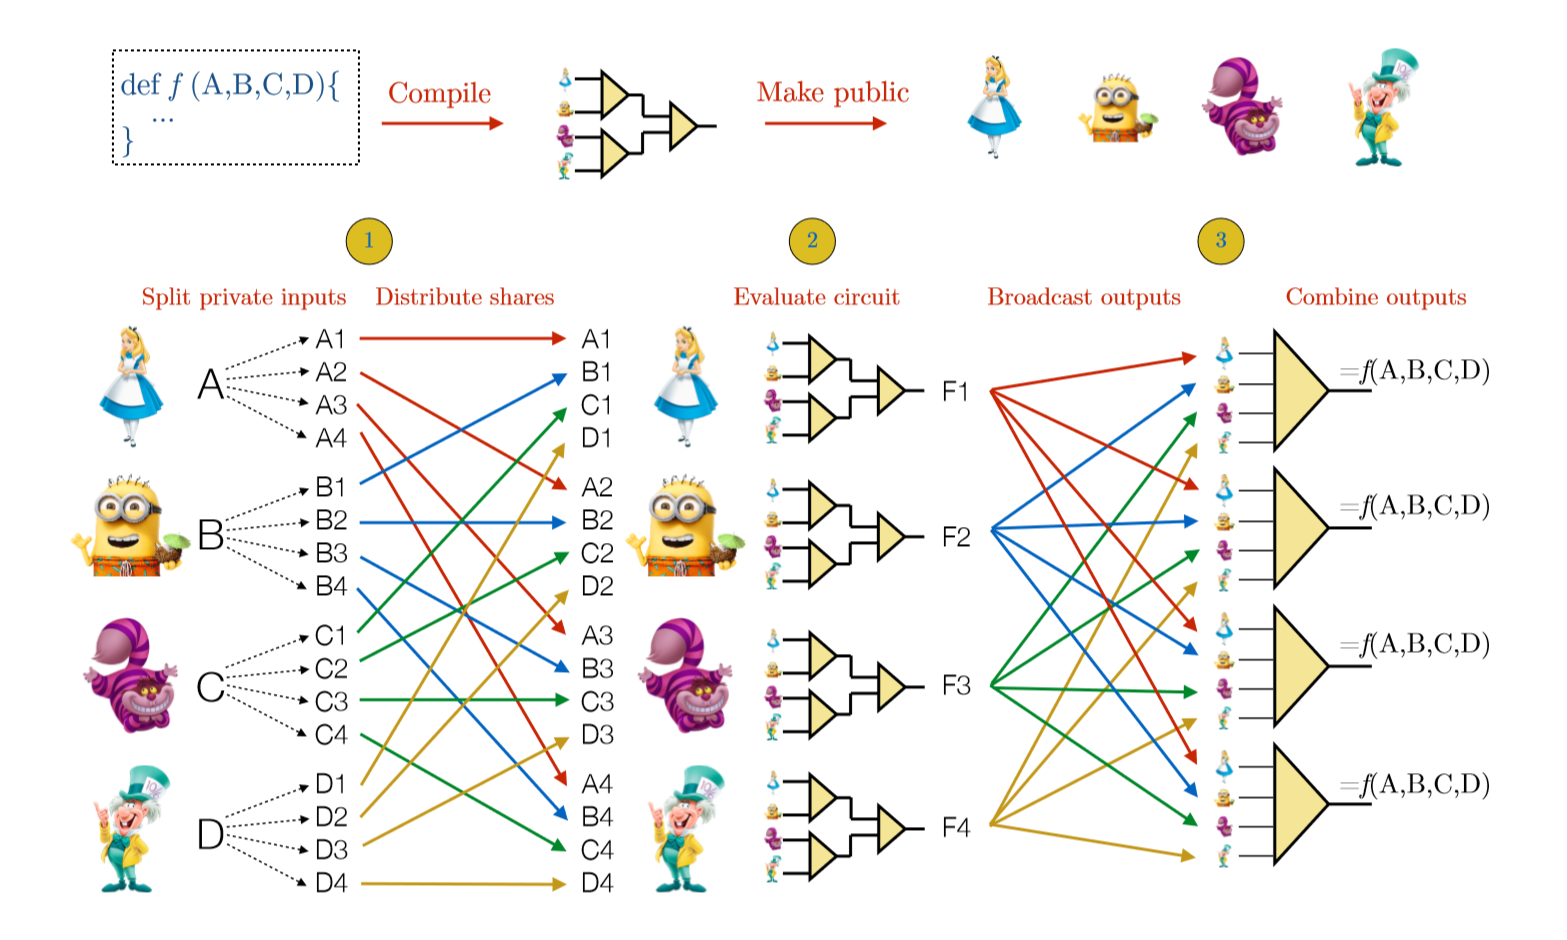
\includegraphics[scale=0.3]{background/bgw.png}
	\caption{BGW Protocol, courtesy of N. Dulay's Privacy Engineering Slides \cite{priv_eng}}
	\label{fig:bgw}
\end{figure}


\subsection{Differential Privacy}
Another method for preserving privacy is Differential Privacy (DP). DP guarantees that when you query a dataset D, the result that you get will be approximately the same (if not the same) irrespective of the presence of whether or not the dataset contained a certain value. This can be summarised as:
\begin{equation}
    Pr[x | y \in D] \approx Pr[x | y \notin D]
\end{equation}
As we want = instead of $\approx$ without destroying utility, we have the difference shown with $\epsilon$ such that:
\begin{equation}
    Pr[M(D) = y] \leq e^\epsilon Pr[M(D') = y]
\end{equation}
Where D is the dataset with no changes and D' is the dataset with the missing row. M is the function applied to D that computes the output and ensures privacy. We have to make sure that the two datasets satisfy the condition that they are neighbouring, i.e. they differ by exactly one row. This is what it means for a mechanism to be $\epsilon$-Differentially private. \\ \\
For achieving DP, the key ingredient is adding noise to the data until the above requirement is satisfied. This can be done with either Gaussian or Laplacian noise, with Laplace noise being the more common choice for DP. Typically, you draw from a Laplacian distribution that is $L(1/\epsilon)$ for the mechanism to remain $\epsilon$-Differentially private. Laplace's probability density function (pdf) is defined as:
\begin{equation}
    L(x|\mu,b) = \dfrac{1}{2b} \exp \left( -\dfrac{|x - \mu|}{b}\right)
\end{equation}

For ML models, depending on where we add the noise to, our mechanism will either be Locally or Globally differentially private. If the noise is added to the inputs of the model then it is Local DP. This involves each client adding noise so as to help protect their data. This helps ensure that each user has plausible deniability as you could never accurately claim that a certain client's specific data is of some specific value. If the noise is added to the end then it is Global DP. This is more desirable if the owner of the person taking the data and training with it is trustworthy as you can normally achieve more accurate results \cite{global_dp} as the input data has not been modified or changed. \\ \\
Interestingly, there are cases where adding noise to the gradient of models in very deep NNs \cite{dnn_noise} or as a form of regularisation for data augmentation \cite{robust_corrupt_noise} can help improve the generalisation performance of the trained model through either greater feature extraction ability or from reducing over-fitting.


\section{Federated Learning}

If data stayed amongst those that owned or governed it, then there would be less of a need for privacy preserving mechanisms. 
However in FL, while clients do process data on their own devices, the results are then sent to a centralised server for aggregation. 
\\ \\
In FL we are trying to have all the clients keep hold of their data whilst still being able to contribute it in a form that does not actually involve the sharing of it. The data is usually uneven as each client involved could have wildly different sizes of data or even wildly different backgrounds for the data. Two examples of this would be:
\begin{enumerate}
    \item Monitoring users' interactions with an app and training a model on the user's phone to make accurate predictions about what ads they'll like. 
    The model update calculated will be hyper-specific and over-fitted to an individual user at first. 
    But when you get 10s of 100s of users' models all being sent to a centralised server for aggregation, the model that will be sent back to each user will be much more generalised and better at making more accurate/clever predictions. 
    Through more rounds of back and forth it will eventually converge.
    
    \item If you had a group of hospitals that all had a large amount of patient data and they wanted to train a model for some arbitrary reason, they would be able to again train locally and send off the model just like before. 
    However, you could end up having 1 hospital that deals with a disproportionately large amount of elderly patients and their model would be skewed in that favour. 
    This can help the other hospitals who do not have as much access to such data. 
    This is a mutually beneficial exchange, as it also gives the original hospital more access to younger patient data. 
    As such, results are more easily able to generalise regardless of the age.
\end{enumerate}
As you can see, through FL, we are able to get more accurately trained models on otherwise private and sensitive data. 
This provides unprecedented potential for medical data to be used for research purposes where we will not need direct access to the data. However, as too-good-to-be-true as this might sound, there are obvious barriers in the way. 
For the hospitals and practices, not only will they have to standardise all of their data in an agreed-upon way, they will also have to hugely invest in some form of computing infrastructure such as something on-premise or in the cloud \cite{future_health_fl}. 
This involves a high initial cost as there is computing power needed for training such large amounts of data. 
This also does not mean that researchers outside of the hospital will even be able to use the data anyway, just that the Clinicians, Patients, Manufacturers and Healthcare providers can all benefit from the improvement of the ML-based systems \cite{future_health_fl}.

\subsection{Training}
The process of training the data for FL is as follows and is shown graphically in Figure \ref{fig:federated_learning}:
\begin{enumerate}
    \item Clients retrieve model from the central server.
    
    \item Each Client trains the model on its data and calculates a model update.
    
    \item Clients send the updates to the central server.
    
    \item Central server aggregates these updates together.
    
    \item Central server sends the new shared model back to the clients.
    
    \item Repeat 1-5 until convergence.
\end{enumerate}
\begin{figure}[htbp]
	\centering
    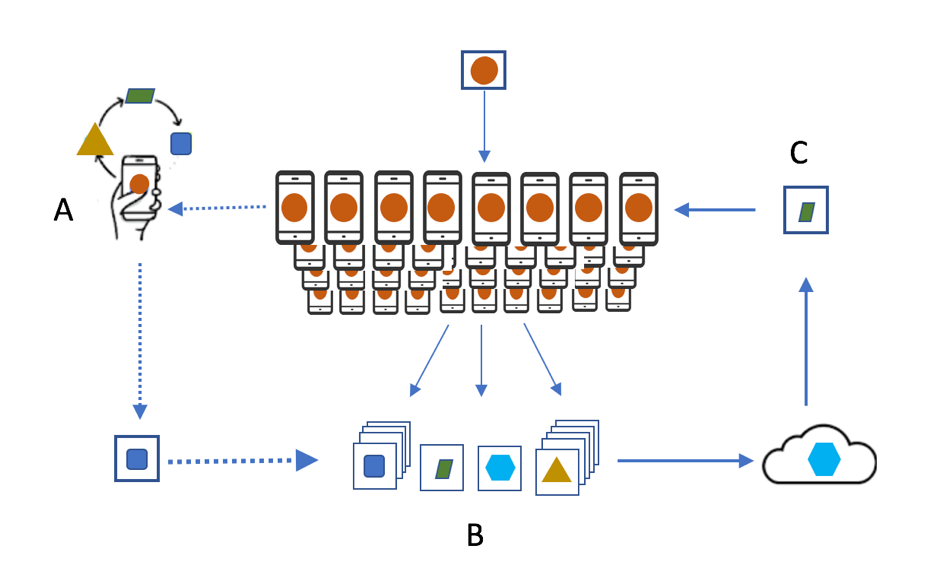
\includegraphics[scale=0.3]{background/federated_learning.png}
	\caption{Rough example of the exchange of ML models on user devices \cite{federated_learning}}
	\label{fig:federated_learning}
\end{figure}
The process by which the aggregation could be done is usually one of Federated Stochastic Gradient Descent (FedSGD) \cite{fedsgd} or Federated Averaging (FedAvg) \cite{fedavg}.
FedSGD aggregates on the models' gradients whereas FedAvg aggregates on the models' weights/parameters. \\ \\
In comparison to a baseline model with no FL employed, close to the exact same results can be achieved with standard FL with between a 0.008 and 0.014 Area under the Curve (AUC) difference \cite{babu}.


\subsection{Personalised Federated Learning}
Through this typical process of training, every client receives the same global model that has been aggregated through a contribution from everyone in some way, shape or form.
However, this might end up not being the most ideal strategy for achieving the best accuracy globally and locally.
Especially when it comes to non-independent and identically distributed (iid) data, being able to adapt the models that are sent out could be crucial for getting good performance.
\\ \\
One style in which this can be done is with Federated First Order Model Optimisation (FedFomo) \cite{fedfomo}.
Here, the method involves each client having a goal that it aims for that is based on its own validation and test data.
The central server then tries to group clients that want to achieve similar goals together so that they can contribute towards their own model together.
\\ \\
This method is a tad odd in that it does not seem to focus on generalisation and making sure the models utilise all of the data from the clients in a constructive way.
However, there are a variety of different ways in which this personalisation could be implemented and ultimately the solution chosen should reflect the problem that is trying to be solved.


\subsection{Privacy Amplification}
Attempting to amplify privacy via user sampling is a method in which not all clients are chosen to participate at every federated round.
Its main use is for helping to preserve the privacy of the clients involved through minimising honest-but-curious clients' interest in information leakage.
\\ \\
This seems like it would be an interesting solution to help the clients' privacy but unfortunately it is not without its drawbacks.
Experiments have shown that generally decreasing the probability (p) for clients to be picked leads to quite a significant decrease in convergence rate as well as a decrease in training accuracy \cite{privamp}.
\\ \\
Depending on what trade-offs you are willing to make, its gives the user quite a bit of flexibility in terms of having either more privacy, better accuracy or some combination of both.



\subsection{Possible Attacks}
Aggregating on the model updates from distributed clients seems to be a great strategy for accessing private data without it being leaked out. 
However, as all things that involve a human element, it can be exploited. 
The two main types of attacks are targeted and untargeted attacks.
Targeted attacks focus on the attacker trying to get the model to predict a specific thing incorrectly, e.g. telling an MNIST dataset that 5 is actually 7 to the extent that the global model starts classifying it as such. 
Untargeted attacks are just when the attacker tries to get the model to not reach convergence or a good accuracy.
\\ \\
Some different styles of poisoning (changing something in a negative manner) are highlighted in Table \ref{tbl:poisoning}. 
All methods excluding the final option are easily accessible to any client.
This is because the client owns their data and as such is in full control and can change it as needed. 
In terms of model reading and writing, the client will receive the model and can send back whatever they like. 
The central server has no way of stopping any of this and without breaking the whole notion behind federated learning, cannot have the clients data checked for tampering (unless some encrypted form of ML was used, which is extremely slow and computationally expensive). \\ \\
In theory if you had control of the client side as well (e.g. a mobile app), then you probably would not need to worry about the model poisoning side of things. 
The final option assumes that the malicious client essentially has complete control over the system and at this point it is essentially impossible to design a robust aggregation system \cite{robagg_fl}.
\begin{center}
    \begin{longtable}{ |c|c|c|c|c| }
    \caption{Poisoning Attacks \& Corruption Examples \cite{robagg_fl} - \textbf{Data Write} is changing of data in dataset, \textbf{Model Read} executing code based on model update before update takes place, \textbf{Model Write} is running code instead of standard update code and \textbf{Aggregation} is running code instead of the standard aggregation function on the central server}
    \label{tbl:poisoning}
    \hline
    \textbf{Corruption Type} & \textbf{Data Write} & \textbf{Model Read} & \textbf{Model Write} & \textbf{Aggregation} \ \\ \hline
    None & - & - & - & - \ \\ \hline
    Static Data Poisoning & Yes & - & - & - \ \\ \hline
    Adaptive Data Poisoning & Yes & Yes & - & - \ \\ \hline
    Update Poisoning & Yes & Yes & Yes & - \ \\ \hline
    Byzantine & Yes & Yes & Yes & Yes \ \\ \hline
    \end{longtable}
\end{center}
There's also the case to handle where it may look like an attacker is trying to cause damage when it actuality it's just a faulty client. 
Depending on the level of damage done it may be beneficial to actually not block faulty clients, as they may introduce noise that improves the model's generalisability \cite{dnn_noise, robust_corrupt_noise}. 
However, you are most likely going to end up blocking them as they could be damaging your performance without themselves realising it.

\subsubsection{Data Poisoning}
This involves maliciously changing the data in an attack. 
It could be done by adding noise or changing labels but as long as the original dataset has been changed, it is considered as having undergone a data poisoning attack. 
It has been shown that data poisoning attacks have been able to achieve a high-confidence of misclassification for deep NN \cite{poison_dnn}. 
\\ \\
There is also a difference between static and adaptive data poisoning. 
Static is where the data is poisoned once at the beginning (prior to training). 
Adaptive is seeing how the models change and then change the data at the beginning of each round so as to accommodate for it. 
Adaptive is more complex but could have the potential to achieve better results as the attack ends up being more tailored.

\subsubsection{Model Poisoning}
This technique uses the model to help craft a specially designed model update. 
In the targeted case, we would have a goal for misclassification but with all of the other users averaging out the poisoning, we would need to change the update in such a way as to negate the combined effects of the benign clients.
Evaluation done has shown that this can lead to 100\% confidence in target misclassification while also impressively achieving convergence of the model \cite{adversarial_lens}. 
\\ \\
To help avoid detection (if the aggregation done is attempting to be robust) where the central server has stealth metrics to identify malicious clients, the malicious objective can be modified so as to account for these detections. 
With this you can normally go undetected for the majority of the rounds but a more clever strategy where we use ``alternating minimisation" to account for both stealth and model poisoning so as to help go undetected for all of the rounds \cite{adversarial_lens}. 
The aim is to minimise for the adversarial objective first and then minimise for the stealth objective for any given epoch.

\subsubsection{Free-Riding}
Attacks do not necessarily come in the form of trying to manipulate the model in a negative way. 
One method involves ``Free-Riding" \cite{free_riding} where the client instead has a goal of trying to gain the completed model without actually contributing anything to the cumulative effort. 
This might be done when the models have commercial/intellectual value and can subsequently lead to intellectual property/financial loss. 
The client would have to trick the rest of the clients into thinking that they have useful and valuable data to contribute.
The size at which the free-rider decides to claim their data is up to them, but is typically the average of the rest of the data.
\\ \\
The initial way of doing this would be to simply return the model's parameters at each round. 
However, this can easily be checked for by the central server.
The way to get around this is to add some Gaussian white noise to the parameters and gradients that is of a similar structure to the benign clients' responses.
This is done by monitoring the mean and variance of the other responses and adjusting accordingly at each round.
The main effect adding noise has is that the resulting variance of the accuracy will increase and the amount it increases is dependant on the variance used by the free-rider.
However, it should be noted that the increase in variance did not appear to show a significant increase in loss and so it could be considered worth it for the anonymity.
\\ \\
However, the noise variation that is typically observed by the benign clients, through something like SGD, decreases as the model converges.
So the free-rider must in turn decrease their noise in a similar asymptotic manner to their noise added.
This again works until a certain extent but anomaly detection methods such as Deep Autoencoding Gaussian Mixture Models (DAGMM) \cite{dagmm} have been shown to detect the free-riders as anomalies \cite{freerider_defence}.
\\ \\
The main way for free-riding clients to then hide is to use a ``delta-weight attack" \cite{freerider_defence}.
Here, they instead use the difference between the previous and current global models and assign that difference to the gradient weights of the parameters.
This emulates the average gradient weights from all of the other clients and so becomes a very neutral client and so can avoid detection much better.
Wonderfully, with the use of privacy amplification, it becomes easier for the central server to detect these delta-weight attacks.
This is because they are only getting model updates every few rounds when selected and so their model that they contribute has gradients with far more eccentric changes than they would otherwise have.
\\ \\
``This result is in agreement with our theory, for which the convergence speed is inversely proportional to the relative size of the free-riders" \cite{free_riding}. 
However, it should be noted that too many free-riders will detriment the global model to some extent and so these attackers should be wary of the effect that they have.
This becomes slightly less of a problem with DP as the inherent added noise almost mimics that of a free-rider and so there is more expectation of fluctuations of accuracy.
It also allows the free-riders to hide themselves better amongst the other clients, which is a nice added bonus for them.
\\ \\
The nature of free-riding becomes quite an elusive game of cat-and-mouse with ever increasing concealing and detection.
It's quite a wondrous area for further investigation and implementation testing.





\section{Non-Robust Aggregation}

When it comes to aggregation, there are a variety of different methods which people have tried so as to achieve different results.
This can vary from using encrypted data, simple weighted-averaging of data or more robust methods.
When it comes to non-robust strategies, the typical focus is on trying to make the accuracy as good as possible and ideally with non-iid data.


\subsection{FedSGD}
FedSGD is based on the idea that you would sample the gradients of the model from each client and then have them all averaged proportionally based on the number of samples of each client.
The update strategy is simply that of SGD:
\begin{equation}
    \omega_j = \omega_j - \alpha \dfrac{\delta E_i}{\delta \omega_j}
\end{equation}
Where E is the error function (typically $L^2$ norm or cross-entropy) and w is the parameter that's being updated.
\\ \\
It sometimes also involves a selective parameter update, where only a certain number of the parameters are chosen each round.
This can be done at random but a smarter way is to use the models that have the largest gradient change and so in theory will contribute the most to the global model.


\subsection{FedAvg}
FedAvg was made to improve on FedSGD by instead focusing on the model weights instead of the model gradients \cite[section 2.1]{robagg_health}.
This has been shown to be an improvement on using the gradients and is typically used in other modern aggregation tasks.
It can be described through the formula:
\begin{equation}
    \theta_g = \mathlarger{\mathlarger{\sum}}_{i=0}^{\infty} \dfrac{d_i}{d} \theta_i
\end{equation}
Where $d$ denotes the entire dataset size, $d_i$ is the size of the dataset for model i and theta is the model parameter.


\subsection{Federated Matched Averaging}
Federated Matched Averaging (FedMA) \cite{fedma} was brought about to solve federated learning accuracy problems that occur in modern architectures and models such as LSTMs and CNNs.
Due to their deep and more complex nature, these architectures do not aggregate well under more coordinated style aggregations, like those found in FedAvg.
\\ \\
The algorithm works by aggregating the models layer-by-layer by starting with the initial layer and performing a weighted-averaging on it.
It then proceeds to broadcast this layer out to the clients and the clients then continue to train all of the layers after the broadcasted layer for a few rounds.
The aggregation then happens for the second layer and the process is repeated until the last layer.
Now, the number of times communication is required is equivalent to the number of layers and not a more arbitrary hyper-parameter set by the central server.
In theory, FedMA is then supposed to have far fewer number of communication rounds compared to FedAvg while out-performing it.
Experiments show \cite{fedma} that FedMA is capable of out-performing all other aggregation methods in accuracy across a variety of datasets that use more complex architectures.


\subsection{Auto-FedAvg}
Auto-FedAvg \cite{autofa} was born out of the need to handle non-iid data, whilst still improving overall accuracy.
Instead of having the weights for the weighted-averaging of the aggregation be fixed, they become learnable parameters that can adapt as the aggregation rounds occur.
\\ \\
In this algorithm there are two sets of weights: $\alpha$ and $\beta$.
$\alpha$ contains the set of learnable weights that the central server uses for aggregation and $\beta$ is what $\alpha$ is parameterised by during the learning process through an activation function $\gamma$.
In this case $\gamma$ can either be the Softmax function or a Dirichlet distribution where $\alpha$ is the set of random variables with concentration $\beta$. 
Dirichlet is as follows:
\begin{equation}
    Dir(\alpha | \beta) = \dfrac{1}{B(\beta)} \mathlarger{\mathlarger{\prod}}_{k=1}^{K} \alpha_k^{\beta_k-1}
\end{equation}
where $B(\beta) = \frac{\prod_{k=1}^K \Gamma(\beta_k)}{\Gamma (\sum_{k=1}^K \beta_k)}$ and $\Gamma(z) = \Sigma_0^\infty x^{z-1} e^{-x} dx$ is the gamma function.
\\ \\
Each round, the clients sample a mini-batch of their data and compute the $\alpha$ before using these weights in the aggregation.
The loss of the $\beta$ weights is then calculated with regards to the mini-batched data before $\beta$ is subsequently updated with $\gamma$.
The server then gathers up each $\beta$ weights from each client's local loss calculation and they are averaged to form the $\beta$ for the next round that is used to calculate the $\alpha$.
\\ \\
\textit{N.B. the paper relating to this method \cite{autofa} was released in April of 2021 and is still under development. As such, the methodology and implementation is still up to change as well as their experimentation results. In this area, it claims to be SotA and that it is better than FedMA in similar tasks, but this has not been peer-reviewed as of writing.}


\section{Robust Aggregation}

Unfortunately, having a raw aggregation method is suspect to a variety of potential attacks from any number of malicious users. 
In some cases, it might take a single client to have the model predict inaccurately. 
As such, we have to look outside non-robust aggregation methods like FedSGD and FedAvg. 
This can typically involve not including the malicious clients in the aggregation, giving the malicious clients a lower weighting in the aggregation and/or just completely blocking the clients once a certain threshold is met. 
\\ \\
Any of these methods have their cons in that it is possible in all cases to end up blocking at least one of the benign clients as well. 
When the number of clients is small this can have a much more detrimental affect due to a significant chunk of the training data is lost. 
Increasing the number of clients would mitigate the effect of this but there is still an issue of have the benign clients' data lost. 
A couple of different methods for robust aggregation will be introduced along with their performance under different styles of attacks.

\subsection{Krum}
To tolerate $f$ byzantine clients (malicious/faulty) out of a total of $n$ clients, Krum \cite{krum} achieves its byzantine-resilience property by looking at every subset of $n-f-1$ clients. 
It goes through each client and calculates the sum of the squared-distances between the client and their closest $n-f-2$ neighbours.
This becomes the score of that client and Krum takes the client with the best score and uses a data sample from that client.
With this method, Krum is able to theoretically tolerate up to f byzantine clients under the condition of $2f + 2 < n$. 
\\ \\
Another development on Krum brings in the idea of averaging to it, called Multi-Krum (MKRUM).
You take the top scoring $n-f$ clients' parameter vectors and average them together so as to be able to better leverage multiple correct (or at least correct by KRUM standards) clients.
This helps to reduce waste and not to throw away data. However, MKRUM still (and even more so Krum) throws away a lot of clients' data that might be useful. It also takes on a position where $f$ might not be chosen correctly, leading to even more data unnecessarily being thrown away.

\subsection{Coordinate-wise Median}
A simpler approach to choosing an individual client's parameters is through Coordinate-wise Median (COMED) \cite{comed}.
For all parameter vectors from all of the clients, COMED takes the median value of each of the parameters throughout all of the models.
This is defined mathematically as:
\begin{equation}
    g_k = med\{x_k^i: i \in [m]\}
\end{equation}
where k is the k-th parameter and m is the number of clients involved.
This very nicely gets to utilise all of the clients to try to have as balanced of a choice as possible for all of the model parameters.
It also performs quite well, generally better than MKRUM in an adversarial test while being a bit more sensitive to noise without any bad clients involved \cite{robagg_health}.

\subsection{Adaptive Federated Averaging}
A different way to handle byzantine clients is to simply block them, as done by Adaptive Federated Averaging (AFA) \cite{afa}.
It determines if a client is malicious based on the cosine similarity ($s_k$) between the model updates from the clients and the global aggregated model's parameters.
With this it also adaptively assigns weights to the clients for aggregation.
\\ \\
Assuming that the number of byzantine clients is less than half of the total clients, we use the median ($\hat{\mu}_s$), mean ($\bar{\mu}_s$) and standard deviation ($\sigma_s$) of the similarities of the clients. AFA works as $\hat{\mu}_s$ must be one of the good values due to the the number of byzantine clients being less than half. We then make two comparisons for determining if a client is bad:
\begin{equation}
    \begin{cases}
      \hat{\mu}_s < \bar{\mu}_s \longrightarrow s_k < \bar{\mu}_s - \xi \sigma_s\\
      \hat{\mu}_s \geq \bar{\mu}_s \longrightarrow s_k < \bar{\mu}_s + \xi \sigma_s\\
    \end{cases}
\end{equation}

If either of these constraints is met, then the client is deemed to have sent a bad update and so is blocked.
This strategy for robust aggregation is also shown to consistently outperform previous methods on certain datasets \cite{robagg_health}.

\subsection{FedMGDA+}
Another method involving the blocking of clients is FedMGDA+ \cite{fedmgda}. 
This takes a subset of clients and for each one, performs a client update.
This involves a single layer NN that aims to minimise the loss.
For each client, the input to the NN is the difference between the client's model and the global model.
The new weights for the clients are then returned and used for aggregation.
The central server then aims to learn the relevance of each client based on the importance assigned to it. 
This importance is initially chosen based on dataset size of the respective client.
Malicious clients are hopefully deemed less important until they reach a certain threshold and are then subsequently blocked.
\\ \\
The performance of FedMGDA+ really shines through when comparing its performance with and without attacks \cite{fedmgda}.
For no attacks, it tends to perform a bit worse on average compared to other aggregation methods like FedAvg.
However, when attacks are introduced, it performs much better than certain other aggregators due to its dynamic weighting system in place.

\subsection{Group-wise Robust Aggregation}
A different approach is to try and minimise the variance of model parameters so that we can improve the resiliency of the aggregation.
One technique of doing this is through group-wise robust aggregation (GroupRA) \cite{cluster_robagg}.
Here the model parameters from the clients are clustered based on similarity (e.g. difference between parameter values).
A popular choice would be k-means clustering. 
While this has some extra overhead of trying to find the optimal k, it is still manageable to find through trial and error.
We can then apply aggregation to each cluster individually using any aggregation of choice (e.g. FedAvg, FedSGD).
\\ \\
Clustering gives byzantine clients 2 options, to be spread out or for them to try to stick together and actively deviate the centre of the cluster.
\begin{enumerate}
    \item Here the clusters can be made smaller, essentially relying on the robust aggregation to eliminate the byzantine clients
    
    \item Here the byzantine clusters can collectively try and make their cluster be moved towards their ideal target.
    This somewhat falls down due to the majority of clusters being benign.
    So when the cluster centres are used for the global model aggregation, the weighting of the scoring function helps minimise the deviation introduced.
\end{enumerate}
\\ \\
We then need to decide on a method of scoring.
A typical choice would be to have each cluster weighted by its normalised cluster size.
A more refined method would be to take the single cluster centre for each cluster and apply that to the global model and test it on a small dataset.
Weights are then assigned based on their accuracy but it could be quite a computationally expensive process.
\\ \\
When tested under a small model poisoning attack with CIFAR-10 and MNIST, GroupRA achieved a higher accuracy than the other robust aggregation strategies tested (e.g. KRUM). 
It should be noted though that there were some k-means clustering optimisation going on here as well.
Unoptimised k values end up performing just as badly as the other aggregation methods.
This is because with too few or too many clusters, we revert back to the standard robust aggregation method.

\subsection{Spectral Anomaly Detection \& Variational Auto-encoder}
Spectral Anomaly Detection (SAD) is a highly effective anomaly detection method \cite{sad}.
The data is embedded into a low-dimensional state regardless of if it's benign or not.
Through looking at reconstruction errors and learning to remove noisy features, you should easily be able to identify abnormal instances \cite{variationalAB}.
\\ \\
Through the use of an encoder-decoder architecture \cite{spectral}, you can train it to recognise byzantine clients as they trigger a higher reconstruction error.
The encoder takes the original data and does the SAD to output the low-dimensional embeddings.
The decoder then creates a reconstruction error from these embeddings and uses that error to optimise the parameters of the encoder-decoder model until convergence.
\\ \\
For the encoder, a Variational Auto-Encoder (VAE) is used with dynamic thresholding.
This has benefits over other methods as the detection threshold is only created after the central server has received all of the clients' model updates.
This stops the byzantine clients from knowing the detection mechanism beforehand, which can help with them not being able to carry out more clever model-poisoning attacks to escape being caught.
\\ \\
This works as the byzantine clients have to make quite significant changes for their model update to have any real effect.
This is due to the averaging nature of the base aggregation of FedAvg or FedSGD.
So these larger updates become more noticeable under the scope of the encoder-decoder model due to the size of the reconstruction error.
\\ \\
The ways in which other aggregation methods can fail where SAD VAE doesn't are:
\begin{enumerate}
    \item Hard-Thresholding (Sign-Flipping): the VAE uses dynamic thresholding at each round after receiving the model updates and so isn't susceptible.
    
    \item Noise: adding some noise to the model can help protect privacy through DP but when too much is added it can hurt the model's accuracy. 
    The SAD helps negate this somewhat by having the step to reduce noisy features so as to focus on the more import features of the data.
    
    \item Model Poisoning: this requires prior knowledge of the system and seeing as the VAE is dynamic, trying to use crafted smaller updates to not get picked up won't work as well here.
\end{enumerate}
Through experiments done \cite{spectral}, it has been show that the model accuracy with attacks can come closer or be the same as model accuracy without attacks.


















%mention https://arxiv.org/pdf/1911.00222.pdf as in DP before rob agg



%%%%%%%%%%%%%%%%%%%%%%%%%%%%%%%%%%%%
\chapter{Robust Aggregation}
To find a baseline to build upon, we conduct some investigations into the current best methods of Robust Aggregation.
However, aggregators like MKRUM, COMED and FedAvg don't have much complexity to them and as such don't have parameters that can be tuned.
We look into several categories for initial testing such as AFA, FedMGDA+ and aggregator limitations. 
AFA and FedMGDA+ are especially promising in their ability to block faulty/malicious clients. 
It is also important to check how the the local rounds affect detectibility of these bad clients.
\\ \\
Faulty Clients: 1, 3, 5, 7, 9, 11, 13, 15 17, 19
\\
Malicious Client: 2, 4, 6, 8, 10, 12, 14, 16, 18, 20
\\
Mixed: first 5 of each.
\\
The weighting given to each client as to how much data they get varies from about 2-4\% and is hard-coded in.
\\ \\
One thing to note is that the faulty clients are very faulty in this setup, more broken than just noisy.
This is because just slightly noisy clients can actually benefit the robustness of a model. 
Thus, they are not considered harmful or in need of being detected.

\section{AFA}
For this investigation we kept the local rounds at 10 epochs per round and used all three attacks.
Apart from just looking at the hyper-parameters of xi, deltaxi, aplha and beta, we also observe how many clients get blocked.
This is because one can have a very strict system that ends with good accuracy, but that also blocks a significant number of good clients.
This is not an ideal situation to be in and so should be avoided wherever possible.
We use IID data and are thus less affected, but in real-world situations missing data could have quite a performance impact on the model when testing.

\subsection{Parameters}
\begin{enumerate}
    \item Alpha: the numerator used in calculating the score of each client. Increments if the client doesn't give a bad update. Also used in blocking check via a beta cdf distribution.
    \item Beta: the denominator used in calculating the score of each client. Increments if the client gives a bad update. Also used in blocking check via a beta cdf distribution.
    \item Score: a value used for giving a model weighting in the overall model merging so that we know how much importance to assign each model.
    \item Xi: used as part of calculating whether or not a client should be classified as giving a bad update.
    \item DeltaXi: added the the xi every time there is at least 1 bad update, changing the threshold for being classified as a bad update.
\end{enumerate}
We try a range of xi from one-three, deltaXi from 0.25-0.75 and alpha \& beta from two-four.

\subsection{Results}
The results show:
\begin{enumerate}
    \item 10 malicious clients caused the model to fail in all tests such that it never learned anything regardless of the parameters. [\ref{fig:mal_afa}]
    \item Having a xi value above two causes the initial threshold to be too weak and as such never blocks any clients. This is further shown by when the xi was 2 and the deltaXi was set to 0.75 but to less effect [\ref{fig:afa_2_0.75}]. 
    However, the error rate did wobble and vary a bit between alpha/beta combos and so the model wasn't \textit{completely} destroyed, just not usable.
    \item Lower xi and deltaXi values consistently performed the best and acted more just like a non-federated solution.
\end{enumerate}

It may seem as if the solution is to use a low xi of one or two and a low deltaXi. 
However, we observe that xi values that performed the best and blocked all of the malicious/faulty clients, then proceeds to block a hearty amount of benign clients as well.
Around 9-11 of the benign clients get blocked at some point in the training when the xi is one.
\\ \\
This is bad for non-obvious reasons. 
In other aggregators, malicious/faulty clients simply don't get used or receive lower weightings. 
So even if you are a benign client that has some weird data, you can still contribute in some manner or at least aren't branded as bad. 
However, if a hospital gets blocked from contributing more data and isn't allowed access to the finalised model due to a faulty aggregation system, this could negatively impact its ability to provide quality healthcare.
\\ \\
Furthermore, blocking off clients with more unique data may end up harming your model as it only learns the most common data (which can be warped from an attack quite easily!). This is also true in non-IID scenarios.
\\ \\
So we want to find the mix between blocking as few benign clients as possible (ideally none) and blocking as many bad clients as possible (ideally all), while reducing the error rate.
Based on our tests, this leaves us with one option: a xi of two and a deltaXi of 0.25.
This does make sense as we don't want drastic changes each time and so having the delta small at 0.25 works well. 
This is further backed by the best alpha/beta to be both four [\ref{fig:best_afa}] as it then allows for smaller changes in division when calculating the score when the alpha/beta value gets changed.

\begin{figure}[htbp]
	\centering
    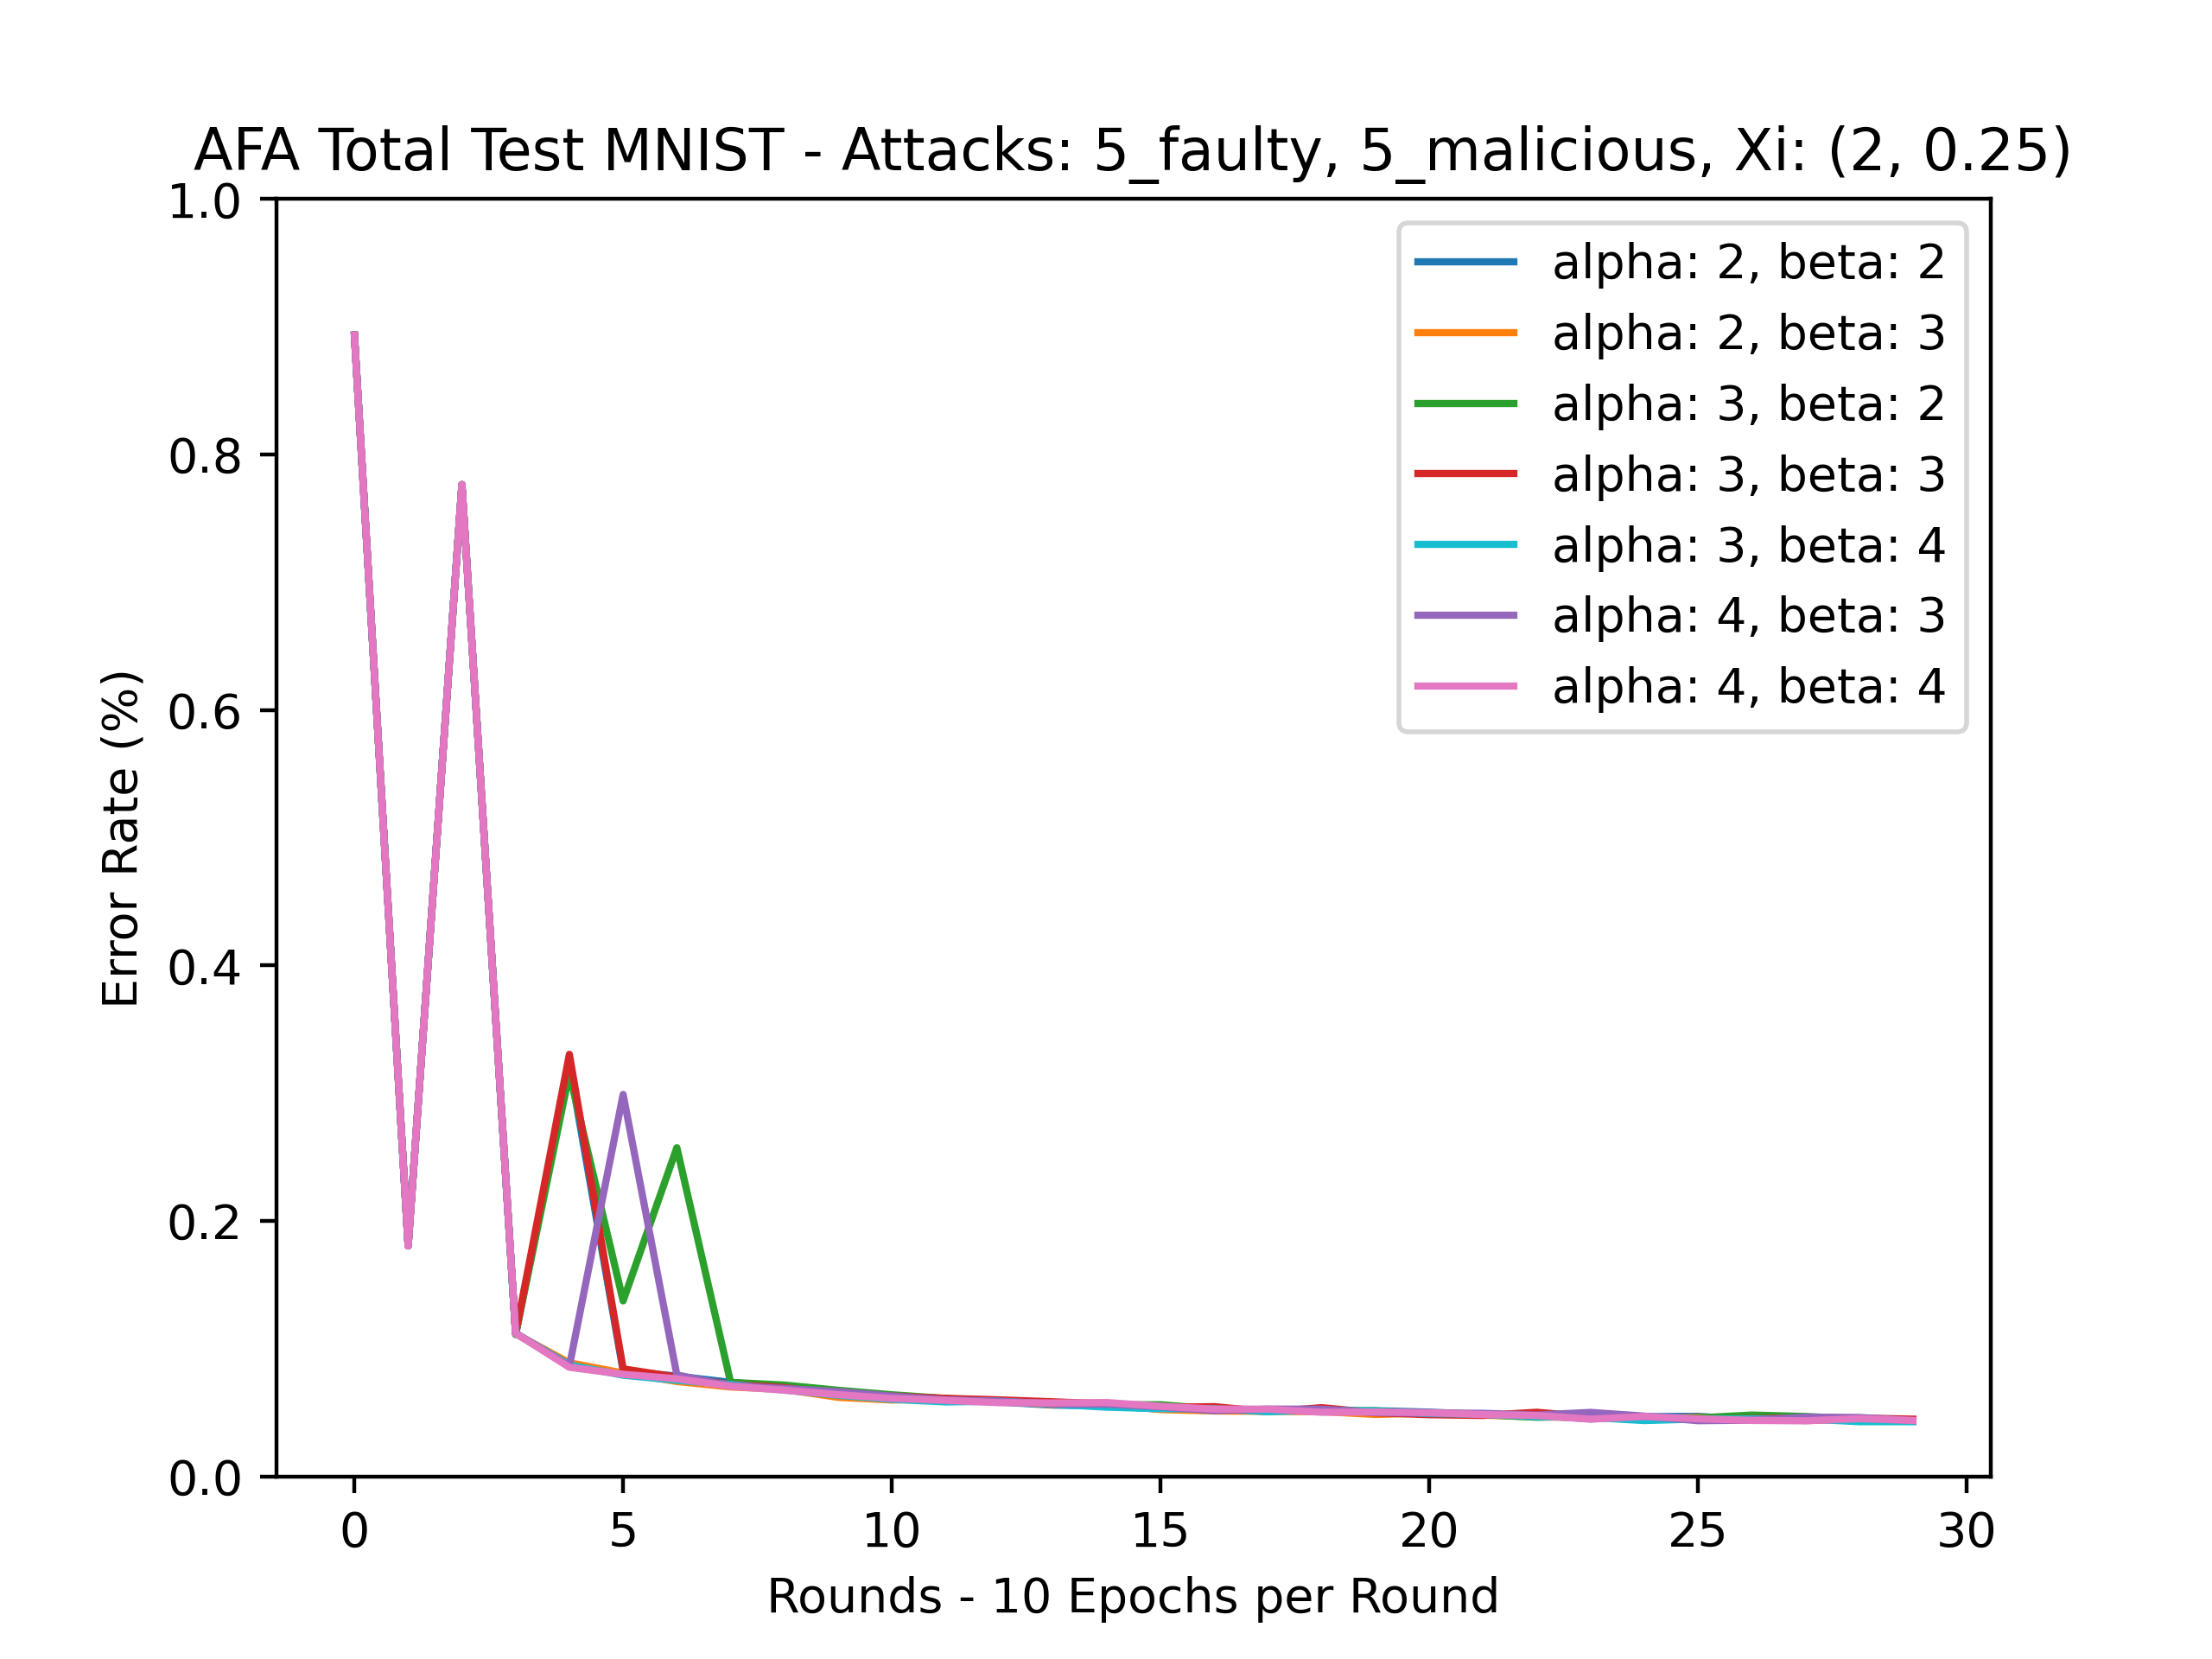
\includegraphics[scale=0.7]{initial/graphs/best_afa.png}
	\caption{AFA - Xi: 2, DeltaXi: 0.25}
	\label{fig:best_afa}
\end{figure}


\section{Improved FedMGDA+}
This investigation was very comprehensive and involved looking at the threshold used for blocking, the LR of the internal layer and the number of epochs per local round. 
Similar investigations were in place to make sure that not too many benign clients were getting blocked for the same reasons labelled above.
For this there were 50 federated rounds with a varying number of epochs per round.
\\ \\
It should be noted that we made significant fixes and improvements to the initial implementation, to ensure its correctness. Ensuring the stability of Improved FedMGDA+ formed a significant portion of our project.

\subsection{Threshold}
We decided to base the threshold on a factor inverse to the number of clients involved.
For example, with 30 clients I would try 1/60, 1/90, 1/3000 etc.
This was so that any arbitrary number of clients could join or participate, unlike with a hard coded threshold.
\\ \\
This ended up being quite a disappointing investigation as we had initially gone into this thinking that the weights we were checking against when deciding on blocking would get really small if the client was bad. 
However, all we saw happen is that when the model identified clients as bad, their weights very heavily just went into the negative.
This meant that no manner of threshold was going to have an impact as the weights would simply hop into the negative.
There were some \textit{slight} deviations as shown in [\ref{fig:mgda_var}].

\subsection{LR and Epochs}
These two are linked by their relationship; if you increase the number of local epochs per federated round, then overall there will be more rounds of learning going on. 
This also causes the local models to learn more about their own local data before aggregating together. 
This might mean that you might/might not want a higher LR to have the newer parameters taken more seriously.
\\ \\
Looking into the results it is really easy to get tricked and believe that the best option is to just crank up the LR and have at least six local epochs per round. 
This is because you get some great graphs that have the error rate quickly converge to a low result [\ref{fig:fake_good}].
It's noticeable that the LRs above 0.5 have essentially converged by round 10 to a good result.

\subsubsection{Hidden in the Grit}

Alas, just like with AFA, the real information comes out in the grit of which clients were blocked and when.
When you look at that, you see that all-bar-one benign client gets blocked in rounds one-three.
Funnily enough, over these three rounds is exactly when all of the malicious clients get blocked as well.
This pretty much leads me to believe that the malicious clients aren't getting blocked because they are actually being recognised as bad, but instead because the aggregator is deciding to block the clients en-mass.
It just so happens that the malicious ones are caught in the cross-fire of all of the mass blocking.
\\ \\
However, when we look at the lower end of the LR, we get much slower convergence but with absolutely no benign clients being blocked and all of the byzantine ones getting blocked.
This would be cause for celebration if it wasn't taking the aggregator 46 rounds out of 50 to actual do the blocking...
So, looking at lower numbers of epochs per round, we see that 1/2 looked like they work much better.
They showed a mix of being able to block all of the malicious clients [\ref{fig:1epoch_grid}] and achieving a good, low error rate [\ref{fig:2epoch_grid}] but not quite both.
These results tend to occur at around LRs of 0.01 to 0.05 and so further refinement needs to be done.

\subsubsection{Refinement Needed}
Looking into a more refined LR, we again notice that an epoch count of one produces results such that the malicious clients get blocked at great points such a round 16 or so but still don't converge to the ideal error rate.
However, two does not block early enough or ends up blocking some benign clients.
The latter ends up being quite an easy fix as these clients end up being blocked in around the 30\textsuperscript{th}-50\textsuperscript{th} round.
The solution is to reduce the number of rounds that the aggregator runs for.
\\ \\
Finding the balance between these two options proved to be fairly simple: an epoch count of one simply never showed a low enough error rate so two will be the best starting point.
In our project, we use an adaptive approach, and had the LR either increase or decrease as the rounds go on. 
While we could have tried many LR update methods, such as a sinusoidal LR or one that increases and decreases, finding an optimal method would have introduced runaway complexity. It was also beyond the scope of this project.
\\ \\ 
A decreasing LR from the values of [0.1, 0.09, 0.08, 0.07, 0.06, 0.05] to [0.05, 0.04, 0.03, 0.02, 0.01] in a linear fashion proved to be the best course of action.
This followed a fairly logical course of thought, such that you want to start out with a higher LR initially to help differentiate between the clients more.
Later on you would then become more certain that the clients should be benign and so you don't need as high of a LR.
However, starting too high (>0.08) proved fruitless and ending too low just gave results that blocked clients later and later.
The perfect balance here was around from a starting LR of 0.07 and ending up at 0.02, which caused the malicious clients to be blocked at around rounds 11-13.
We also did some experiments with increasing LRs but not only did that follow less of a logical course of action, it subsequently did not provide any benefit or particularly good/useful results.

\begin{figure}[htbp]
    \centering
    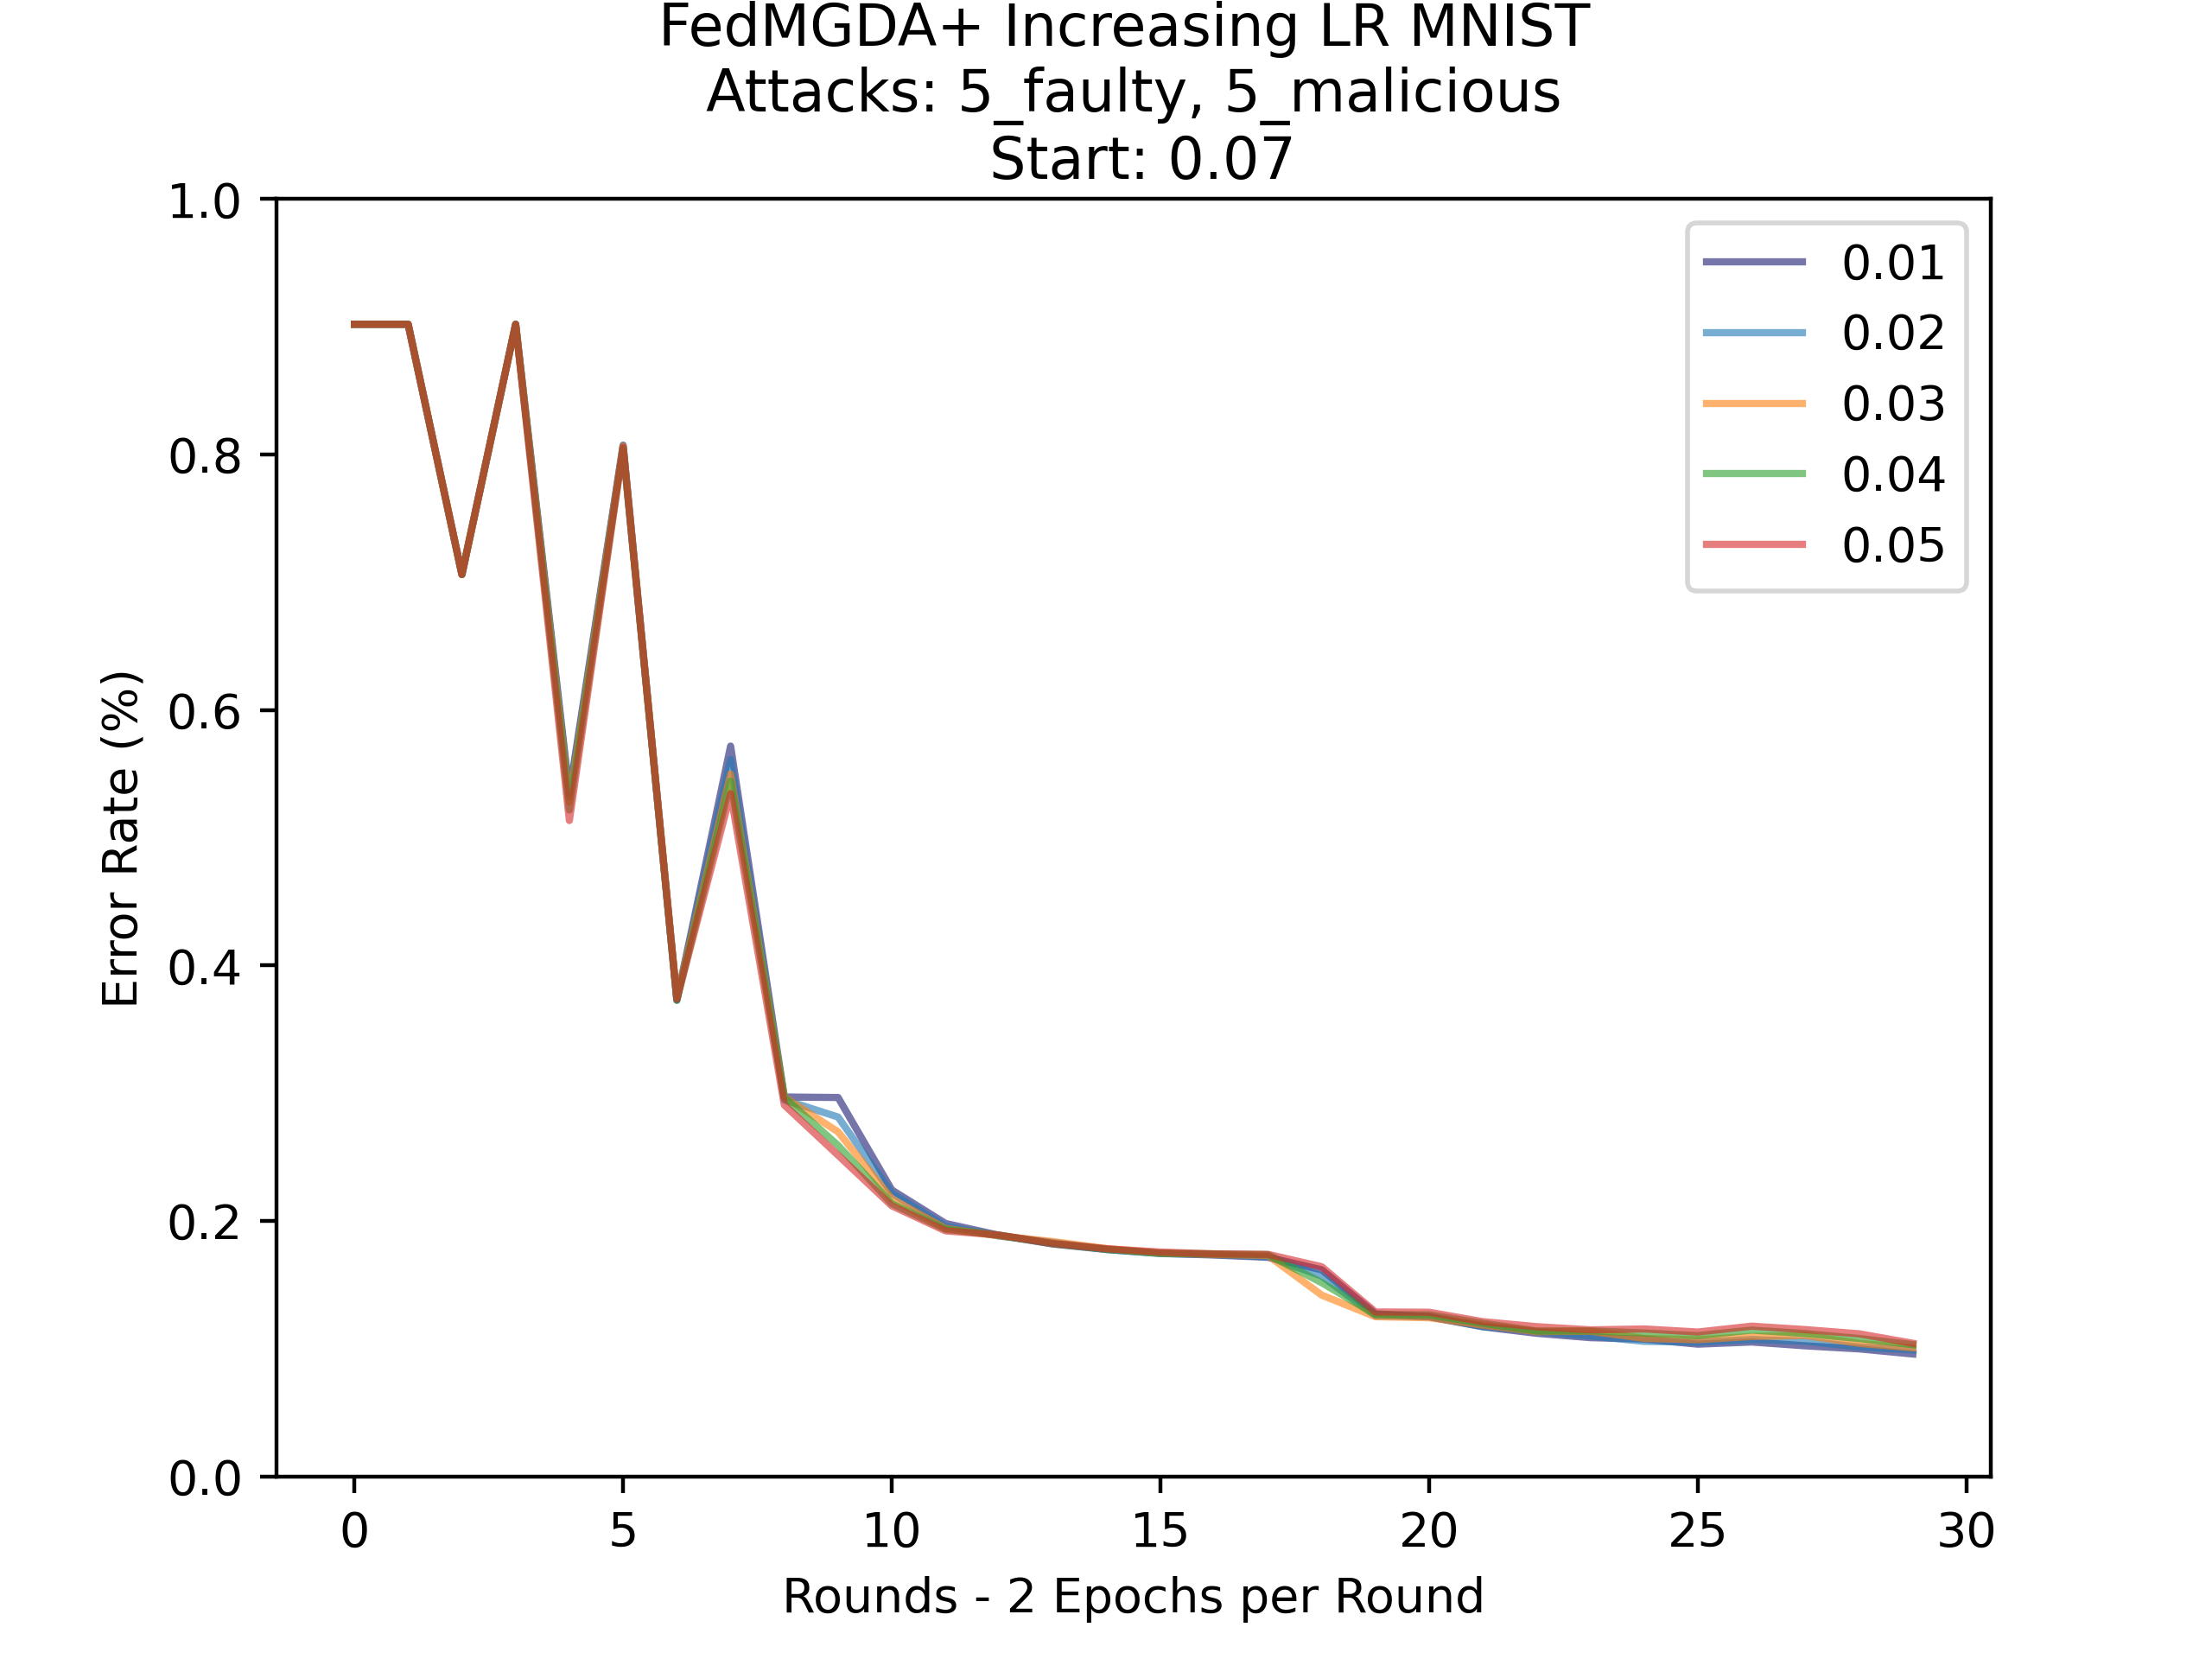
\includegraphics[scale=0.7]{initial/graphs/best_fed_result.png}
    \caption{The Error Rate graph from the best results from FedMGDA+. Notice that the performance doesn't change much but the main importance is the blocking.}
    \label{fig:best_fedmfda+}
\end{figure}

\subsubsection{Through the Looking Glass}
We now generalise our takeaways to our implementation of FedMGDA+. 
Having a more dynamic ability to vary LR will pose a greater threat to byzantine clients.
So, instead of having a fixed start and end, we have a slightly increased starting LR and now have a LR that is based on two things: when clients get blocked and when the error rate increases as opposed to decreasing.
\\ \\
This happens such that when a client gets blocked the LR decreases by a multiplier for each client that is blocked.
This allows a higher starting LR as it can quite quickly decrease once clients start to get blocked.
It also stops benign clients from getting falsely labelled later on.
Also, it is not uncommon that there is some fluctuation of the LR during federated training rounds and so having the LR increase by a set multiplier each time this happens has given some noticeable benefits as well.
It has shown greater promise in the later stages of training where the LR starts to converge but might deviate slightly.
We have seen noticeable corrections that have seemingly reduced the likelihood of late-stage benign clients being flagged as byzantine.
\\ \\
However, the performance of our model was still sub-optimal.
In attacks where only malicious clients were present, sometimes next to no malicious clients were being blocked.
Even on certain combinations of faulty \& malicious attacks, the clients would just start classifying way too many benign clients as byzantine later on.
This caused such poor performance that other weaker aggregators like MKRUM were out-performing it.
\\ \\
We also noticed that it was quite common for the weights of the model to look something akin to [8, 8, 9, 7, 10, \textbf{2}, \textbf{3}, 7, 6, 8, \textbf{1}].
Here the boldened numbers show weights of malicious clients that are very obviously malicious to our eyes but aren't being picked up due to not being negative or getting too low at all.
So, we devise a standard deviation (std)-based approach where if the clients fell below a given threshold that would be two StDs from the mean then it would get blocked.
However, as seems commonplace at this point, an adaptive approach was needed.
When we tried keeping it static, depending on the attack, either clients would not be getting blocked when they needed to be, or too many benign clients would be getting blocked unnecessarily. 
We took a very similar approach to the LR in that when clients got blocked, we increased the multiple of the number of StDs from the mean that it would take before a client got blocked and we decreased the std multiplier whenever the error increased.
\\ \\
This significantly improved the algorithm. While there were still certain attacks that worked better with aggregators like COMED and AFA, Most malicious clients were now getting blocked at a frequency on-par or exceeding that of AFA.
Rather aptly, I dubbed this new method FedMGDA++.

\section{Limitations of Robust Aggregators}
Figuring out where the aggregators thrive and where they fall short is quite crucial to determining their relevant applications or whether or not they should be used in the first place.
So, I went out to see how far the aggregators could be pushed before they either stopped learning or when too many benign clients became blocked.
We used an extreme test case of 15 faulty, 15 malicious or 10 faulty \& 10 malicious clients in the tests, to best demonstrate the aggregator's performance.


\subsection{Malicious Clients}
The first aggregator to fall comes at the five-seven malicious client mark and that is FedAvg.
It mainly starts with a performance degradation [\ref{fig:6mal}] until it simply is no longer able to learn anything of importance.
At this point both AFA and FedMGDA++ are still blocking all of the clients within the first 5 rounds.
All of the other aggregators are not noticing any performance degradation of any sort.
\\ \\
After that not much happens until the 11-12 malicious client point.
Here, AFA is the first to go [\ref{fig:11mal}] with FedMGDA++ and MKRUM not too far behind.
What is most interesting is that AFA is still fully able to recognise all of the malicious clients.
However, it does take up to the 20\textsuperscript{th} federated round before all of them are blocked.
Compare this with FedMGDA++ at 12 and it becomes more clear to see as to why AFA starts to fail earlier.
\\ \\
COMED ends up being the last survivor but slowly has reduced performance (down to around 60\% accuracy) before failing to learn at all.
This happens at the 15 malicious client mark which is pretty much where you would expect to see a median based solution stop being effective.
\\ \\
Something that has place for future research work is how FedMGDA++ is able to still block the majority of malicious clients while not really blocking any benign ones in the process.
This happens until even 15 malicious clients are present and shows its true testament for malicious client detection, even if it has bad performance.
Where future research can really strive is testing out how well a system in which the model is trained once with a robust aggregator with blocking, and then again afterwards without all of the blocked clients.
We believe this to have potential to allow systems that have too many malicious clients to still have the benign clients get a good model at the end of the day.


\subsection{Faulty Clients}
Immediately, FedAvg gets taken out and is not able to handle any faulty clients at all.
Very interestingly though, FedMGDA++ is the next to fall at around seven faulty clients.
What is interesting here is that it takes until about 11 faulty clients before it is completely lost.
It still shows signs and promise of learning at seven [\ref{fig:7faulty}] but just very slowly.
Similarly to with malicious clients, FedMGDA++ is still fully able to block all of the clients all of the way until the end of test at 15 faulty, past when AFA stops being able to.
\\ \\
Speaking of AFA, that is the next to go at 12 faulty clients while COMED is the only survivor even with 15 faulty.
AFA only lasts until about round 14 with the blocking but even then, it is not even blocking all of the faulty clients.
Noticeably, faulty clients are much easier to detect it seems, but they also have far more damaging effects on the model as a whole much earlier on.
\\ \\
Something that was surprising was how when the aggregators stopped being able to work properly, they weren't just forming straight lines as with malicious clients.
Instead, the accuracy was a bit rough and oscillated [\ref{fig:15faulty}], as if there was still some attempt from the model to learn but it just got overwhelmed.


\subsection{Combined Attacks}
Combined, there was nothing extra special about it.
Generally the effects felt were pretty consistent to the previous ones or a combination.
The main interesting part was that at around a combination of six malicious and six faulty, AFA and FedMGDA++ started to stop being able to recognise malicious clients as well.
As the number increased, fewer and fewer got recognised until just the faulty ones got recognised.

\section{Conclusion}
Robust aggregation has a lot of potential and a lot of different methods exist for attempting it.
What caught me off-guard the most was how well COMED did throughout.
It repeatedly was the last one standing and was able to consistently achieve good accuracy.
It really highlighted to importance of a good strategy and what it can accomplish when the applied to the correct problem.
Especially as it is becoming more common to simply slap ML on something and call it a day (\textbf{cough} FedMGDA+), it is important to reason about the problem more logically.
This is something that I aimed to do when I improved upon it and it really showed in the end.
\\ \\
One important thing to note is that while comparing Aggregators, they are not all competing for the same goal.
COMED and MKRUM both don't aim to block malicious clients and as such don't have that more complex overhead of trying to do so correctly.
So, even though it looks as if something like COMED outperforms all others, you could argue that it not blocking any clients means that it isn't on the same level as AFA and FedMGDA++.
Ultimately, it is down to personal preference with how you want to deal with the byzantine clients but it is something to note when deciding on the aggregation strategy.

%%%%%%%%%%%%%%%%%%%%%%%%%%%%%%%%%%%%
\chapter{Free-Riders}
Free-Riders operate by pretending to act as a normal client that is contributing to a model, all while actually contributing nothing.
To successfully achieve this and convince the central server, several clever tactics need to be undertaken to hide as best as possible.
This chapter will be investigating their effectiveness and seeing how well robust aggregators are able to handle them.
The main points of interest will be accuracy and which clients get blocked.
\\ \\
All experiments done have been run on all the previous aggregators. 
In terms of StD and mean tests (as described later), there does not appear to be much difference in distinction.
So FedAvg shall be used for these types of graphs in this section unless otherwise stated.

\section{Main Measure of Defence}
The best way to detect the free-riders from attacks is through the mean and StD of the parameters gradient weights.
Standard clients tend to show a general noisy shape that has an initial increase and then slowly decreases to flat as the model converges [\ref{fig:std_basic}].
\begin{figure}[htbp]
	\centering
    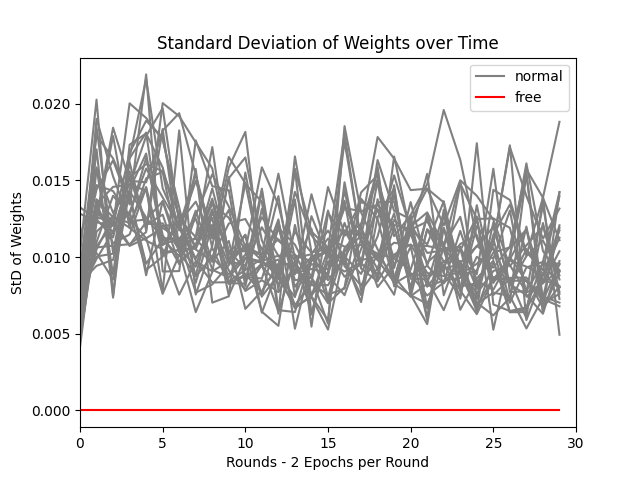
\includegraphics[scale=0.5]{free_riders/graphs/1_free.png}
	\caption{StD Curve for Most Clients Compared to Free-Rider}
	\label{fig:std_basic}
\end{figure}

As you can see, free-riders will have to try and match this general shape in order to stay hidden. 
However, it may be that the central server doesn't find itself in a position where it cares unduly.
Looking at the case where there are 5 free-riders in a basic attack [\ref{fig:5free}], the accuracy tends to be really good all-round with the slight exception of FedMGDA++.
If the main concern of the central server is simply the accuracy at the end of the model, then ultimately it may not be considered an issue.
However, if there is intellectual property or monetary value at stake, free-riders might not be acceptable.


\section{Noise Addition}
For the central server, if all it received was the same model that it sent out, it would be easy to tell which clients are free-riders. 
To counteract this check, the free-riders can simply add some noise to the model so that they can remain more hidden.
This does allow for some more basic blending in but does not quite achieve the same necessary shape. 
However, it is able to demonstrate an ability to give an appearance of remaining hidden [\ref{fig:std_noisy}] through similar visual noise characteristics.
\begin{figure}[htbp]
	\centering
    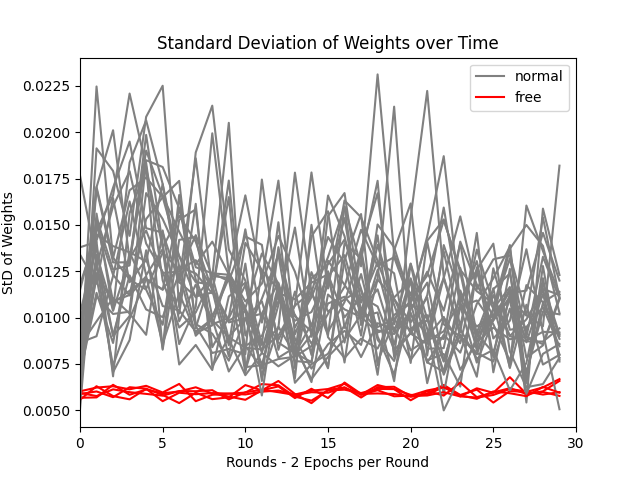
\includegraphics[scale=0.5]{free_riders/graphs/noisy5.png}
	\caption{StD Curve for 5 Noisy Free Riders}
	\label{fig:std_noisy}
\end{figure}

Initially, it might look like there is a blatant distinction between the 2 sets of clients.
However, the noise parameters can be finely tuned such that they can match the amplitude and displacement as is present with the benign clients.
Therefore, the clients can much more seamlessly blend in.
\\ \\
One issue that remains, is that the tuning from the free-riders is somewhat a tricky matter.
From an outside perspective with full control of the system, it can easily be decided what the noise parameters should be.
However, from a free-rider with information only about the global model and itself, it cannot know for sure what the optimal parameters are.
This can be subsidised by investigating the difference in the models and to try and calculate ideal noise patterns from that, but it still lacks accuracy and can ultimately be detected through analysis or through DAGMM energy.

\section{Delta-Weights}
This is where the delta-weight attack comes in.
The idea follows on from the previous section on estimating the noise parameter values whereby you take the delta between the current global model and the previous one.
The difference is then taken and is set to be the free-rider's model gradient weights.

\subsection{Standard Attack}

This has the useful side-effect of having the StD and the mean of the gradient weights to more closely emulate that of a standard client as shown in [\ref{fig:std_delta}].
\begin{figure}[htbp]
	\centering
    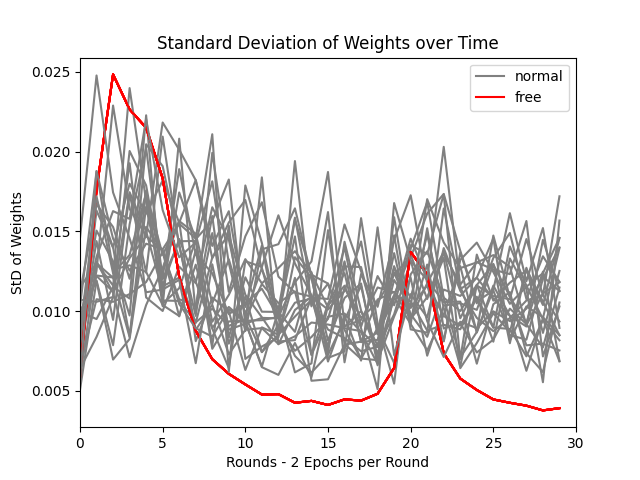
\includegraphics[scale=0.5]{free_riders/graphs/delta8.png}
	\caption{StD Curve for 8 Delta-Attack Free Riders}
	\label{fig:std_delta}
\end{figure}

Now, it's obviously not a perfect solution but it does show the more characteristic increase at the beginning along with the second peak later on that more closely resembles the other clients.
Again, it is not a ultra-finely tuned system but definitely approaches a solution that much more closely resembles a correct one.
\\ \\ 
One basic detection method would be to just check if there are any clients with identical StD characteristics but obviously this attack would benefit from some noise and scaling in places.
This is important to note as ultimately there are an endless amount of possibilities of fine-tuning a free-rider could do to any attack vector and so getting bogged down in the nitty-gritty doesn't contribute much.


\subsection{Privacy Amplification with User Sampling}
When adding privacy amplification, it is important to know if there are points at which the convergence will break down.
This is because it may be that there are just simply too few clients in each aggregation step to do so properly.
Now currently, IID data is being used and so the likelihood of this is not too high, but it is something to at least test and consider.
For the experiments, the value at which the uniform sampling will be cutoff is the p-value and this is what will be altered.
\\ \\
As assumed, the performance degradation is practically none for IID data [\ref{fig:p_test}] with only MKRUM showing some performance loss with very small p-values (0.05 - 0.01).
This only happens for higher number of epochs per round. 
When it is reduced from 10 to 2 (our previously calculated ideal), we see that MKRUM fails much more spectacularly [\ref{fig:p_test_2}] on the lower p-values.
As the clients are sampled uniformly and randomly, it is enough to conclude that the thresholding value does not provide too much of an issue to the performance of the model.
It should be noted that with the addition of malicious/faulty/free-riding clients, the effects of larger amounts of these clients may become exaggerated when the p-value is too low.


\subsection{Privacy Amplified Attack}
With the most advanced attack being based on the difference of two models, it stands to assume that you ideally do not want the clients to have the global model at all to help reduce this attack.
This might not be sensible as the clients could need the global model to converge properly.
So instead, if we were to then reduce the amount of time the clients got hold of the model, then their attack would be less deceptive and become clearer to the outside viewer.
With the help of privacy amplification, we can do just that.
For testing, I used a p-value of 0.3 as a good balance between wanting to maintain accuracy but also wanting to minimise frequency of contribution.
\\ \\
You can see the effects in [\ref{fig:std_priv}] quite clearly and the free-riders are much more noticeable.
\begin{figure}[htbp]
	\centering
    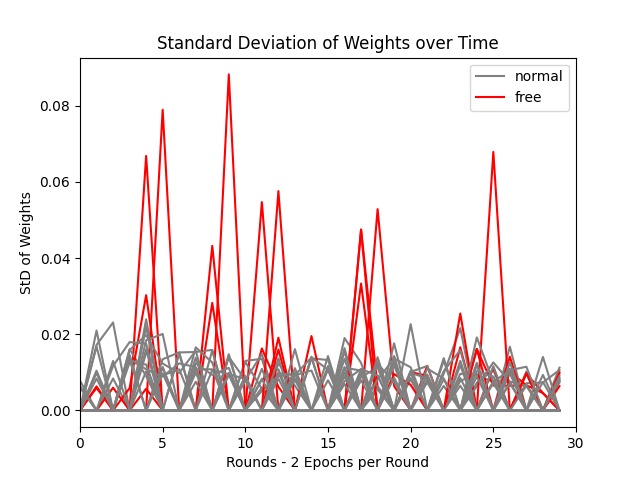
\includegraphics[scale=0.5]{free_riders/graphs/priv5.png}
	\caption{StD Curve for 5 Free-Riders using a Delta-Attack while under Privacy Amplification}
	\label{fig:std_priv}
\end{figure}

The graph shows a lot of data at zero as well and that's just because the gradient weights will be non-existent if they haven't been trained.


\section{Robust Aggregation}
The method by which typical robust aggregators go about aggregating is through identifying and not including outliers (or weighting them low) in the process.
However, by their very nature, free-riders are not outliers in the sense that their parameters are very benign if anything.
They are the essentially the most medium clients from the previous round. 
It is unlikely they would be detected at all by the robust aggregators.

\subsection{Performance}
There was also the matter of performance as having degraded model performance with aggregators trying to do fancy things is really not ideal.
On the low end, performance was not an issue an across the board [\ref{fig:no_dmg}] and only with the addition of privacy amplification did MKRUM suffer [\ref{fig:mkrum_suf}] even with very few free-riding clients.
\\ \\
In general, the performance of the models slowly decreased as more free-riders were added.
FedMGDA++ and MKRUM were more badly affected but it was very much a gentle decrease.
The more interesting point to note was the transition over the halfway point [\ref{fig:comed_broken}] where it went from 14 to 16 malicious free-riders.
This is noteworthy due to it again highlighting COMED's weakness around this point as an aggregator and how it so quickly falls down.
Especially as the other aggregators then proceed to essentially not change much more than normal and are capable of aggregating at a rate such that the decline in accuracy is fairly constant.
\\ \\
The reason the other aggregators don't fall short as badly, is because the free-riders act more as an LR softener.
Essentially, they slow down the rate at which the model converges as you are just adding a bunch of dampening parameters, that are the previous model, to the next global model.
This is why you mainly just see the curves for things like FedAvg, AFA and MKRUM just be at a shallower angle as opposed to having the final position be too much higher.
\begin{figure}[htbp]
	\centering
    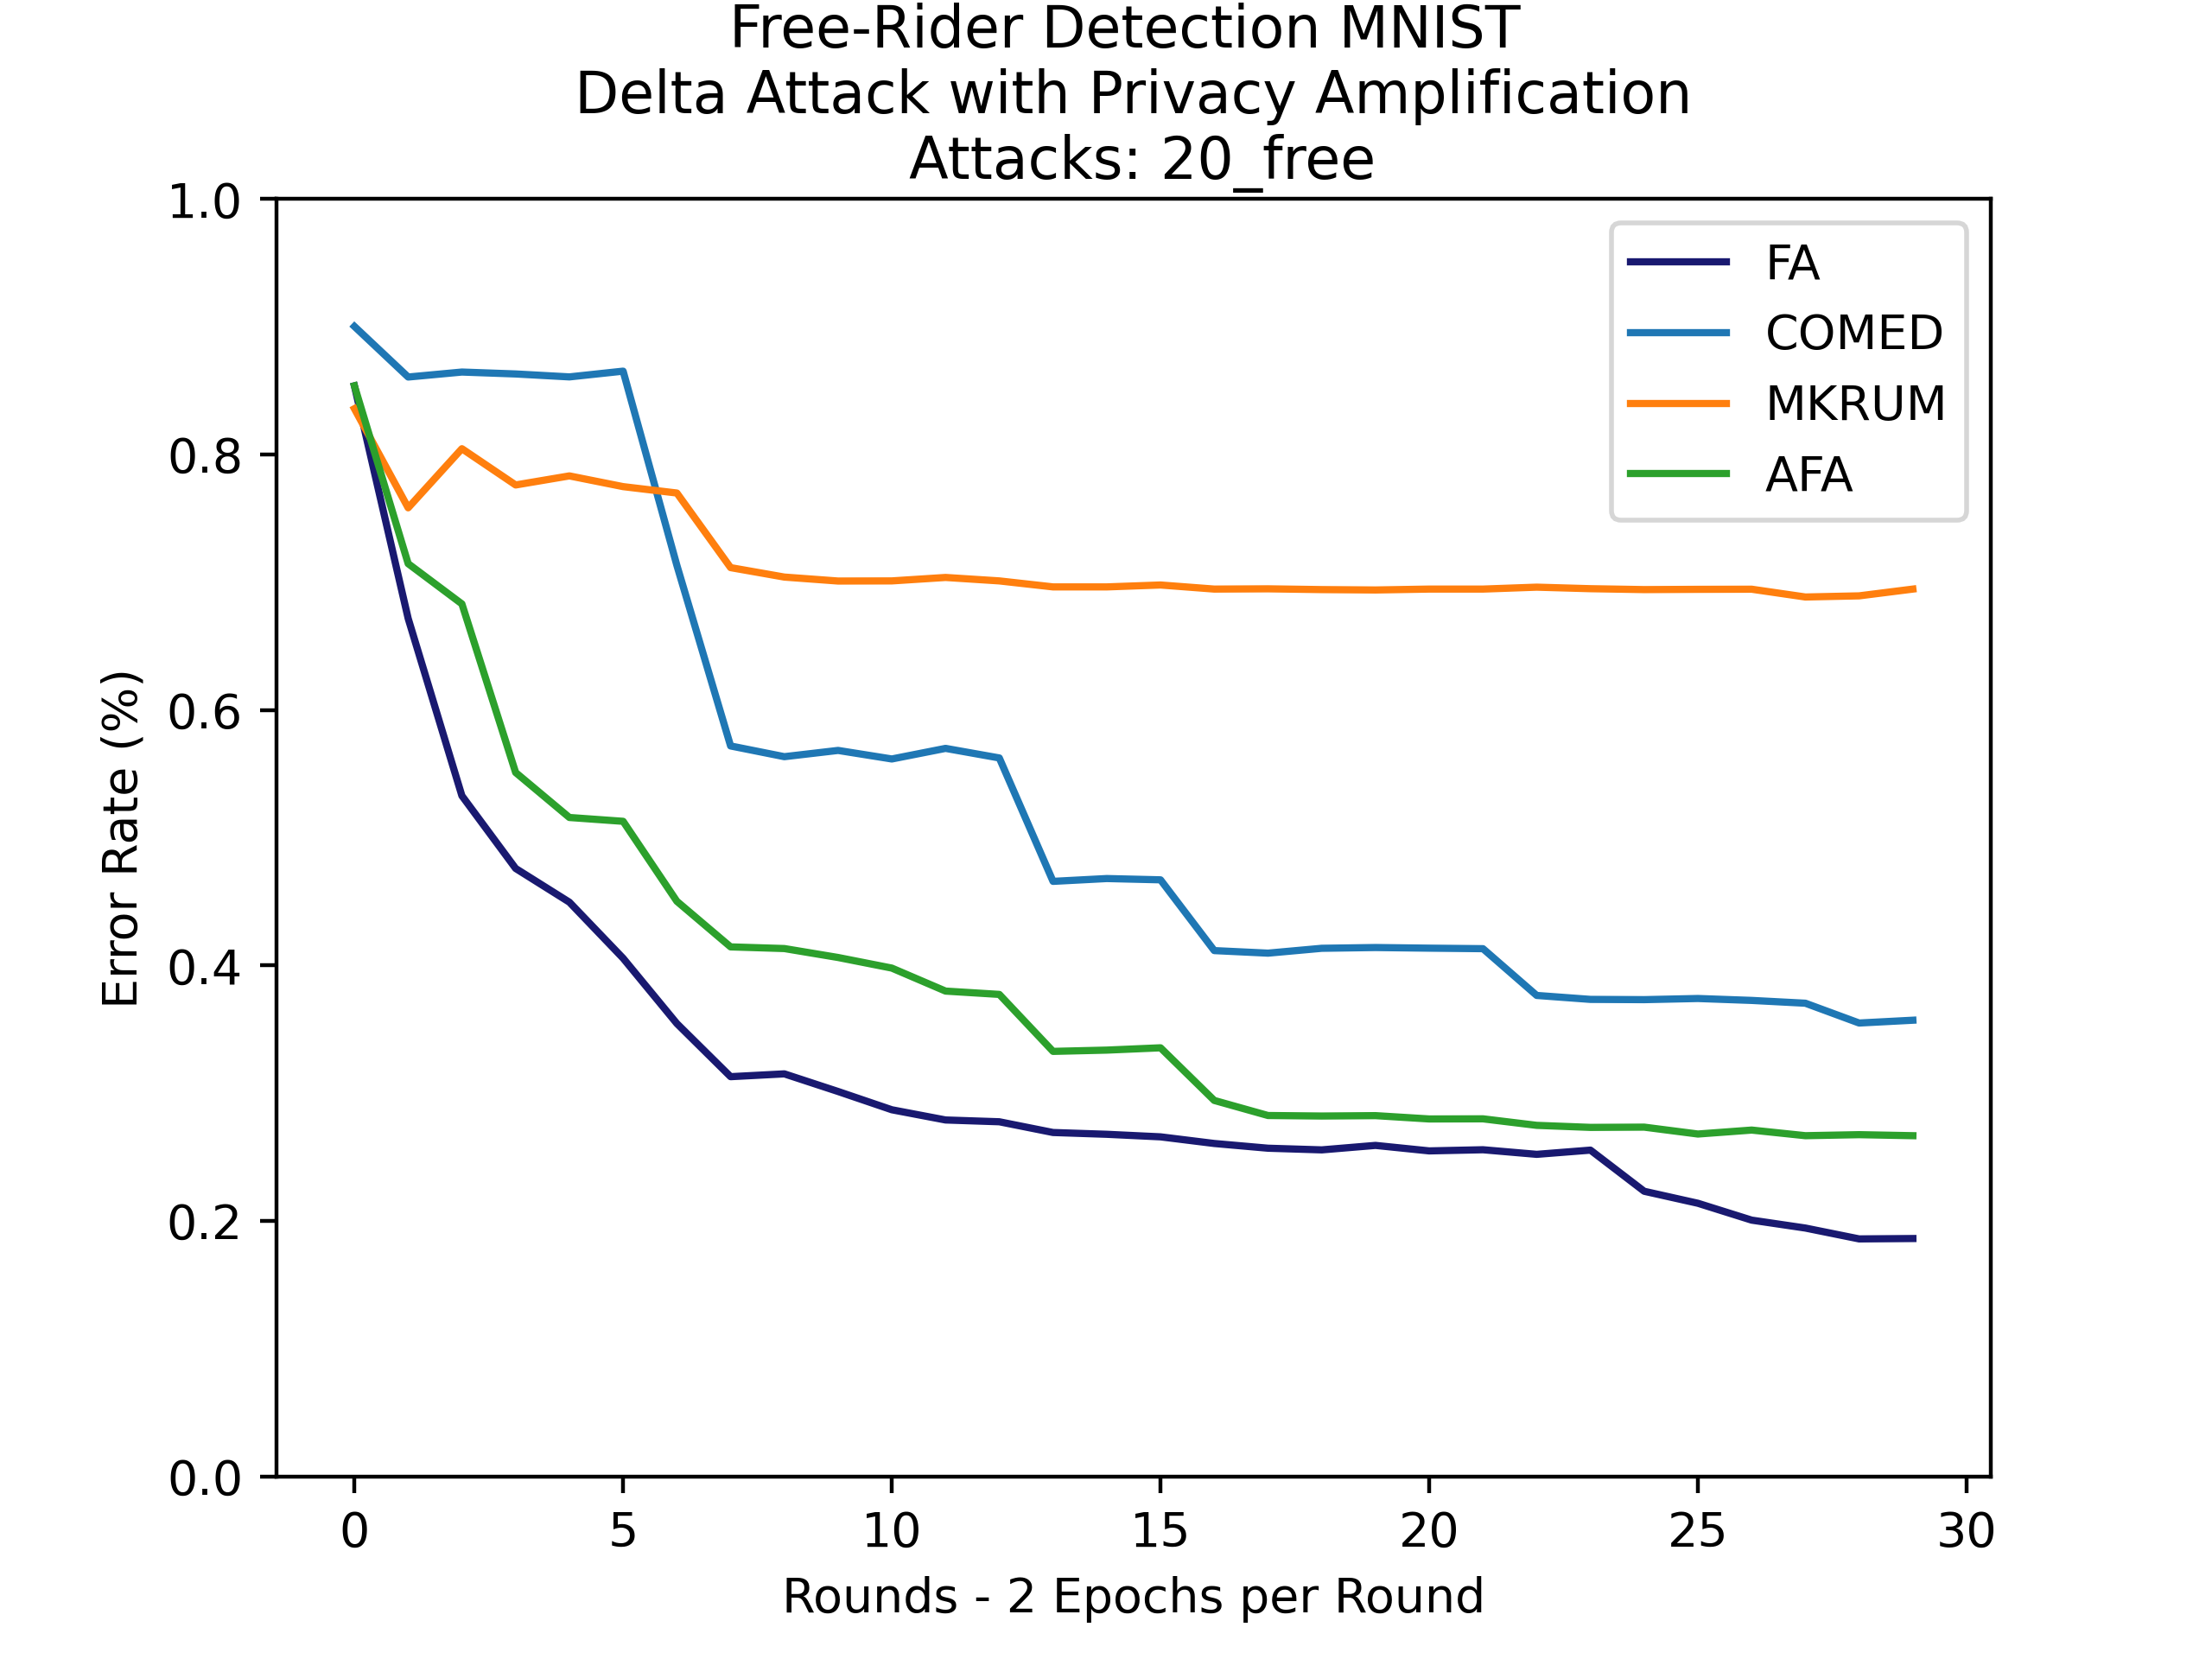
\includegraphics[scale=0.5]{free_riders/graphs/priv20.png}
	\caption{Error Rate of 20 Free-Riders with Delta-Weight Attacks under Privacy Amplification}
	\label{fig:priv20}
\end{figure}

The one exception to this is then the privacy amplification defence, where all of the aggregators are seen to be struggling much more in comparison [\ref{fig:priv20}].
What's fascinating is seeing the sudden drops that occur with COMED, which shows that when the sampling has chosen a set of clients that contains more than 50\% benign.
This leads to a conclusion that might seem odd at first.
If you were to be prioritising the accuracy of the model, then you'd actually not want to employ the privacy amplification defence as it does more damage than just letting the free-riders be.

\subsection{Blocking Issues}
One thing that stood out to me initially was the very poor performance from FedMGDA++ and how it noticeably became to worst affected as the number of free-riders increased.
It ended up being quite a simple issue, the aggregator was pretty much just identifying the benign clients to be the outliers!
This was happening as early on as with only 2 free-riders and 10 benign clients were getting blocked!
\\ \\
The main factor which caused the decrease in the accuracy was simply that with more free-riders, FedMGDA++ thought itself to be getting more certain as to which clients were malicious when in fact it was doing the complete opposite.
This caused the benign clients to be getting blocked earlier and earlier and that's what causes the flat-lining that you see in experiments such as [\ref{fig:flat_line}].
This carries onto about the 15\textsuperscript{th} round, where from then on out, all of the benign clients are getting blocked and so no learning can take place.
This happens to AFA too at higher free-rider counts but to a much lesser extent and AFA never blocks more than 5 benign clients, lending it to still be able to learn at a decent-ish rate.

\begin{figure}[htbp]
	\centering
    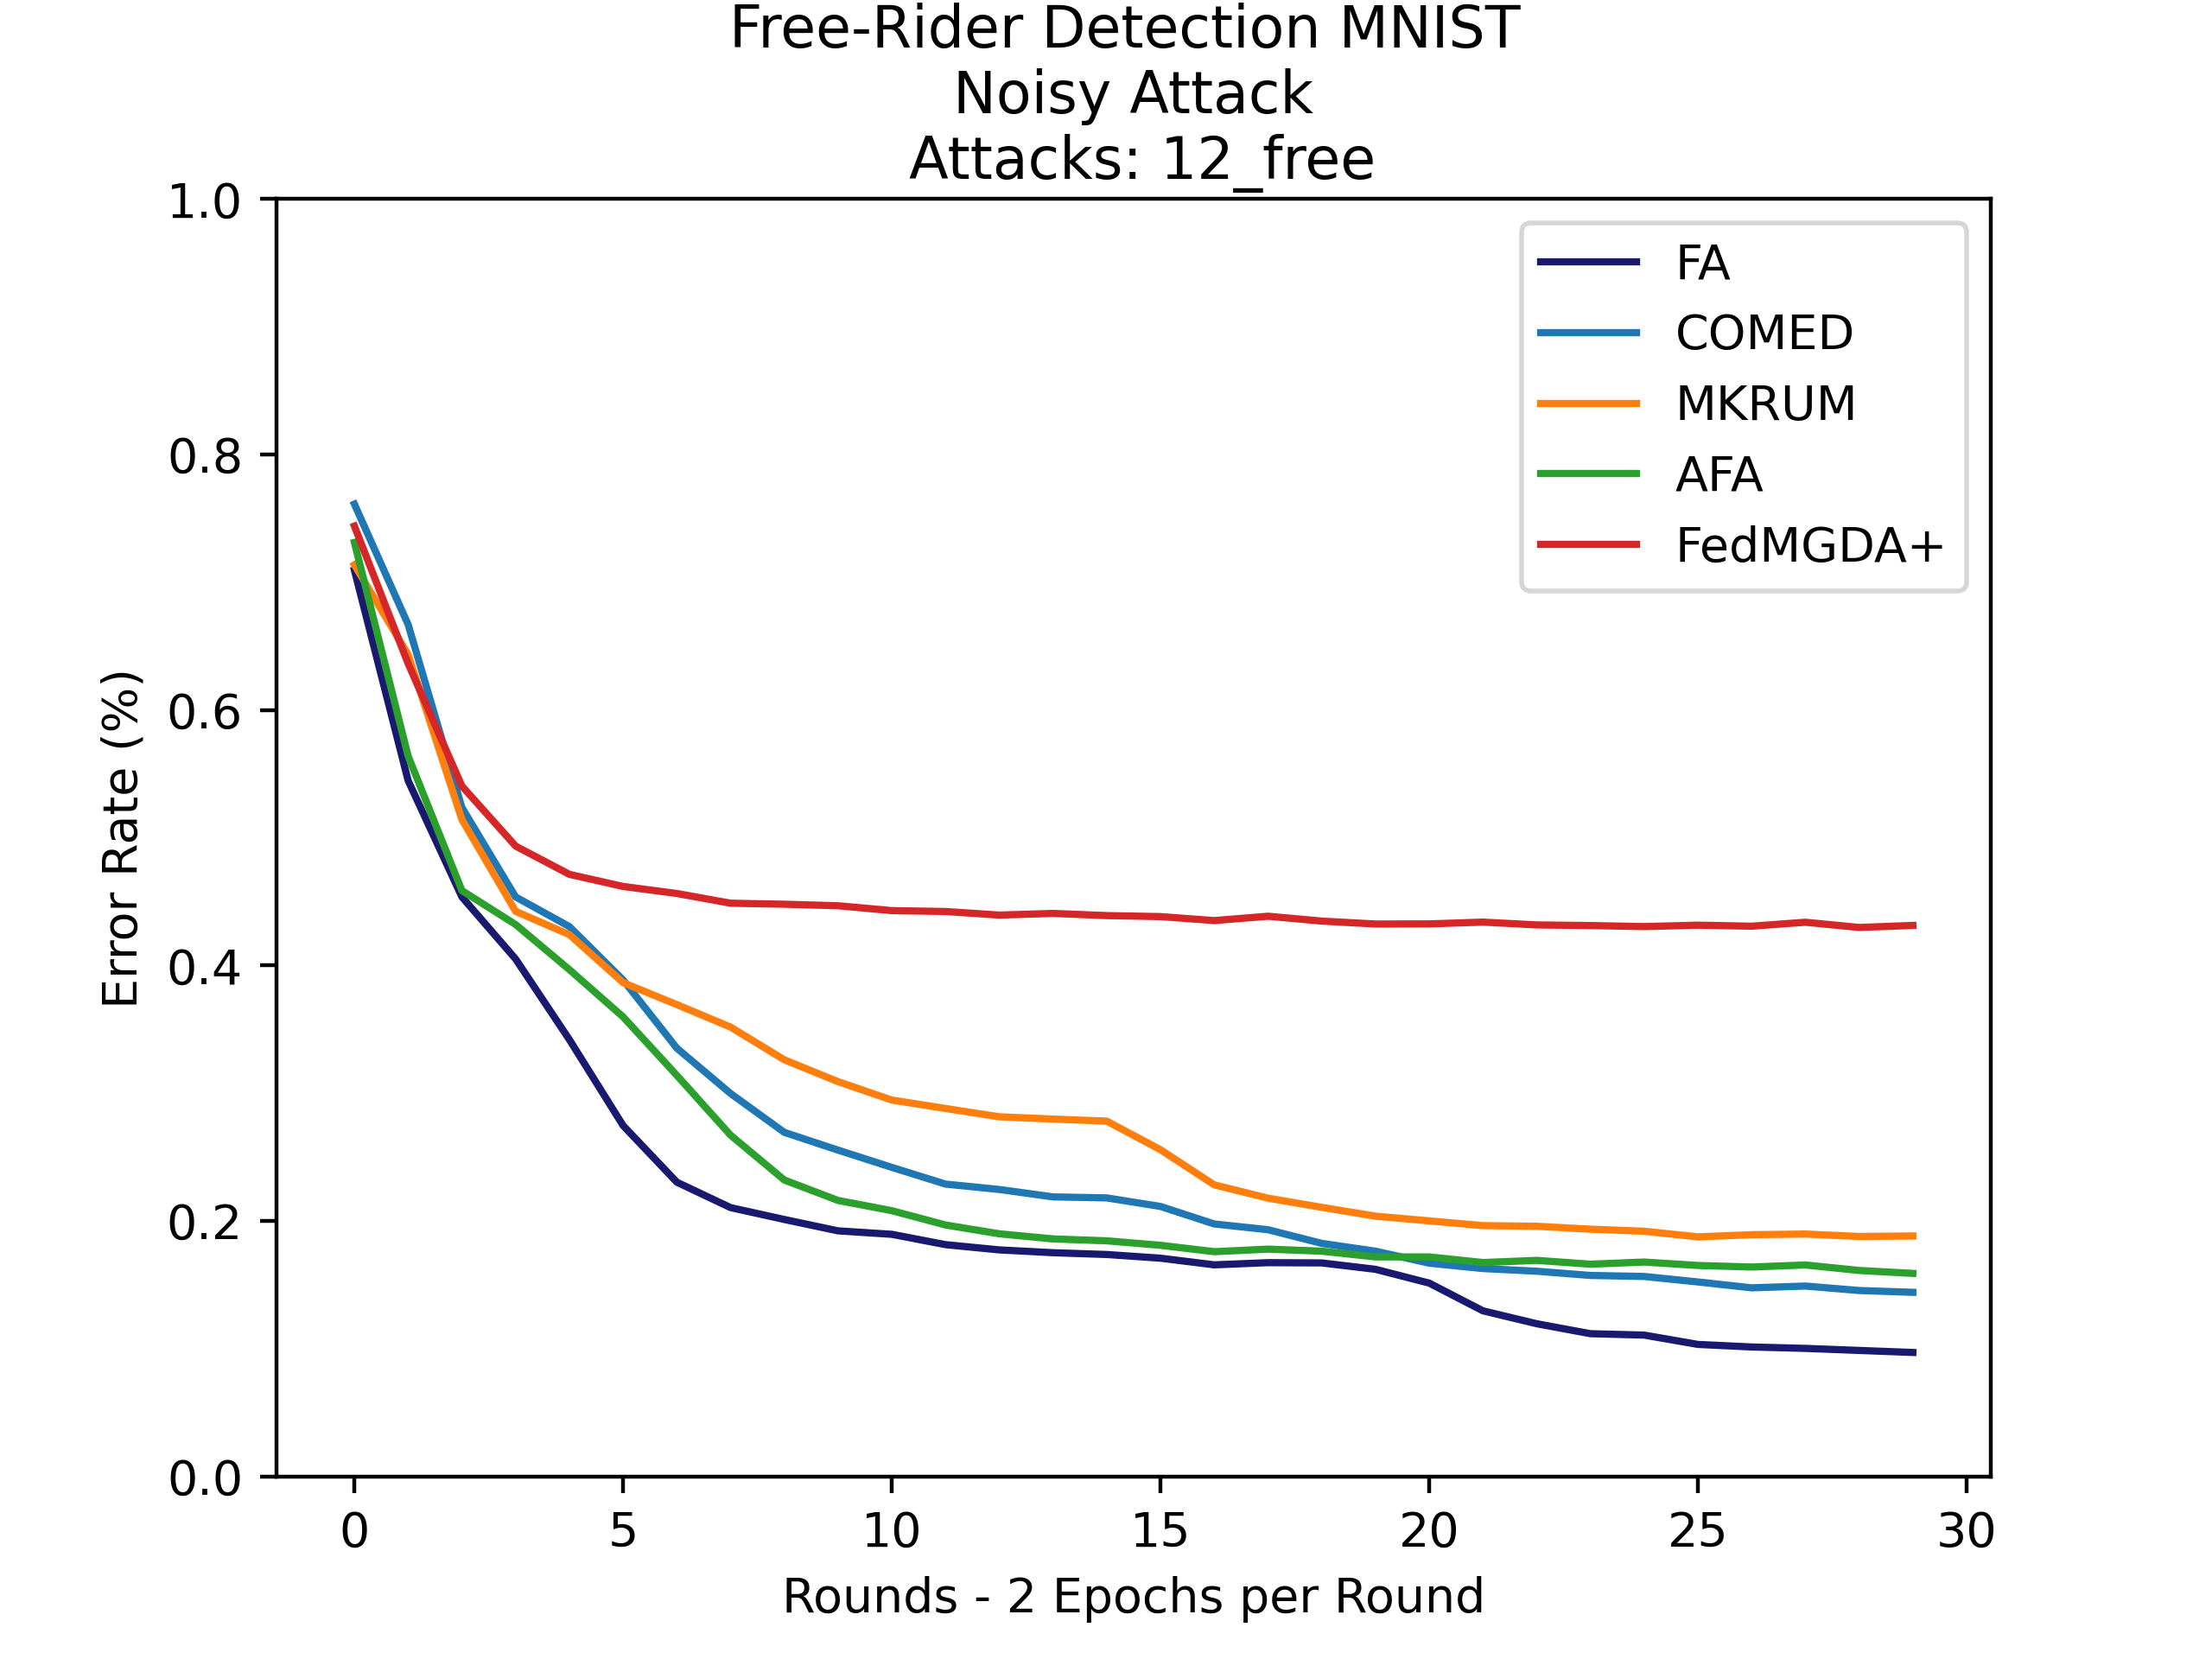
\includegraphics[scale=0.5]{free_riders/graphs/flat_line.png}
	\caption{Error Rate Graph Showing the Flat-Lining of FedMGDA++ once all of the Benign Clients are Blocked}
	\label{fig:flat_line}
\end{figure}


\section{Conclusion}
Overall, free-riders provide an interesting problem in the field of federated learning.
On the one hand, they do very minimal damage and cannot be simply detected and blocked using traditional robust aggregation methods.
On the other hand, they can be capable of masking themselves with fake informational noise to great extents and are ultimately providing fake information to the global model.
\\ \\
It poses a peculiar threat and yet through evaluation of the performance, seems to show no characteristics of being one.
Now, robust aggregators weren't built for this purpose and that is precisely why other methods for detection have been covered.
Ultimately, the global model would benefit more without them and the clients behind the free-riders are getting this model for free and so it really comes down to whether or not either of these things matter much to the specific situation.


%%%%%%%%%%%%%%%%%%%%%%%%%%%%%%%%%%%%
\chapter[FedPADRC]{Personalised \& Adaptive Dimension Reducing Clustering Aggregation}
\label{chap:fedpadrc}
Throughout all of the various aggregation methods covered with and without experimentation, trying to find good ideas and sensible applications of them has been an end goal.
Ultimately, none of the robust aggregators have performed as well as I would have liked on the higher numbers of malicious clients and tend to have reduced accuracy if anything.
This lead me down the path of trying to use ideas from current aggregators and methods in federated learning to try to improve on the SotA.
\\ \\
My goals for creating a better robust aggregator are:
\begin{itemize}
    \item Better understand the robust aggregator space in federated learning.
    \item Enhance current aggregation methods through clustering.
    \item Handle more malicious clients than any other robust aggregator.
    \item Be able to handle free-riders better than other aggregators.
\end{itemize}
Throughout all that I wish to include in the aggregator, I name it FedPADRC (Personalised and Adaptive Dimension Reducing Clustering).


\section{Clustering}
Initially, I thought about clustering similar models together through K-Means Clustering.
Similar ideas like this have been tried already \cite{cluster_robagg} but didn't really attempt anything that I would personally call robust (even if they claimed otherwise).
So, I wanted to build upon this idea by instead using some combination of FedAvg, COMED and MKRUM to do the aggregation.
I couldn't really use AFA of FedMGDA++ as they both relied on learned information about the whole system.
FedMGDA++ especially relied on having all the clients present at every step on never subsets of the clients.
\\ \\ 
However, robustly aggregating at only the clustering stage seemed like it would very easily be abused by a coordinated attack of malicious clients.
This is because malicious clients would end up having similar models due to their coordinated attack strategy being the same.
Therefore, there would always be at least one cluster of just malicious clients.
Something like COMED might be able to handle this better but it was something definitely worth investigating.
So, I would then also need to have robust aggregation happen when aggregating the cluster centres together to form the end model (something that hadn't been done before).
\\ \\
Prior to any testing, one thing that is important to bring up is that K-Means Clustering is a very computationally intensive algorithm to run.
Increasing the number of clients beyond the 30 here to systems with orders of magnitudes of more clients might not be a sustainable process.

\subsection{Aggregator Capabilities}
There are 9 different combinations of aggregators that I can try but realistically having FedAvg be the aggregator in the second aggregation step is pretty futile as malicious clients are pretty guaranteed to get through and damage the model.
Also, for trying to segregate the clients' models from each other, more training than the standard two epochs will need to be done.
So, I increased the number of epochs per round to 10 when we're clustering so that each client's model can appropriately represent itself before it is clustered.
\\ \\
Very early on it appeared to be apparent that using MKRUM as an external and internal aggregator proved pretty much useless.
This was because with just one attack, it's performance was all over the place [\ref{fig:mkrum_bad}] with any internal aggregator.
However, COMED on the other hand seemed to steam-roll right through any number of malicious clients, only starting to fail at around 22 malicious clients.
This is incredible as this outperforms any of the other robust aggregation methods tested!
\begin{figure}[htbp]
	\centering
    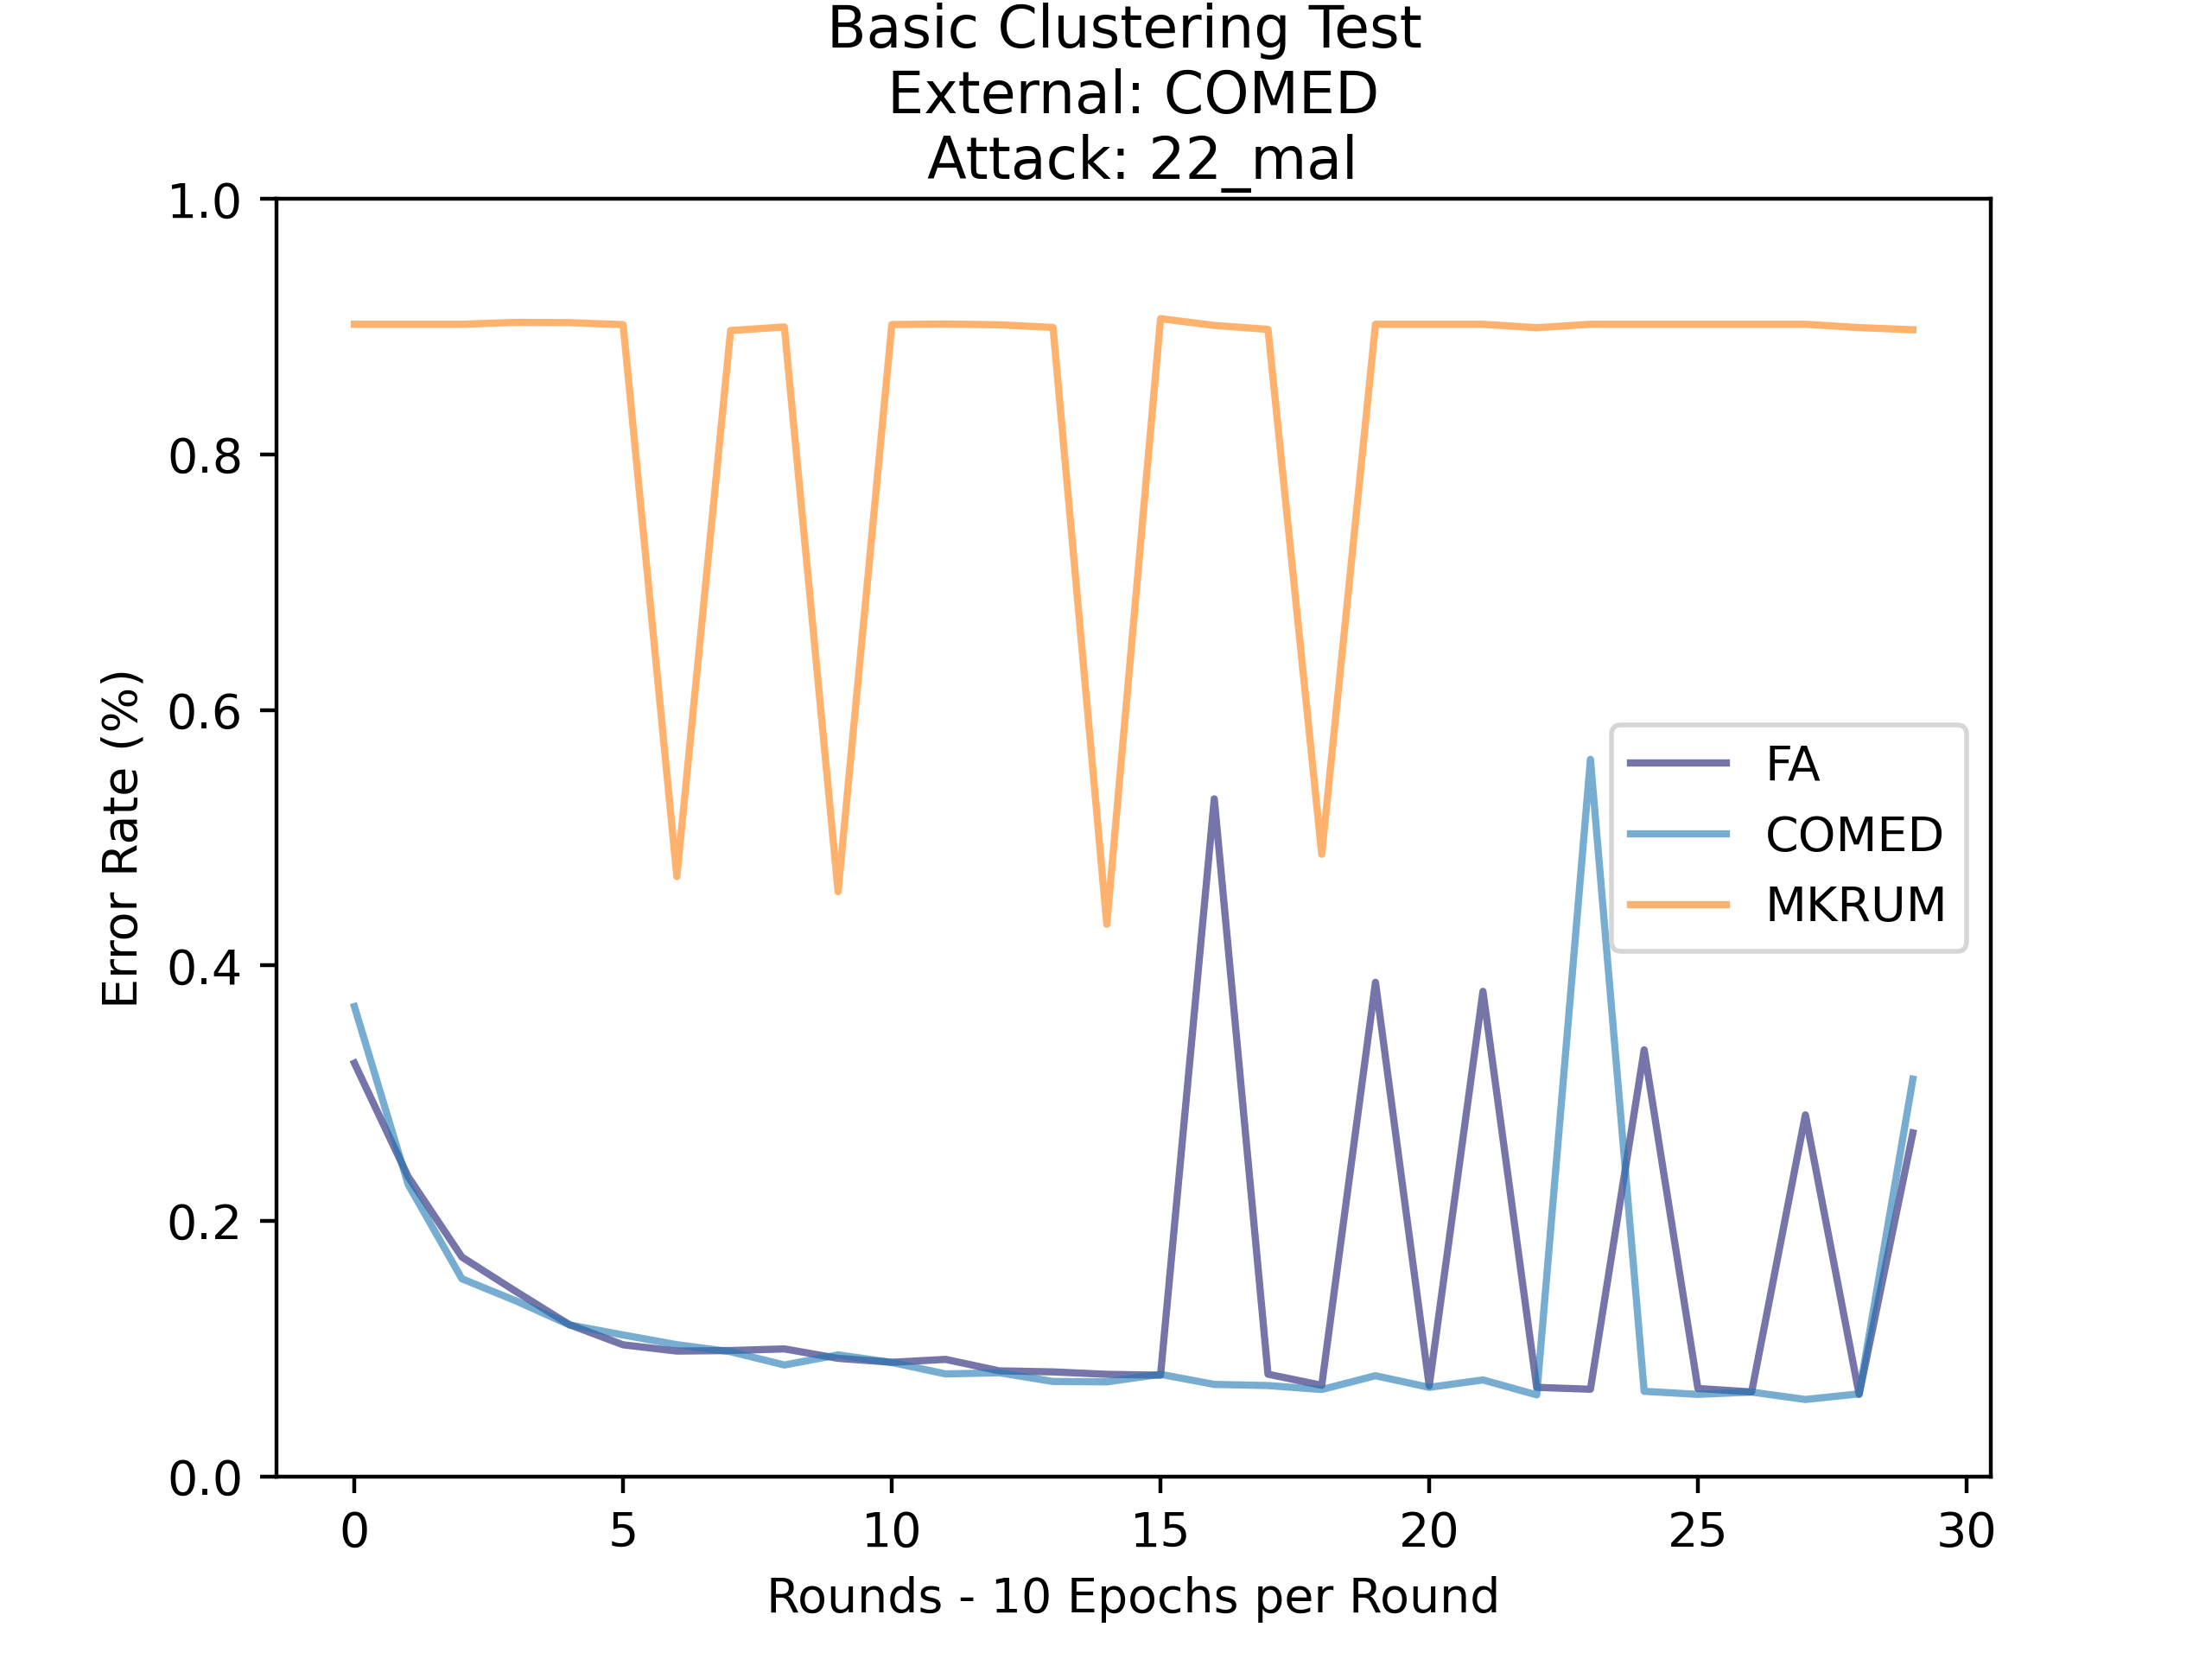
\includegraphics[scale=0.5]{my_agg/graphs/cluster_comed_22.png}
	\caption{Error Rate of K-Means Clustering with COMED as the External Aggregator - 22 Malicious Clients}
	\label{fig:comed_22}
\end{figure}
Throughout testing, both FedAvg and COMED performed similarly in their internal ability to aggregate, with it only varying later on.
One thing to note is that when the data is non-IID, it might not be as simple as that and FedAvg might start to outperform COMED through its increased data use.
\\ \\
What's also interesting to see is the extremely quick convergence of the model.
This is most likely due to no interference from the malicious clients in the first half of the total number of rounds.
You can also clearly see that the model itself is over-fitting and should realistically only be lasting for 10-15 rounds or so.
This would then help with the later stage spikes that we see.
\\ \\
It didn't quite end there though, as for some very strange reason, MKRUM's performance appeared to get better with more malicious clients being added.
This was such that I was seeing performance from MKRUM being used as an external aggregator compared to COMED at more than 22 malicious clients.
Now, this doesn't then lead me to believe that overall MKRUM performs better, just that it has its very unique and weird moments of performance.
Overall, I believe that using FedAvg to aggregate the clients within the clusters and using COMED to aggregate the cluster centres is the best way forward.


\subsection{Finding the Optimal K}
When it comes to K-Means Clustering, finding the best K-value to use is extremely important to ensure that the data is properly split up and segmented.
Luckily, it is not a particularly complex task and normally just requires testing out the different K-values and using something called the "Elbow Method" to determine which is the best.
\\ \\
The elbow method is when you plot the the number of clusters against some distance/scoring metric.
This could be their literal distance, sum of squared distances, based on accuracy etc.
In plotting there will be a more highlighted point [\ref{fig:elbow}] where the rate of change drastically decreases.
This indicates that further increases in the K-value result in not much benefit and would most likely be over-fitting the data.
\begin{figure}[htbp]
	\centering
    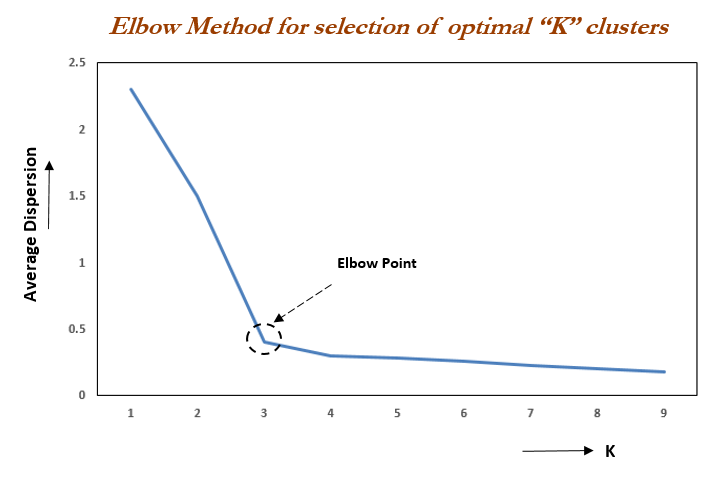
\includegraphics[scale=0.5]{my_agg/graphs/elbow.png}
	\caption{Elbow Method with Highlighted Optimal K-value \cite{oreily_elbow}}
	\label{fig:elbow}
\end{figure}
\\ \\
For the scoring metric I decided to plot the sum of the distances that each model is away from its designated cluster and total it for each value of K from 1 to 30.
Now, there are definitely less hard-coded solutions than this and ultimately using a solution that would have this K-value change would be the most ideal.
However, to recalculate this at every federated round takes minutes for even small models like with MNIST.
So, realistically trying to get a rough idea of the values of K that would be more desirable is the more sensible choice.
\\ \\
Funnily enough, there ended up not being any particular point that could be realistically identified as the elbow point.
I did the above calculations for no attacks, 5 and 20 malicious at rounds 0, 5 and 20 [\ref{fig:k_elbow}].
This was so that I was able to see how representation of the data changed throughout so I wasn't simply basing my analysis from 1 point.
\\ \\
\begin{figure}[htbp]
	\centering
    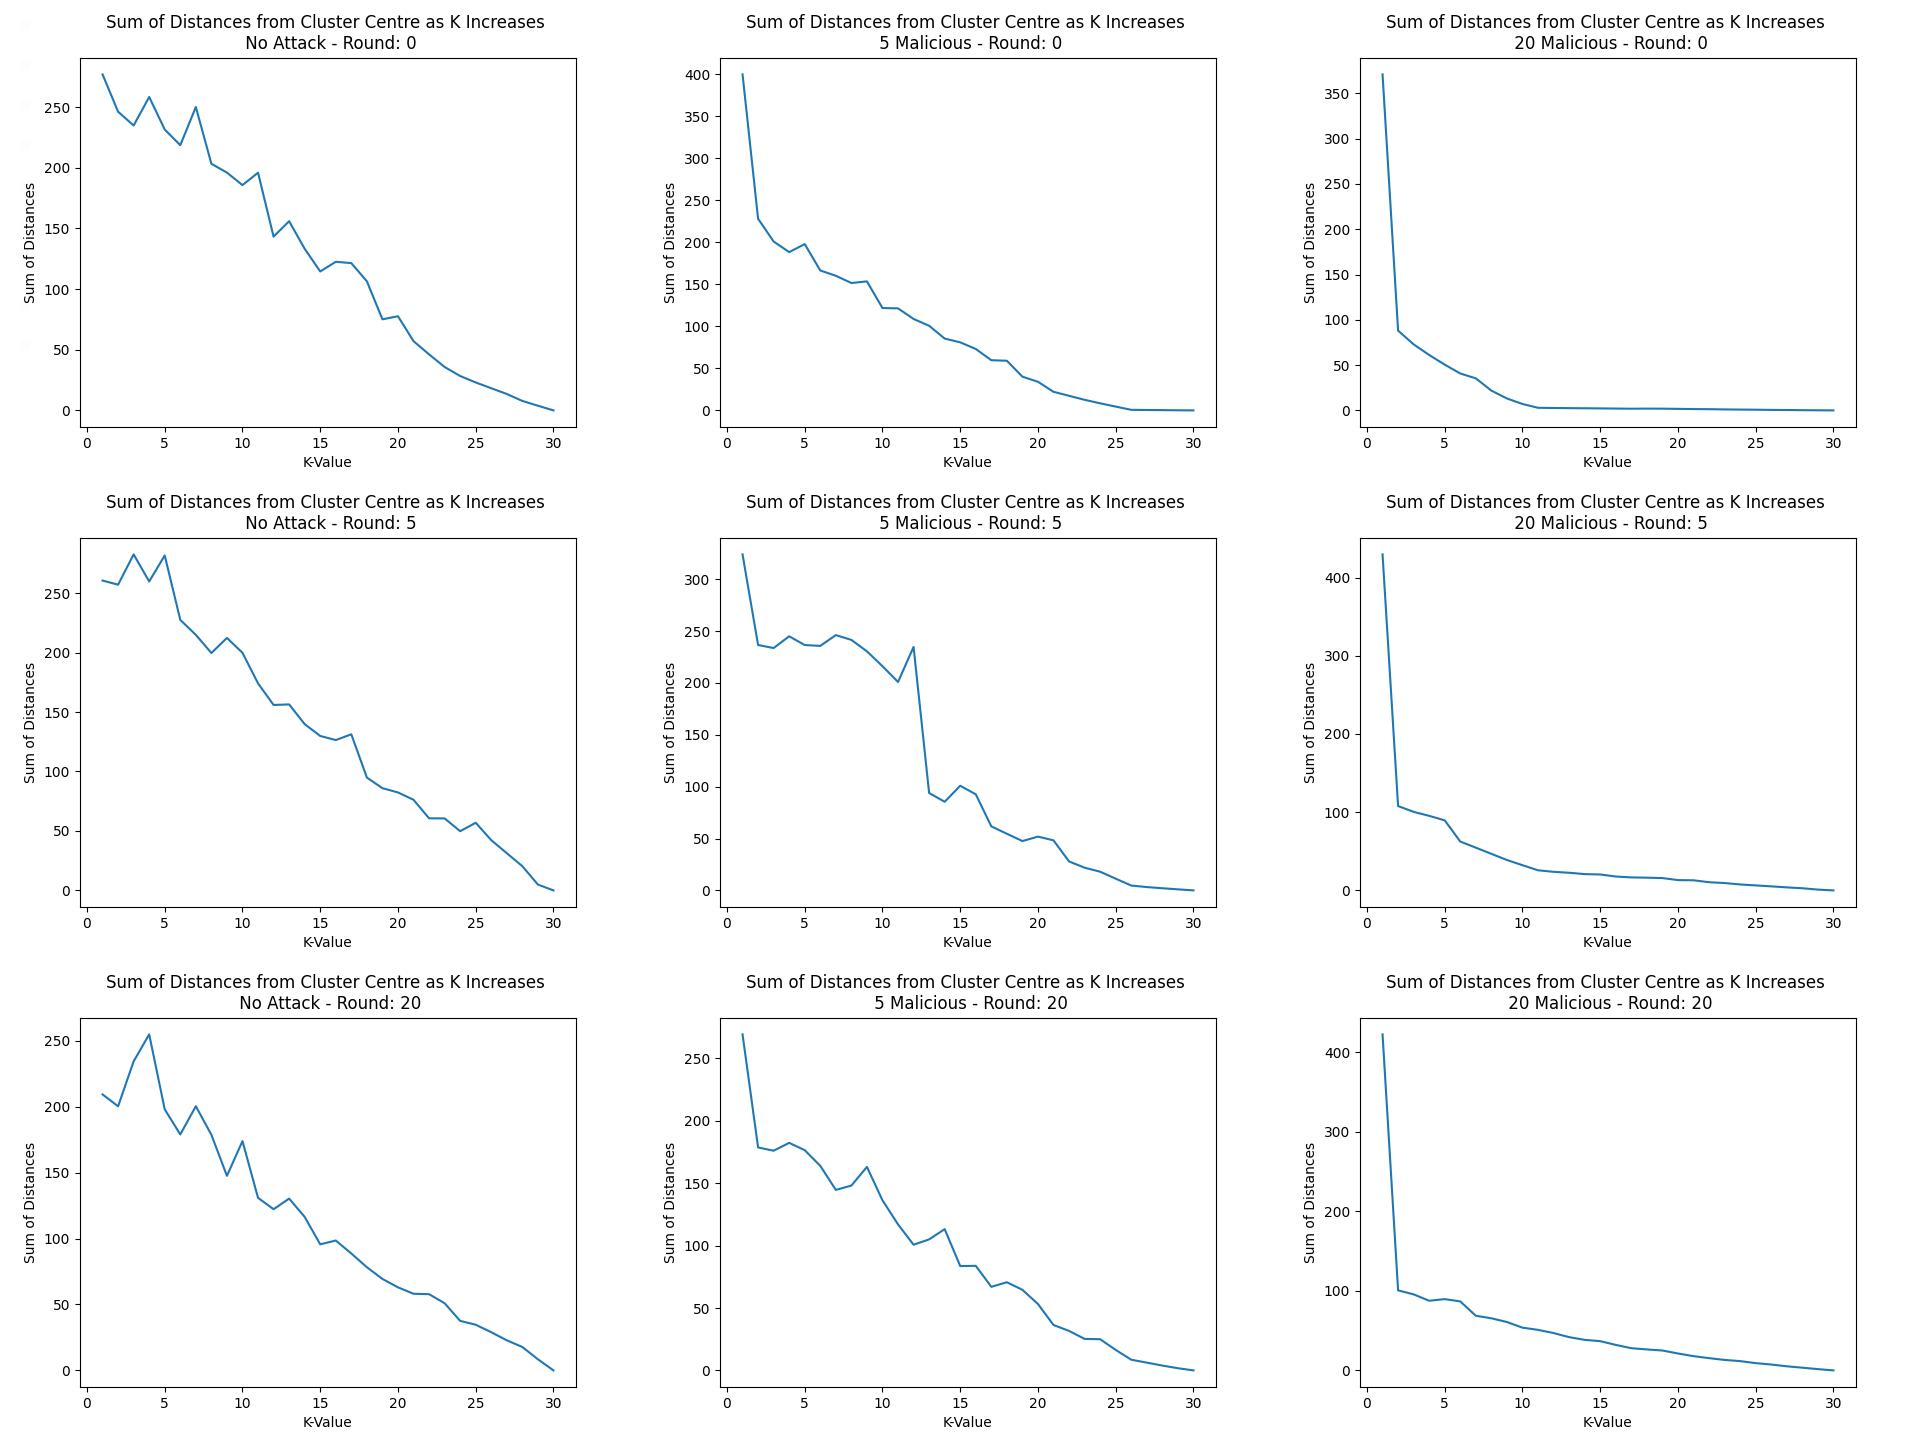
\includegraphics[scale=0.25]{my_agg/graphs/k_elbow.png}
	\caption{Finding the Elbow Point for K-Means Clustering}
	\label{fig:k_elbow}
\end{figure}
\\ \\
Under no attacks, the line was a constant gradient on average and gave no hint of an optimum point.
Under five malicious there were similar characteristics but with a slightly steeper descent at first, potentially hinting at some K-value around four.
At 20 malicious is where things get weird and it is almost like a K of two is the best.
\\ \\
Interpreting these results is interesting to say the least, but one last method I can try is to see what the final and/or minimum error rate values are at each K and see if that can shed any more light on the situation.
What I am expecting is that there won't be much difference with 0 attacks but having a good K value will be more and more important with 5 and 20 as that is where you'll see damage starting to be being done.
\begin{center}
    \begin{longtable}{ |c|c|c|c|c|c|c|c|c|c|c|c|c| }
    \caption{Error Rate (\%) as K Changes}
    \label{tbl:k_error_rate}
    \hline
    K & 1 & 2 & 3 & 4 & 5 & 6 & 7 & 8 & ... & 15 & ... & 30 \\ \hline
    \multicolumn{13}{|c|}{} \\ \hline
    0-Min & 5.3 & 7.4 & \textbf{5.7}	& \textbf{5.7}	& \textbf{5.4}	& 5.3	& 5.3	& 5.1 & ...	& 5.4 & ... & 5.4 \\ \hline
    0-Final & 5.3	& 7.9	& \textbf{5.8}	& \textbf{5.8}	& \textbf{5.4}	& 5.5	& 5.6	& 5.1 & ...	& 5.4 & ...  & 5.4 \\ \hline
    \multicolumn{13}{|c|}{} \\ \hline
    5-Min & 8.8 &	90.2 &	14.1 &	\textbf{9.4} &	\textbf{7.2} &	\textbf{6.5} &	6.3 &	6.0 & ... &	5.6 & ...  & 7.3 \\ \hline
    5-Final & 28.6	& 90.2	& 16.2	& \textbf{9.4}	& \textbf{7.9}	& \textbf{6.5}	& 6.3	& 6.0 & ...	& 5.8 & ...  & 7.5 \\ \hline
    \multicolumn{13}{|c|}{} \\ \hline
    20-Min & 90.2	& 90.2	& 13.4	& \textbf{9.4}	& \textbf{7.3}	& \textbf{7.4}	& 6.5	& 6.4 & ...	& 25.4 & ...  & 89.7 \\ \hline
    20-Final & 90.2	& 90.2	& 16.39	& \textbf{9.82}	& \textbf{8.24}	& \textbf{7.4}	& 6.72	& 11.9	& ...	& 26.94 & ...  & 90.2 \\ \hline
    \end{longtable}
\end{center}
Through setting the number of rounds to 15 to stop over-fitting and remove the peaks near the end, we can now see how the solutions perform at various points in Table \ref{tbl:k_error_rate}.
Seeing the no attack error rates really seemed to fit perfectly with the previous test done as the value doesn't change too much [\ref{fig:k_elbow_0}] except when K is two.
After about the halfway point, K seems to do a little worse as well on average, indicating that it's probably become too high (although it's very minimal).
\\ \\
Where things start to change a bit is when we increase the number of malicious clients to five.
Here, we now notice [\ref{fig:k_elbow_5}] that K has to be a minimum of three for the clustering to work properly.
Going any higher than six/seven gives no improvement and would be overkill in this situation.
It should be noted that right at the very end, when the algorithm is essentially just COMED by itself, there is a gentle increase in the error rate.

\begin{figure}[htbp]
	\centering
    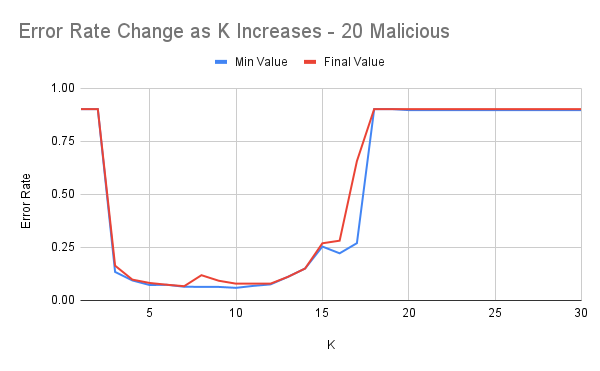
\includegraphics[scale=0.55]{my_agg/graphs/k_elbow_20.png}
	\caption{Error Rate As K Increases - 20 Malicious}
	\label{fig:k_elbow_20}
\end{figure}

Finally, we hit some good data with 20 malicious clients [\ref{fig:k_elbow_20}] as there is a proper U-shape to the error rate.
This further highlights that between three and five is the optimum number for K with the elbow-point being at about three or four.
Noticing that the final value at K=3 is slightly higher than the minimum value suggests that the solution there is getting a bit worse nearer to the end of the federated rounds.
This leads me to conclude that a K of around five is the optimal for this instance but in general terms, values between three and seven should probably work fine.



\section{Dimension Reduction}
When it comes to clustering the data, performing it on the entire model's parameters is very much a noisy affair as there will be plenty of parameters that aren't very important.
What we then end up with, is a clustering that relies on a bunch of noise to be performed.
For a point of reference, the MNIST model that I am using contains 535818 different parameters (with larger models getting into the millions).
Realistically, there are only going to be a certain number of parameters that are actually useful and will contribute to the clustering properly.
\\ \\
Current methods through using a VAE exist but only alongside SAD and they don't fully utilise the pure lower-dimensional form that is created and is instead used for reconstruction.
Not only this, but the hyper-parameter fine-tuning that must go into such a model (e.g. number of layers, layer size etc.) provides a more variable solution that must be curated.
They also require training to be accurate and so aren't going to be as effective early on in the aggregation.
\\ \\
However, that doesn't mean they aren't useful.
VAEs are great when you do want to reconstruct data (and maybe compare that way) but ultimately that is not the goal that I am trying to achieve here.
This is where Principal Component Analysis (PCA) comes in.
PCA is a quick and effective form of dimensionality reduction that can create a more concise representation of our models.

\subsection{Number of Dimensions}
The only parameter that can really be chosen for PCA is what dimension should the data be represented in.
We could perform similar tests that were done for K-Means but luckily PCA provides a handy little thing called "Explained Variance".
This is essentially just sum of squared distances but in more mathematical terms it is used to measure discrepancies between the representation via PCA and the actual data.
This works very nicely for us as we want to keep as much useful information as possible without over-fitting.
\begin{figure}[htbp]
	\centering
    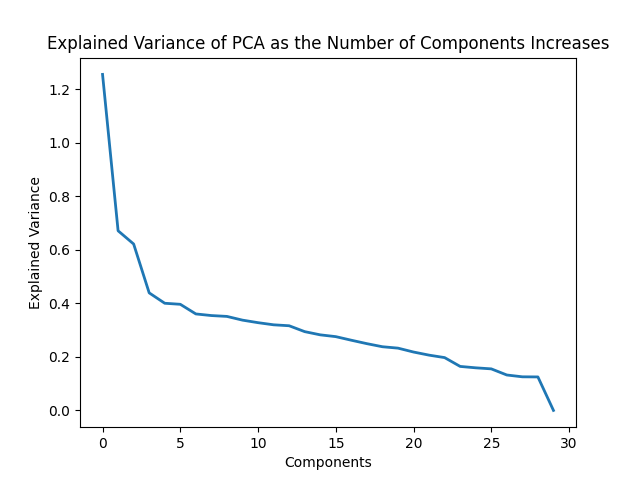
\includegraphics[scale=0.5]{my_agg/graphs/0_r0.png}
	\caption{Explained Variance with No Attacks at Round 0}
	\label{fig:pca_00}
\end{figure}
\\ \\
As seen in Figure \ref{fig:pca_00}, we can start to see that a dimension value of around one-four is probably the sweet spot.
Other rounds later on [\ref{fig:pca_01}, \ref{fig:pca_02}] may appear to indicate that actually we don't want to perform PCA at all.
However, this pattern only really appears when there are no attacks present and as soon as we start adding some, it becomes more apparent [\ref{fig:pca_50}] that this is not the case.
Instead, we end up seeing that a dimension value of one looks to be a pretty safe bet with some potential at rounds two-four.


\subsection{Low Dimensional Beings}
As has become apparent, relying on traditional methods to guarantee what the optimal values are, is not always the best idea.
So, to help further guarantee that the low PCA dimension values are correct, let's plot the coordinates of the PCA transforms of these values and see how they compare.
We can only do this in 1D, 2D, 3D and 4D but seeing as it theoretically shouldn't need to go beyond this anyway, it should be fine.
It should be noted that the 4th dimensions is represented by size of the plotted points in the graphs.
\\ \\
With no attacks you get pretty much what you would expect [\ref{fig:0mal_dims}] and all 4 dimensions show to add some level of useful information.
When we start adding attacks, we would expect that the most information gain happens from 1D and that is pretty much what you get at an initial glance.

\begin{figure}[htbp]
	\centering
    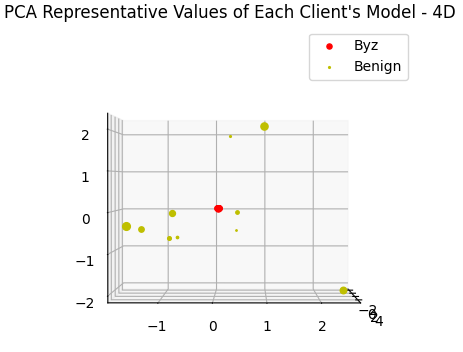
\includegraphics[scale=0.7]{my_agg/graphs/4d_diff.png}
	\caption{PCA Transform Positions in 4D, Alternate View - 20 Malicious - Round 0}
	\label{fig:4d_diff}
\end{figure}

As shown in Figures \ref{fig:5mal_dims} \& \ref{fig:20mal_dims}, we see that the remaining three dimensions all have the malicious clients placed in the middle of the same region [\ref{fig:4d_diff}] in their respective dimensions.
However, what becomes important is the scattering of the benign clients.
In all other dimensions they are far more unique, which lends them to not be clustered with the malicious clients even if the first dimension were to fail at separating the two groups.
This is also seen in practice, where the accuracy of 1D solutions tends to end up including more malicious clients as time goes on, showing that the segmentation isn't working as well as the Explained Variance would have you believe.

\begin{figure}[htbp]
	\centering
    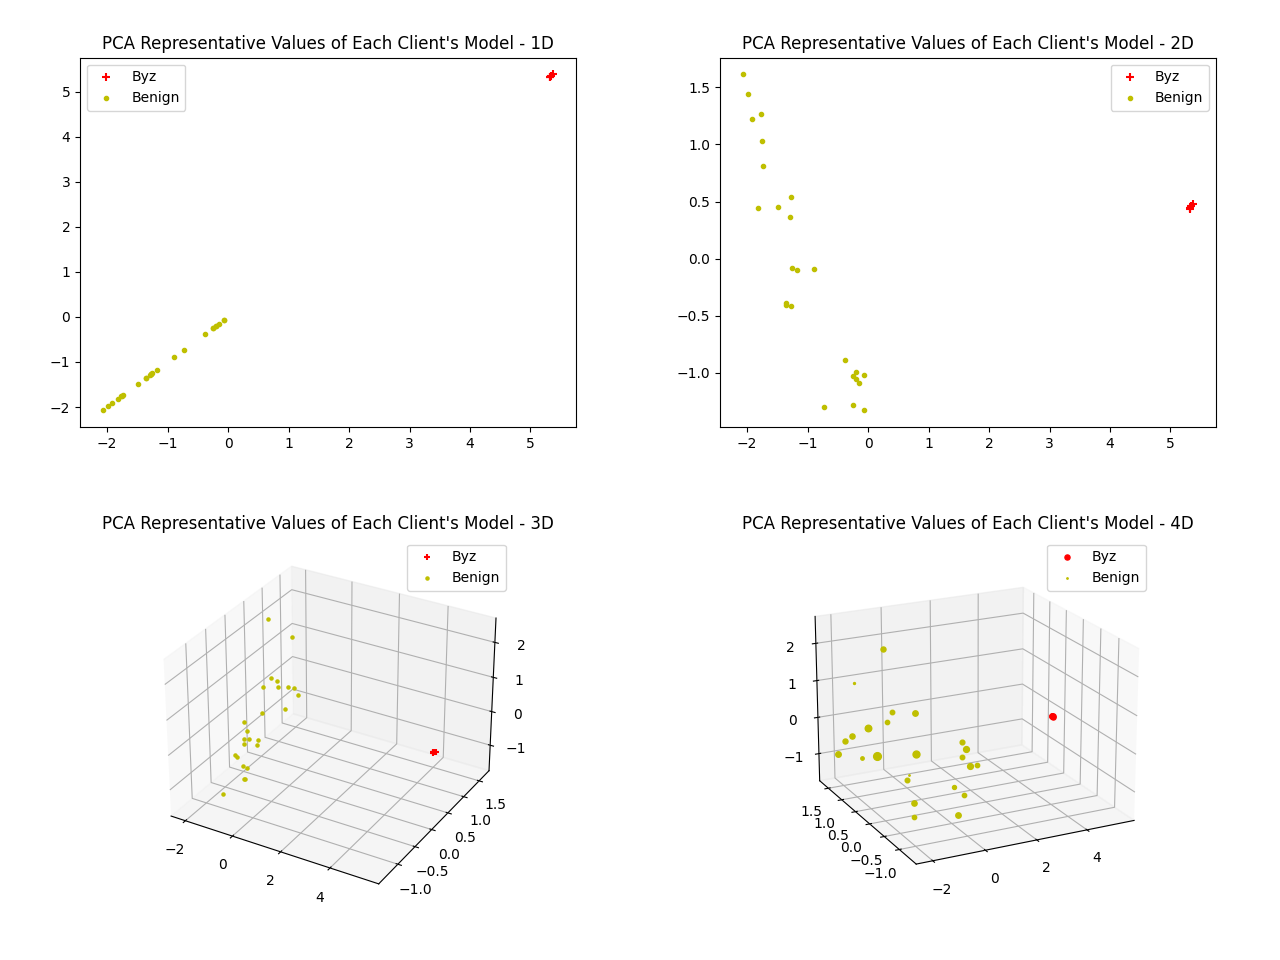
\includegraphics[scale=0.33]{my_agg/graphs/5mal_dims.png}
	\caption{PCA Transform Positions over Four Dimensions - 5 Malicious}
	\label{fig:5mal_dims}
\end{figure}
\\ \\
This is most likely due to the global aggregation sharing the global model out to every client, softening the malicious clients and making them appear more benign in the process.
This causes their PCA transform values to spread out more, increasing the likelihood that more clusters will be assigned to them.
This \textit{can} be mitigated through increasing the number of epochs per round (that's why 10 is used instead of two) but it isn't a perfect solution.
We are currently able to fix this through using four dimensions for the PCA but there is obviously something about 1D PCA that seems so tempting.
\\ \\
Increasing the number of dimensions doesn't really fix this and at higher dimensions (e.g. 10 [\ref{fig:dim10_26mal}] or 29 [\ref{fig:dim29_26mal}]) we still some spiking at later federated rounds.
The error rate is also not as smooth and is more susceptible to be jagged throughout, indicating that the current algorithm isn't as robust.



\section{Personalisation}
We nicely fall in the lap of federated learning personalisation.
We have hypothesised that the 1D PCA option might not be working as well simply because the malicious clients are getting good updates that makes them appear more benign over the course of the federated rounds.
This can be seen in Figure \ref{fig:mal_spread} as the spread is more segmented in 2D while in 4D there is only 1 dimension of spread that is much less segmented
So ideally, we don't want to give any malicious client a global update that will inevitably work against the benign clients.
\begin{figure}[htbp]
	\centering
    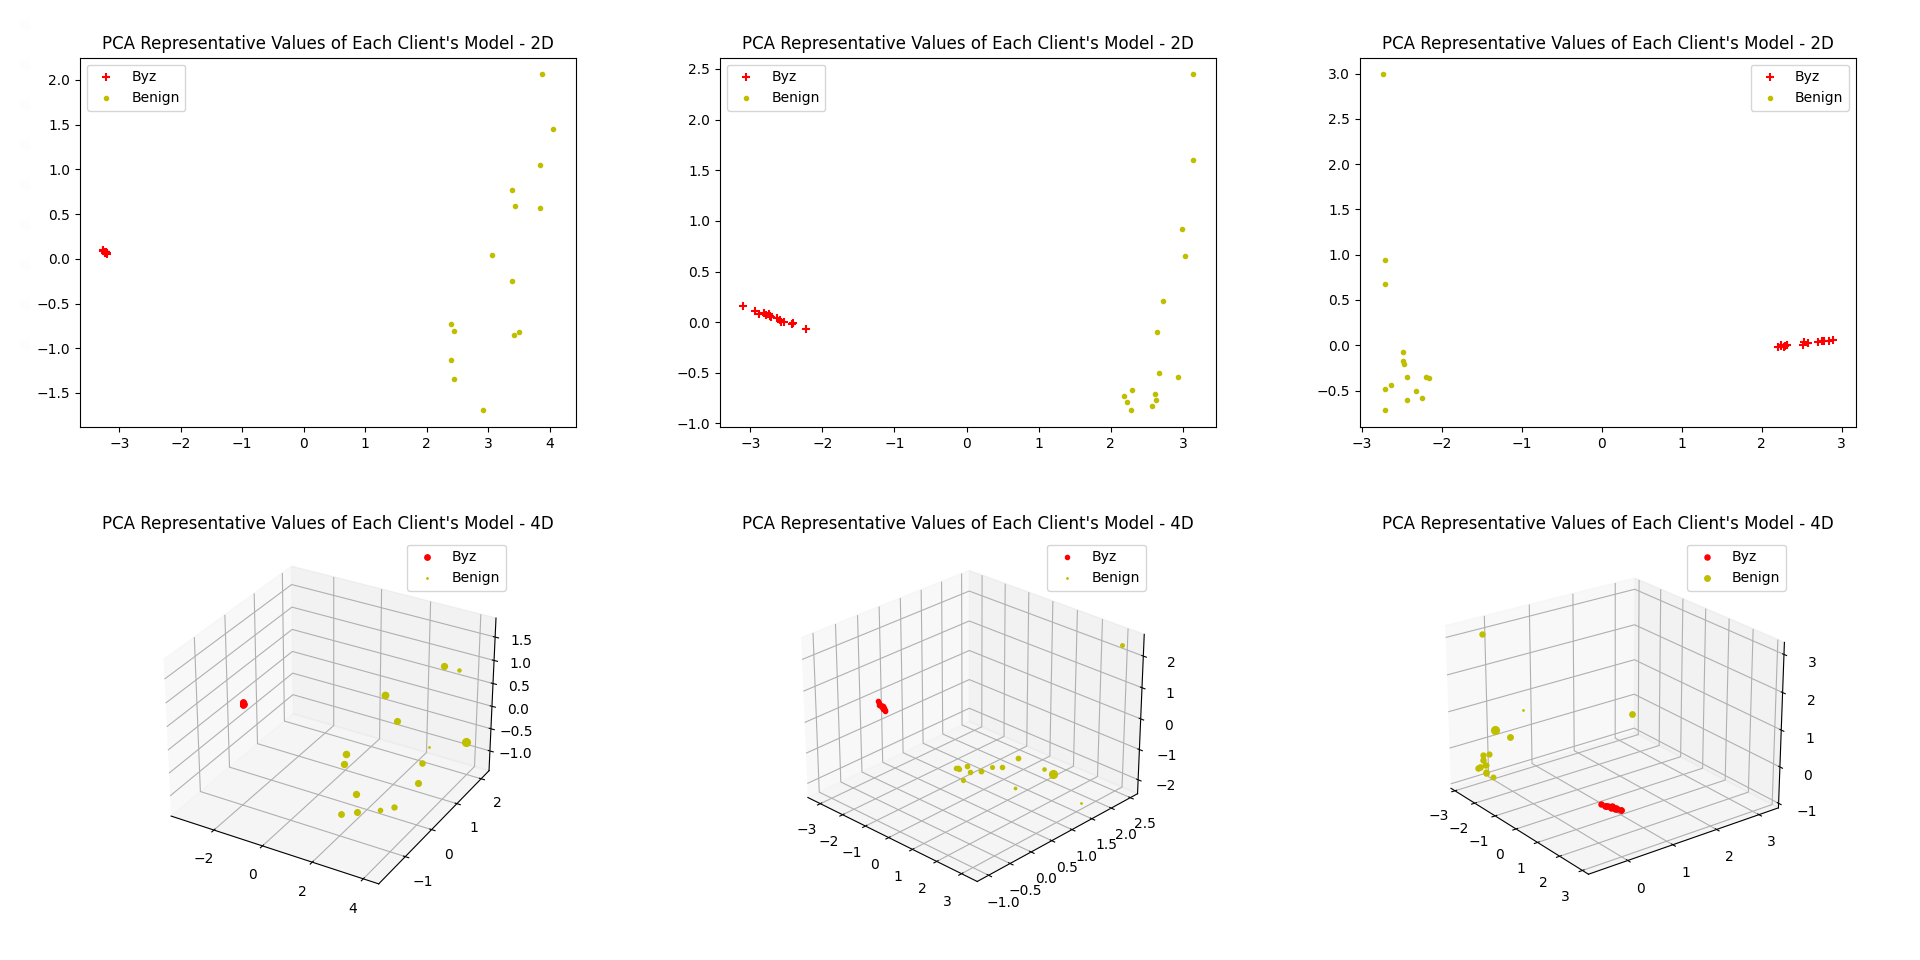
\includegraphics[scale=0.24]{my_agg/graphs/mal_spread.png}
	\caption{PCA Transform Position Spread for 2D (top) \& 4D (bottom) in Rounds 0, 1, 2}
	\label{fig:mal_spread}
\end{figure}
\\ \\
This is where the idea of personalisation comes in.
We either don't want to update certain clients or simply update them with less useful information that is specific to them.
This also gives us the capability to not have to use COMED to do the robust aggregation as we would already be robustly aggregating in the first place.
However, it may end up being more beneficial to also use COMED on top of this.



\subsection{Methods of Personalisation}
There are 4 main ways that I have come up with to achieve this, with the names that I will be using to refer to them as in the brackets:
\begin{enumerate}
    \item Selective Update (selective): this method involves only updating a select number of the clients at each round. This number would be determined by the floor of half of the number of clusters + 1. E.g. 3 for 5 clusters, 4 for 7, 5 for 9, etc. (we will assume 3 for K=5 from here on out).
    This would then hopefully lead to the malicious cluster not being updated (along with a benign one potentially) and the other clients in the selected clusters get an aggregated model of the top three clusters.
    \\ \\
    This would end up causing the main three clusters to get updated with data from each other, ultimately having them remain more similar and therefore more likely to update again together in later rounds.
    This would then help reduce the benign poisoning that is given to the malicious clients to help them.
    
    \item Concentrated and General Updates (general): here, we do two different global model updates.
    One is concentrated model of the top three best clients (as described above) and the other is a more general model from the aggregation of all of the clusters.
    Instead of just sending the concentrated model out to the best clients, it then gives the left-out benign cluster an opportunity to contribute to the other benign clusters later on, while still hopefully keeping the top 3 best clusters away from the malicious cluster.
    \\ \\
    This might not work as well, as the malicious client is still getting updated.
    There is also the possibility of then causing the best clusters to become too similar such that they merge and give a higher likelihood for the malicious clients to form more than one cluster.
    It will almost definitely cause the non-best benign cluster to then get polluted with damage from the malicious cluster as it will have received the general update which will include the malicious cluster in the aggregation.
    
    \item Thresholding (thresholding): instead of just using the best three out of five, instead we figure out which clusters are more than a set number of StDs away from the mean and then set their weighting to zero.
    This allows us to then aggregate on the rest of the data with their own personal weighting so that in theory, you get to fully aggregate on all of the benign clients' data, instead of just some of it.
    \\ \\
    This could also be applied in conjunction with the previous method such that the general model could then be aggregated on all non-zero weighting clusters while the concentrated model is still formed.
    You then also have the option to not update the zero-weight cluster at all like in the first method.
    
    \item No Global Model (no global): if we were to just not aggregate the clusters' models together, then in theory each client would get a more personalised model that was best suited to them.
    It would also keep all of the malicious clients building their own malicious model while all of the benign clients build their own separate ones.
    This would help minimise any form of cross-over between the clusters but it wouldn't allow for as much model generalisation.
    Depending on each client's end goal, this might not be an issue at all.
\end{enumerate}

Each method has its own strengths and weaknesses.
Although they can be used independently, it might be more beneficial to use some combination of them (as outlined in the Thresholding method) or to simply use just one sole method (like with the no global model option).


\subsection{Adaptive Weighting of Clusters}
To decide which clusters are deemed the ``best" and what weighting each cluster is given, there are 2 main scoring metrics for doing so.
One is in the form of Cosine Similarity and the other is a simple sum of squared differences between the parameter weights.
Seeing as the magnitude of the values in our data (the model parameters) matters, Cosine similarity might not be the best option as this isn't taken into account.
However, graphs of the PCA transform data do tend to put the benign clients' values on a similar angle to each other and so it may still be a suitable metric.
\\ \\
To do either of these methods, you need to have a starting point as a point of reference to do the calculations from.
So, for every cluster, I calculate the scoring metric relative to that cluster so that I end up with a 2D 5x5 grid of values.
To find the ``best" clusters, I proceed to then take the best three scores from each list and sum them together.
Which ever the max value is, I take the according list of values, normalise them, and then use those for the weights.
This leaves me with a set of weights where I have the three ``best" clusters being the closest/most similar options.
After this has taken place, I can then follow through the rest of the algorithm according to which method of personalisation I choose.
The pseudocode for this is outlined in Algorithm \ref{alg:my_alg}.
\\ \\
This weighting algorithm is used in all of the first three methods and is crucial in deciding the best models to choose from.
One part on Line 36 should be noted as maybe not being a solution that should be incorporated every time.
In the instance where a malicious cluster is being used in aggregation when it shouldn't be, where there are a lot of malicious clients, this weighting could cause much more drastic effects than without it.
\\ \\


\begin{algorithm}[htbp]
\SetAlgoLined
\DontPrintSemicolon
\SetKw{KwIn}{in}
\SetKw{KwMath}{maths}
\newcommand\mycommfont[1]{\footnotesize\ttfamily\textcolor{blue}{#1}}
\SetCommentSty{mycommfont}
 import \KwMath\;
 \;
 \tcc{Some initial starting values}
 cluster\_count = 5\;
 num\_to\_take = \KwMath.floor(cluster\_count / 2) + 1\;
 cluster\_weights = generate\_weights(self.cluster\_centres)\;
 distances = [[] for \_ in range(cluster\_count)]\;
 \;
 \tcc{Calculating the distance between each cluster centre and every other cluster}
 \For{i, m1 \KwIn enumerate(cluster\_weights)} {
  \For{j, m2 \KwIn enumerate(cluster\_weights)} {
   d = (m1 - m2).square().sum()\;
   distances[i].append(d)\;
  }
 }
 \;
 best\_dist = \KwMath.infinity()\;
 best\_indices = []\;
 best\_i = -1\;
 \;
 \tcc{Calculating the best cluster centre that should be used for distance choice}
 \For{i, dist \KwIn enumerate(distances)} {
  indices = n\_smallest(num\_to\_take, dist)\;
  total\_dist = sum(dist[i] \textbf{for} i \KwIn indices)\;
  \;
  \If{total\_dist $<$ best\_dist}{
   best\_dist = total\_dist\;
   best\_indices = indices\;
   best\_i = i
  }
 }
 \;
 \tcc{Calculating weigths to use for each cluster}
 weights = [w / sum(dists[best\_i]) \textbf{for} w \KwIn dists[best\_i]]\;
 weights = 1 - weights\;
 weights /= weights.sum()\;
 \;
 std = \KwMath.std(weights)\;
 mean = \KwMath.mean(weights)\;
 cutoff = mean - std\;
 \;
 best\_models = [self.cluster\_centres[i] \textbf{for} i \KwIn best\_indices]\;
 weights[weights $<$ cutoff] = 0\;
 \tcc{Resizing weights so that bigger clusters get a more proportionate weight}
 weights *= size\_of\_each\_cluster\;
 weights /= weights.sum()\;
 \;
 \textbf{return} best\_models, weights, best\_indices\;

 \caption{FedPADRC Exterior Aggregators' Clustering Weight Calculation}
 \label{alg:my_alg}
\end{algorithm}

\section{Evaluation}
Looking back at the goals of what I wanted to achieve, it has so far become apparent that I have been able to do them all with the current exception of detection of free-riders.
Hopefully looking at how the various forms of personalisation perform, this goal shall also be met.
\\ \\
To recap, I also wanted to achieve better aggregation through personalisation for 1D PCA as well as in general and so I will be initially testing that.
I tested selective, general, selective with thresholding, general with thresholding and no global as forms of personalisation.

\subsection{4D Personalisation}
I made sure to try with 4D PCA first, so as to make sure that I wasn't going to be losing any performance with the discussed methods.
There was also the need to test both COMED and FedAvg at both levels of aggregation, as this would hopefully lead to being able to not need COMED to do the robust aggregation and then hopefully purely relying on personalisation techniques.
This would enable greater generalisation capabilities that would hopefully allow more non-IID data to be aggregated better.
\\ \\ 
With COMED, we saw typically really good performance with the clients only starting to fail with use of the general method under 24 malicious clients [\ref{fig:4d_24mal}].
With FedAvg, we see the same level of performance with the selective methods but under general, the no thresholding method fails pretty quickly at five malicious clients [\ref{fig:4d_5mal}] while the thresholding method fails at around 15 [\ref{fig:4d_15mal}].
This makes me realise that the general method is one that just doesn't perform to the same standard as without personaliation.
\\ \\
This is most likely because with general, we are still updating the malicious clients with a model, even if it is not as good as the selective model.
It can also cause the benign client that isn't participating in the selective update to become more similar to that of the malicious clients, causing there to be increased chances of leakage.
This is even without the fact that with no thresholding, you are then still just aggregating with the malicious clients at every step, and so nothing too robust is even happening.
Therefore, proceeding with the general method for 1D would be futile and so won't be considered further.



\subsection{1D Personalisation}
Once I removed the generalisation from the testing, with both COMED and AFA I got pretty much the same results across the board.
Through all levels of malicious clients, with and without thresholding, the selective method held up throughout [\ref{fig:1d_26mal}].
This was great to see as this was a great win in terms of being able to use FedAvg for the aggregation instead of COMED, allowing greater data use.
\\ \\
This helps definitively prove that personalisation helps with the robustness of the algorithm and as such, should be treated as an essential part of the process.


\subsection{No Global}
As much as has been shown that the selective method works well, what if there were more than one attack or more than one type of attack present?
In this case, it may end up being the case that you don't want to do any aggregation amongst the clusters at all for the fear of being damaged from too many angles.
\\ \\
This is where the no global method shines.
It is essentially a more strict version of the selective algorithm in that there is only aggregation taking place within each cluster and not between the clusters themselves.
This allows for each cluster to independently perform without the worry of other clusters affecting its performance.
\\ \\
This works well in either 4D or 1D PCA with the sole difference being that at 26 malicious clients there are temporarily two clusters that contain malicious clients before eventually all of the malicious clients form into one cluster.
This is shown in Figure \ref{fig:1D_no_global} where each line represents a different cluster.
\begin{figure}[htbp]
	\centering
    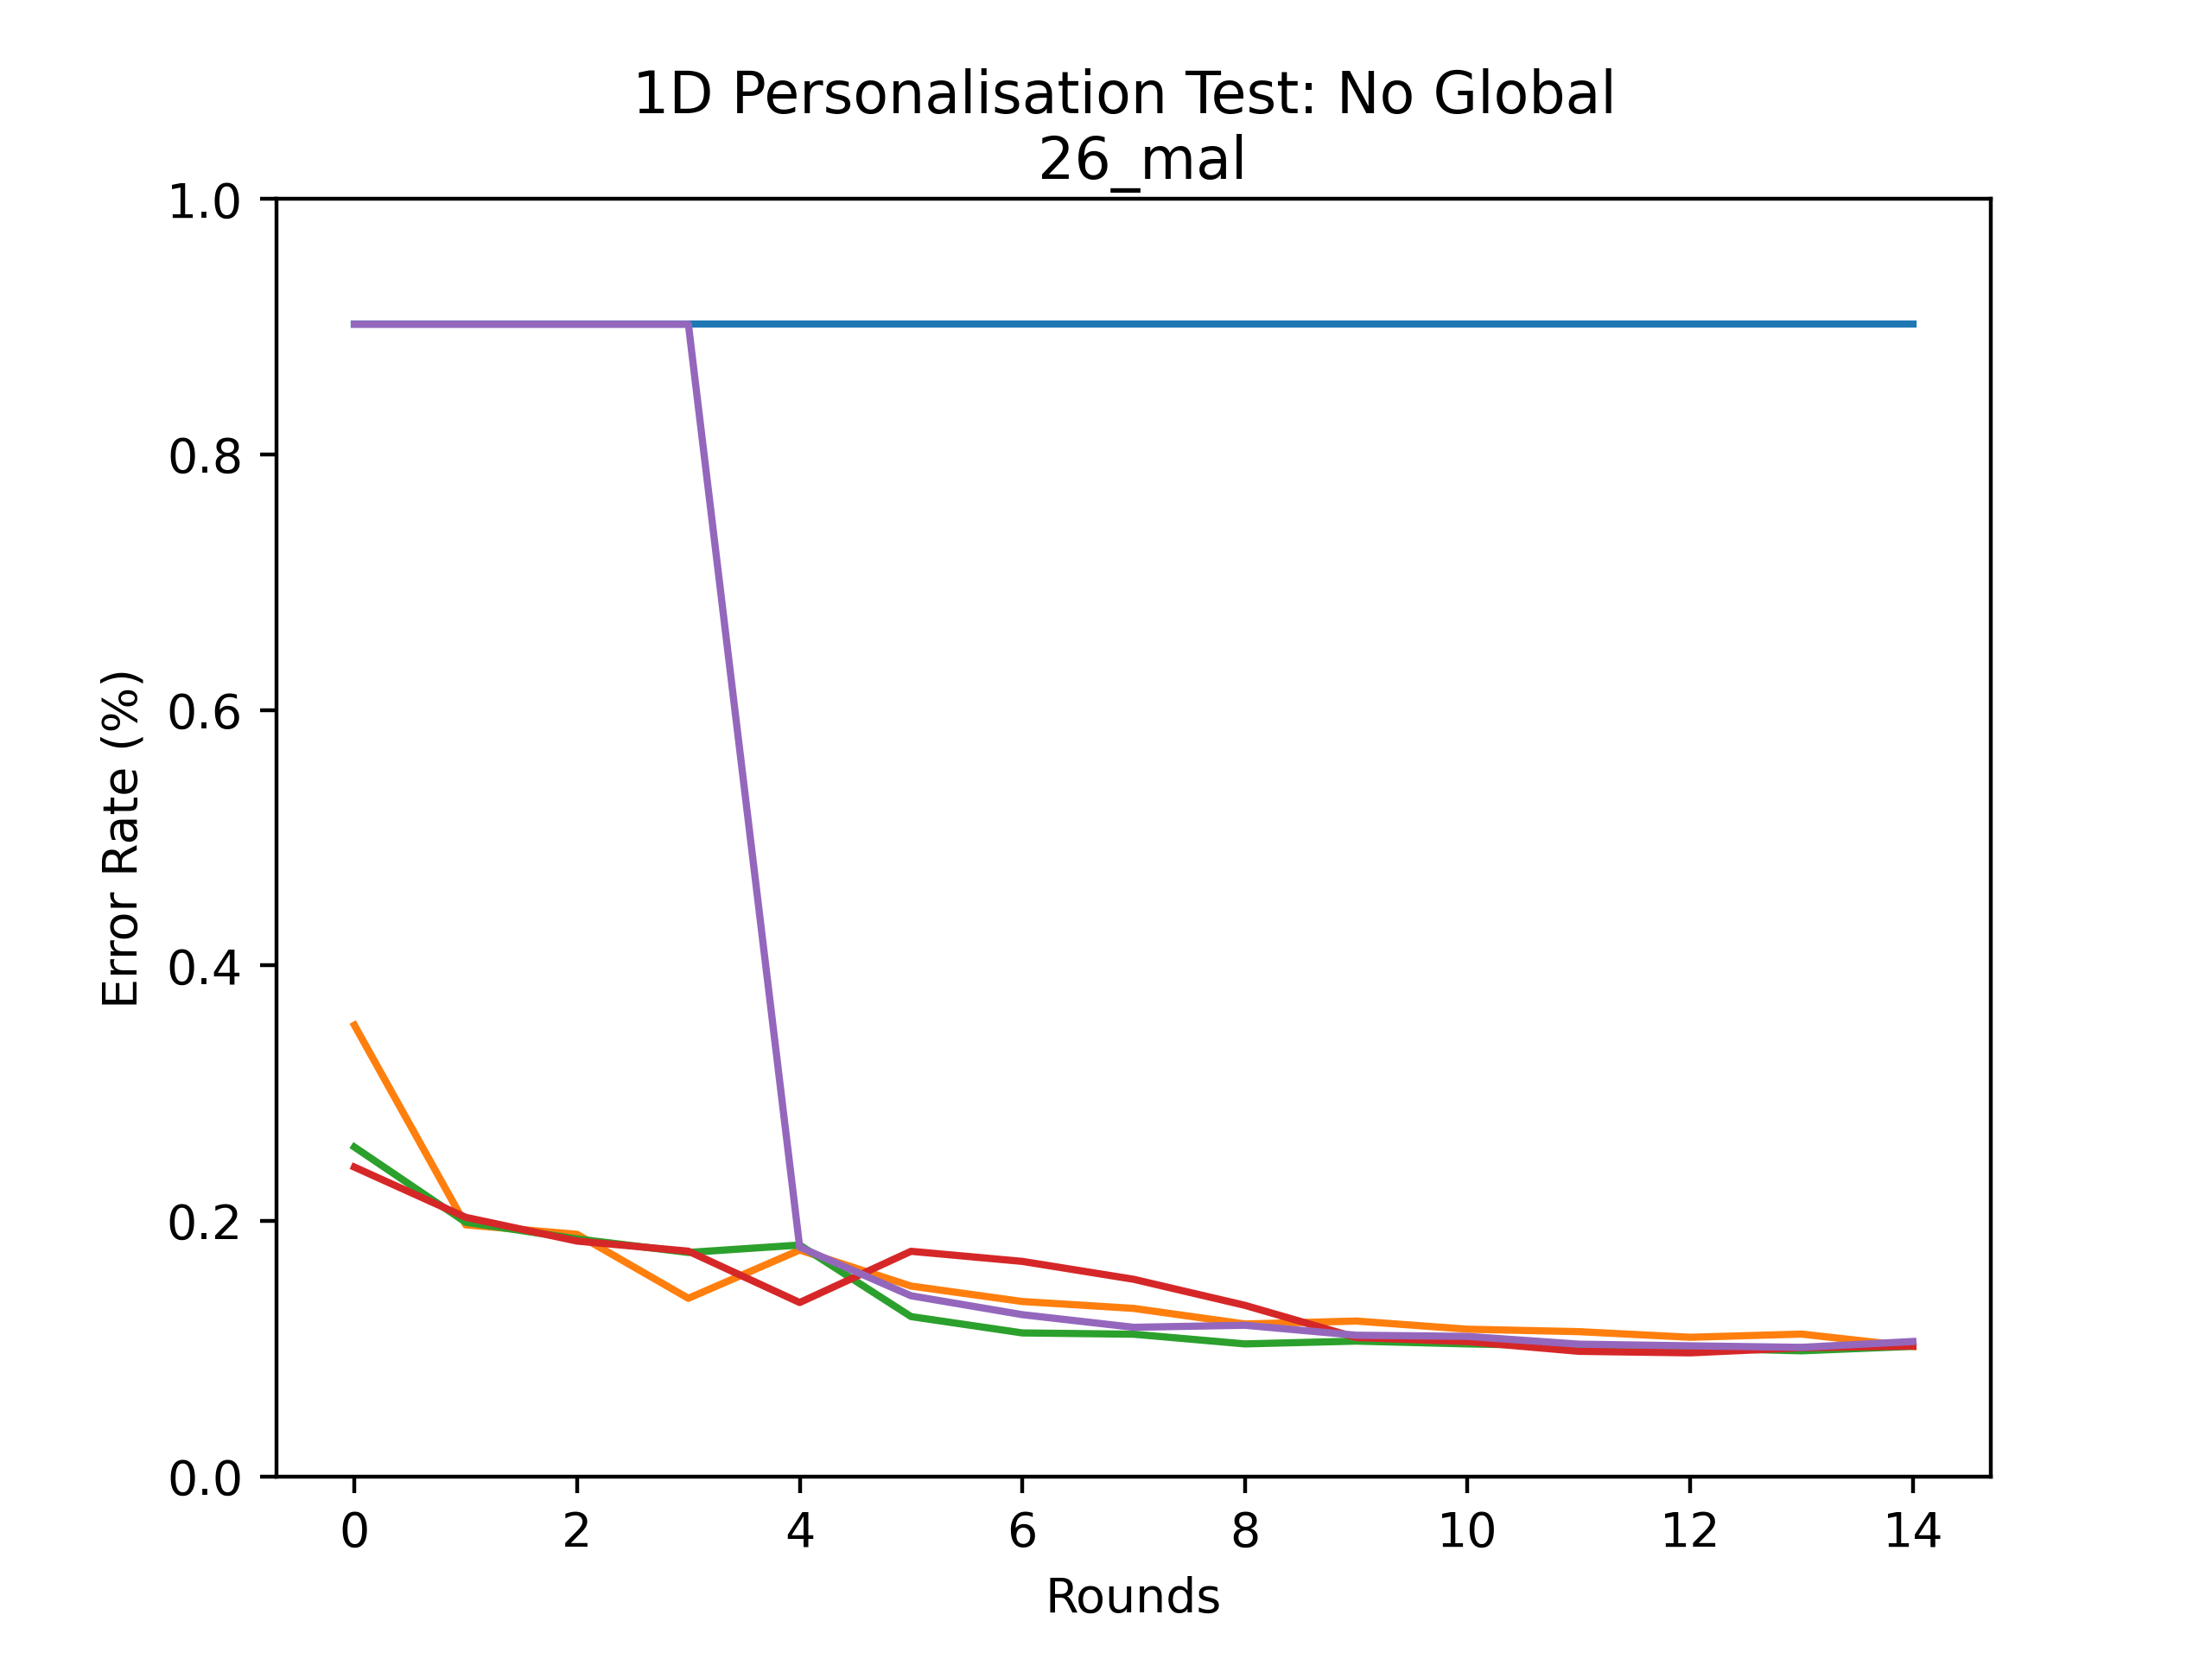
\includegraphics[scale=0.5]{my_agg/graphs/1d_no_global.png}
    \caption{1D PCA with the No Global Personalisation Method - 26 Malicious Clients}
	\label{fig:1D_no_global}
\end{figure}
The great thing about this is that this works at any level of malicious clients [\ref{fig:4D_no_global_1}] with the only noticeable difference being the random spikes that are caused because the labels assigned to clusters change.
It should be noted as well that the malicious clusters only ever contained malicious clients and the benign clusters only ever contained benign clients.
As such, there was no overlap or poisoning at all, not even by a single client.

\subsection{Free-Riders}
The final step in achieving all that was set out to do is to help conquer the free-riders.
The two options that are present are the no global method and the selective method.
\\ \\
For no global, the hope is that all of the free-riders will group together into their own cluster (due to their similarity) and will then not receive any contributions from proper clients.
Or at the very least, not get a properly converged model.
This might be harder due to the nature of the free-riders, and a few benign clients might be lost in the process if they get caught up in the same cluster as the free-riders.
\\ \\
For the selective method, it might be harder but the goal is to have the free-riders be in one of the two left-out clusters.
This allows for some leniency hopefully but at the same time there is more risk associated with that there is an increased chance of them stealing a good model if they are included in the selected group.
Either way, seeing how FedPADRC handles free-riders by itself as well as with malicious clients is what I shall test.
\\ \\
The no global method is the first testing point as if it can't work here, then it won't be able to handle the more lenient selective method.
I am also doing the testing with 4D PCA just to make sure that it isn't that causing any potential problems.
\\ \\
What ends up occurring is something quite magical and yet so obvious!
The free-riders get the same global model that is sent out at the very start of the process but they can't really make any realistic changes to it.
Therefore, every other client (whether or not it is malicious) will do some form of learning.
This then has a great distinctive effect of having the free-riders all look the same [\ref{fig:10mal10free_rep}] \textit{as well as} not being similar in any shape or form to the rest of the clients.
As such, it never even gets the opportunity to learn even a little bit, meaning that the free-riders fail in their goal [\ref{fig:no_15free}] as well as there being no intellectual property theft.
What's also good is that there wasn't even 1 free-rider that managed to sneak into the other clusters at any count of free-riders, they remained separate at all times.

\begin{figure}[htbp]
	\centering
    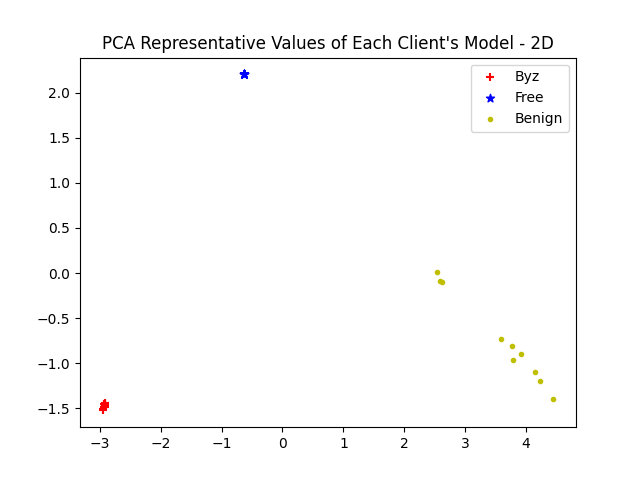
\includegraphics[scale=0.5]{my_agg/graphs/10mal_10free_r0_no_global.png}
    \caption{2D PCA Transform Representation with the No Global Personalisation Method - 10 Free, 10 Malicious at Round 0. This shows the separation of the clusters even when there are a combination of malicious and free-riding clients.}
	\label{fig:10mal10free_rep}
\end{figure}
\\ \\
It might end up being the case that FedPADRC isn't able to handle more than just one style of attack at any given time.
Alas, that is not the case!
Even when there is a combination of free-riders and malicious clients present [\ref{fig:no_13free_13mal}], it is not hindered in any-way-shape-or-form.
All that then happens is that there are two clusters that have awful performance with the three benign clusters making up all of the remaining benign clients.
\begin{figure}[htbp]
	\centering
    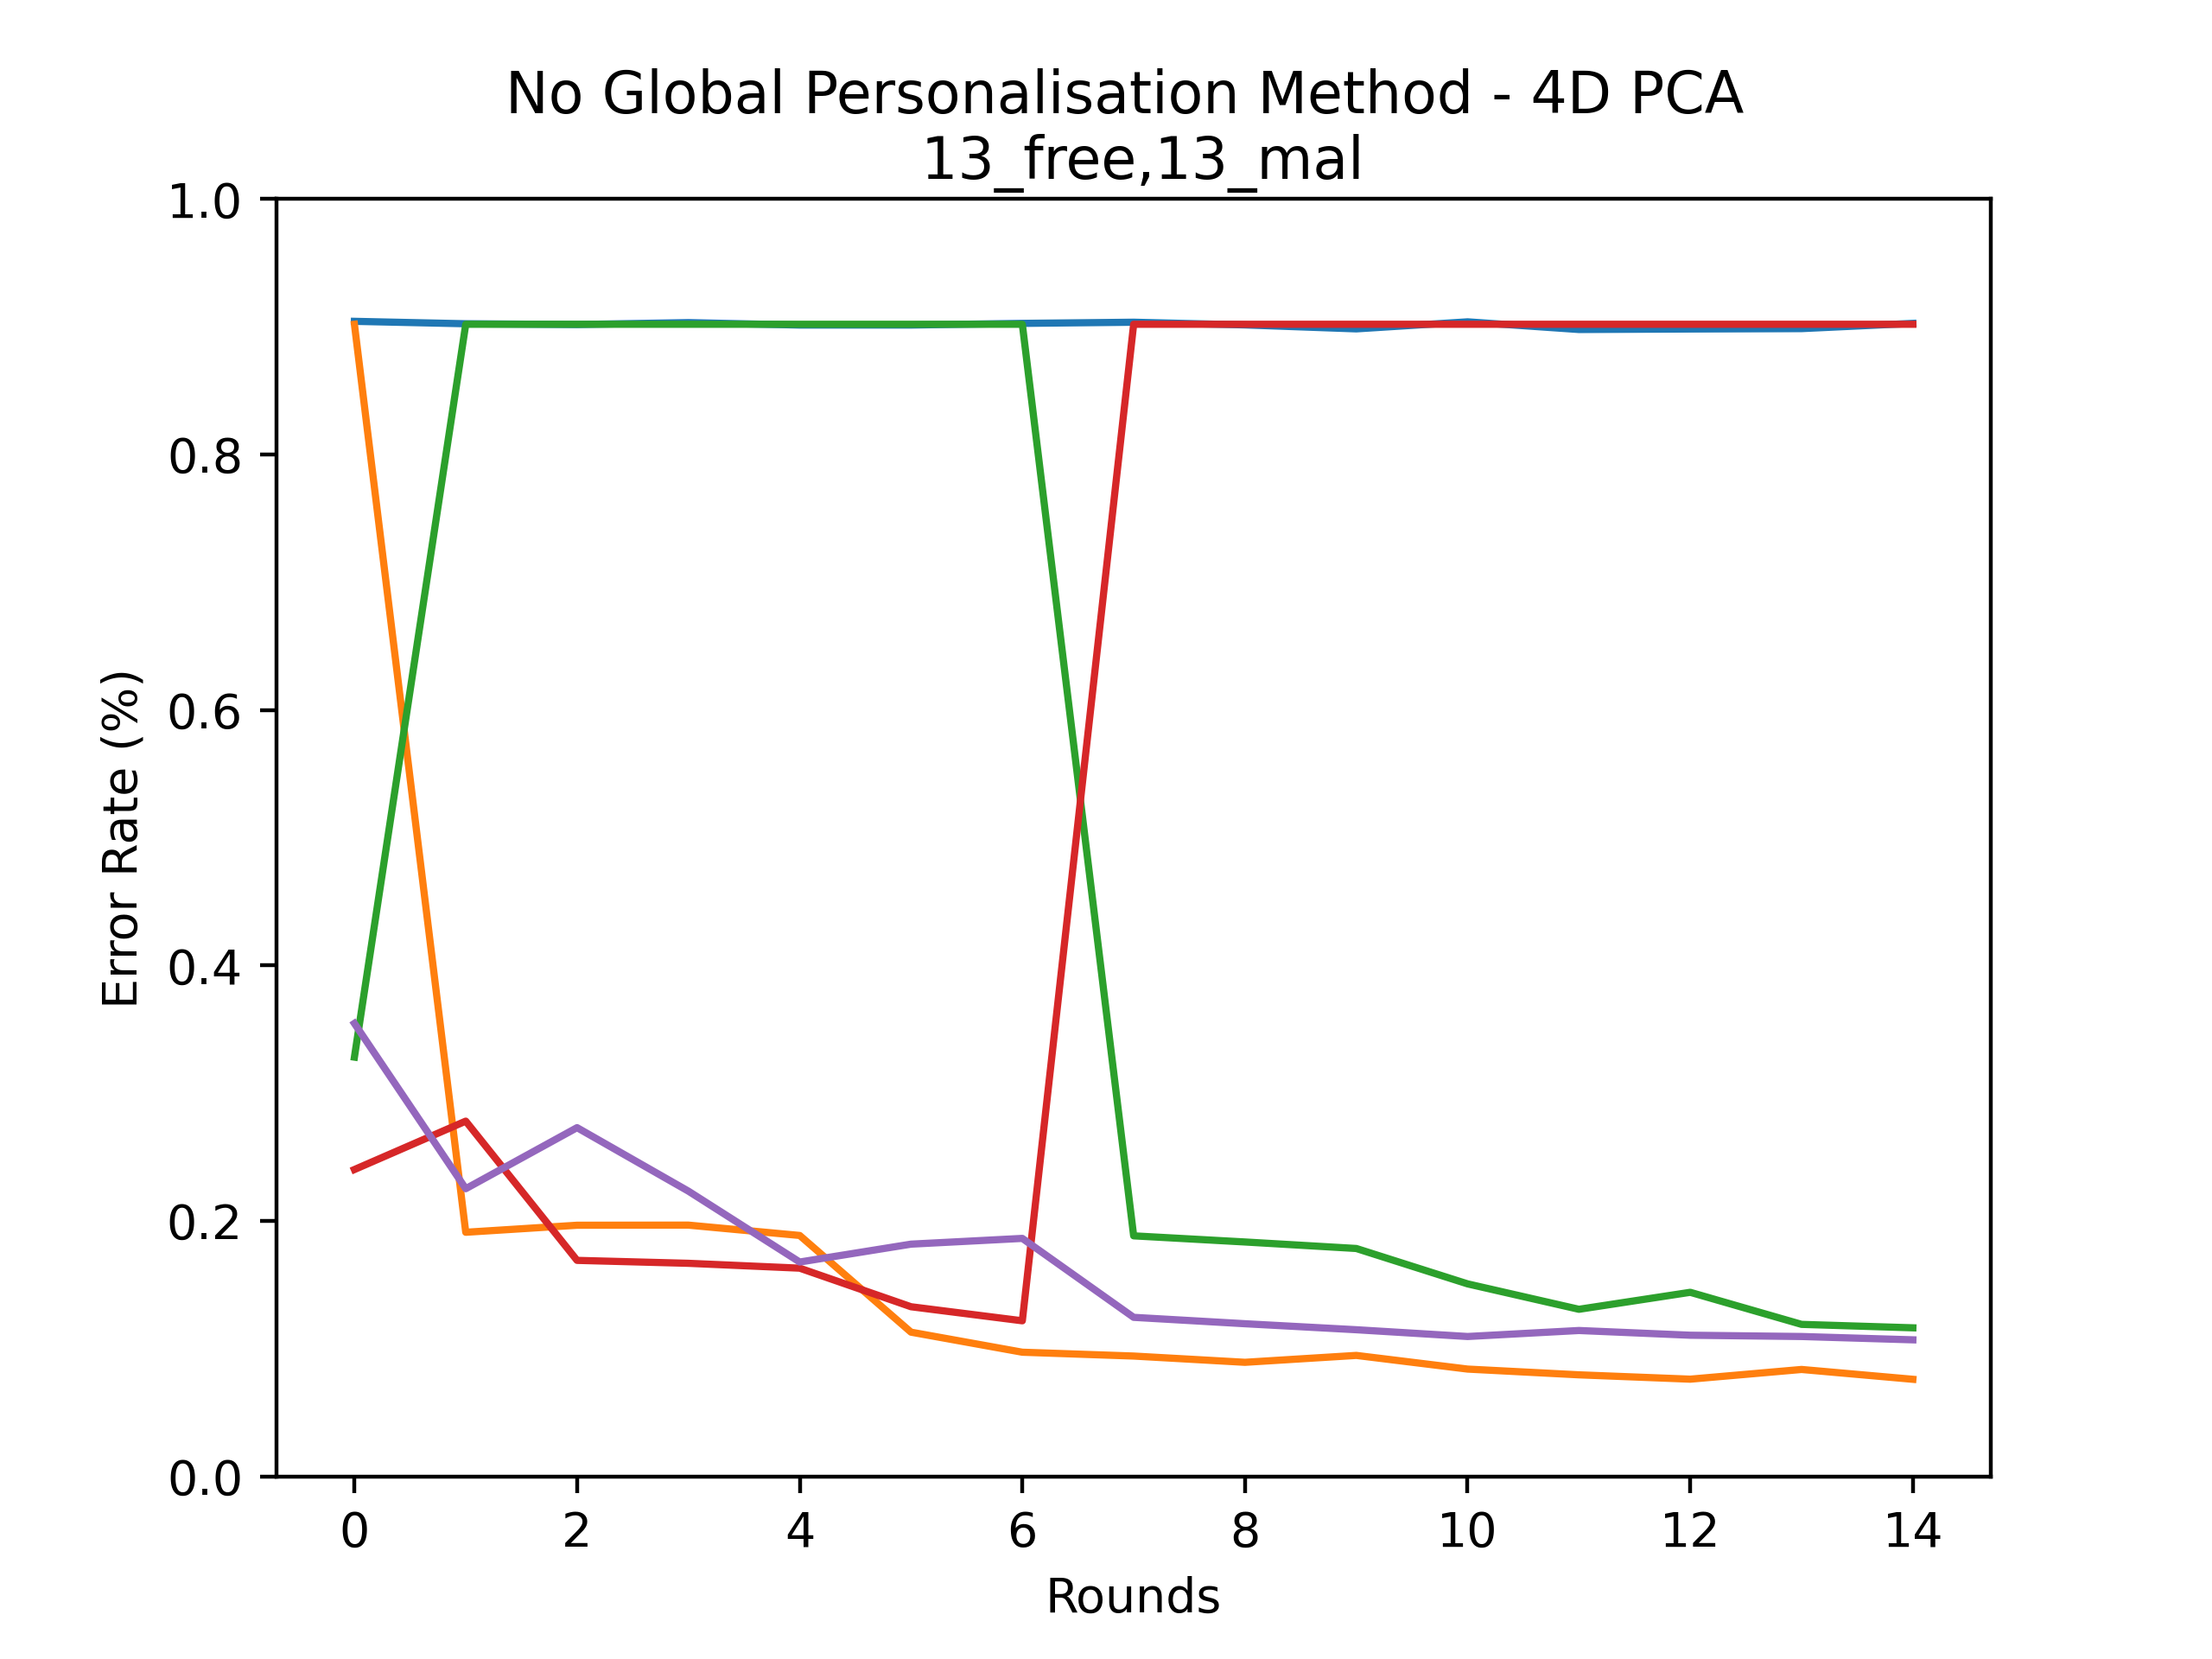
\includegraphics[scale=0.5]{my_agg/graphs/no_global_13free_13mal.png}
    \caption{4D PCA with the No Global Personalisation Method - 13 Free and 13 Malicious Clients. This shows that even under a combination attack, FedPADRC is able to hold its own.}
	\label{fig:no_13free_13mal}
\end{figure}
\\ \\
All of the above results are also emulated with the selective personalisation method.
This allows for the configurator of the federated system to be a bit more strict or lenient with the aggregation setup, allowing more variability for ensuring the robustness of the aggregation.



%%%%%%%%%%%%%%%%%%%%%%%%%%%%%%%%%%%%
\chapter{Conclusion and Future Work}
\section{Conclusion}
This project, in its entirety, has achieved the goals that it set out to do as outlined in the introduction and in the beginning of Chapter \ref{chap:fedpadrc}.
Evaluation was done on all of the current most popular forms of robust aggregation, leading to being able to make additional enhancements made to FedMGDA+.
Accuracy improvements and robustness of FedMGDA++ was discussed and shown with more noticeable improvements made to capability of blocking.
It went from blocking five clients (three benign and two malicious) to blocking all of the malicious clients and no benign ones with eight malicious clients.
It also allowed for a smoother learning process and higher numbers of malicious clients being handled, up to around 11 malicious clients.
\\ \\
We also saw how free-riders were able to absolutely smash past all robust aggregators and prove incapable of being detected by traditional means.
This further proved the need for a robust aggregator that was more capable of handling the federated domain.
\\ \\
Through clustering, this project proved that robust aggregation methods like COMED could be significantly enhanced to be able to handle up to around 22 malicious clients well, far surpassing that of any other solution currently available.
Further work was then done to strengthen the robustness of the algorithm through dimension reduction with PCA before finally optimising the performance with personalisation methods.
We saw up to 26 malicious clients being easily handled by our variety of FedPADRC configurations as well as handling free-riders in a way that no other previous solution could.
It should be noted that 26 is somewhat of a theoretical limit with K=5 K-Means Clustering, due to having any fewer benign clients would automatically assign more than one cluster to the malicious clients.
\\ \\
All-in-all, all goals that were met were comfortably done so.
We also provided a robust aggregator that has been shown to be the best performing under the given attack strategies as well as being a more robust algorithm as a whole.

\section{Future Work}
There are many ways in which this project could be extended if time permitted.
I will end this project with a few ways that I have thought of in which the work done could be taken further.

\subsection{Non-IID Data}
Throughout this project, the main focus has been on IID data.
This is because Federated Learning naturally has problems when trying to aggregate on this type of data and so it would interfere with the type of testing we were doing.
\\ \\
That does not mean that it is not extremely important to consider though.
Several methods already exist for non-robustly aggregating on non-IID data (e.g. FedMA, Auto-FedAvg) but the space for non-IID aggregation for robust aggregators is more limited.
This is because it forms an even trickier problem to handle.
If we have a variety of aggregators basing their aggregation on anomaly detection, it could very well come to pass that certain clients with odd distributions of data do not make the cut.
This would hinder the generalisability of the global model as crucial data could be being left out.
Even ignoring anomaly detection, certain aggregators like COMED would only be sampling from such a small amount of clients that it would without-a-doubt not be able to cover the entire space of data that is being handled.
\\ \\
When it comes to clustering, a different problem is faced altogether.
You could have clients that hold labels 1, 2, 3 and others that hold only 7 and 8.
This would lead to clusters forming around these similar clients.
This is not necessarily a bad thing if the model that these clients are after is highly personalised, but with the selective method of personalisation, you would be leaving out potentially entire labels of data.
This might lead to further fine tuning and investigation needed into the generalisation method of personalisation in making it more robust so as to be able to handle these non-IID cases.
Having a more distributed data space would also increase the likelihood of the malicious/free-riding clients to be included with other benign clients and clusters, breaking the robustness of the model.
Investigations into the use of higher K-values for clustering might be needed here.

\subsection{Label Flipping Attacks}
The attack that was used throughout this project was setting the malicious clients' labels to be all zero.
It would be worth investigating the effects of changing this attack to be something more subtle such as changing 3s and 8s around.
This might mean that the malicious clients end up appearing more benign to FedPADRC or it could be that they're still different enough for it to pick up on.
This could also be paired with multiple different pairs of flipping e.g. 2 and 5, 3 and 8, 8 and 0 etc.
This might prove harder for clustering strategies to then group them into their individual clusters by themselves.
However, if there is overflow into benign clusters, the use of COMED instead of FedAvg at the internal aggregator level could be used to help further mitigate this overflow.
\\ \\
Another style of attack that was not looked into as rigorously was untargeted attacks.
Here, we could randomly flip all the labels or offset them all by one in such a way that it causes non-specific havoc.
This would probably be a fairly noticeable attack to several of the robust aggregation strategies, but it would not at least be specific for any given label.


\subsection{Local Test Data}
In most federated learning solutions, clients do not test/validate their data locally to see how it performs.
Even when they do, it's more for a personal scoring metric, that might be used in something like personalisation, to help them individually.
What would be more interesting is if the local clients sent their validation performance to the central server along with the model update.
The reasoning behind this is that if you are a malicious client, you are faced with three options:
\begin{enumerate}
    \item Have the validation dataset have all of its labels also set to 0.
    In this case the malicious clients will initially end up with an exceedingly high accuracy compared to the other clients, which would be suspicious.
    As the aggregation carries on, the malicious clients will have their performance degrade (if they do not overpower the system) as they gain more influence from the benign clients' model aggregation.
    This would be quite an anomaly to see the performance degrade and so might be a way to highlight malicious clients.
    
    \item Use the original validation set that has not been tampered with.
    In this case, the initial performance would be rock-bottom, leading to a potentially very-low assigned weight.
    This would then cause either blocking or for minimal effect to occur on the aggregation, ultimately looking like a big anomaly from the get-go.
    
    \item Lie about the validation accuracy with some strategy behind the updated scores.
    This would then involve prior knowledge of the system and the other clients to be able to make assumptions on how they will perform to blend in.
    This might be possible based on the network used, the LR and other parameters.
    However, no client would see any other client's score and would only be getting a global model update, not an individual one from each client.
\end{enumerate}

As you can see, all three methods outlined have their issues and so further investigation could prove fruitful in terms of robustly aggregating.


\subsection{Block and Rerun}
This is a rather simple idea but it is based on the fact that both AFA and FedMGDA++ end up blocking all of the malicious clients even when they no longer work (> 11 malicious clients).
This leads to an idea where the whole federated solution is run once initially to see which clients get blocked and then run again (potentially with a different aggregator) but without the blocked clients.
There then would not be the problem of having to worry about malicious clients as much, and it would leave room for higher number of malicious client attacks to be able to be robustly aggregated against.


\subsection{Medical Data}
Ideally FedPADRC should get tried and tested more thoroughly with more proper datasets such as medical ones.
This is to just help ensure that it works better in the real-world and not just with MNIST.


%%%%%%%%%%%%%%%%%%%%%%%%%%%%%%%%%%%%
\chapter{Ethical Issues}
There are three points in the ethical consideration table [\ref{tbl:ethical-table}] that might be necessary to cover:
\begin{itemize}
    \item Personal data processing
    \item Sensitive personal data processing
    \item Previously collected personal data processing
\end{itemize}
Every one of these points is due to the inclusion of datasets that are used to train Machine Learning models to test the Federated Learning techniques discussed in this paper.\\ \\
These are in the form of the MNIST dataset that is publicly available for anyone to use. 
For this data we do not have any identifiable information about any of the images and so it isn't personal in any way.
\\ \\
This then doesn't leave me with any ethical considerations as I don't need to worry about storing, sending, processing or any form of handling of this data as it is a public dataset with nothing that ends up being sensitive or personal. 
The participants involvement in the original data collection are then no longer relevant in the use of the data by other individuals and so no longer need to be considered.
\\ \\
However, I do just note them down as potential points of consideration for future work that might be undertaken with the work that I have contributed in this project.

%%%%%%%%%%%%%%%%%%%%%%%%%%%%%%%%%%%%
%% bibliography
\bibliographystyle{unsrtnat}
\bibliography{references}

%%%%%%%%%%%%%%%%%%%%%%%%%%%%%%%%%%%%
\begin{appendices}
\chapter{Ethical Consideration Table}
\begin{center}
    \begin{longtable}{ | m{30em} | m{1.5em} | m{1.5em} | }
    \caption{Ethical Consideration Table}
    \label{tbl:ethical-table}
    \hline
    & Yes & No \ \\ \hline
    \cellcolor[HTML]{C0C0C0} Section 1: HUMANS &  & \  \\ \hline
    Does your project involve human participants? &  & x \\ \hline
    \cellcolor[HTML]{C0C0C0} Section 2: PROTECTION OF PERSONAL DATA &  & \  \\ \hline
    Does your project involve personal data collection and/or processing? & x &  \\ \hline
    Does it involve the collection and/or processing of sensitive personal data (e.g. health, sexual lifestyle, ethnicity, political opinion, religious or philosophical conviction)? & x &  \\ \hline
    Does it involve processing of genetic information? & & x  \\ \hline
    Does it involve tracking or observation of participants? It should be noted that this issue is not limited to surveillance or localization data. It also applies to Wan data such as IP address, MACs, cookies etc. & & x  \\ \hline
    Does your project involve further processing of previously collected personal data (secondary use)? For example Does your project involve merging existing data sets? & x &  \\ \hline
    \cellcolor[HTML]{C0C0C0} Section 3: ANIMALS & & \  \\ \hline
    Does your project involve animals? & & x  \\ \hline
    \cellcolor[HTML]{C0C0C0} Section 4: DEVELOPING COUNTRIES &  & \  \\ \hline
    Does your project involve developing countries? & & x  \\ \hline
    If your project involves low and/or lower-middle income countries, are any benefit-sharing actions planned? & & x  \\ \hline
    Could the situation in the country put the individuals taking part in the project at risk? & & x  \\ \hline
    \cellcolor[HTML]{C0C0C0} Section 5: ENVIRONMENTAL PROTECTION AND SAFETY &  & \  \\ \hline
    Does your project involve the use of elements that may cause harm to the environment, animals or plants? & & x  \\ \hline
    Does your project involve the use of elements that may cause harm to humans, including project staff? & & x  \\ \hline
    Section 6: DUAL USE &  & \  \\ \hline
    Does your project have the potential for military applications? & & x  \\ \hline
    Does your project have an exclusive civilian application focus? & & x  \\ \hline
    Will your project use or produce goods or information that will require export licenses in accordance with legislation on dual use items? & & x  \\ \hline
    Does your project affect current standards in military ethics – e.g., global ban on weapons of mass destruction, issues of proportionality, discrimination of combatants and accountability in drone and autonomous robotics developments, incendiary or laser weapons? & & x  \\ \hline
    \cellcolor[HTML]{C0C0C0} Section 7: MISUSE &  & \  \\ \hline
    Does your project have the potential for malevolent/criminal/terrorist abuse? & & x  \\ \hline
    Does your project involve information on/or the use of biological-, chemical-, nuclear/radiological-security sensitive materials and explosives, and means of their delivery? & & x  \\ \hline
    Does your project involve the development of technologies or the creation of information that could have severe negative impacts on human rights standards (e.g. privacy, stigmatization, discrimination), if misapplied? & & x  \\ \hline
    Does your project have the potential for terrorist or criminal abuse e.g. infrastructural vulnerability studies, cybersecurity related project? & & x  \\ \hline
    \cellcolor[HTML]{C0C0C0} SECTION 8: LEGAL ISSUES &  & \  \\ \hline
    Will your project use or produce software for which there are copyright licensing implications? & & x  \\ \hline
    Will your project use or produce goods or information for which there are data protection, or other legal implications? & & x  \\ \hline
    \cellcolor[HTML]{C0C0C0} SECTION 9: OTHER ETHICS ISSUES &  & \  \\ \hline
    Are there any other ethics issues that should be taken into consideration? & & x  \\ \hline
    \end{longtable}
\end{center}

\chapter{Robust Aggregator Investigations}
\begin{figure}[htbp]
	\centering
    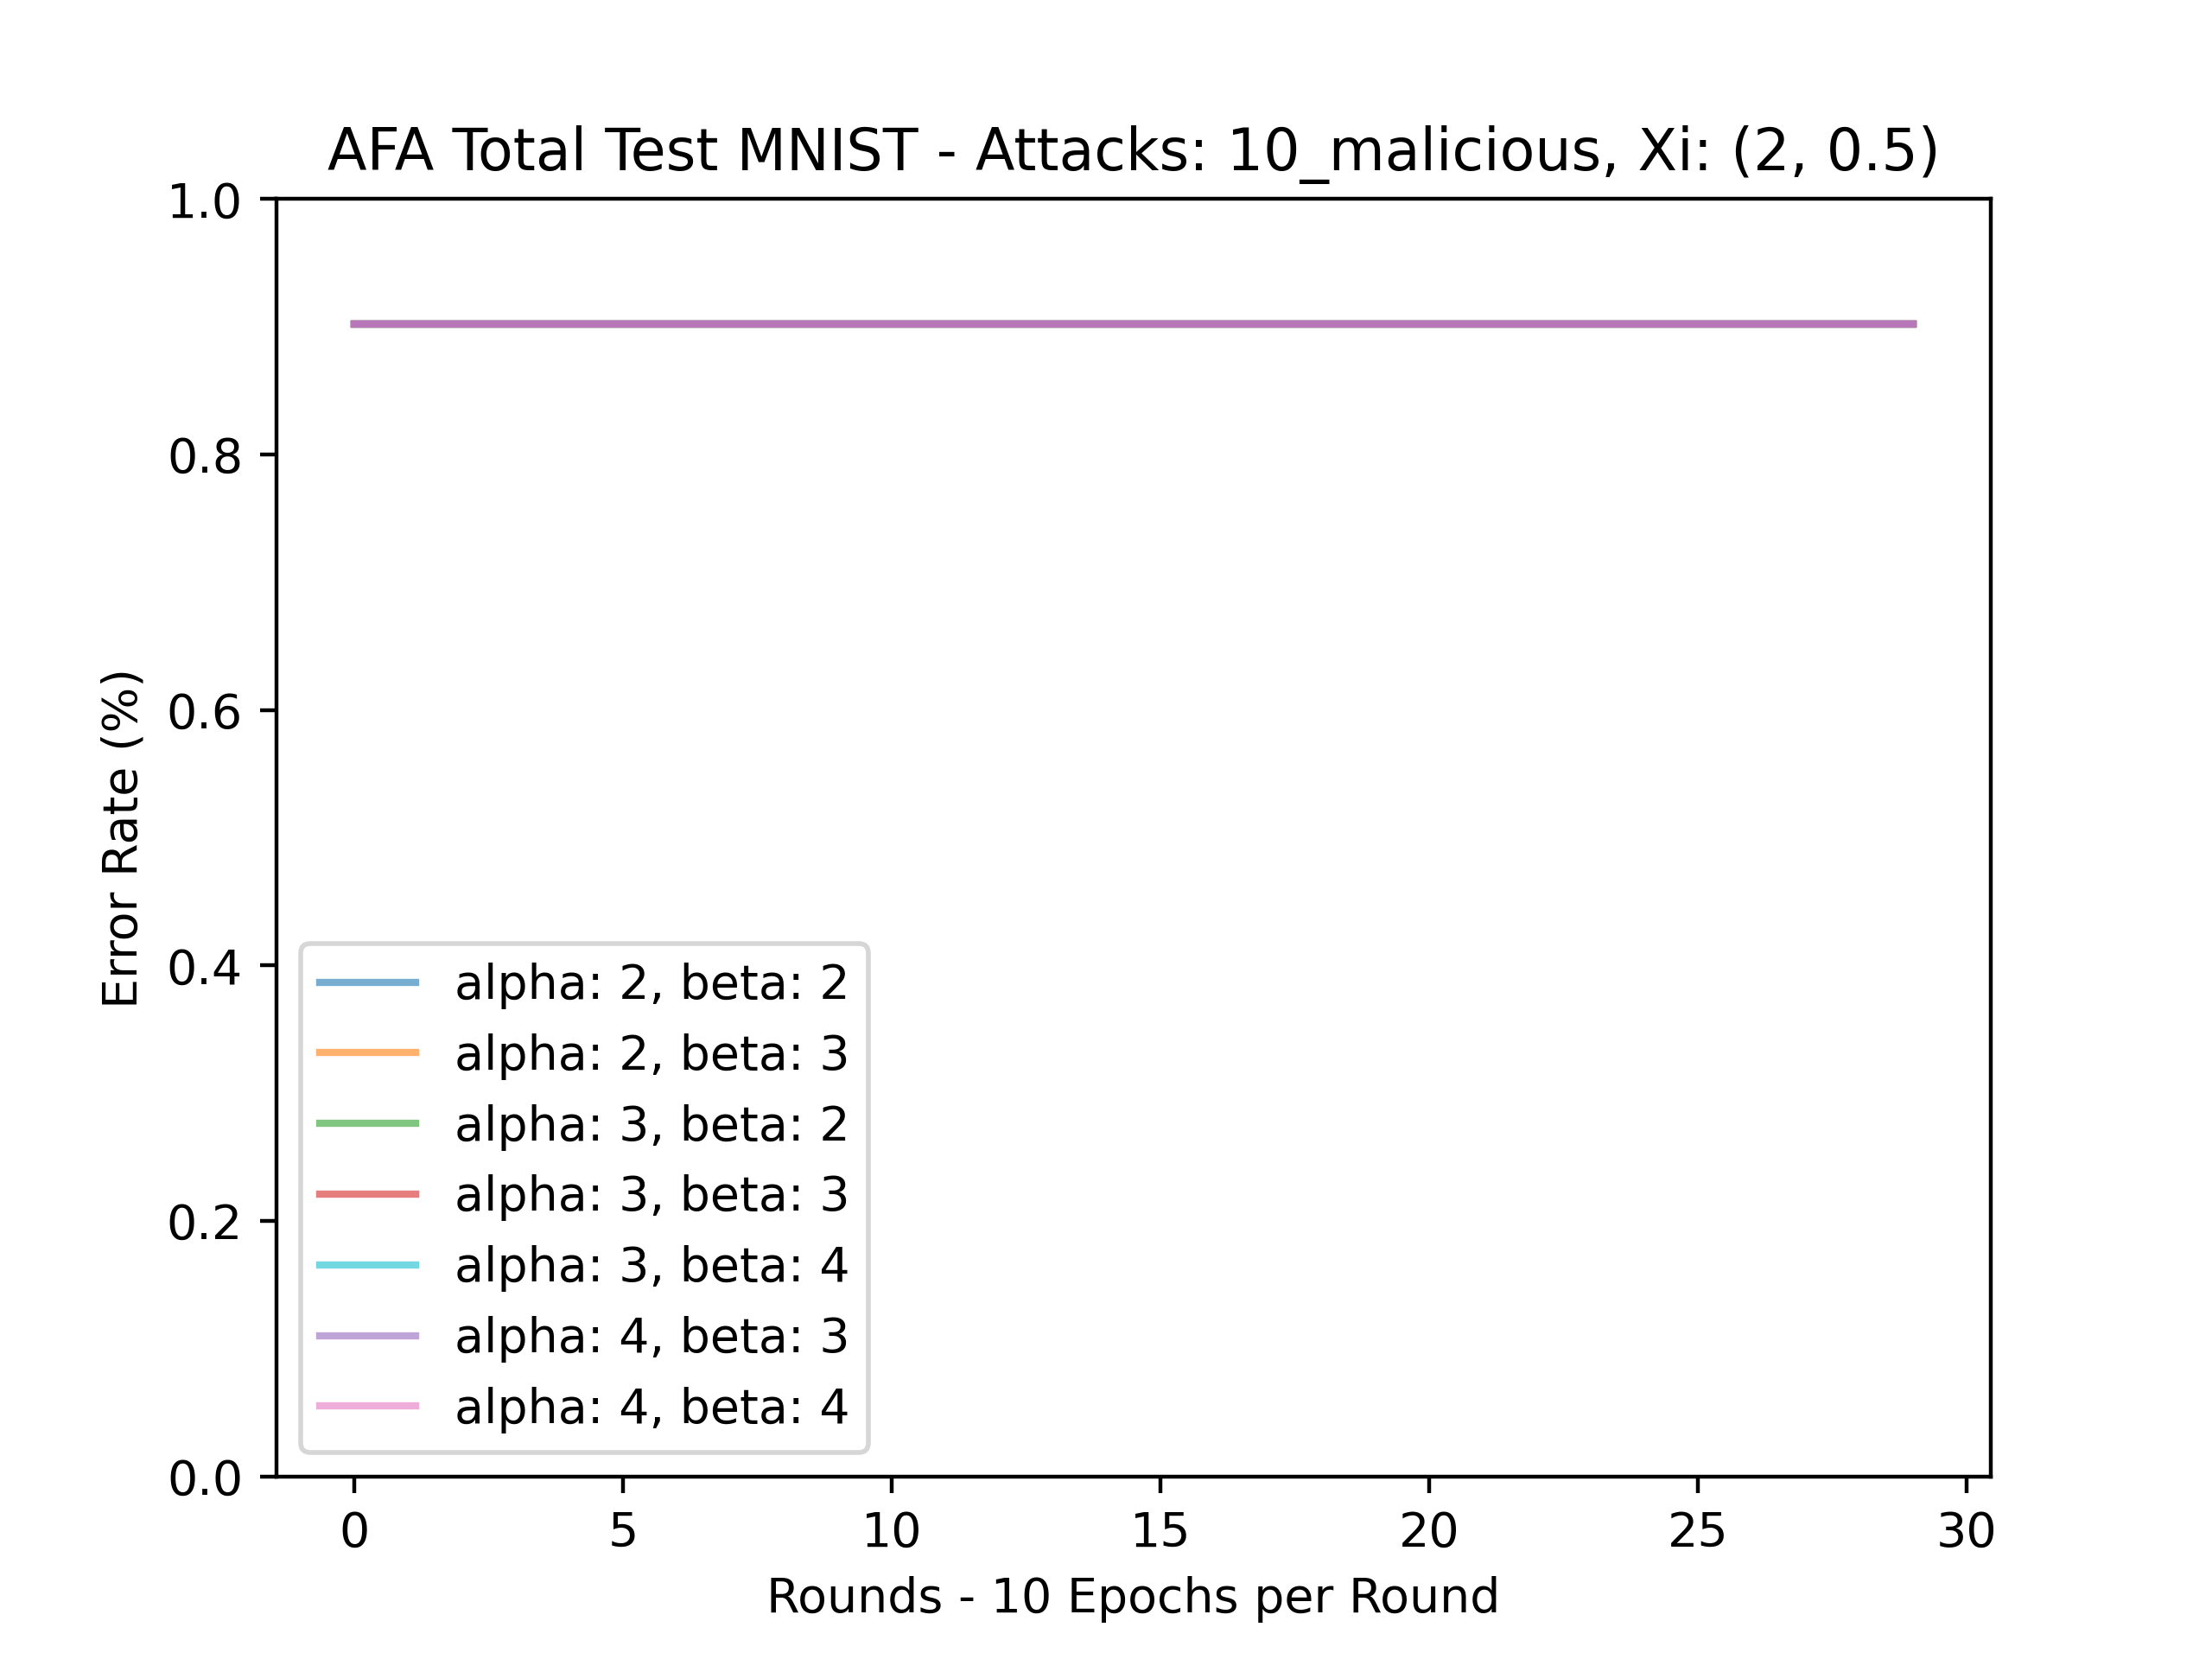
\includegraphics[scale=0.5]{initial/graphs/malicious_afa.png}
	\caption{10 Malicious clients in AFA}
	\label{fig:mal_afa}
\end{figure}

\begin{figure}[htbp]
	\centering
    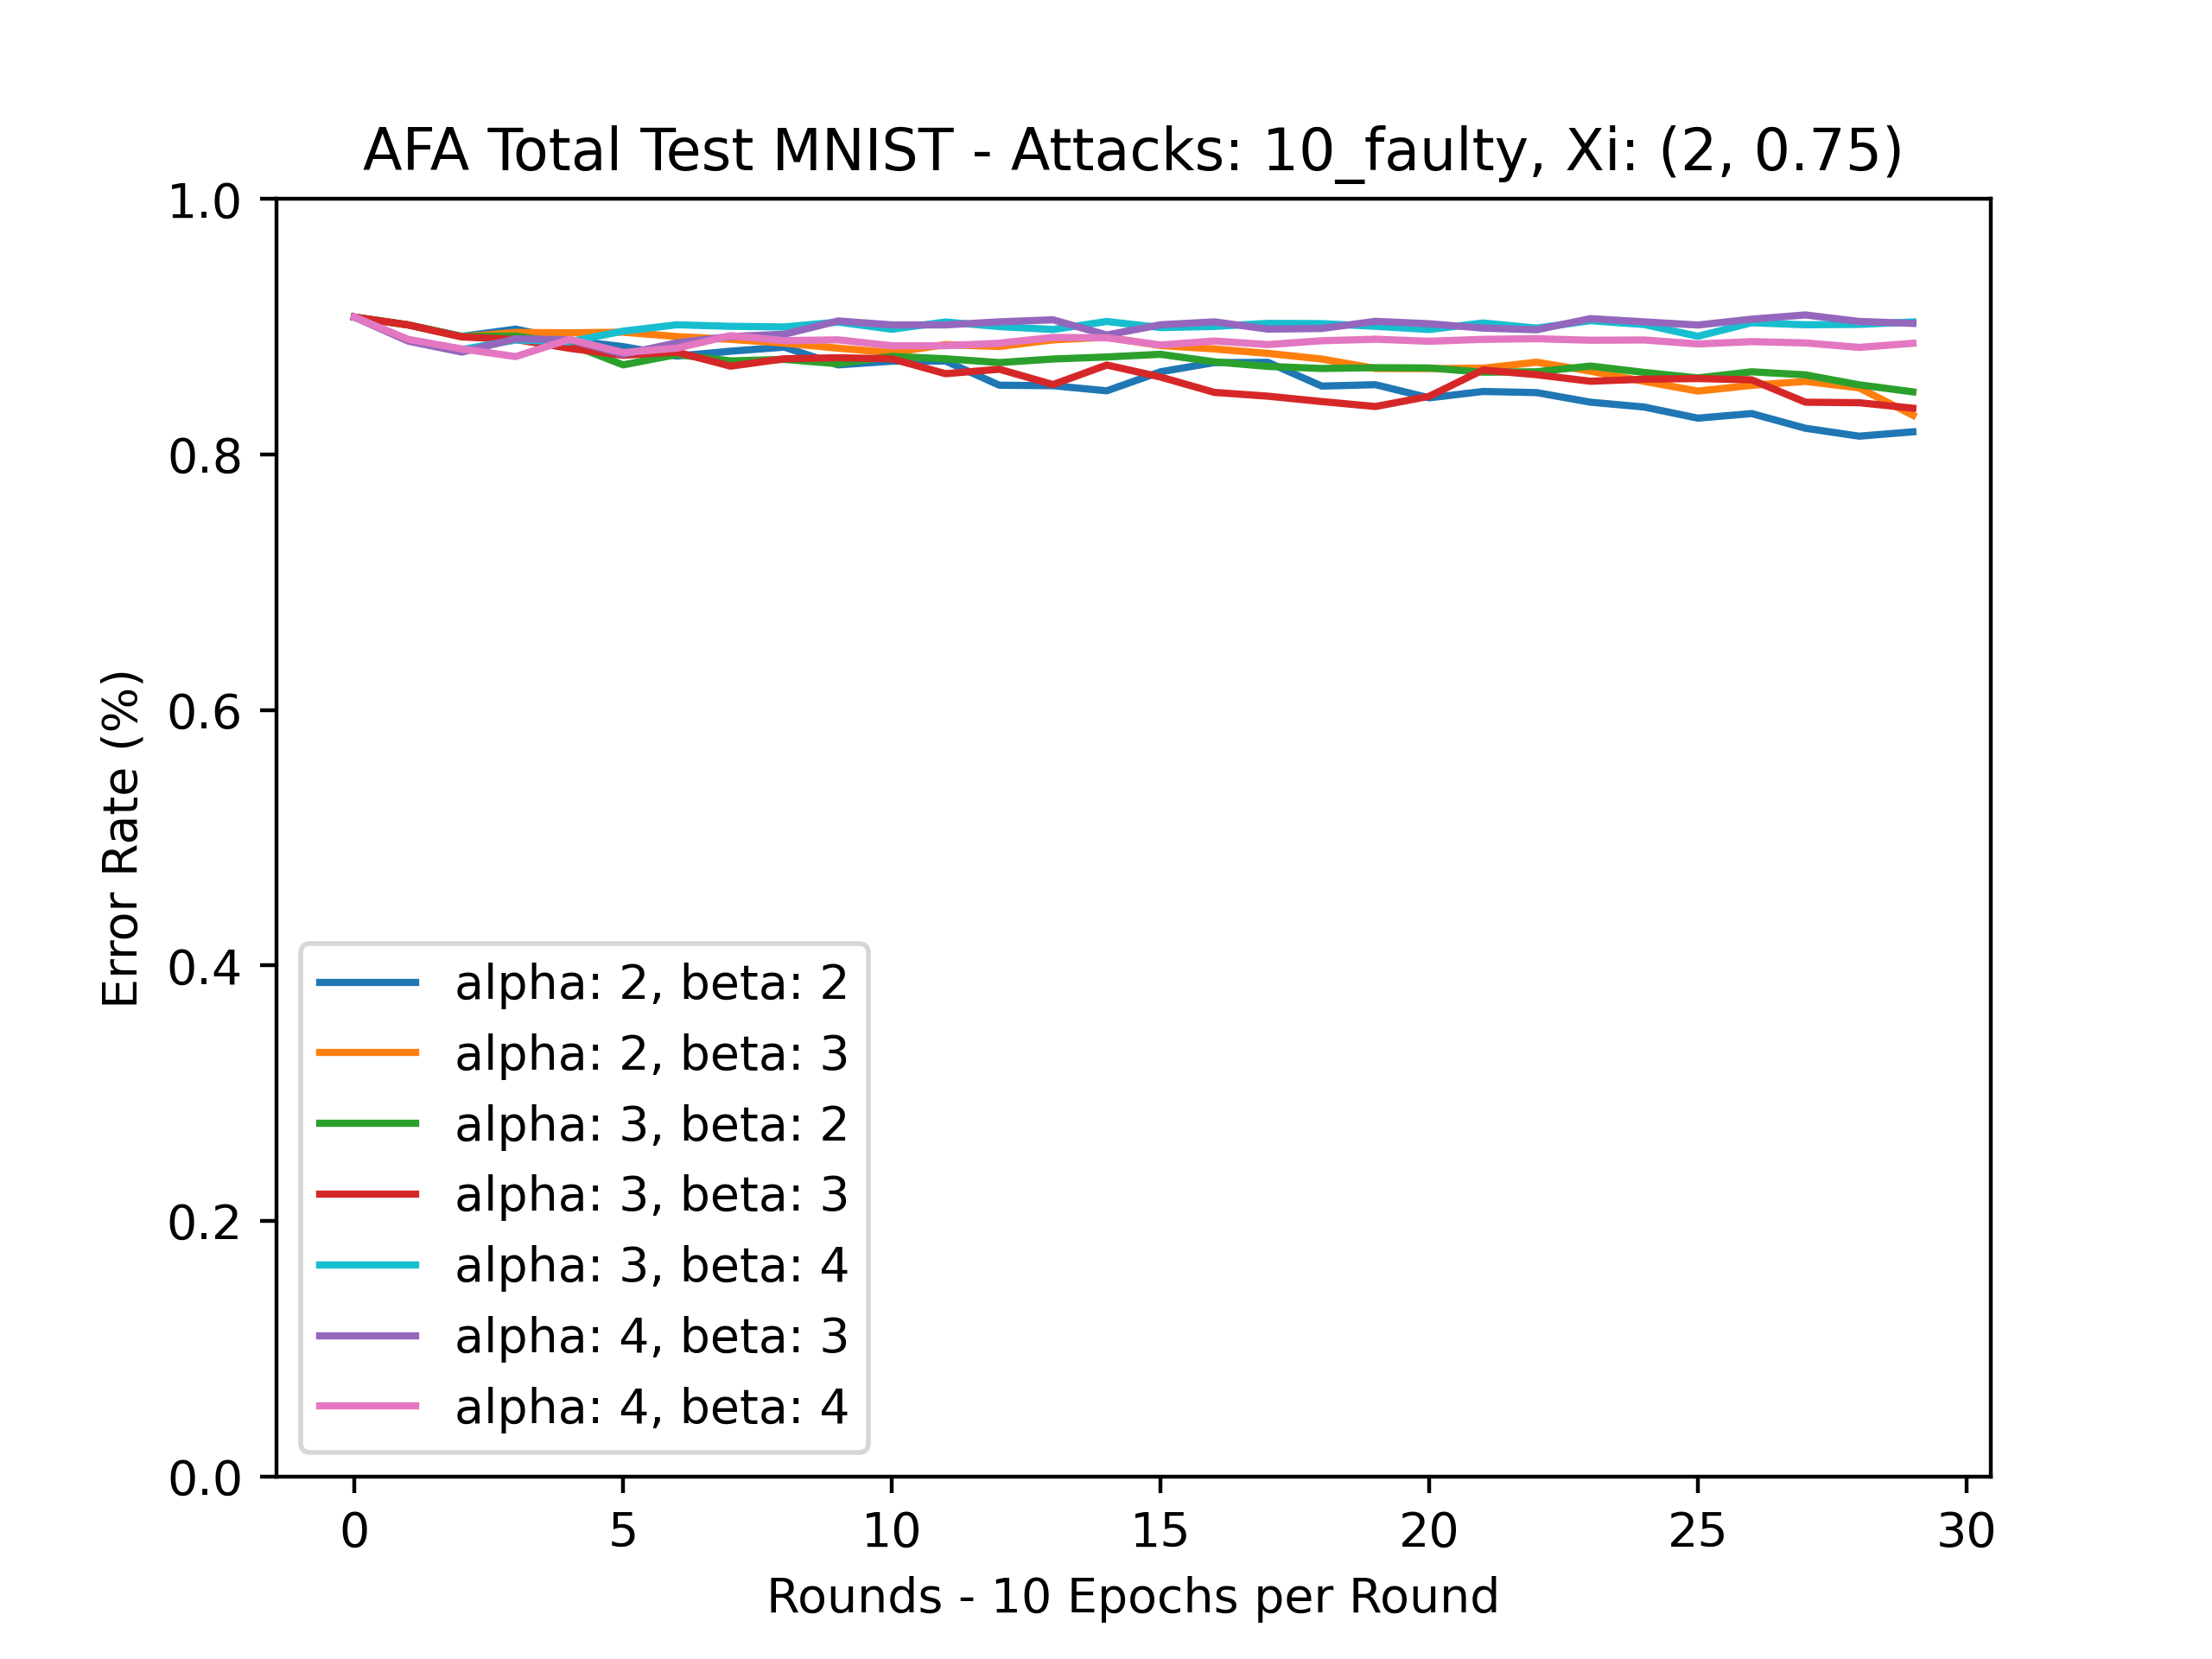
\includegraphics[scale=0.5]{initial/graphs/afa_2_0.75.png}
	\caption{AFA - Xi: 2, DeltaXi: 0.75}
	\label{fig:afa_2_0.75}
\end{figure}

\begin{figure}[htbp]
	\centering
    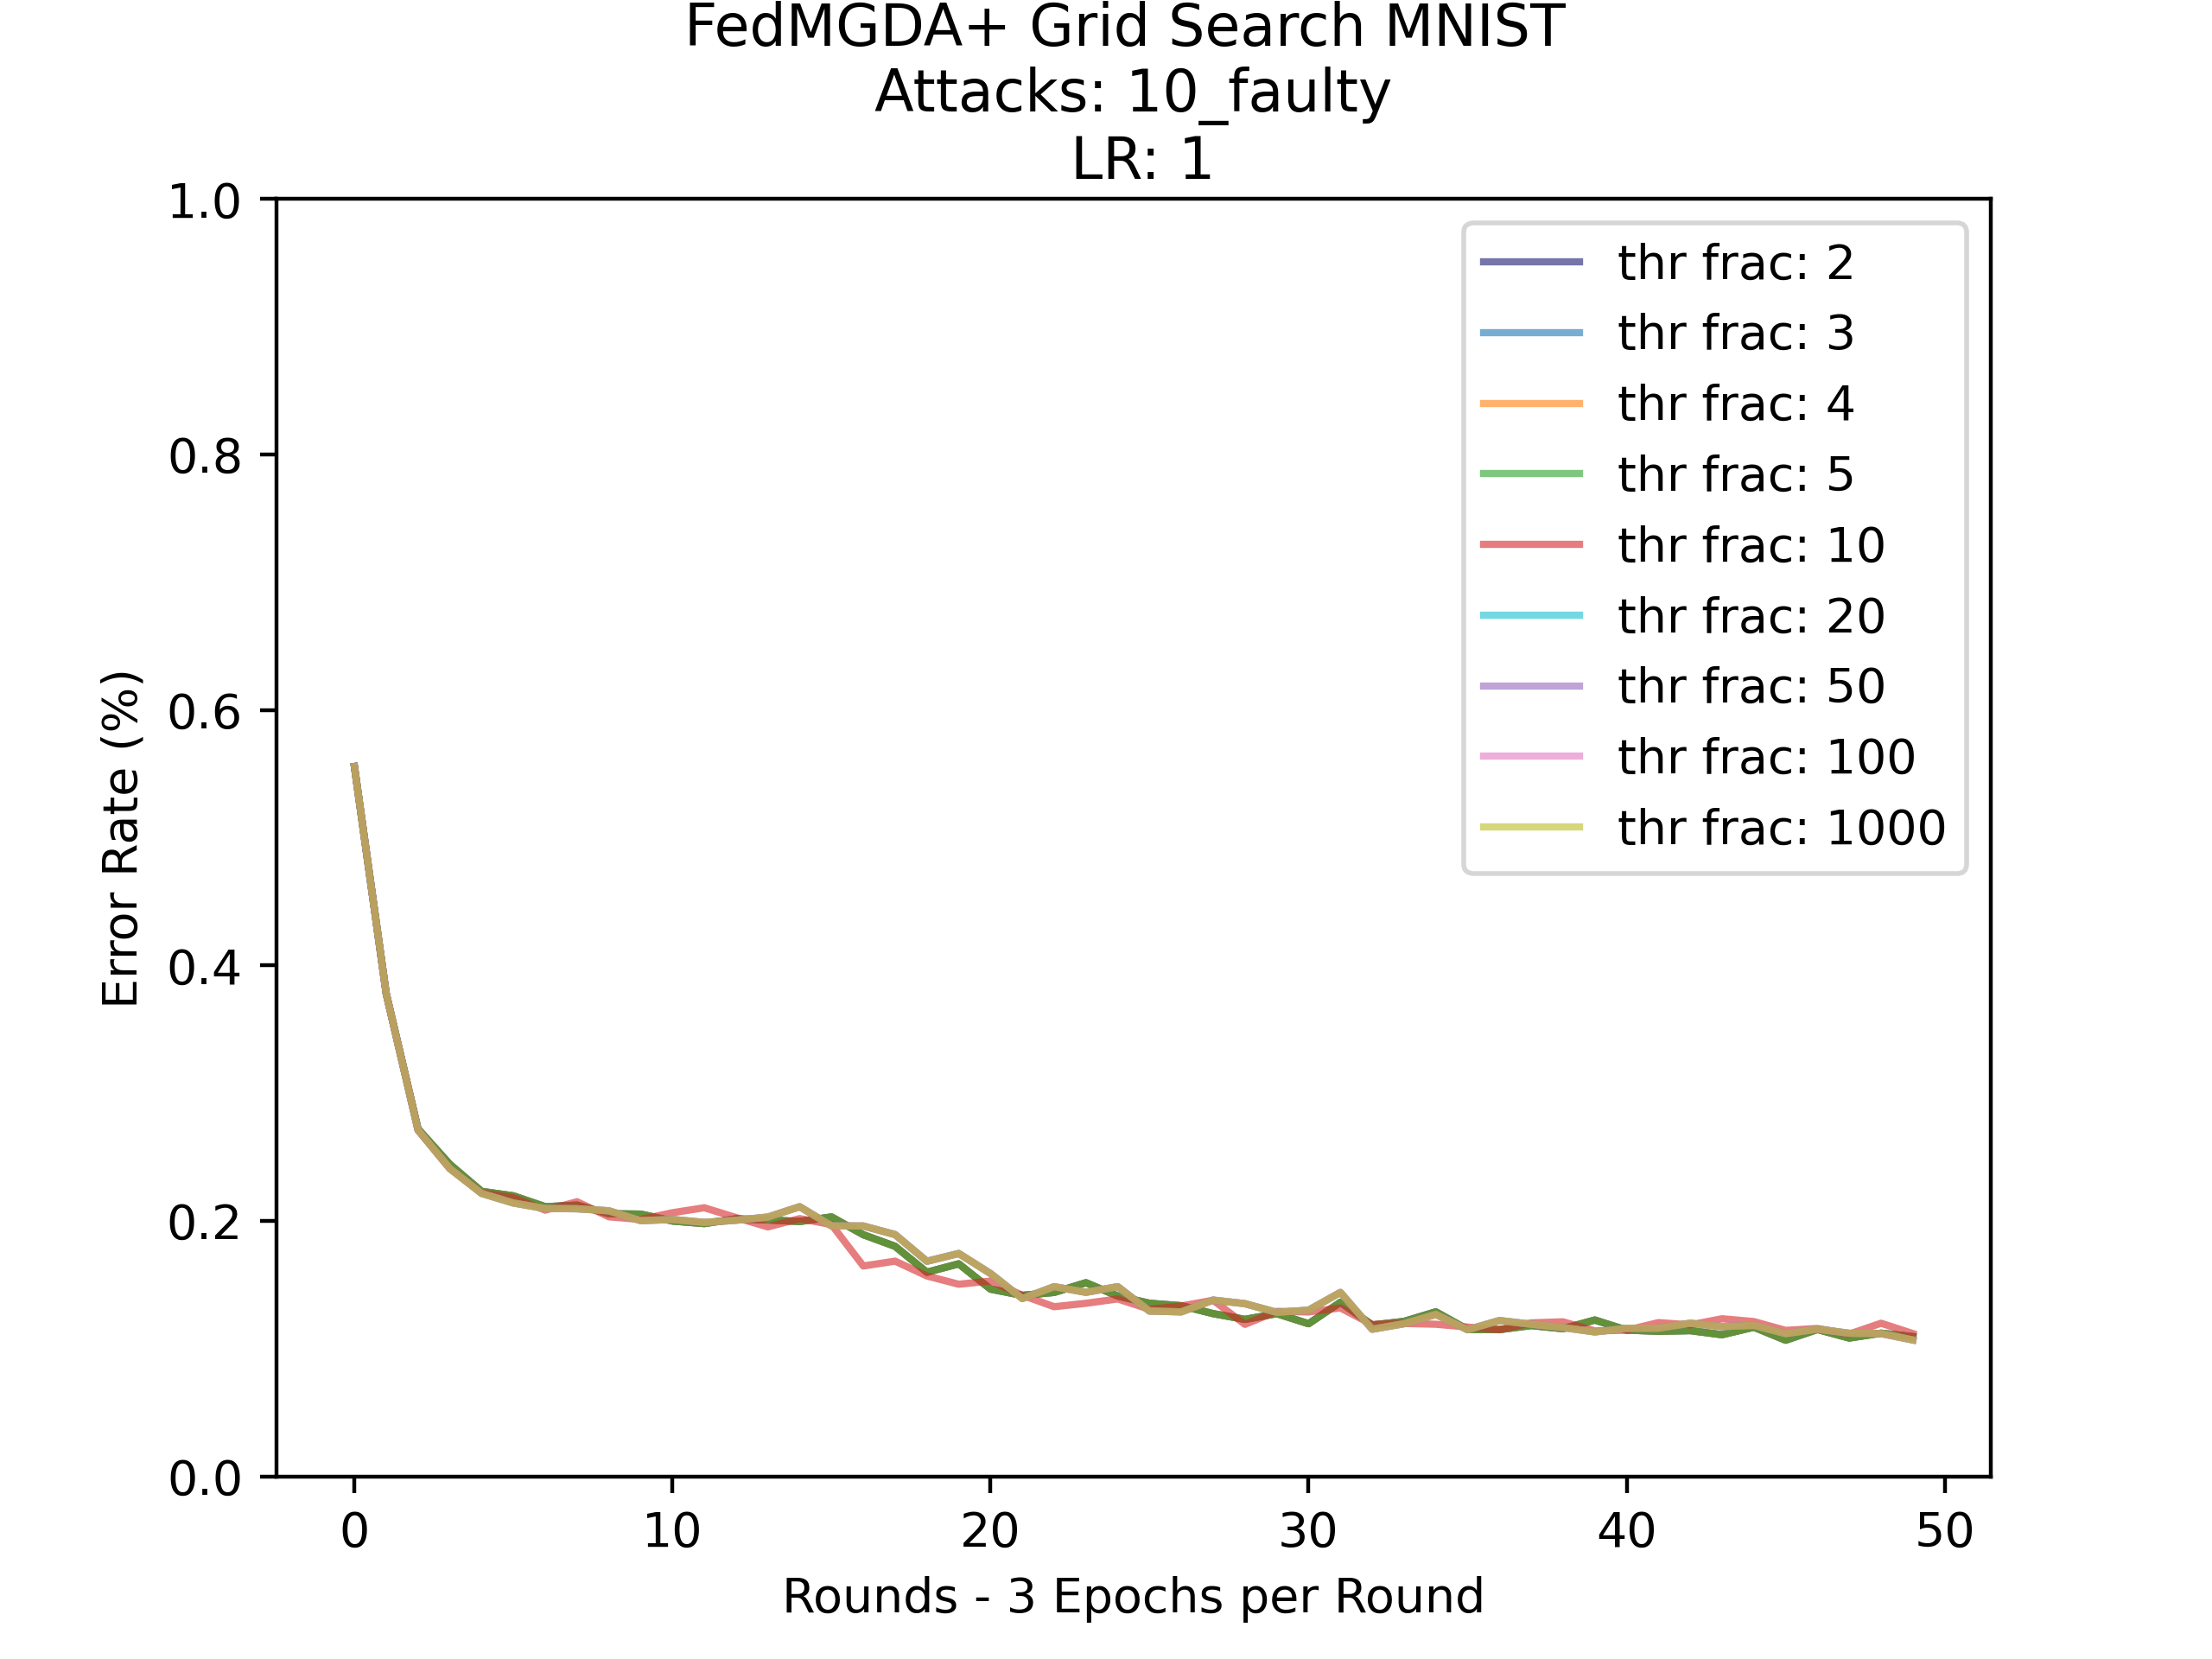
\includegraphics[scale=0.5]{initial/graphs/mgda_var.png}
	\caption{FedMGDA+ Threshold Variance Demo}
	\label{fig:mgda_var}
\end{figure}

\begin{figure}[htbp]
	\centering
    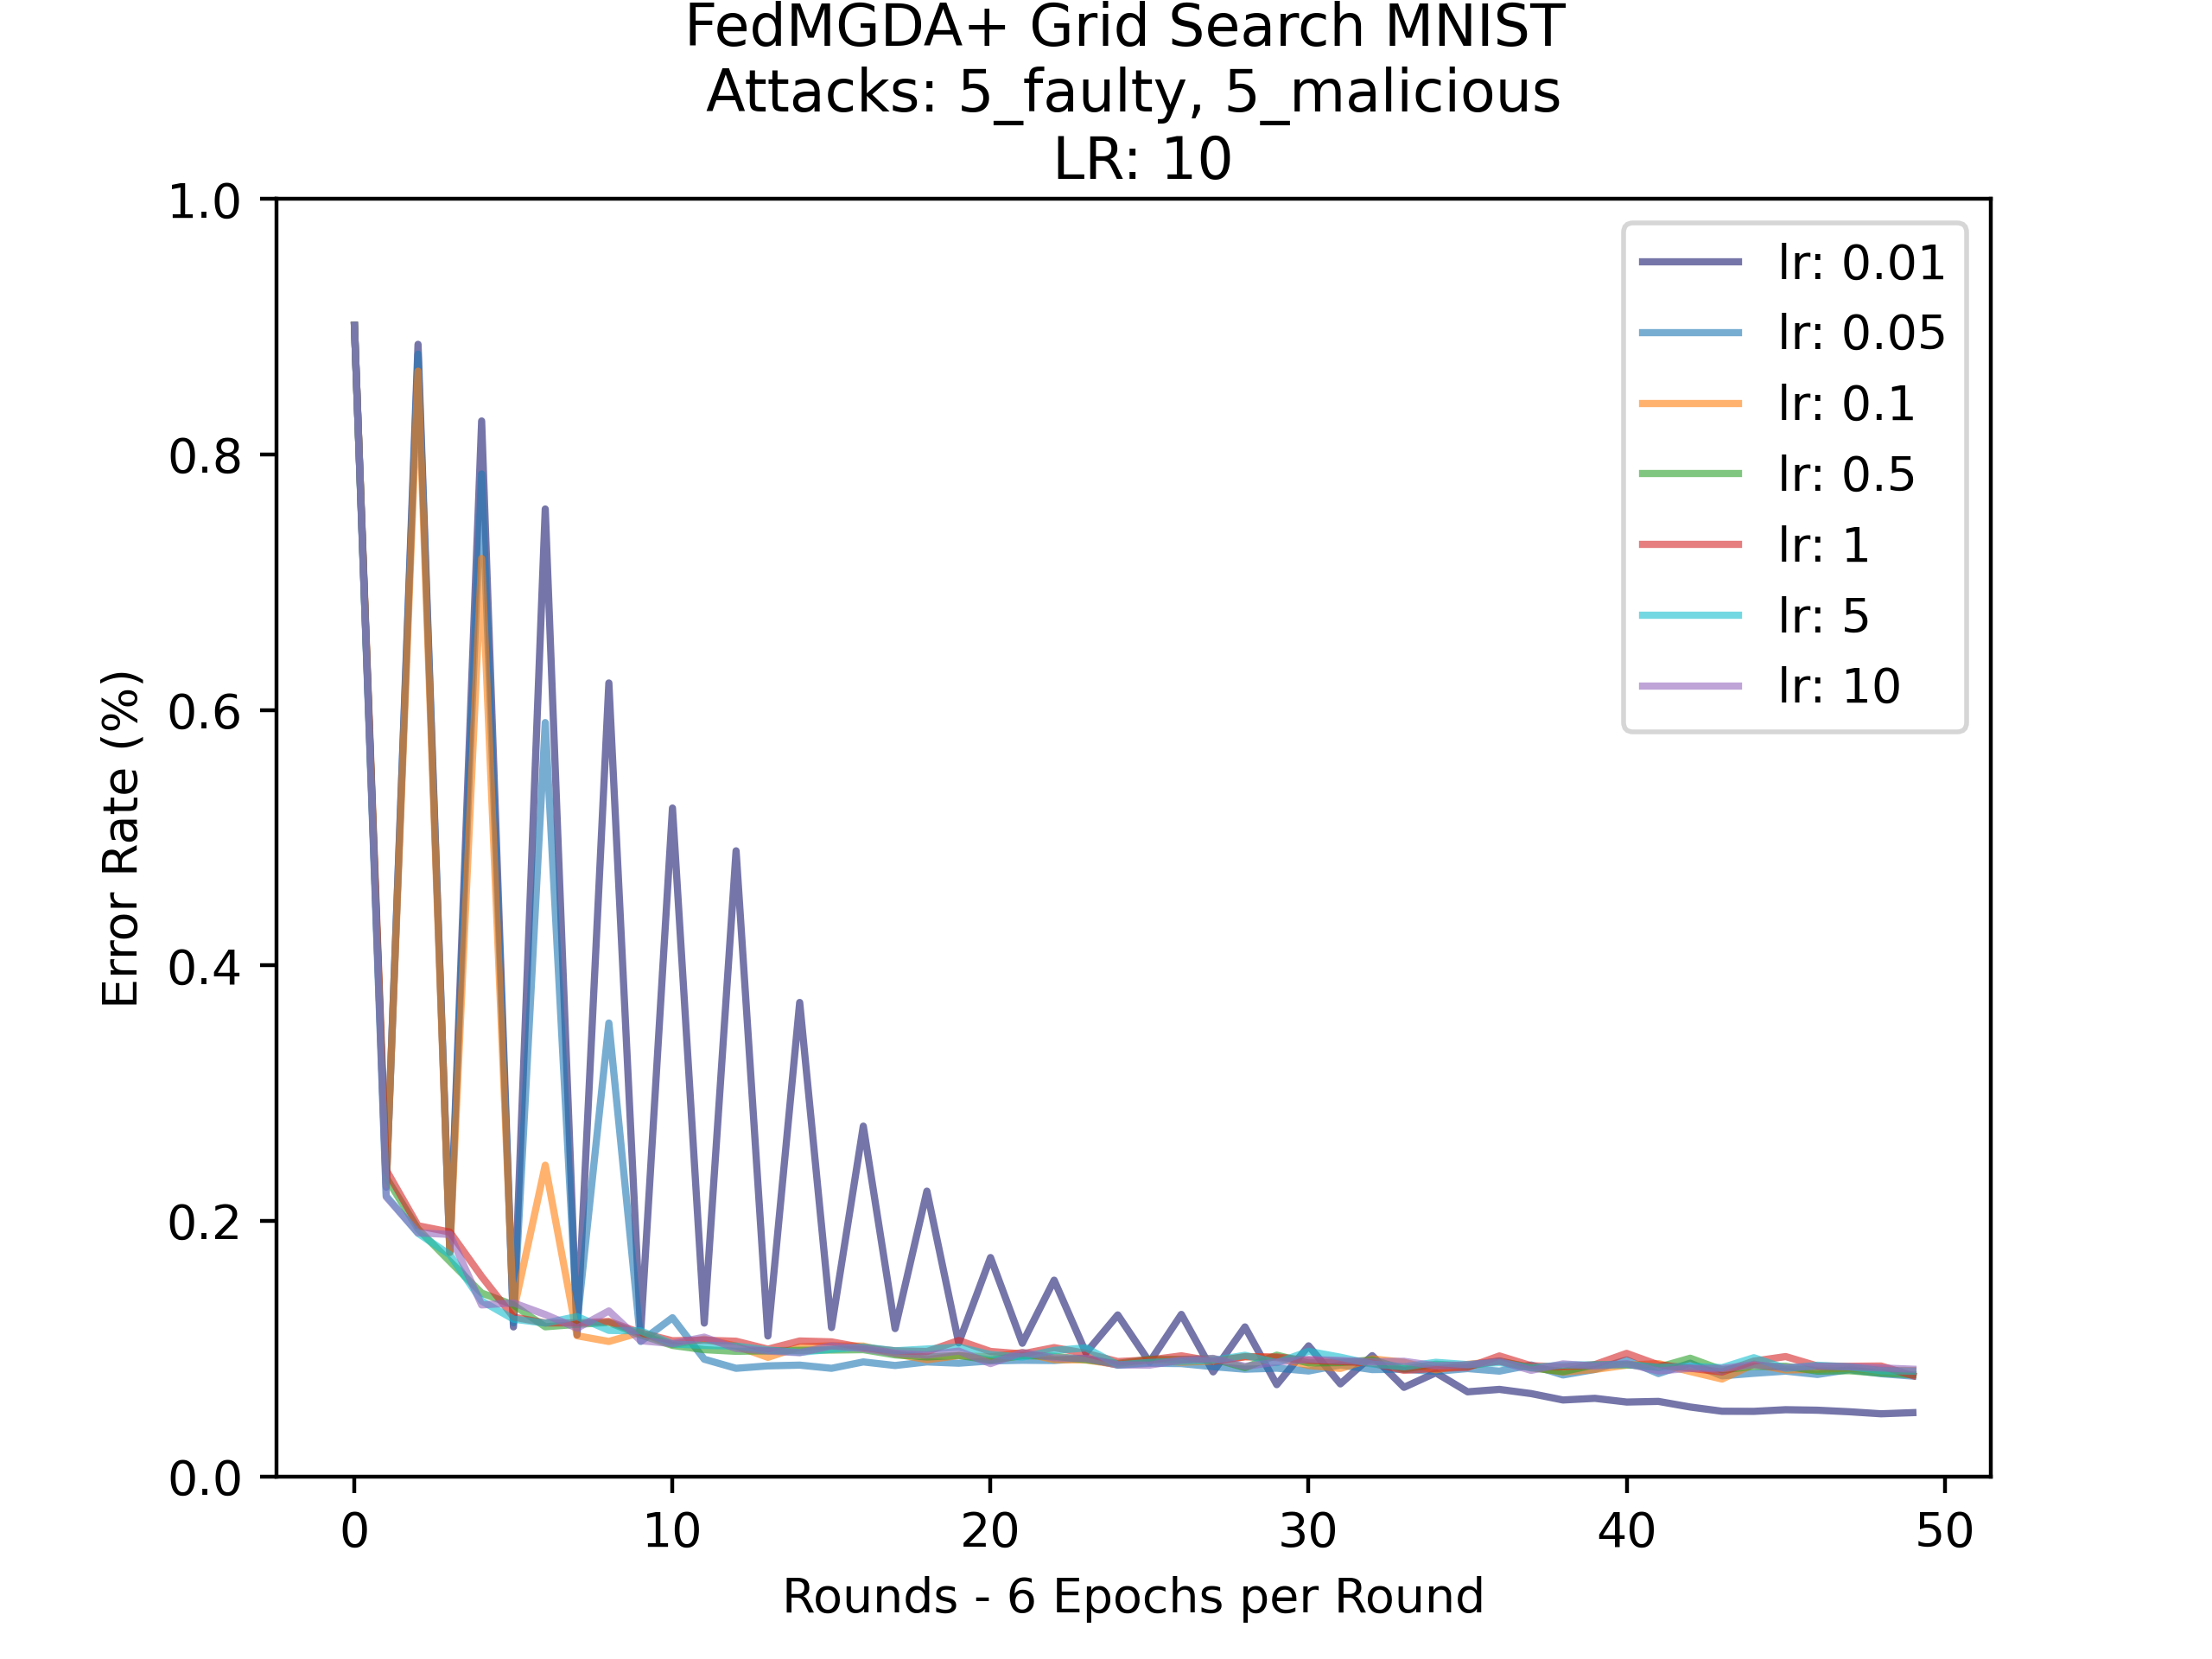
\includegraphics[scale=0.5]{initial/graphs/fake_good.png}
	\caption{FedMGDA+ Quick Convergence}
	\label{fig:fake_good}
\end{figure}

\begin{figure}[htbp]
	\centering
    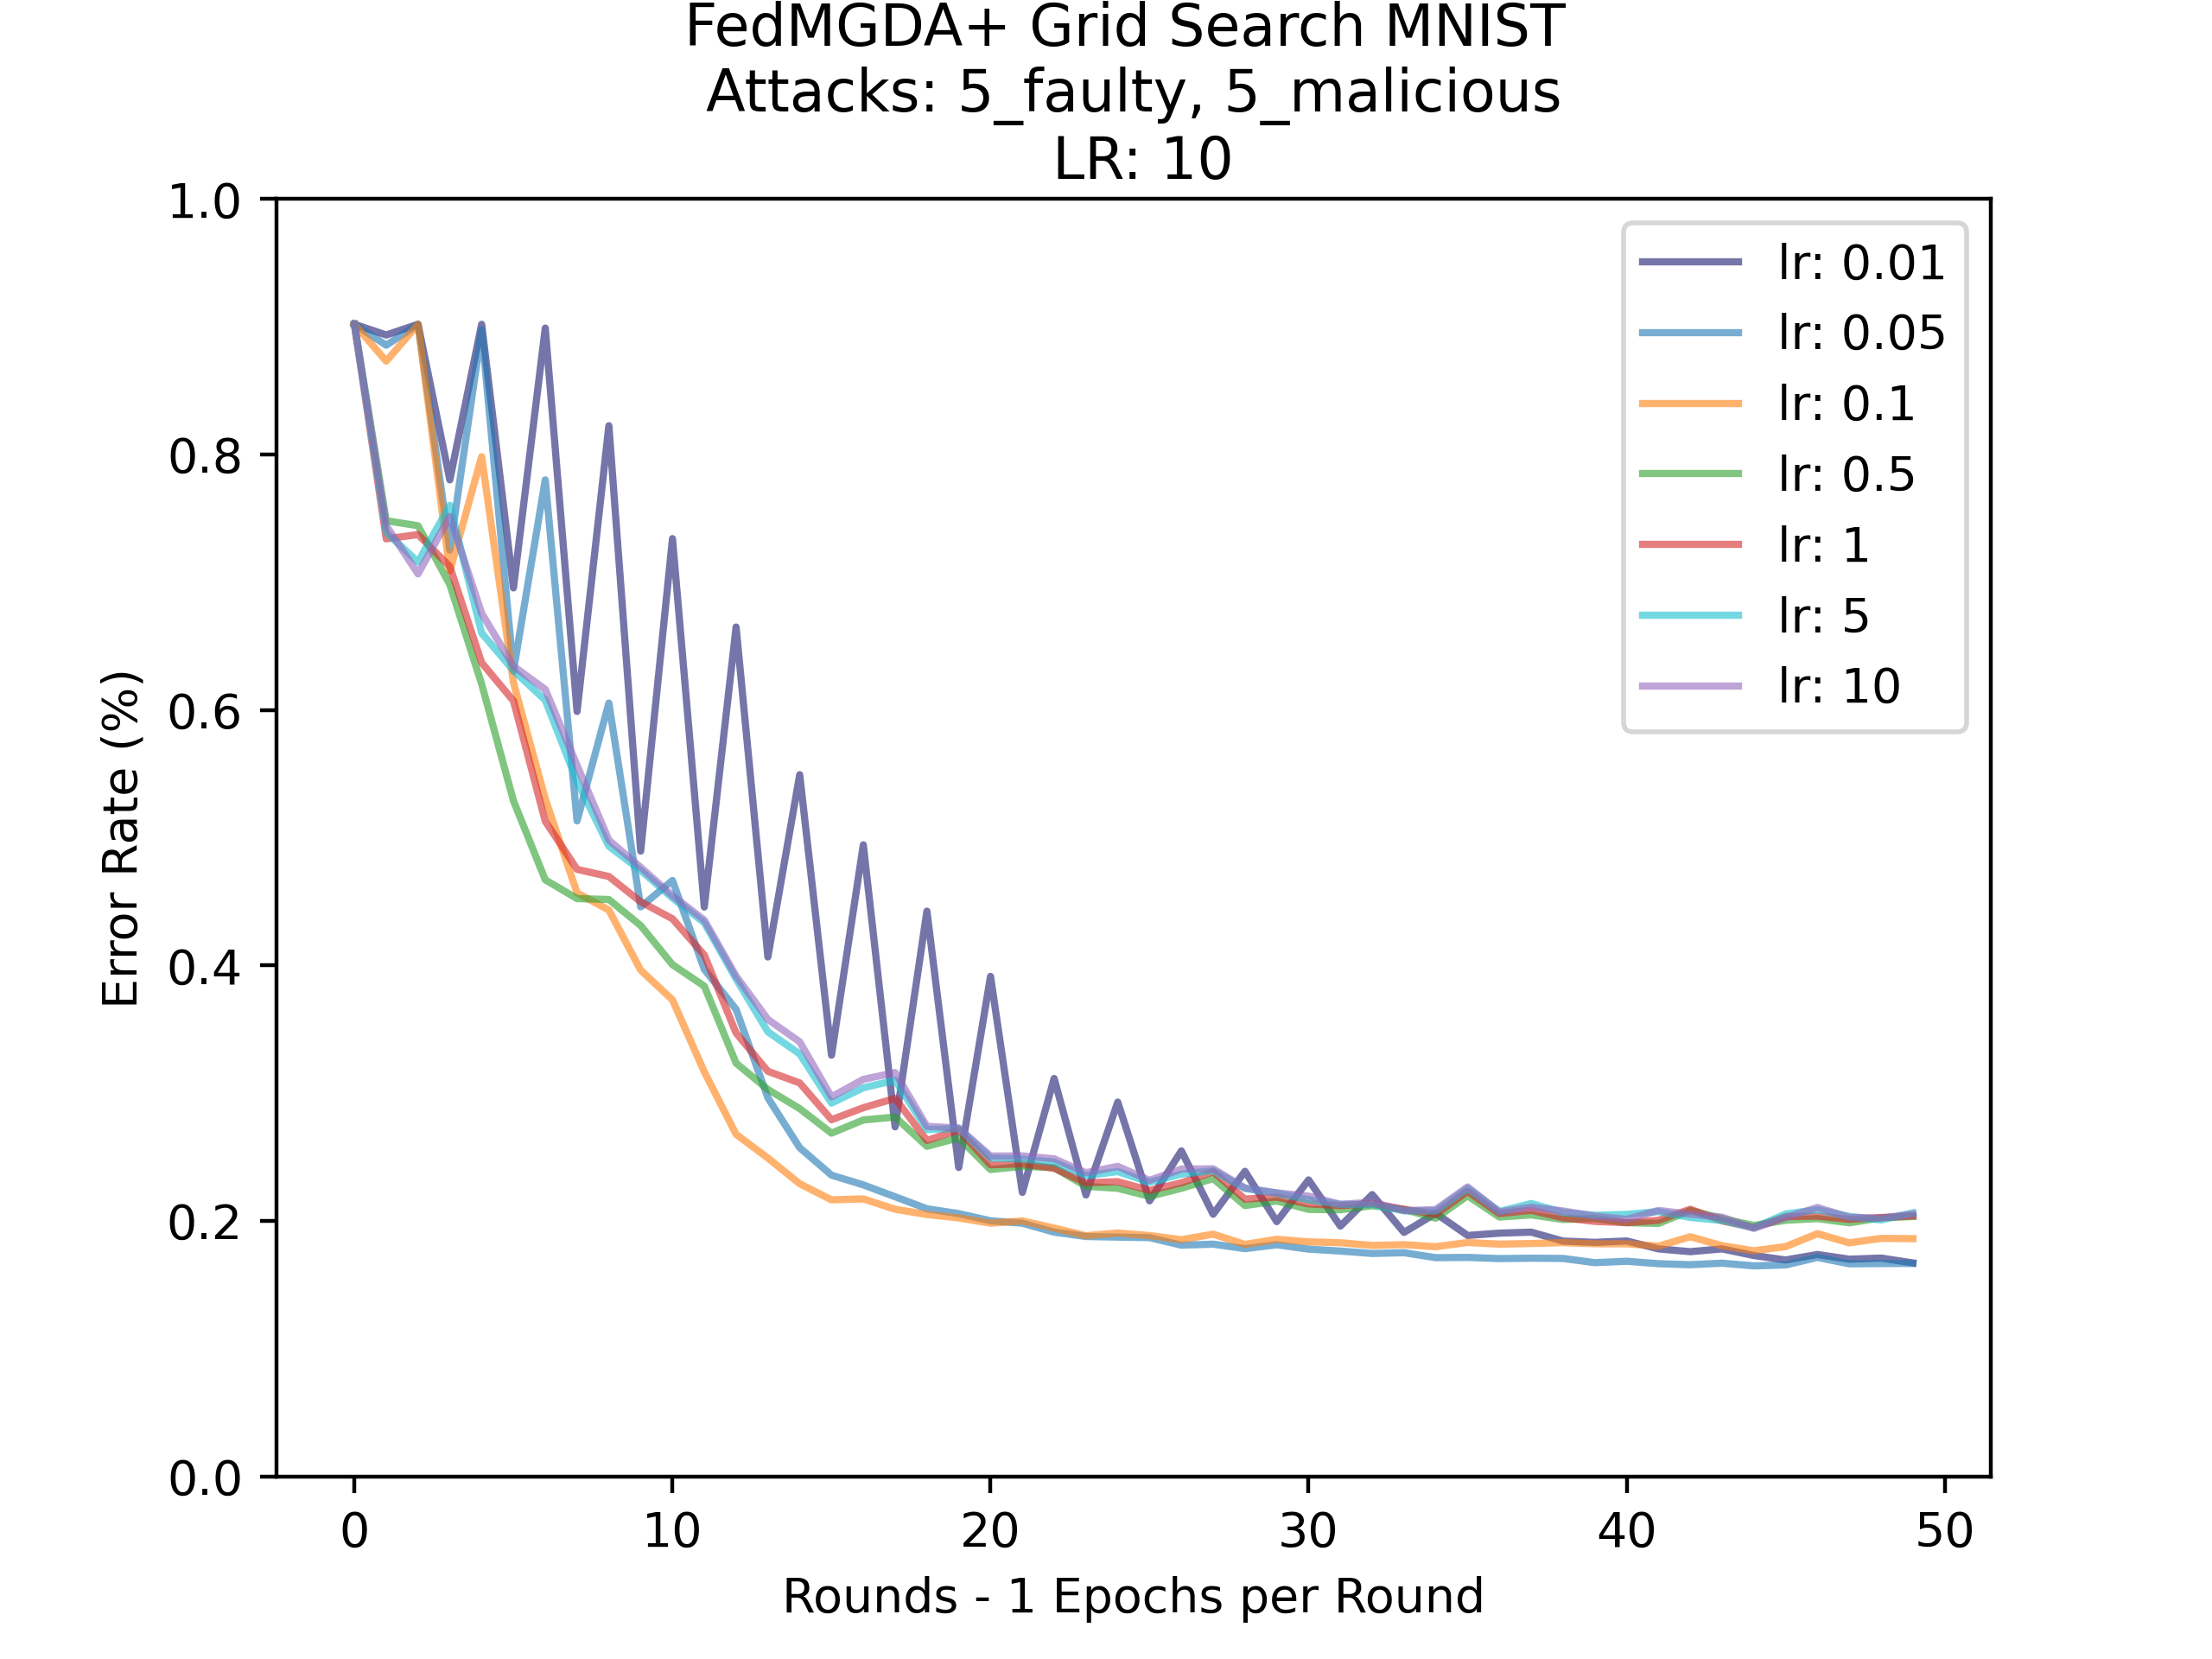
\includegraphics[scale=0.5]{initial/graphs/1epoch_grid.png}
	\caption{FedMGDA+ with No Benign Blocked but High Error Rate}
	\label{fig:1epoch_grid}
\end{figure}

\begin{figure}[htbp]
	\centering
    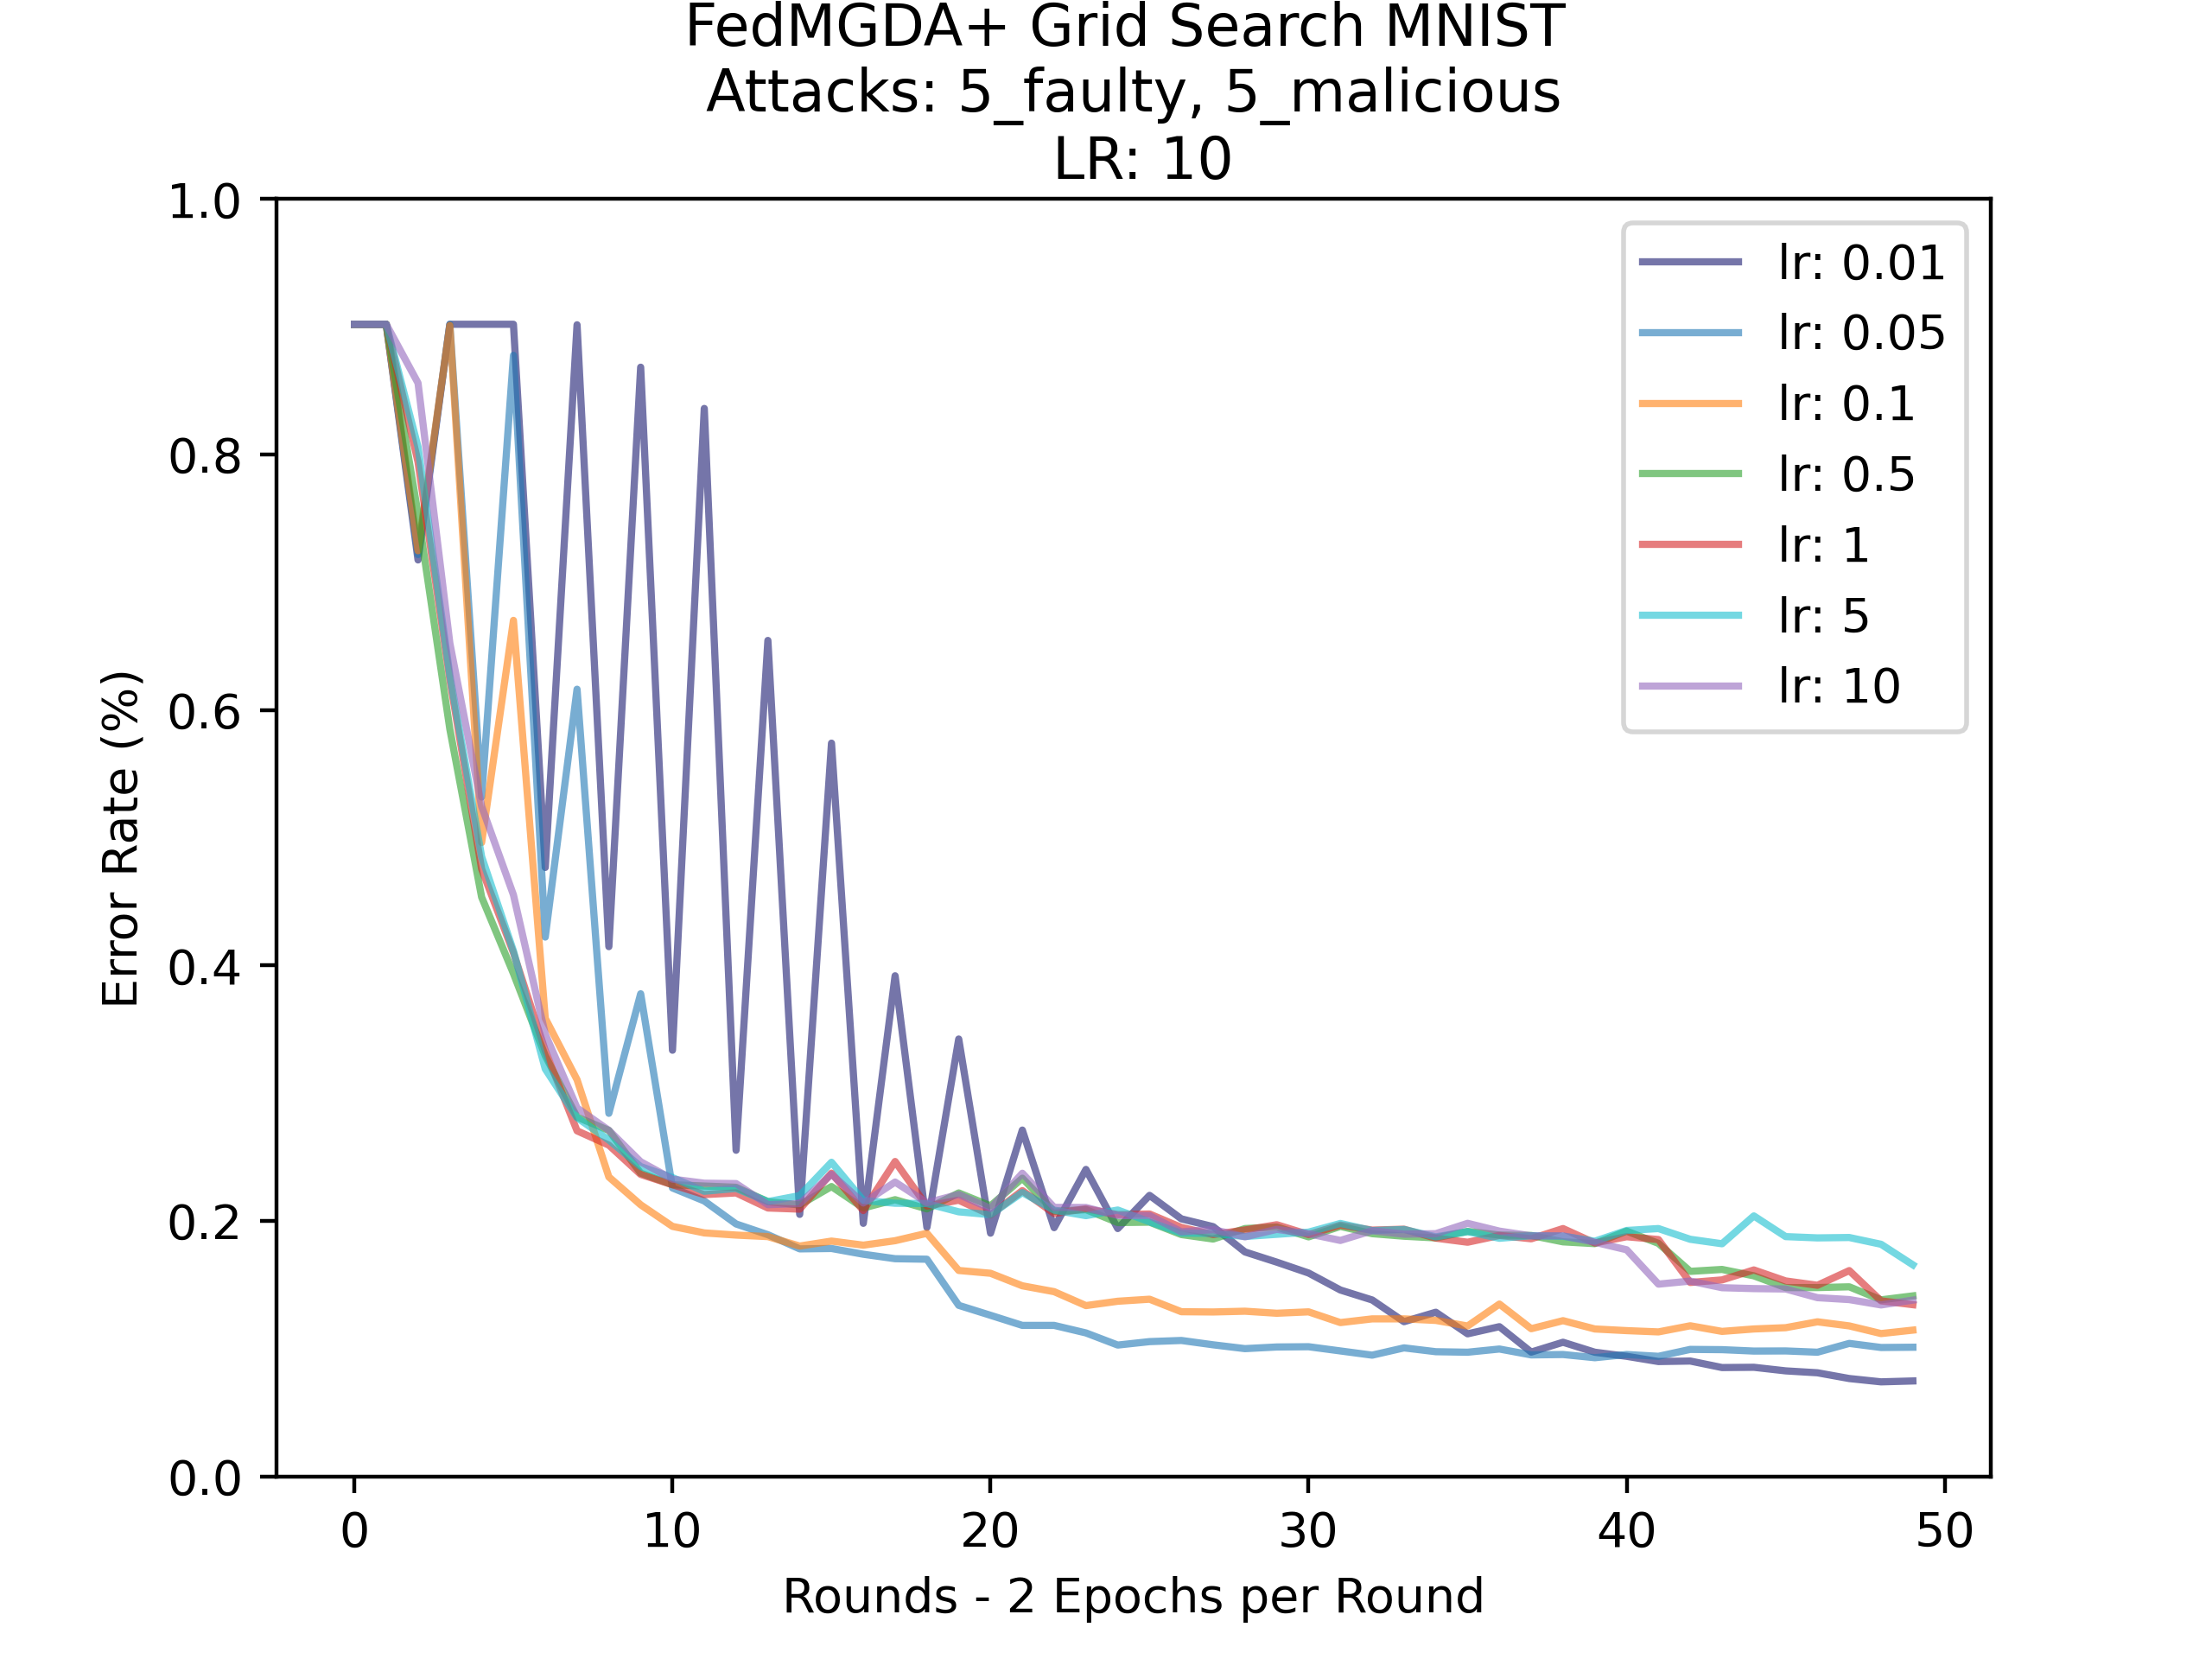
\includegraphics[scale=0.5]{initial/graphs/2epoch_grid.png}
	\caption{FedMGDA+ Benign Blocked Late but Low Error Rate}
	\label{fig:2epoch_grid}
\end{figure}

\begin{figure}[htbp]
	\centering
    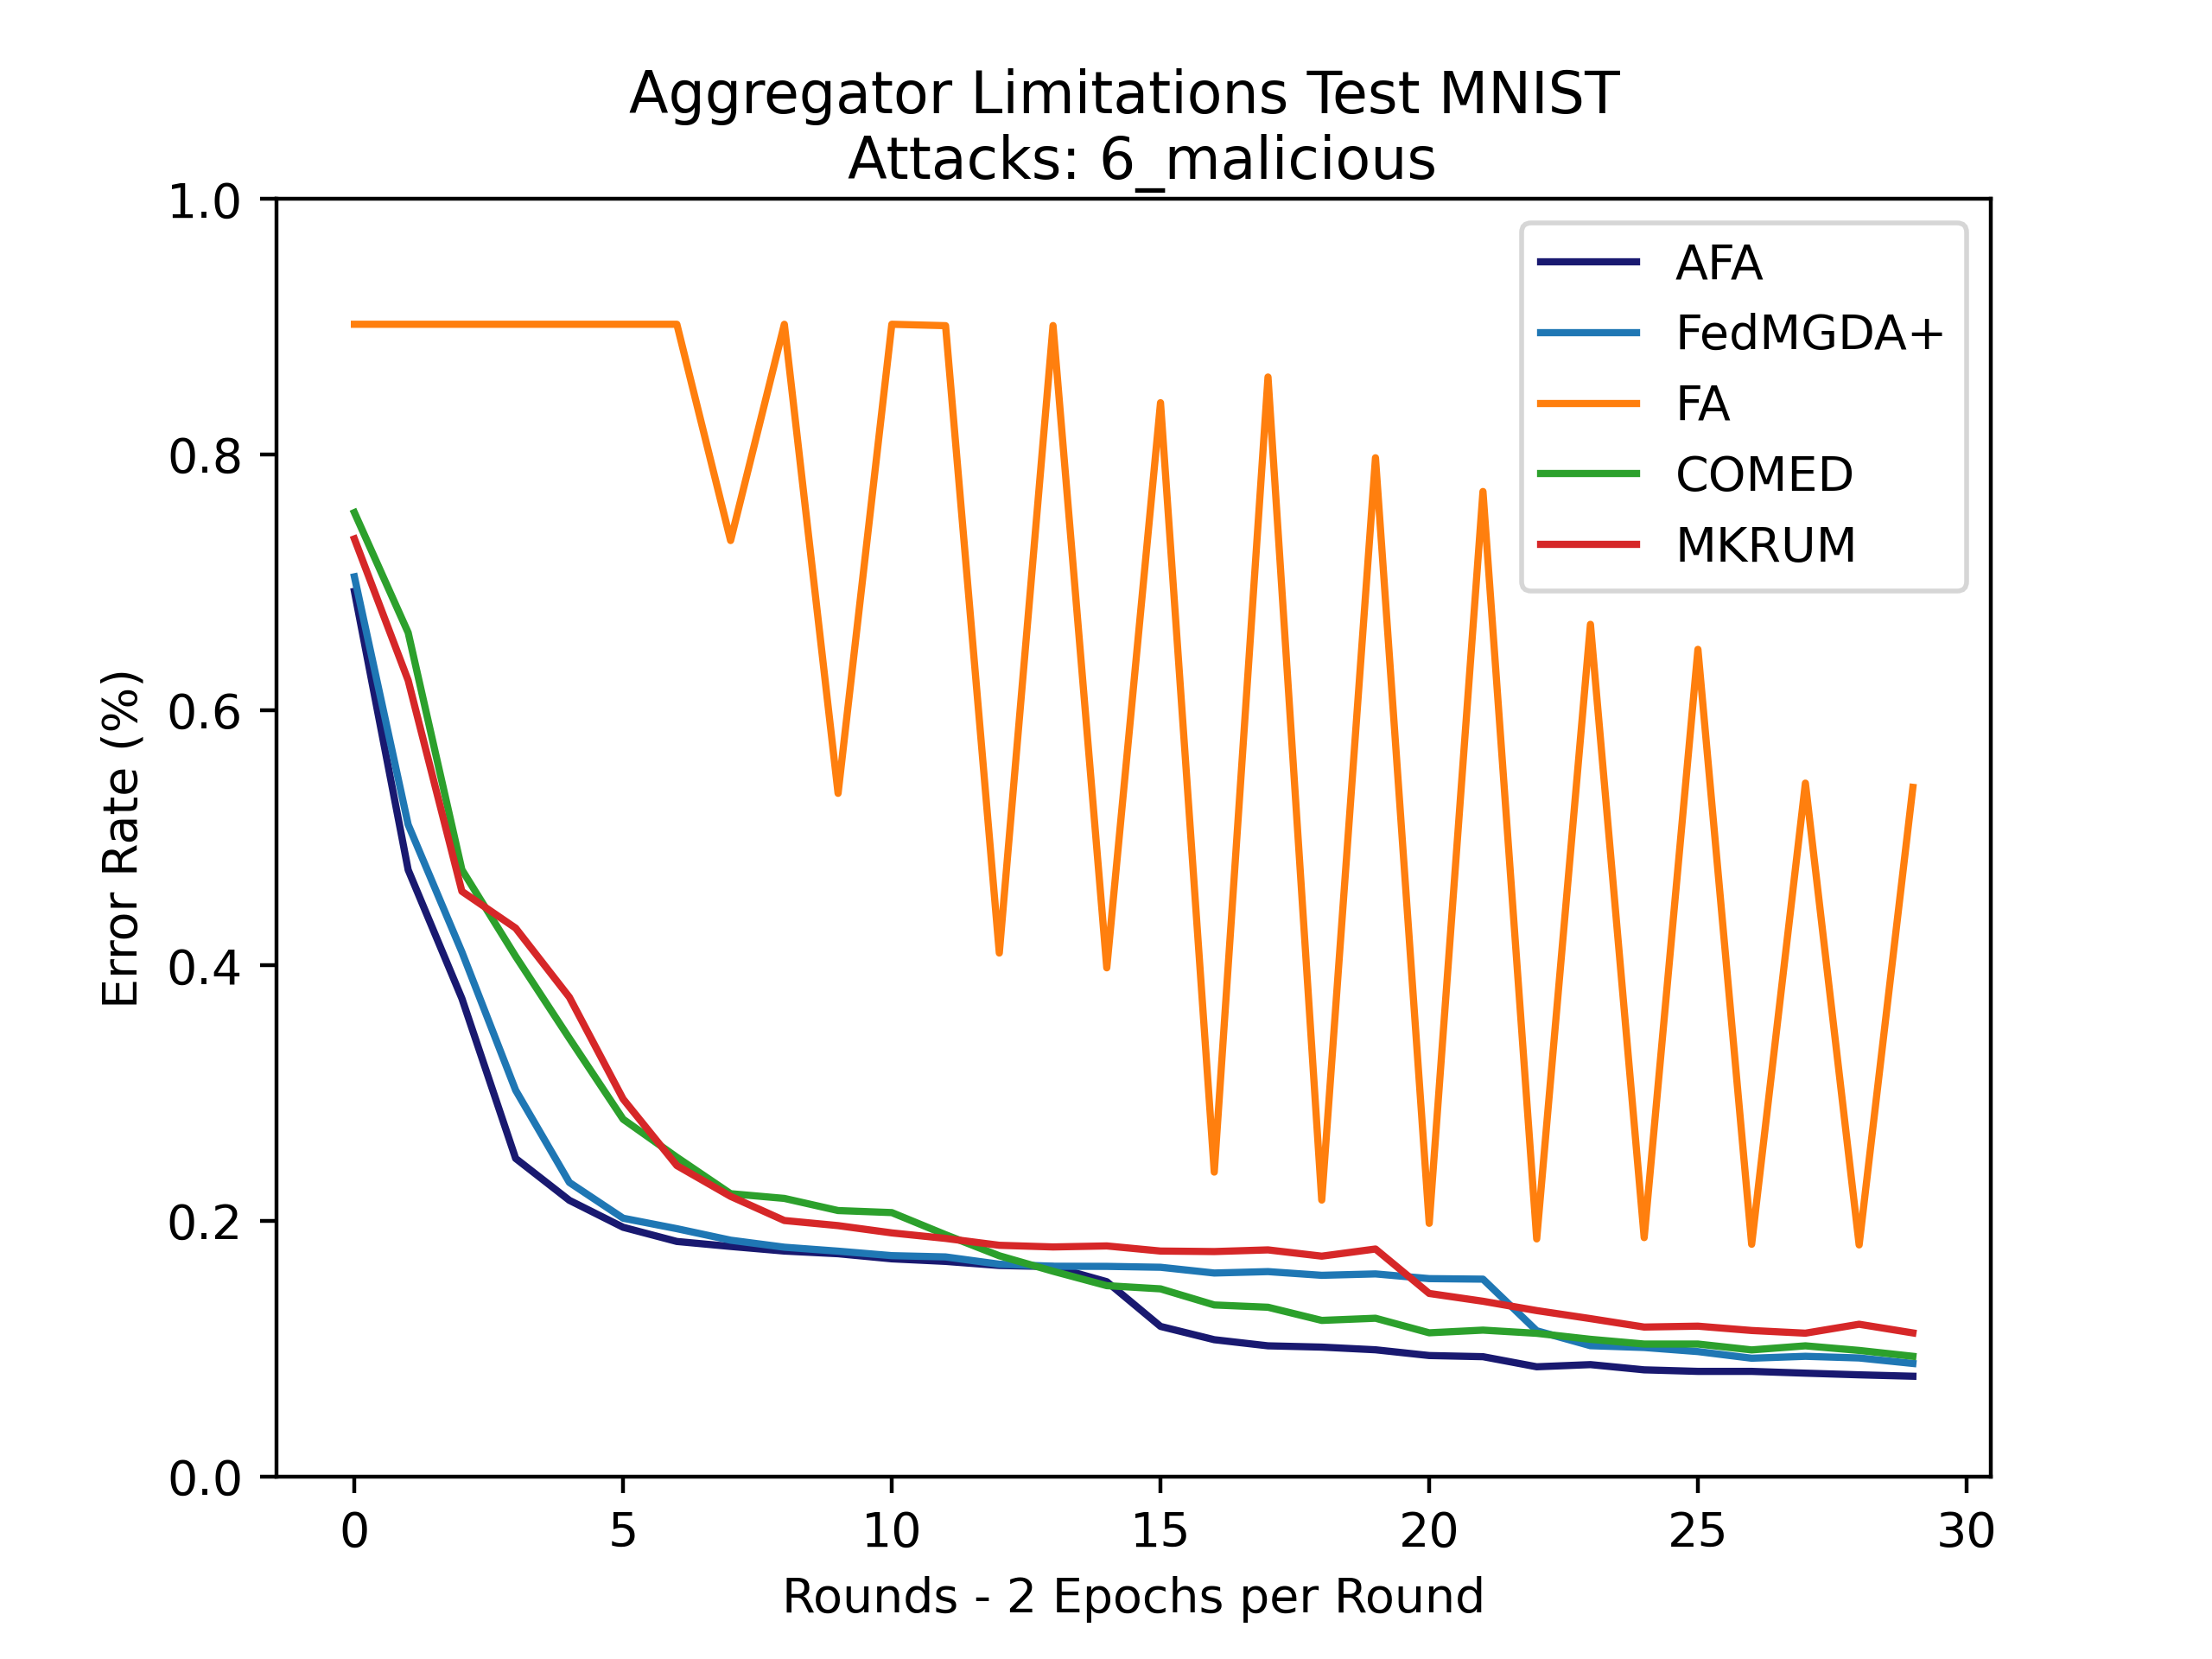
\includegraphics[scale=0.5]{initial/graphs/6_malicious.png}
	\caption{FedAvg Failing to Converge with Noticeable Damage in the Training Process}
	\label{fig:6mal}
\end{figure}

\begin{figure}[htbp]
	\centering
    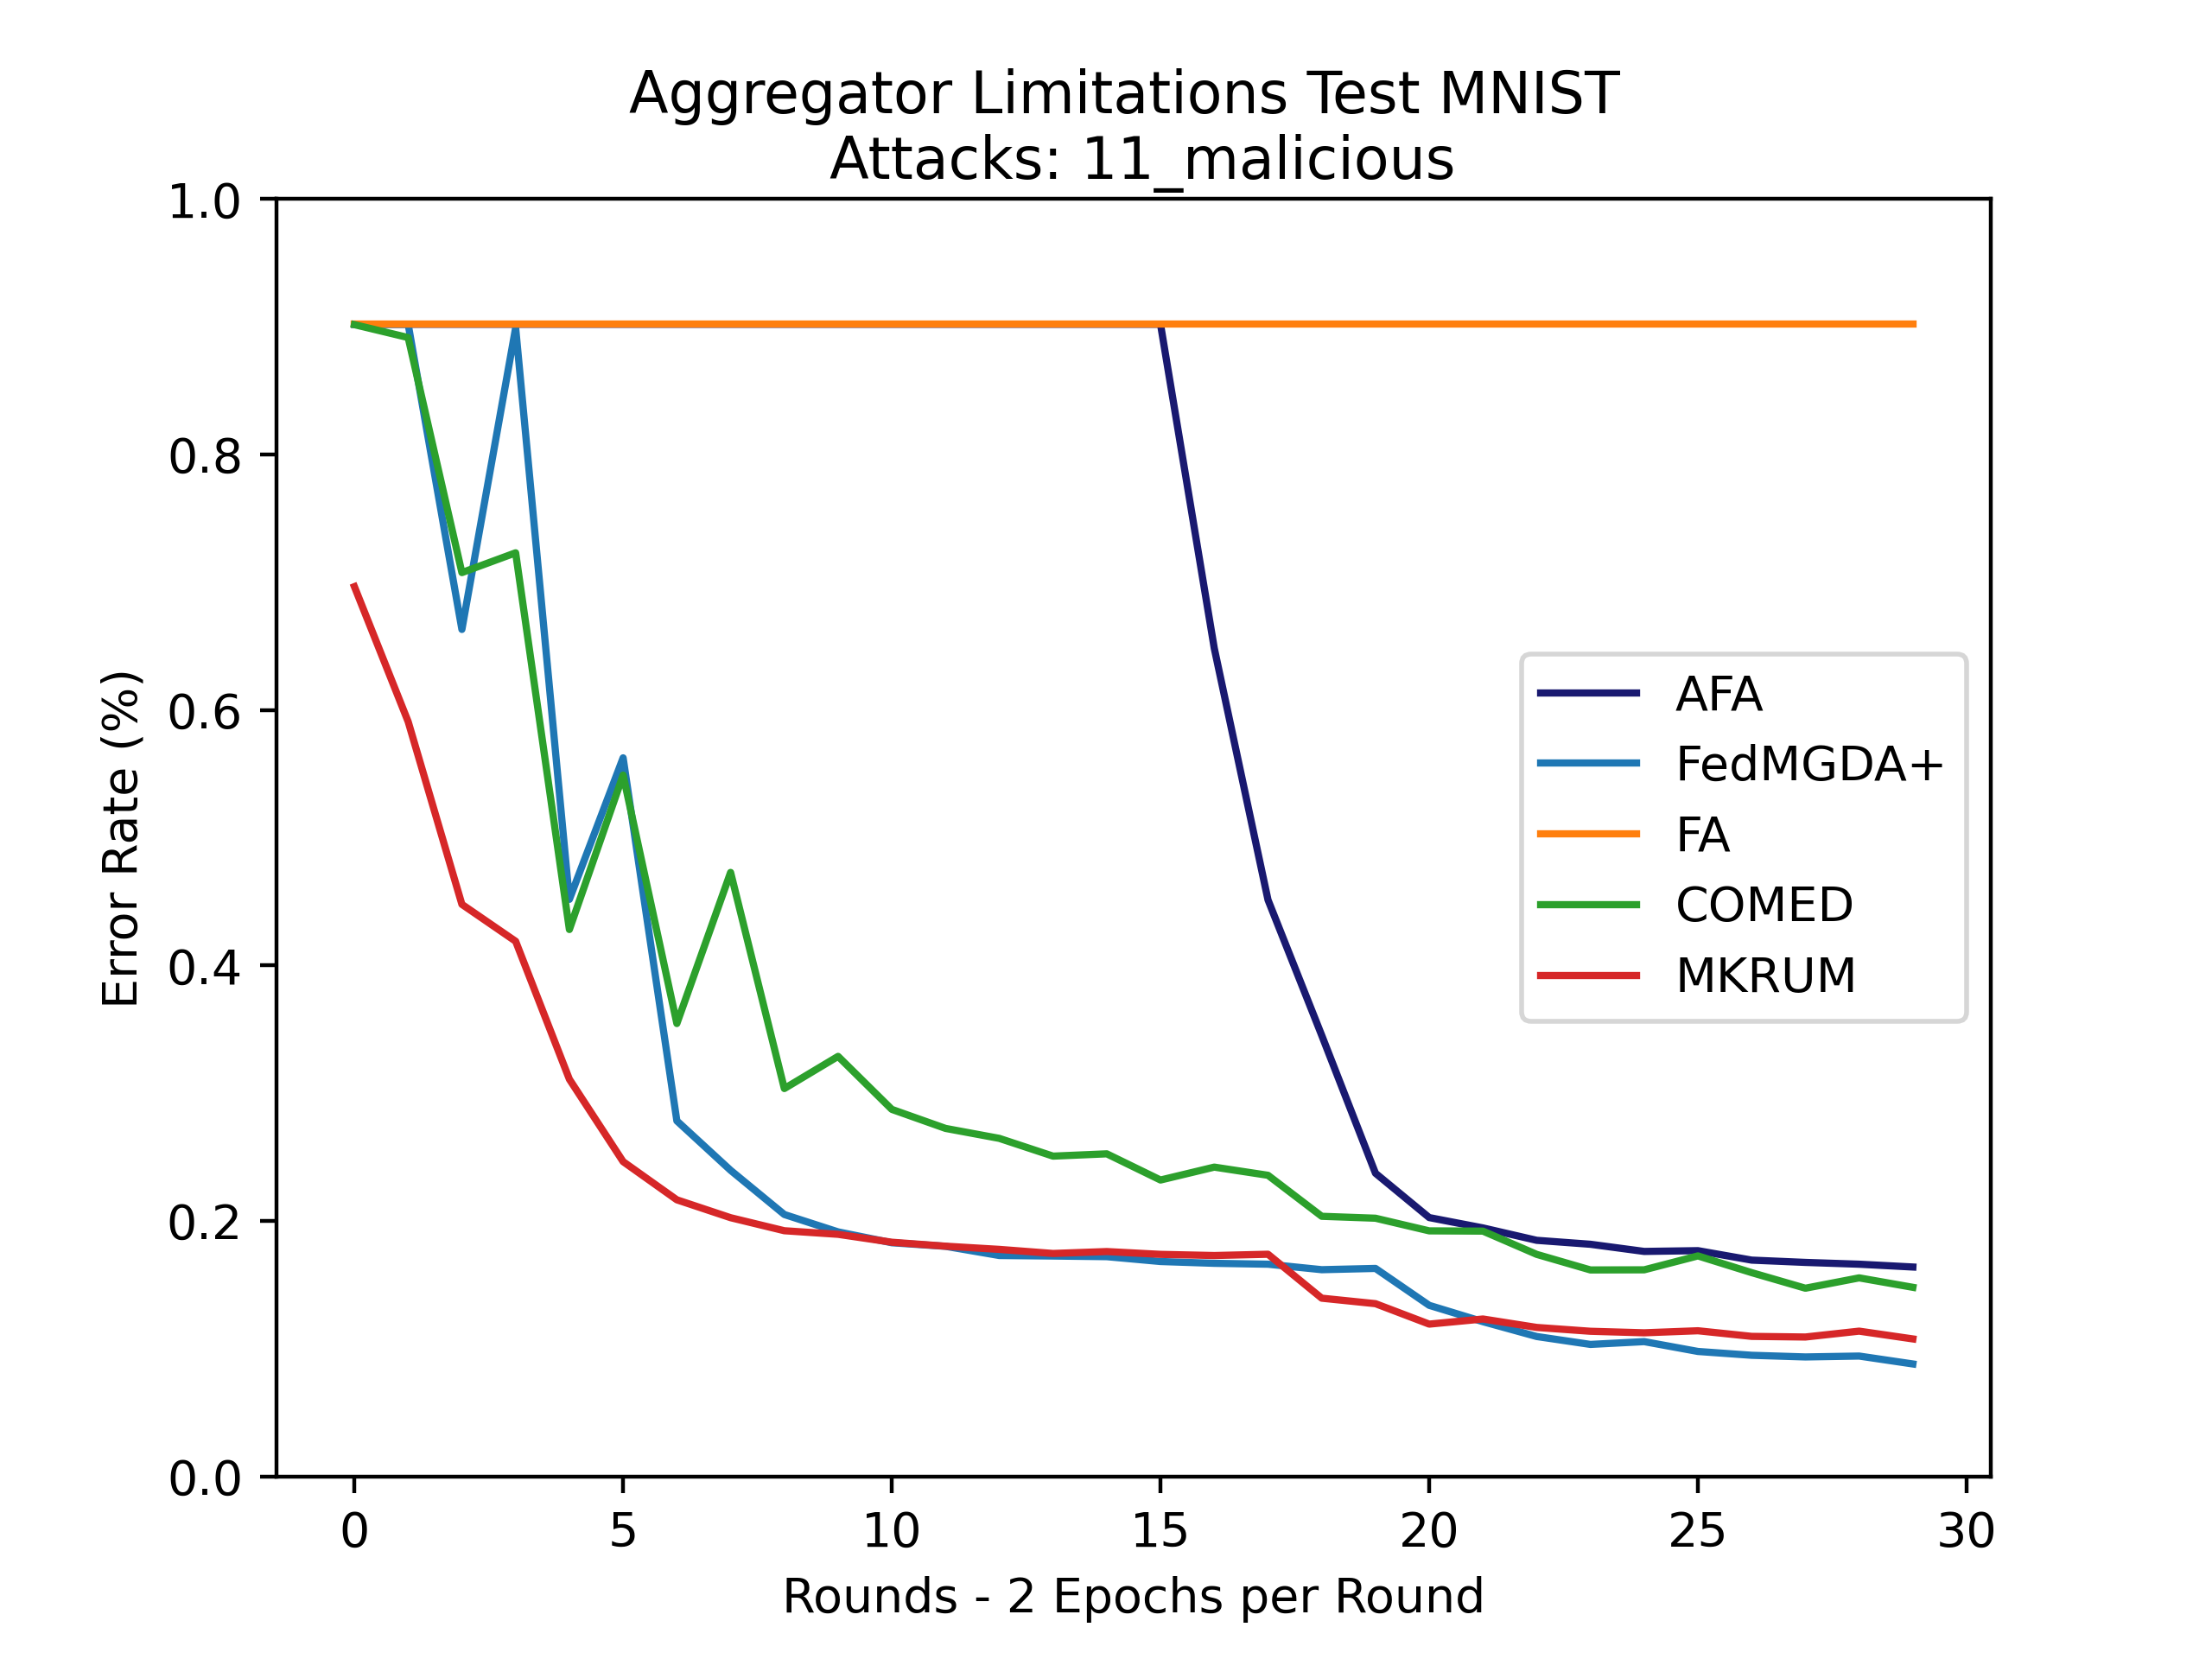
\includegraphics[scale=0.5]{initial/graphs/11_malicious.png}
	\caption{The Beginning of the End for Robust Aggregators with Malicious Clients}
	\label{fig:11mal}
\end{figure}

\begin{figure}[htbp]
	\centering
    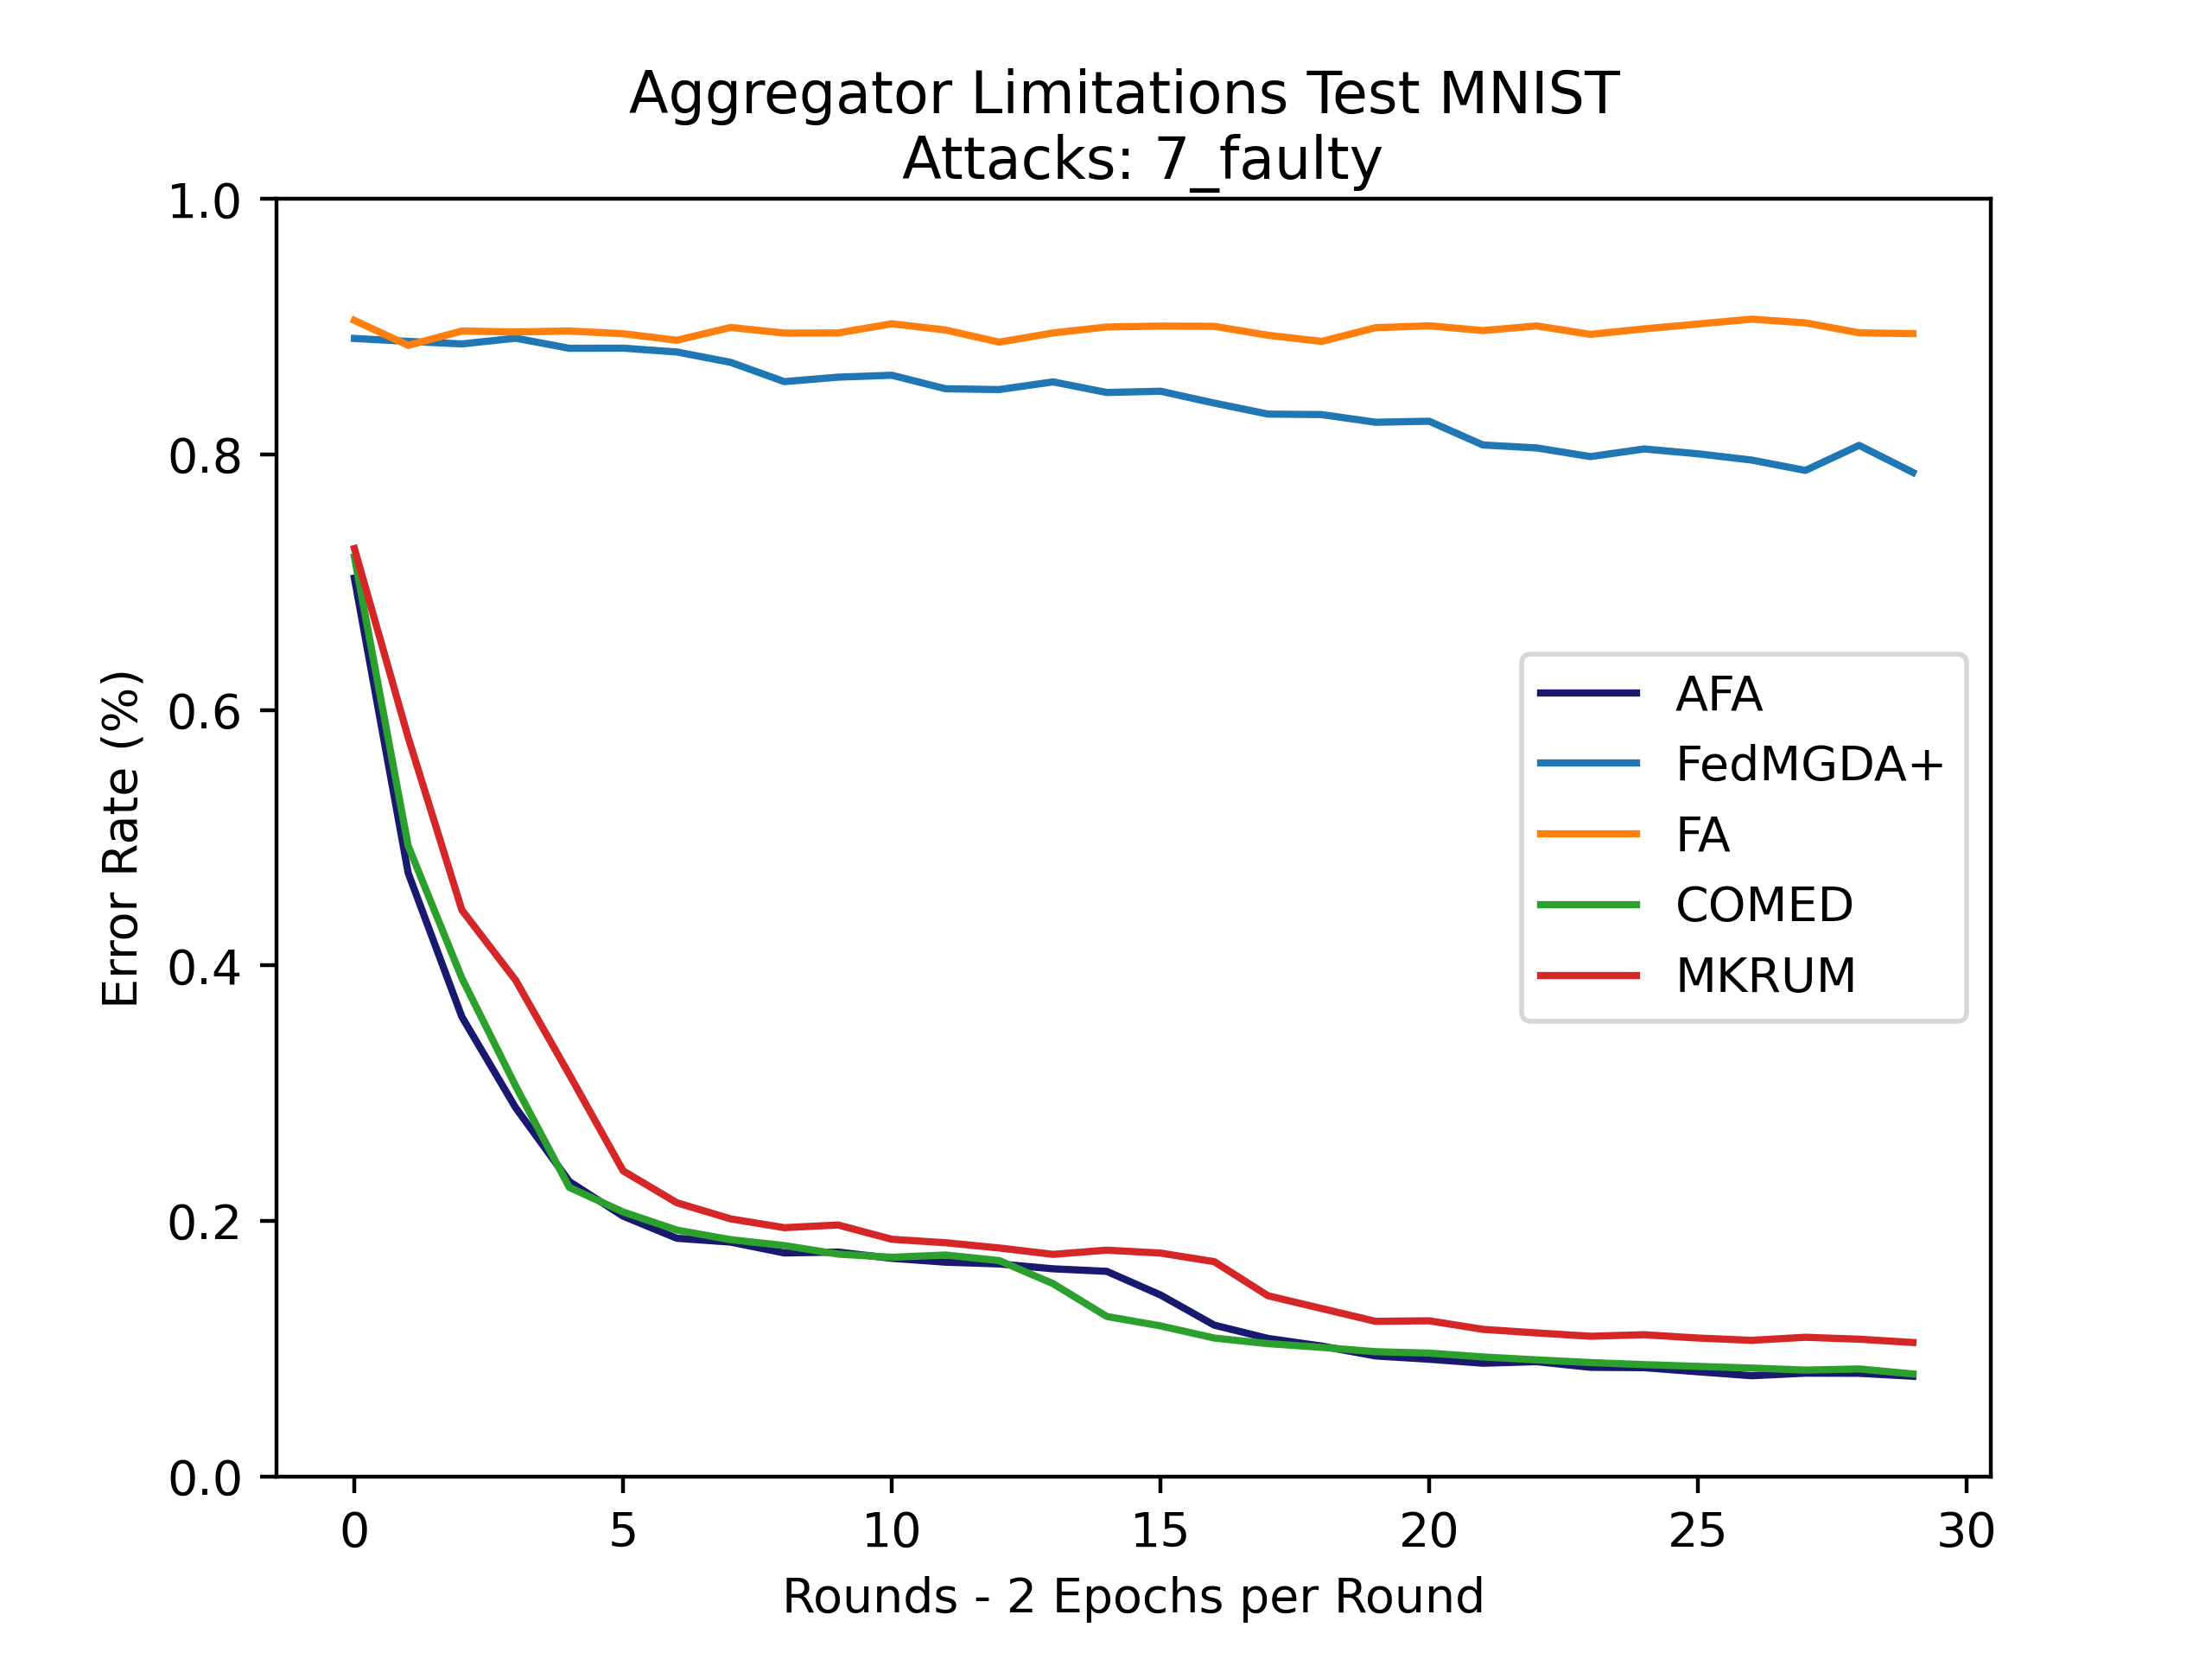
\includegraphics[scale=0.5]{initial/graphs/7_faulty.png}
	\caption{Slow Learning from FedMGDA++}
	\label{fig:7faulty}
\end{figure}

\begin{figure}[htbp]
	\centering
    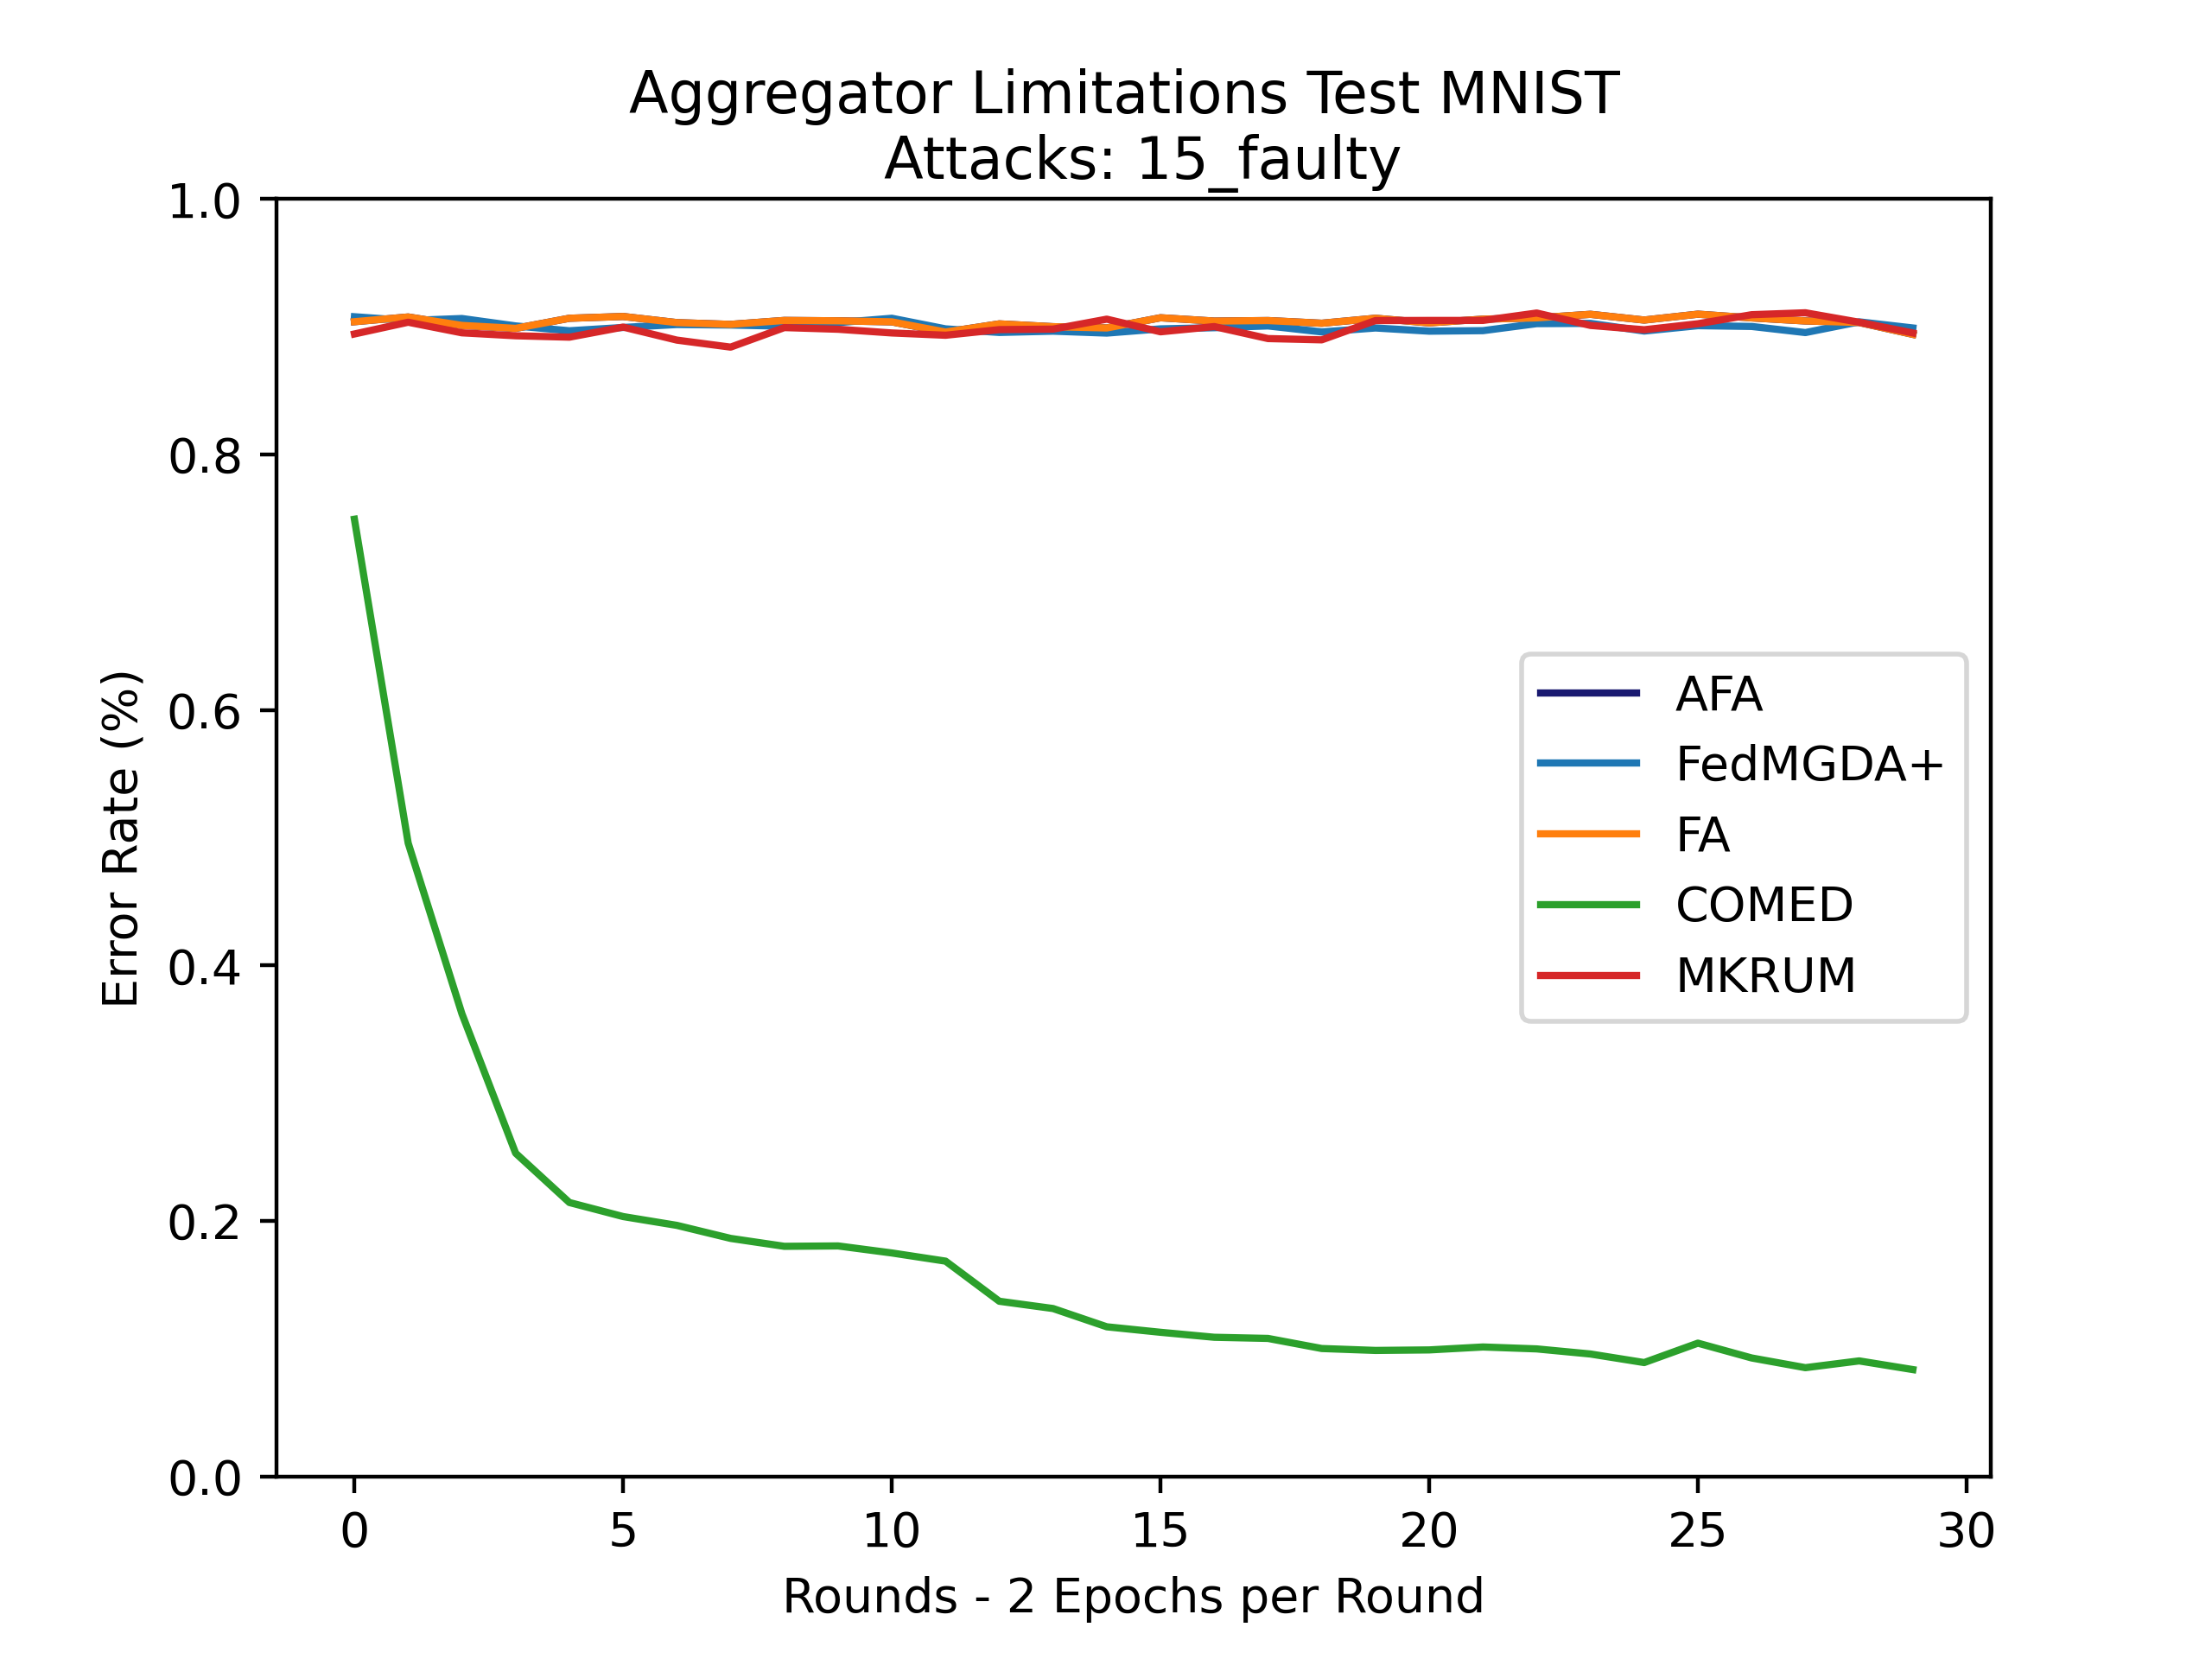
\includegraphics[scale=0.5]{initial/graphs/15_faulty.png}
	\caption{Attempts to Still Learn from Broken Aggregators}
	\label{fig:15faulty}
\end{figure}



\chapter{Free-Rider Investigations}
\begin{figure}[htbp]
	\centering
    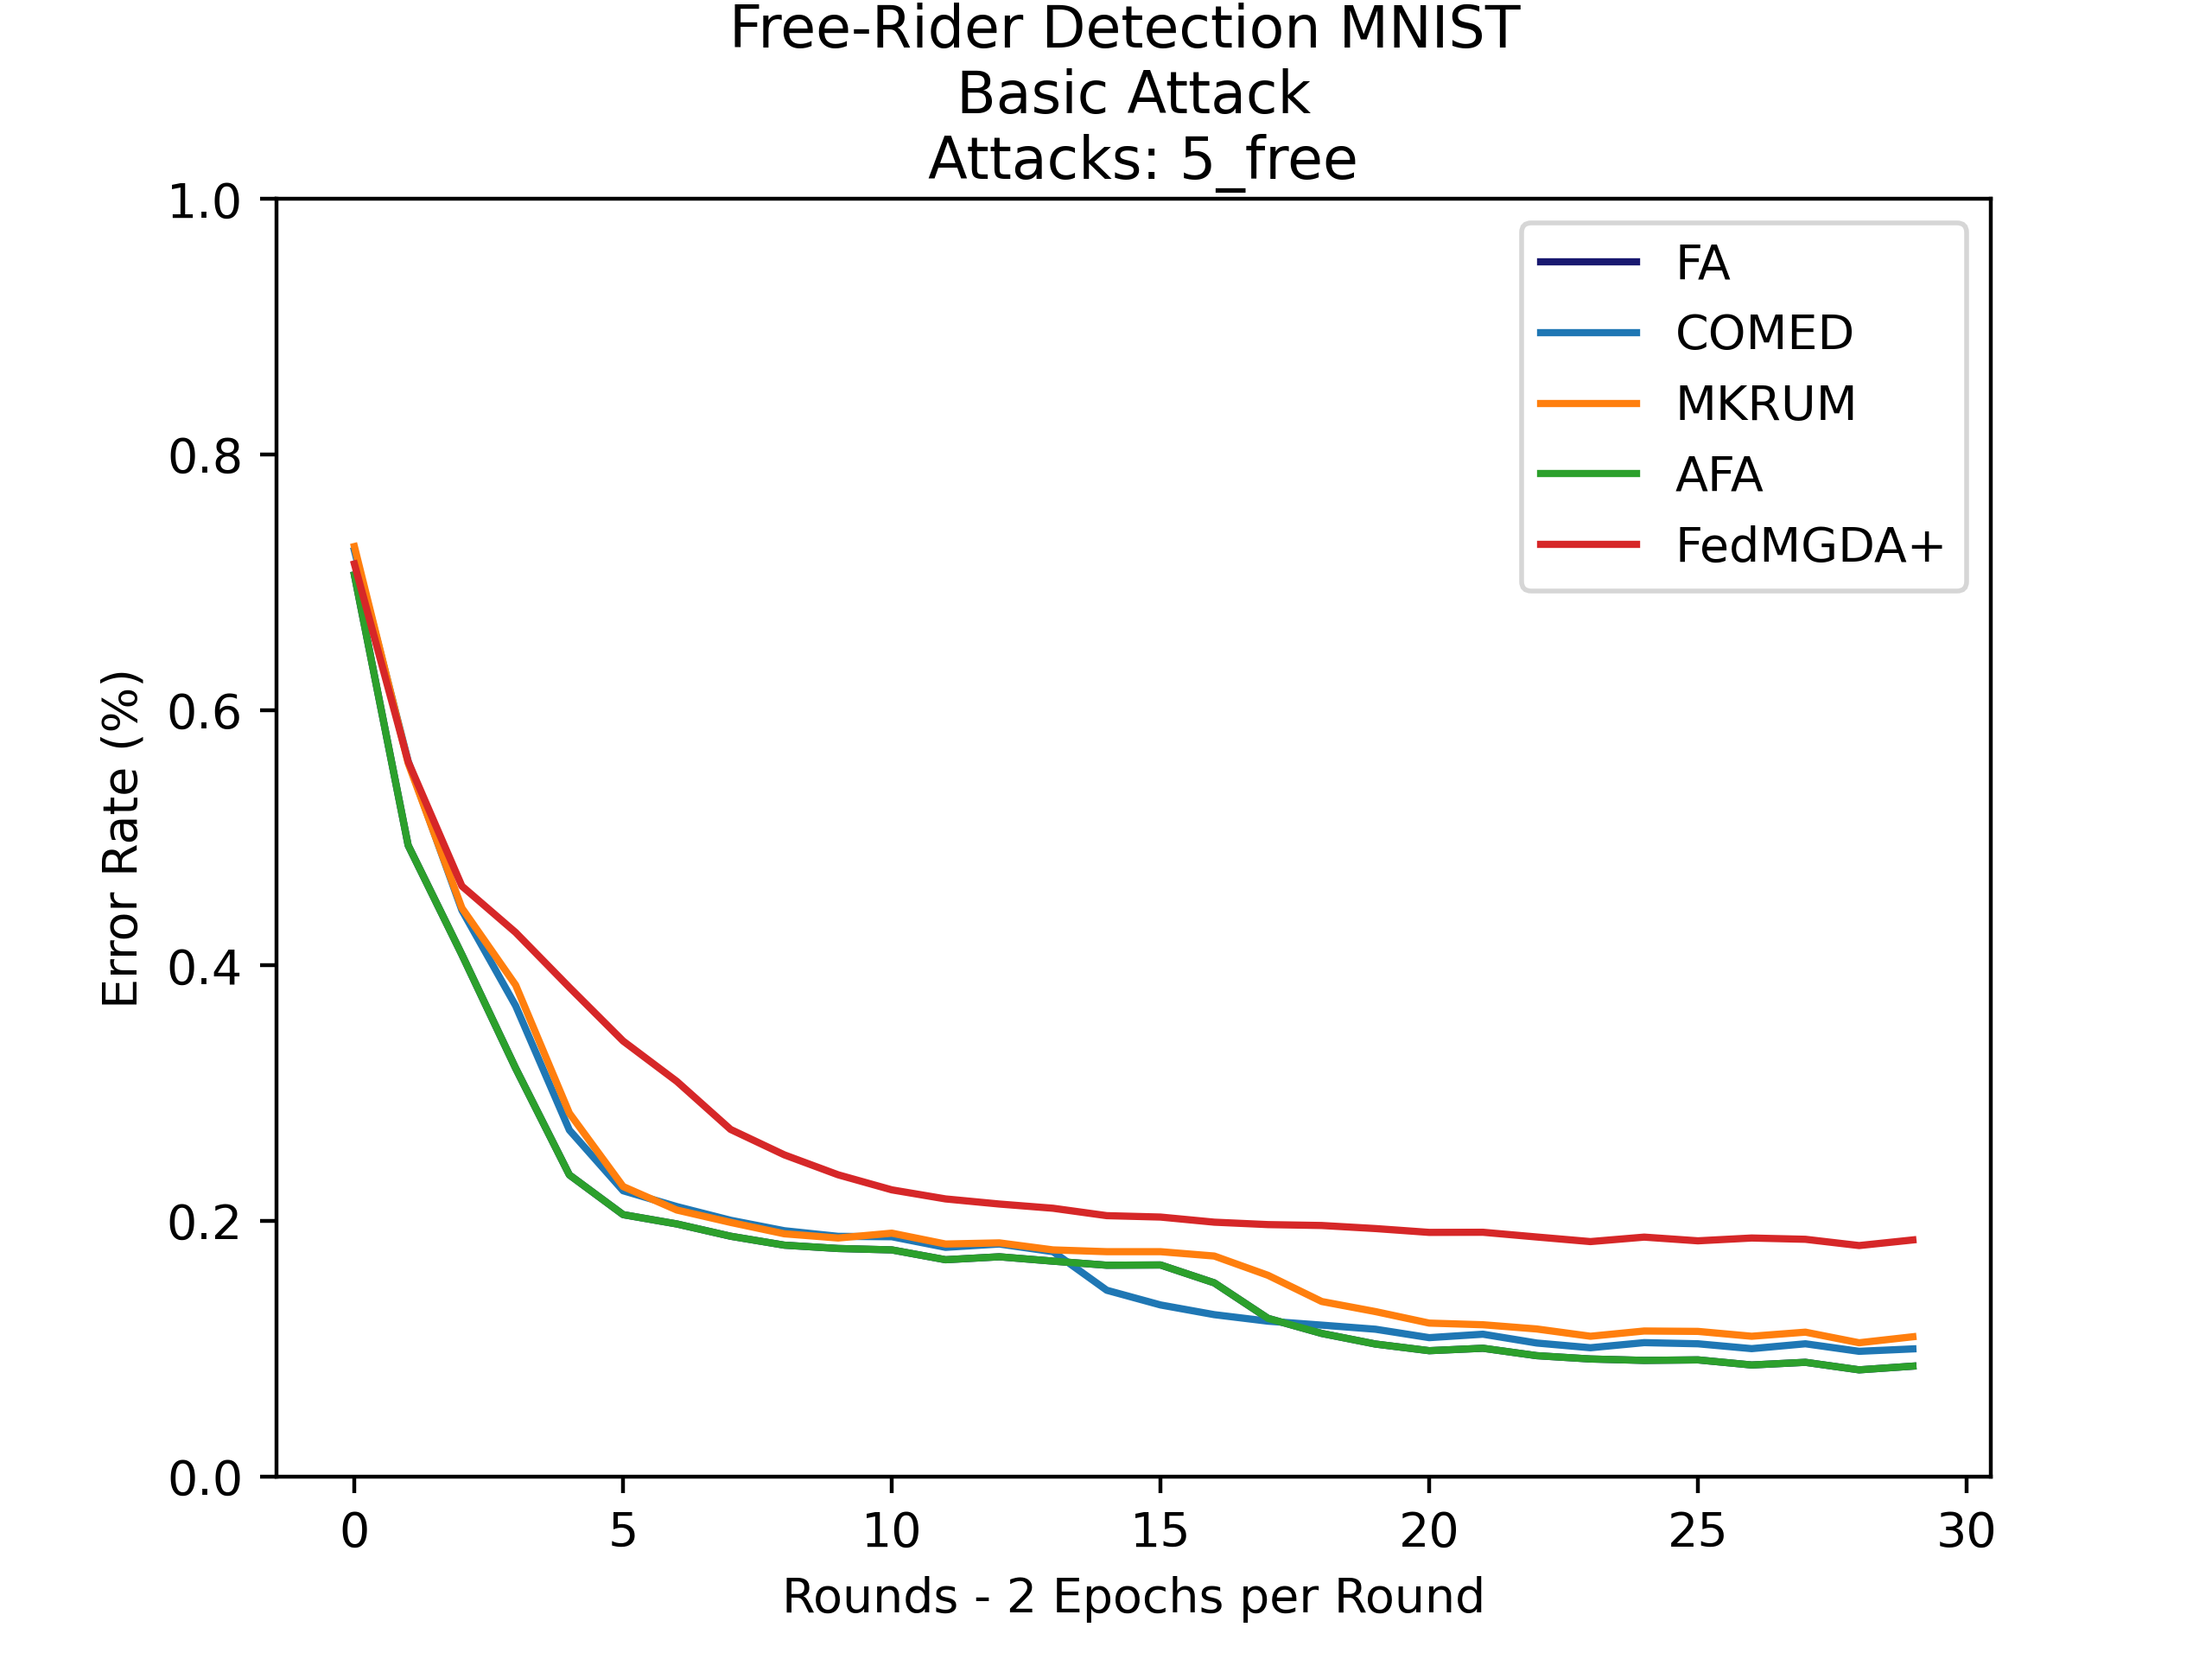
\includegraphics[scale=0.5]{free_riders/graphs/basic5.png}
	\caption{Basic Attack with 5 Free-Riders - Basically No Damage Done}
	\label{fig:5free}
\end{figure}

\begin{figure}[htbp]
	\centering
    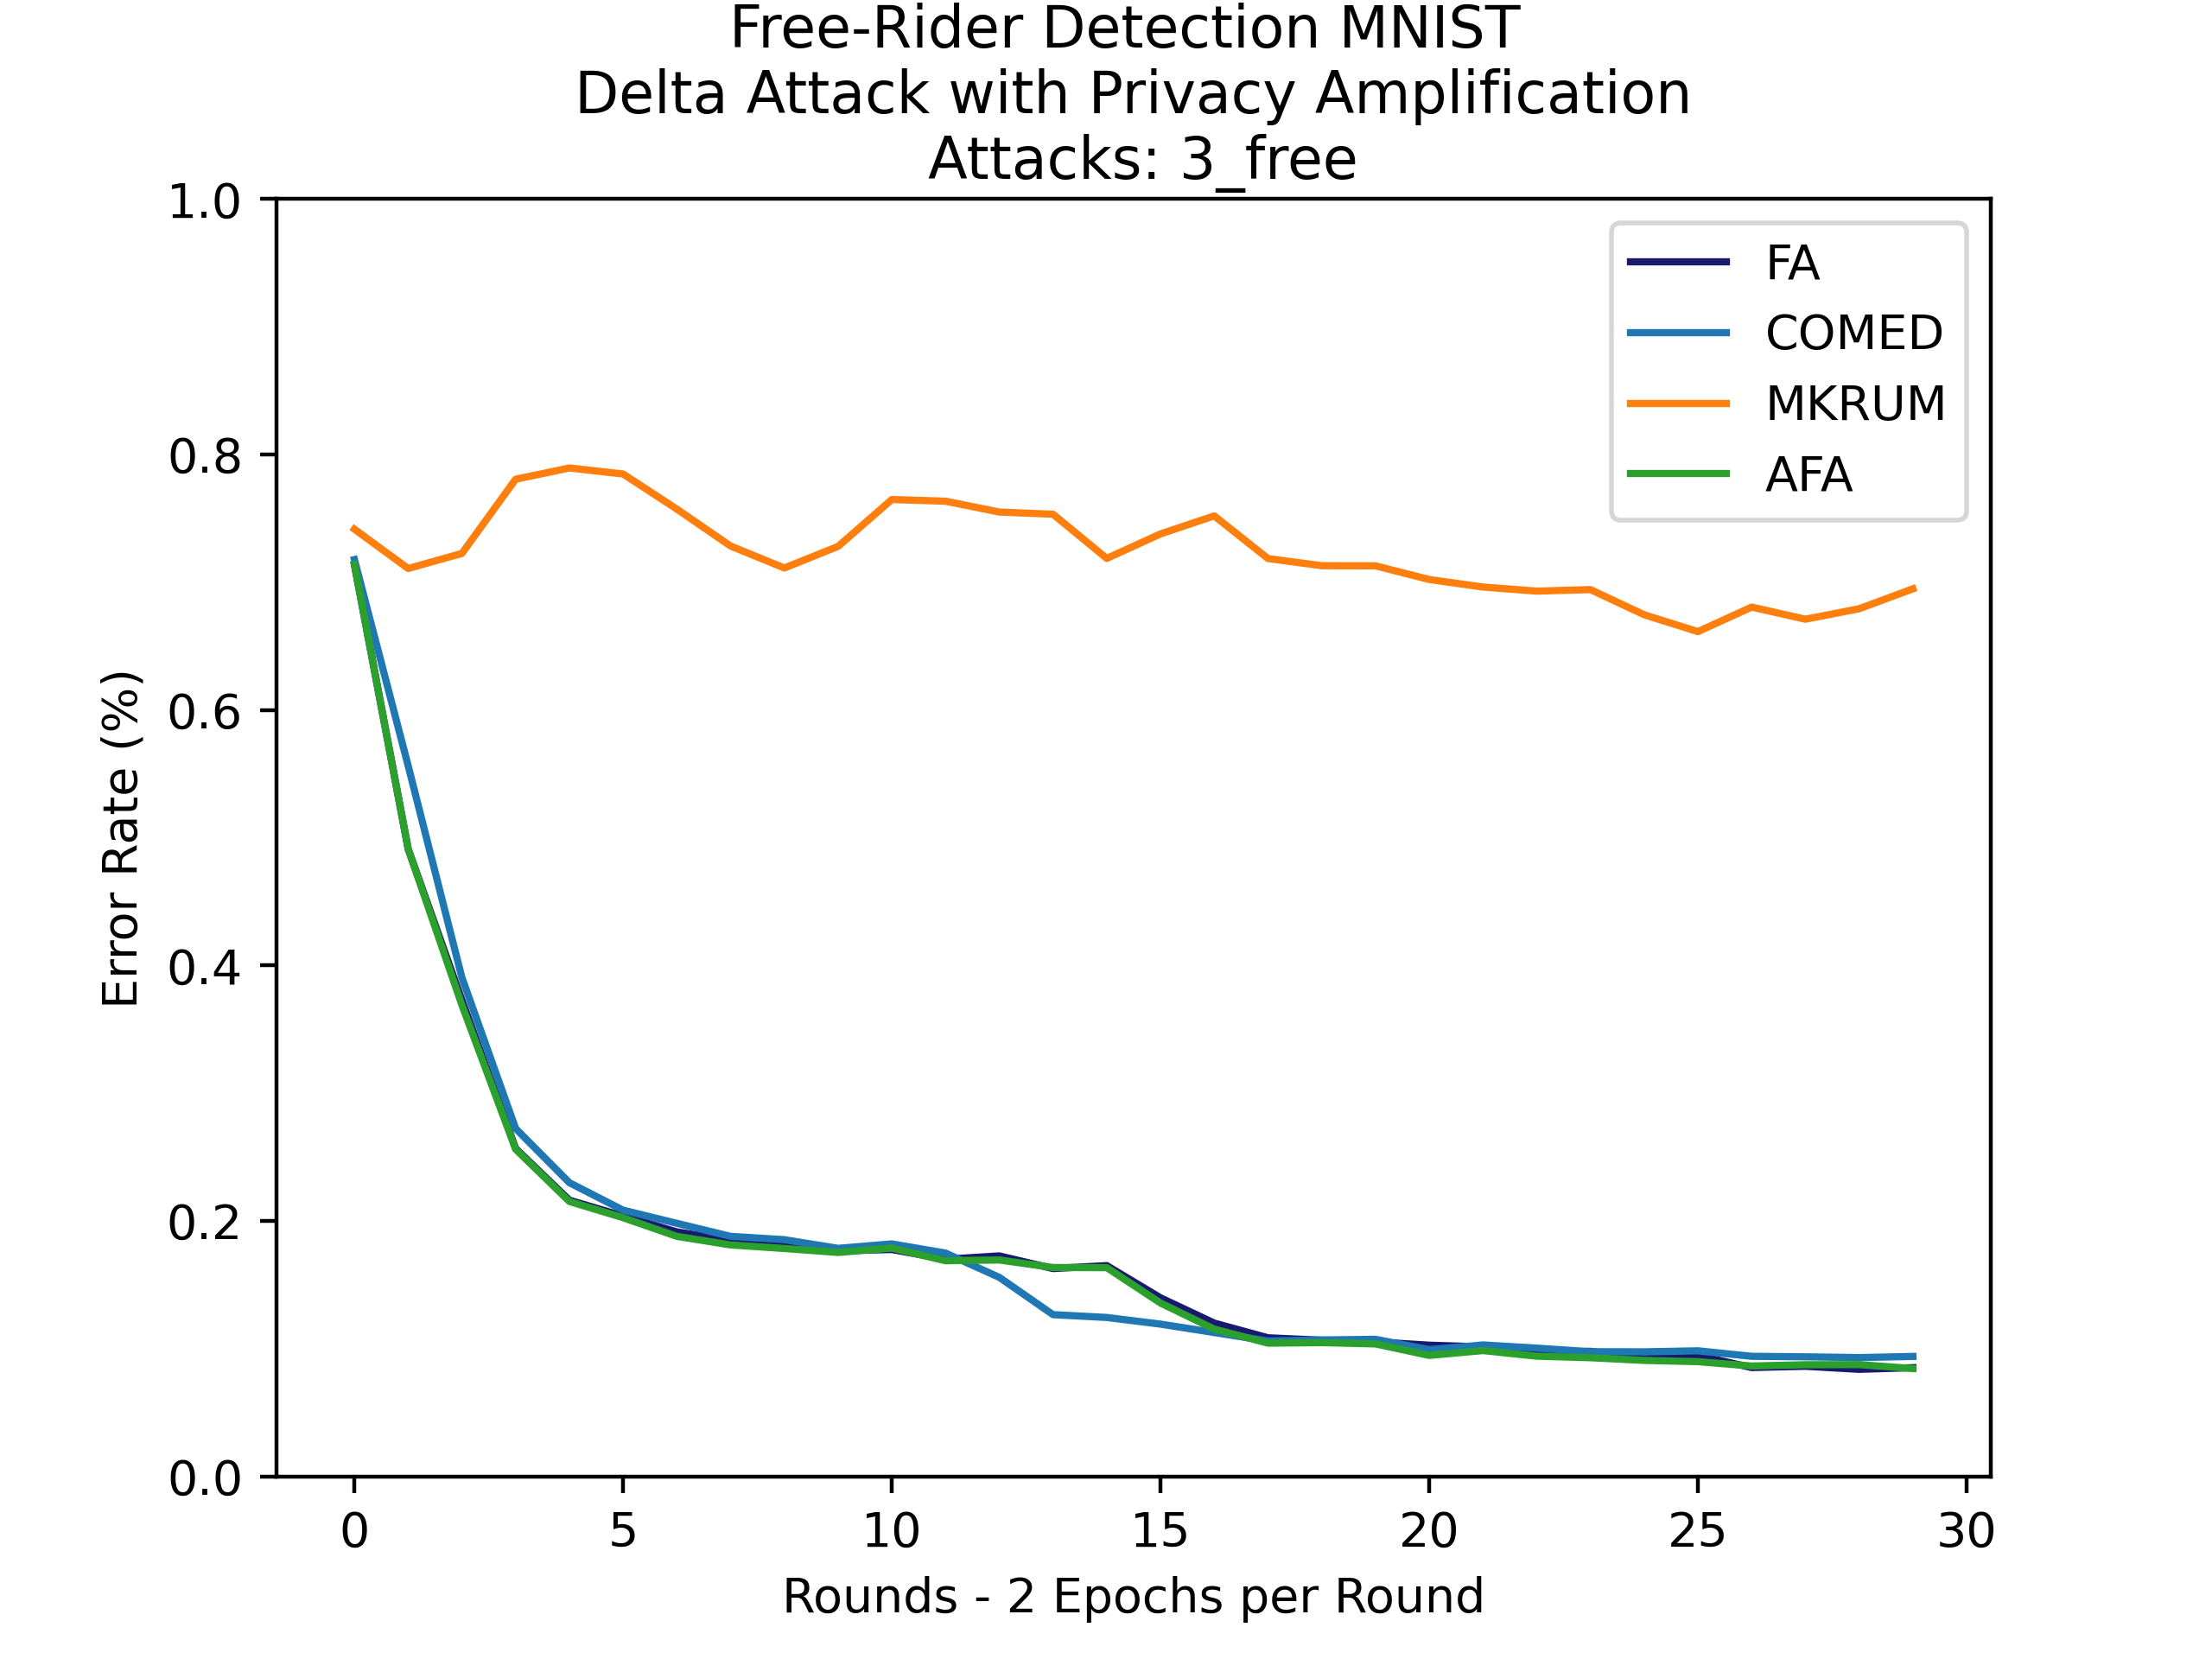
\includegraphics[scale=0.5]{free_riders/graphs/mkrum_suffer.png}
	\caption{MKRUM Suffering with Only 3 Free-Riding Clients under Privacy Amplification with a Delta-Weight Attack}
	\label{fig:mkrum_suf}
\end{figure}

\begin{figure}[htbp]
	\centering
    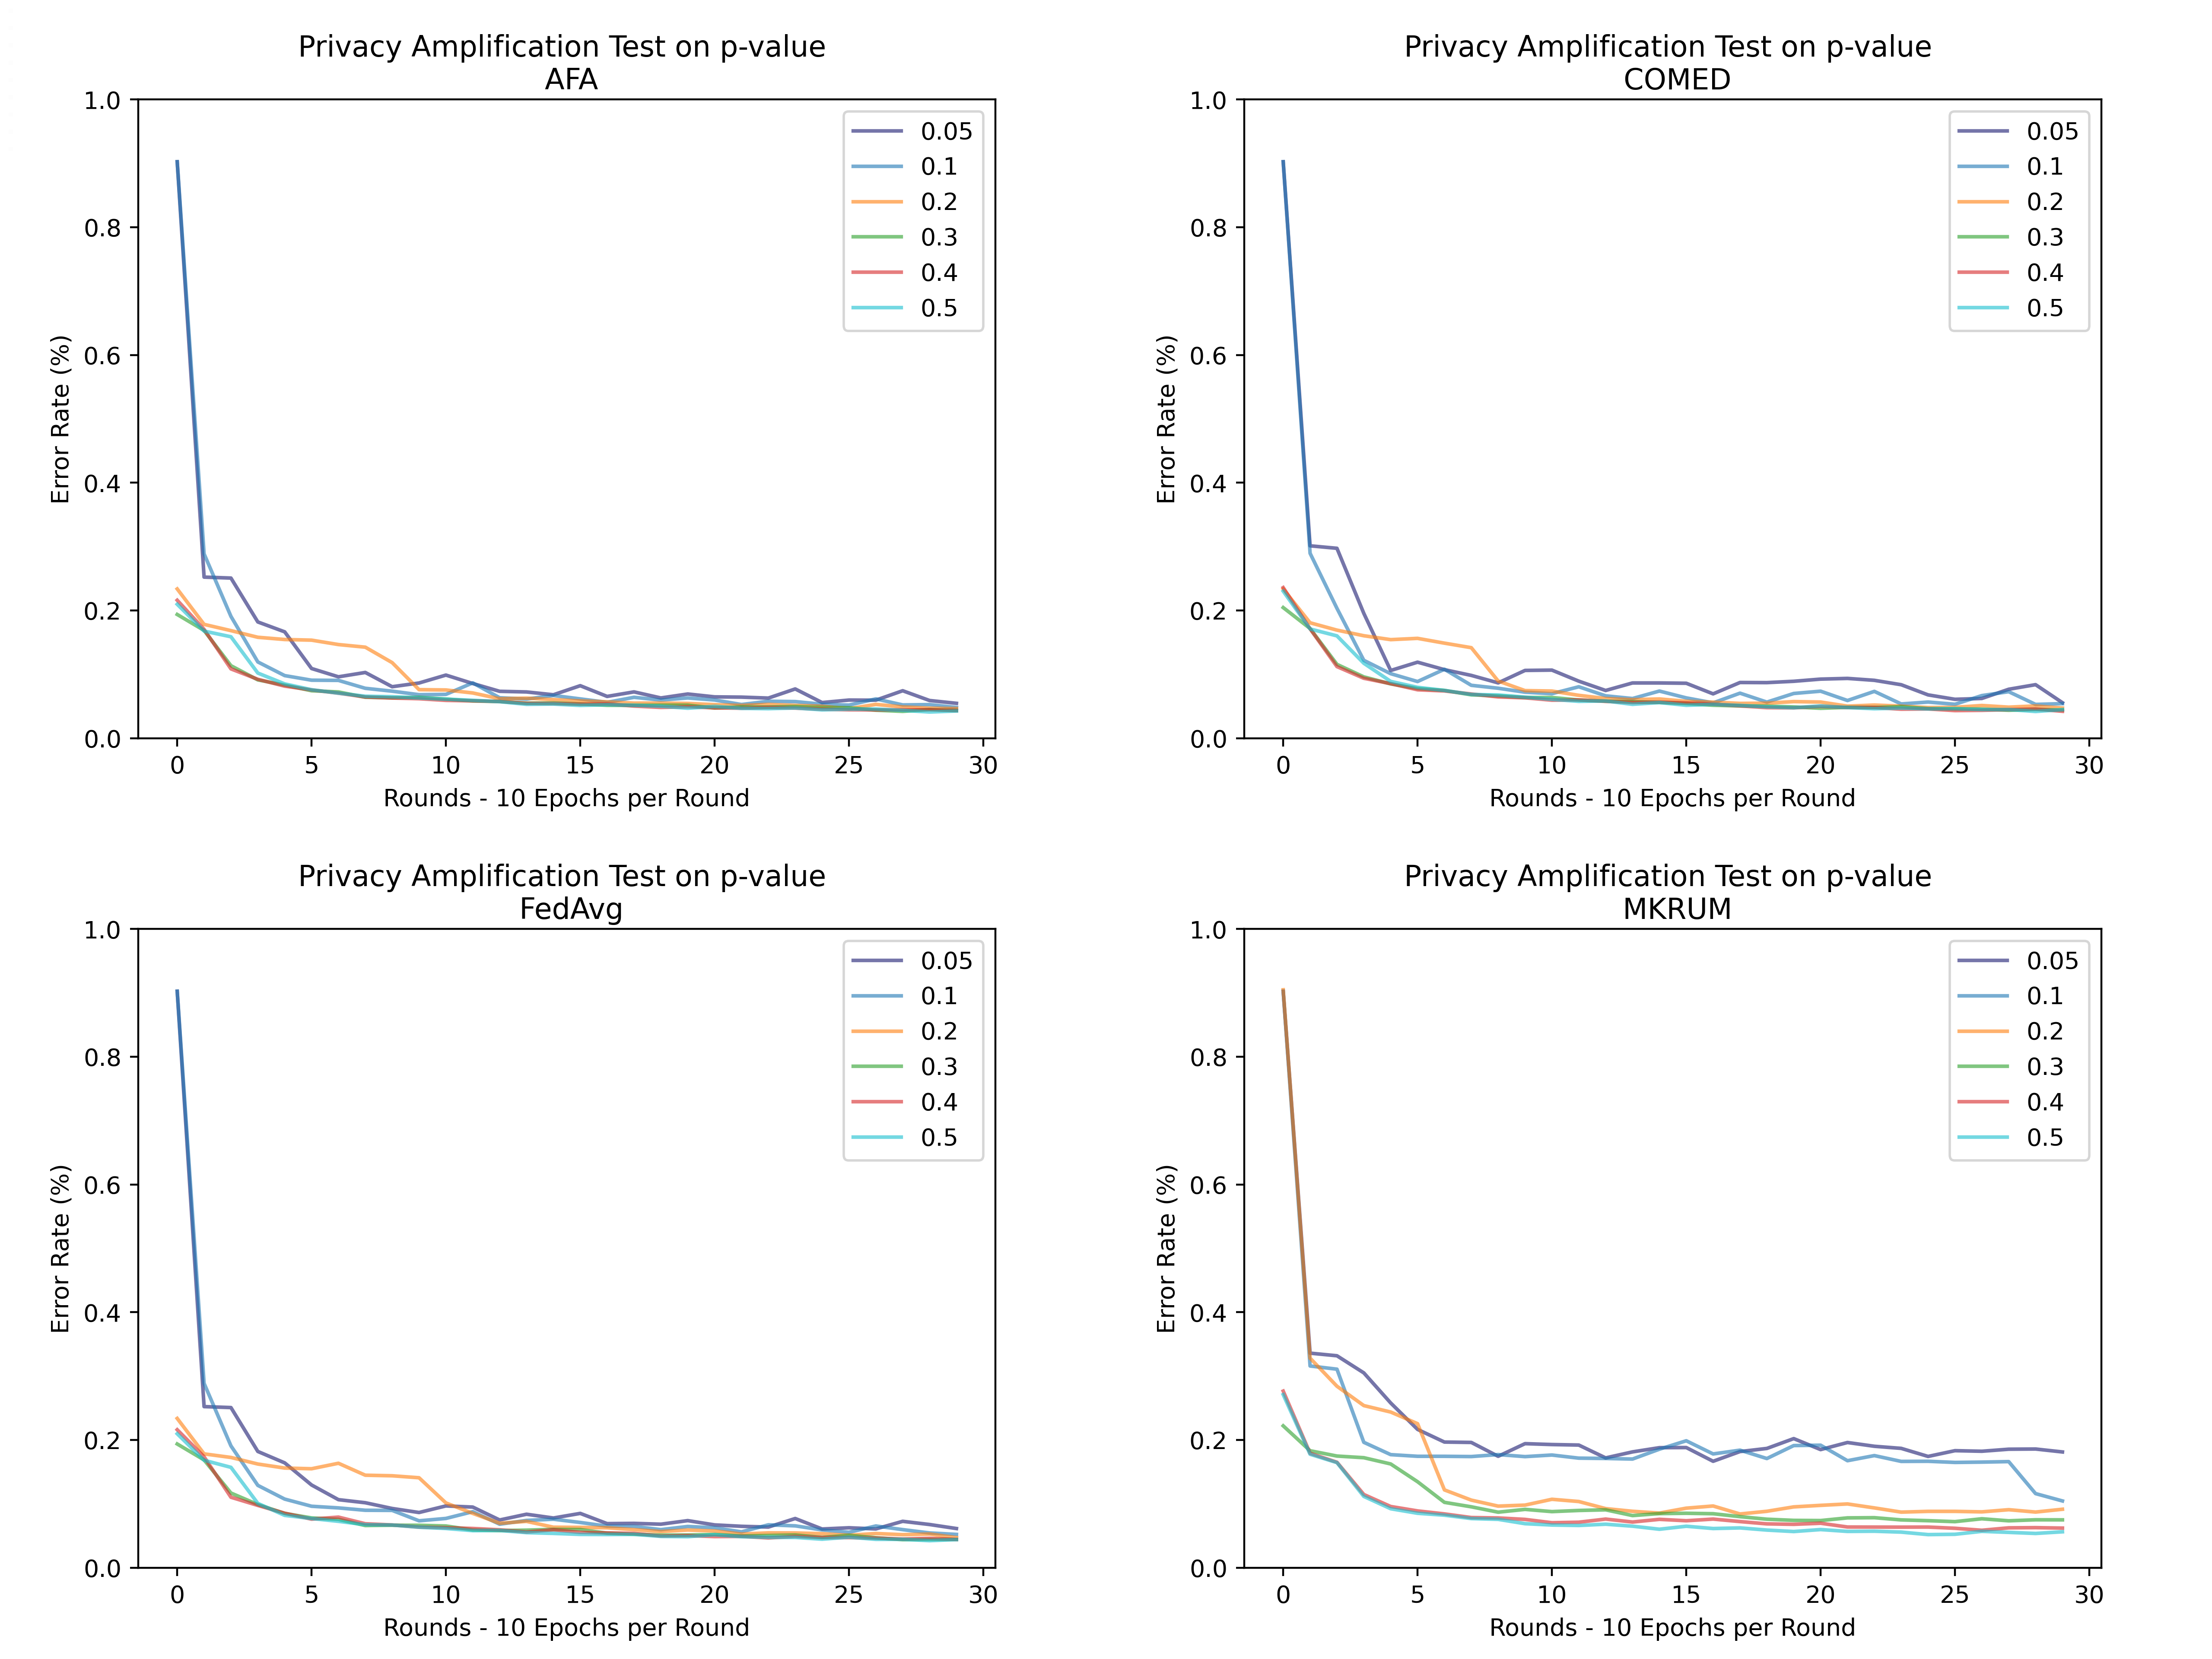
\includegraphics[scale=0.07]{free_riders/graphs/p_test.png}
	\caption{Privacy Amplification with Uniform Sampling with p-Thresholds - 10 epochs}
	\label{fig:p_test}
\end{figure}

\begin{figure}[htbp]
	\centering
    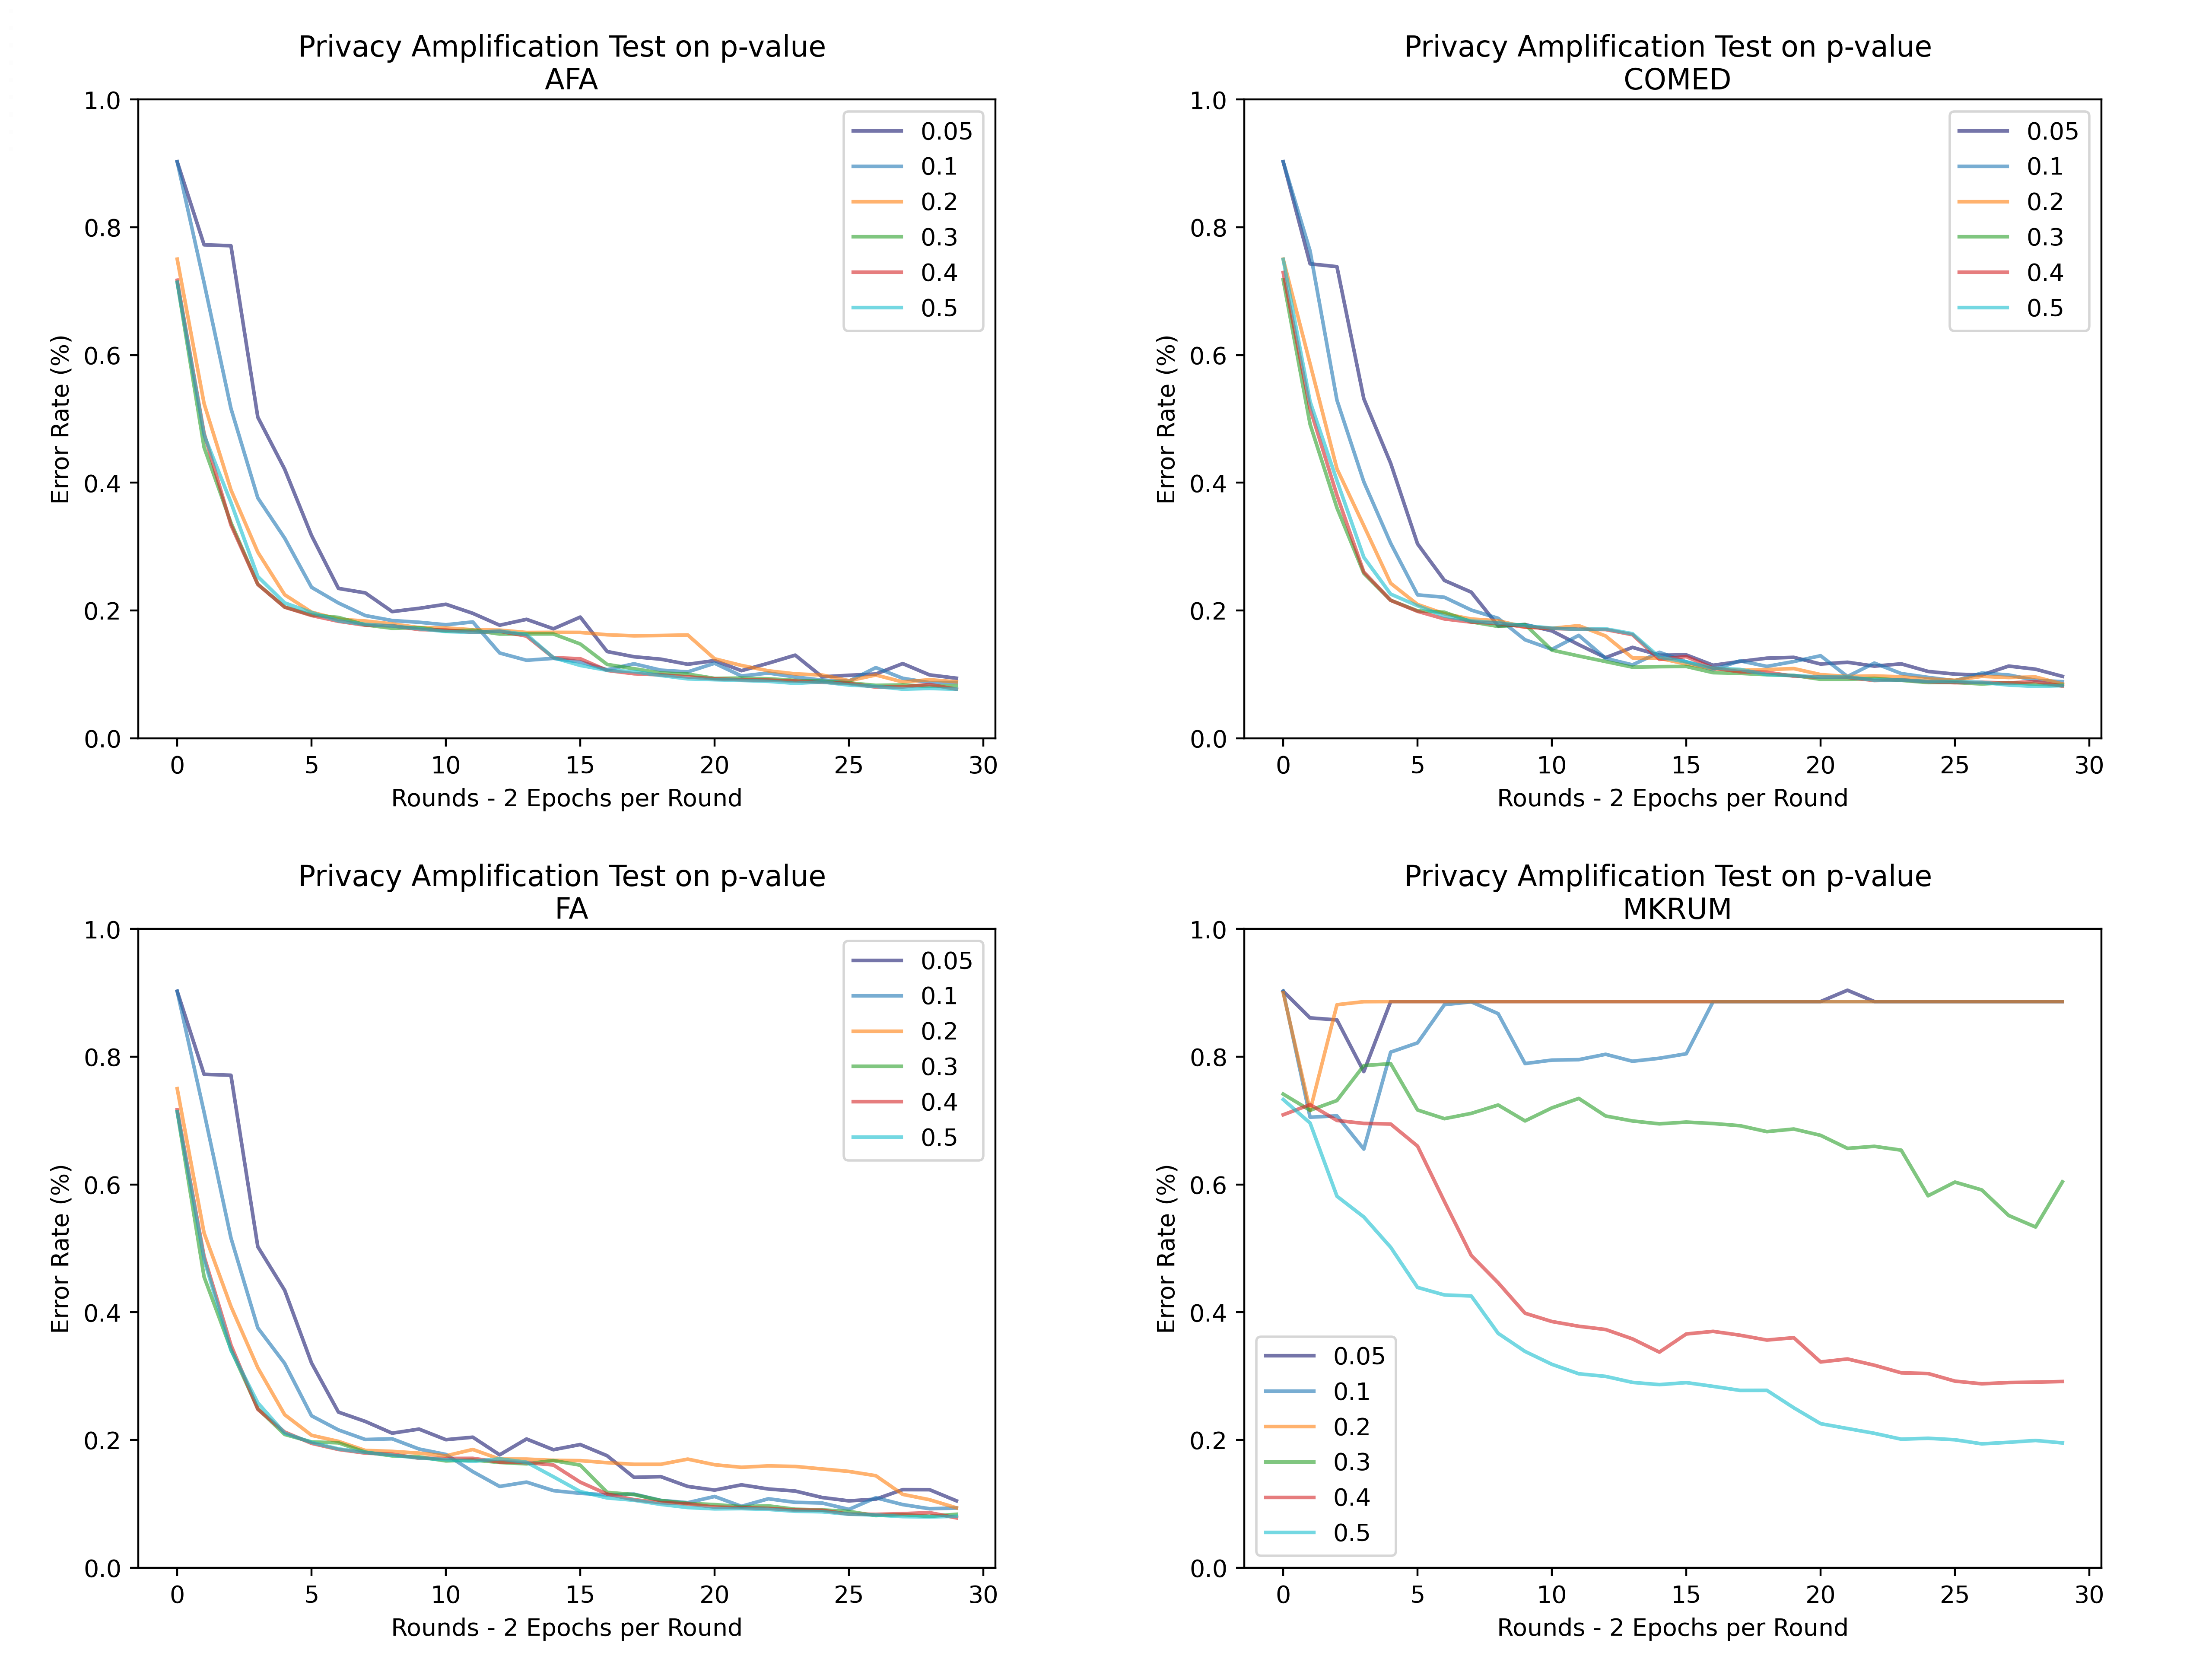
\includegraphics[scale=0.07]{free_riders/graphs/p_test_2.png}
	\caption{Privacy Amplification with Uniform Sampling with p-Thresholds - 2 epochs}
	\label{fig:p_test_2}
\end{figure}

\begin{figure}[htbp]
	\centering
    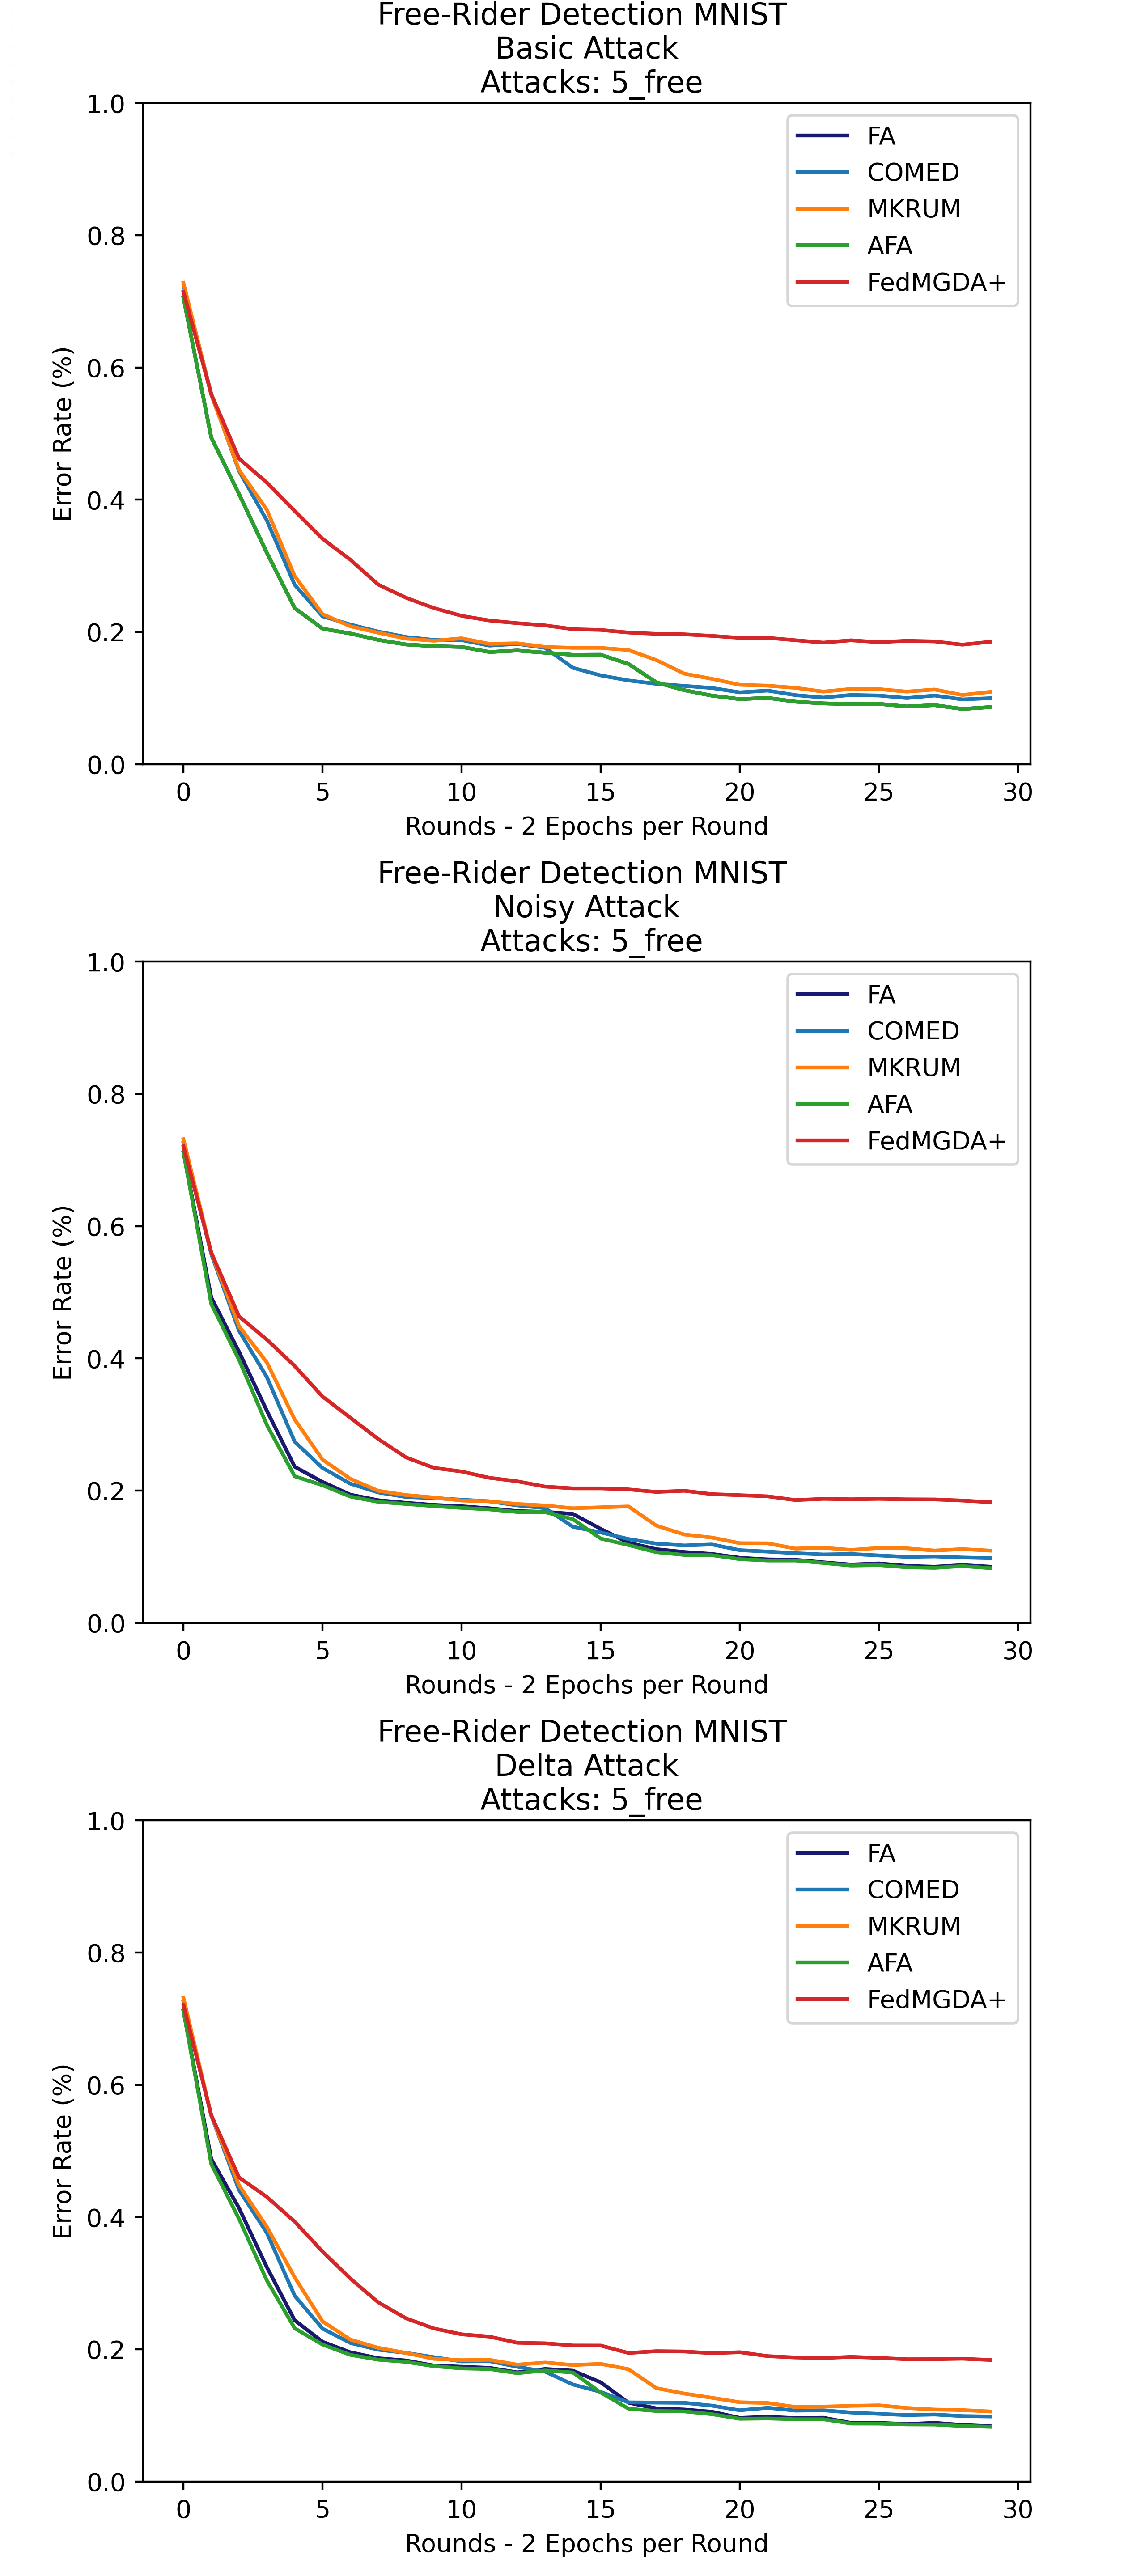
\includegraphics[scale=0.1]{free_riders/graphs/no_dmg.png}
	\caption{Minimal Performance Degradation with 5 Free-Riders}
	\label{fig:no_dmg}
\end{figure}

\begin{figure}[htbp]
	\centering
    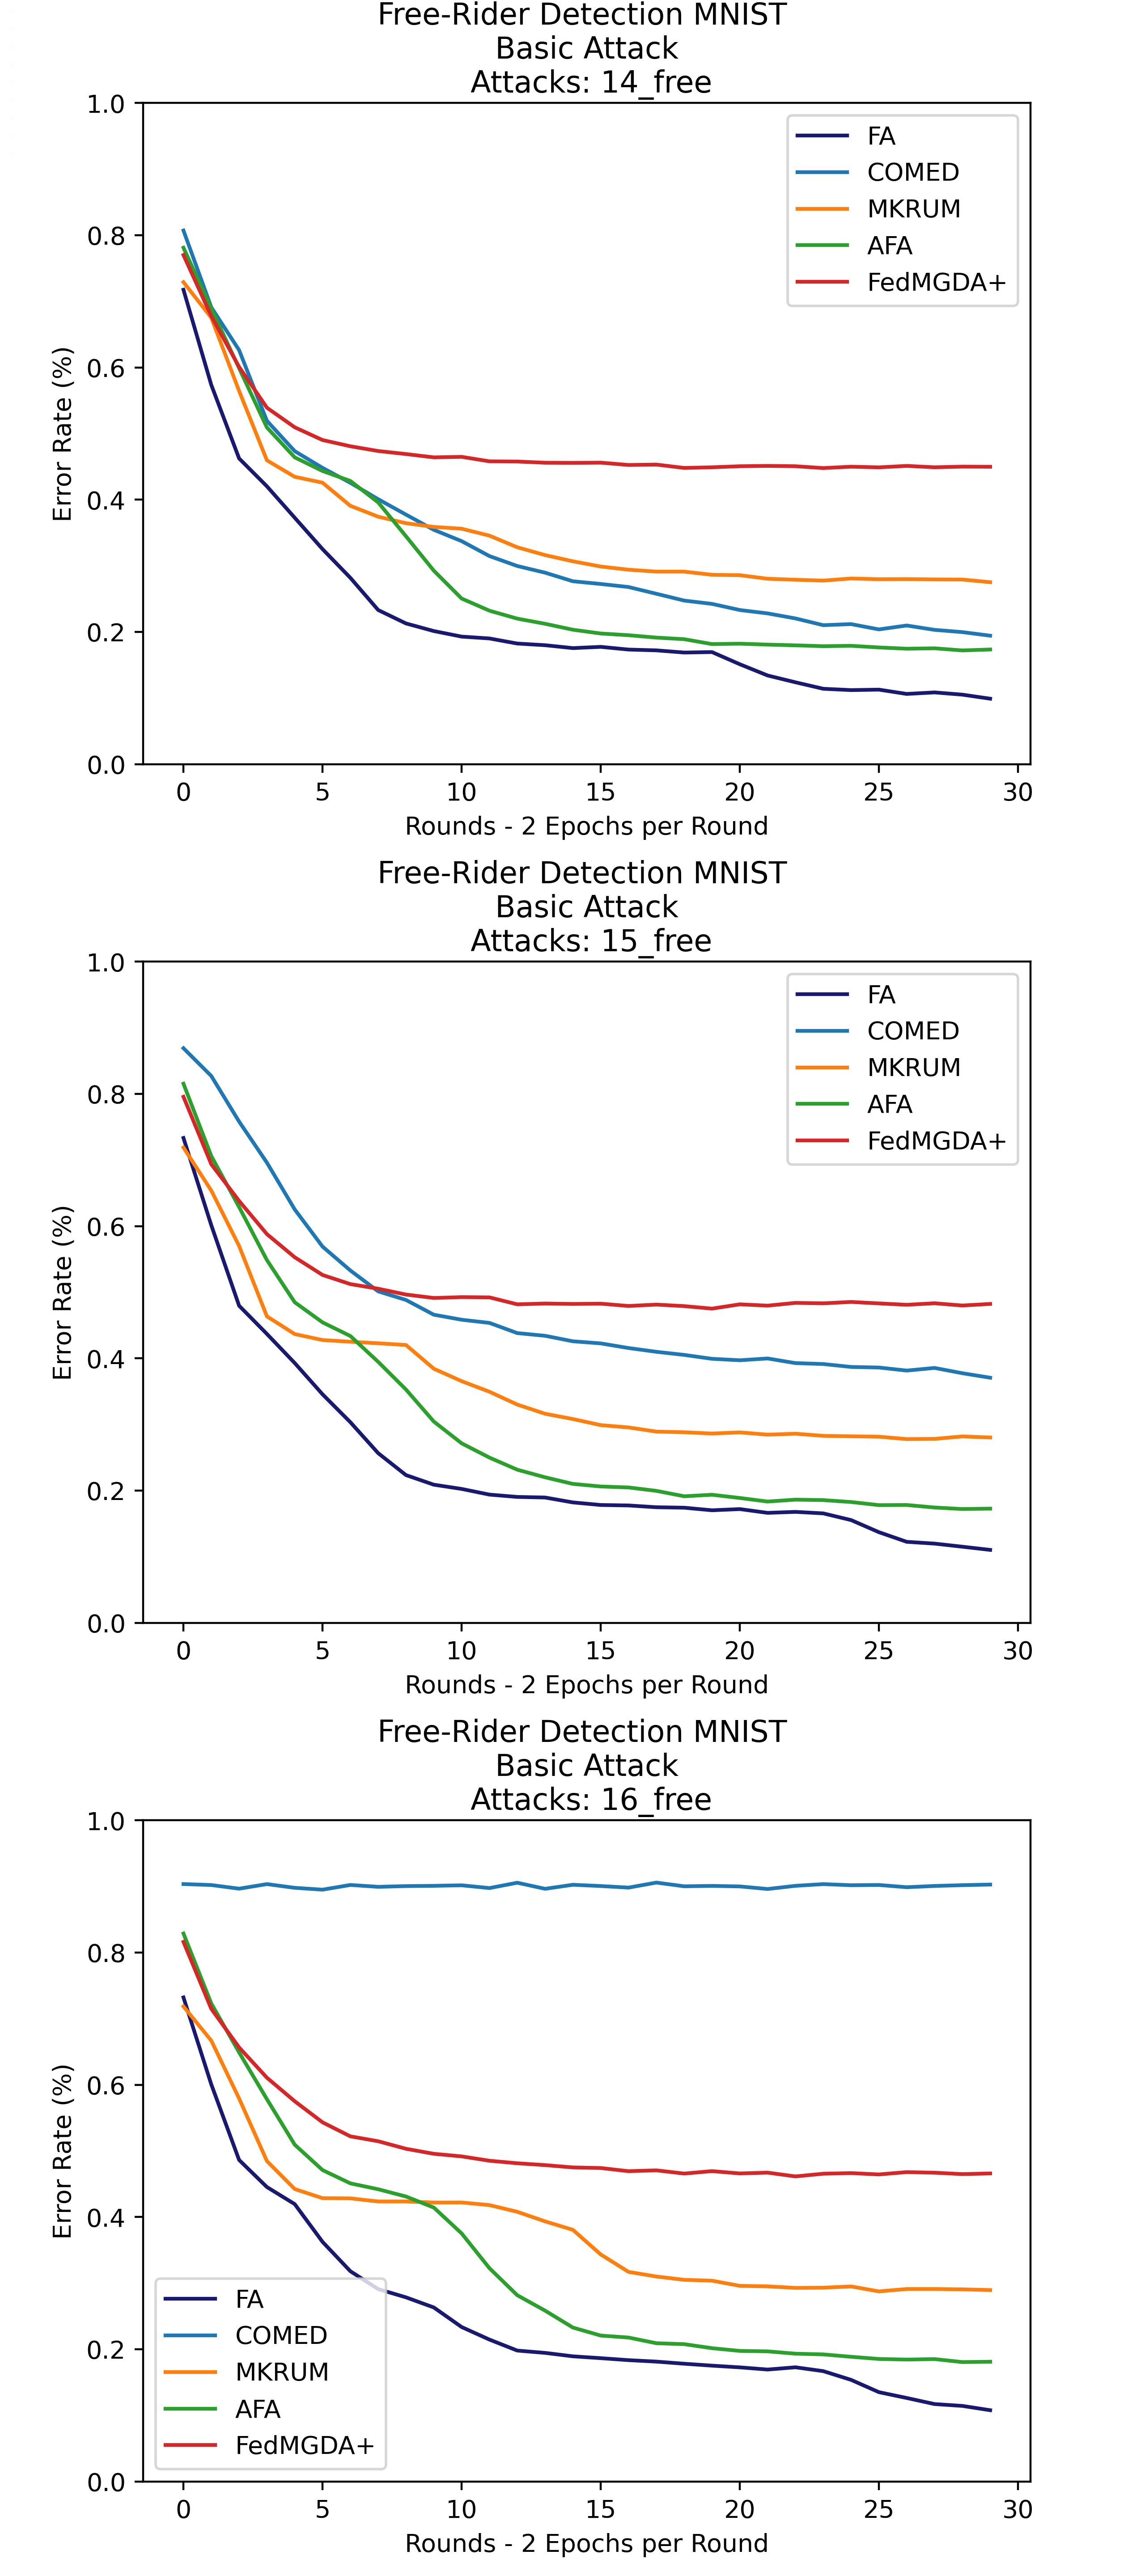
\includegraphics[scale=0.1]{free_riders/graphs/comed_broken.png}
	\caption{Transition of COMED's Error Rate Drastically Increasing as it Breaks the Threshold}
	\label{fig:comed_broken}
\end{figure}

\chapter{FedPADRC}
\begin{figure}[htbp]
	\centering
    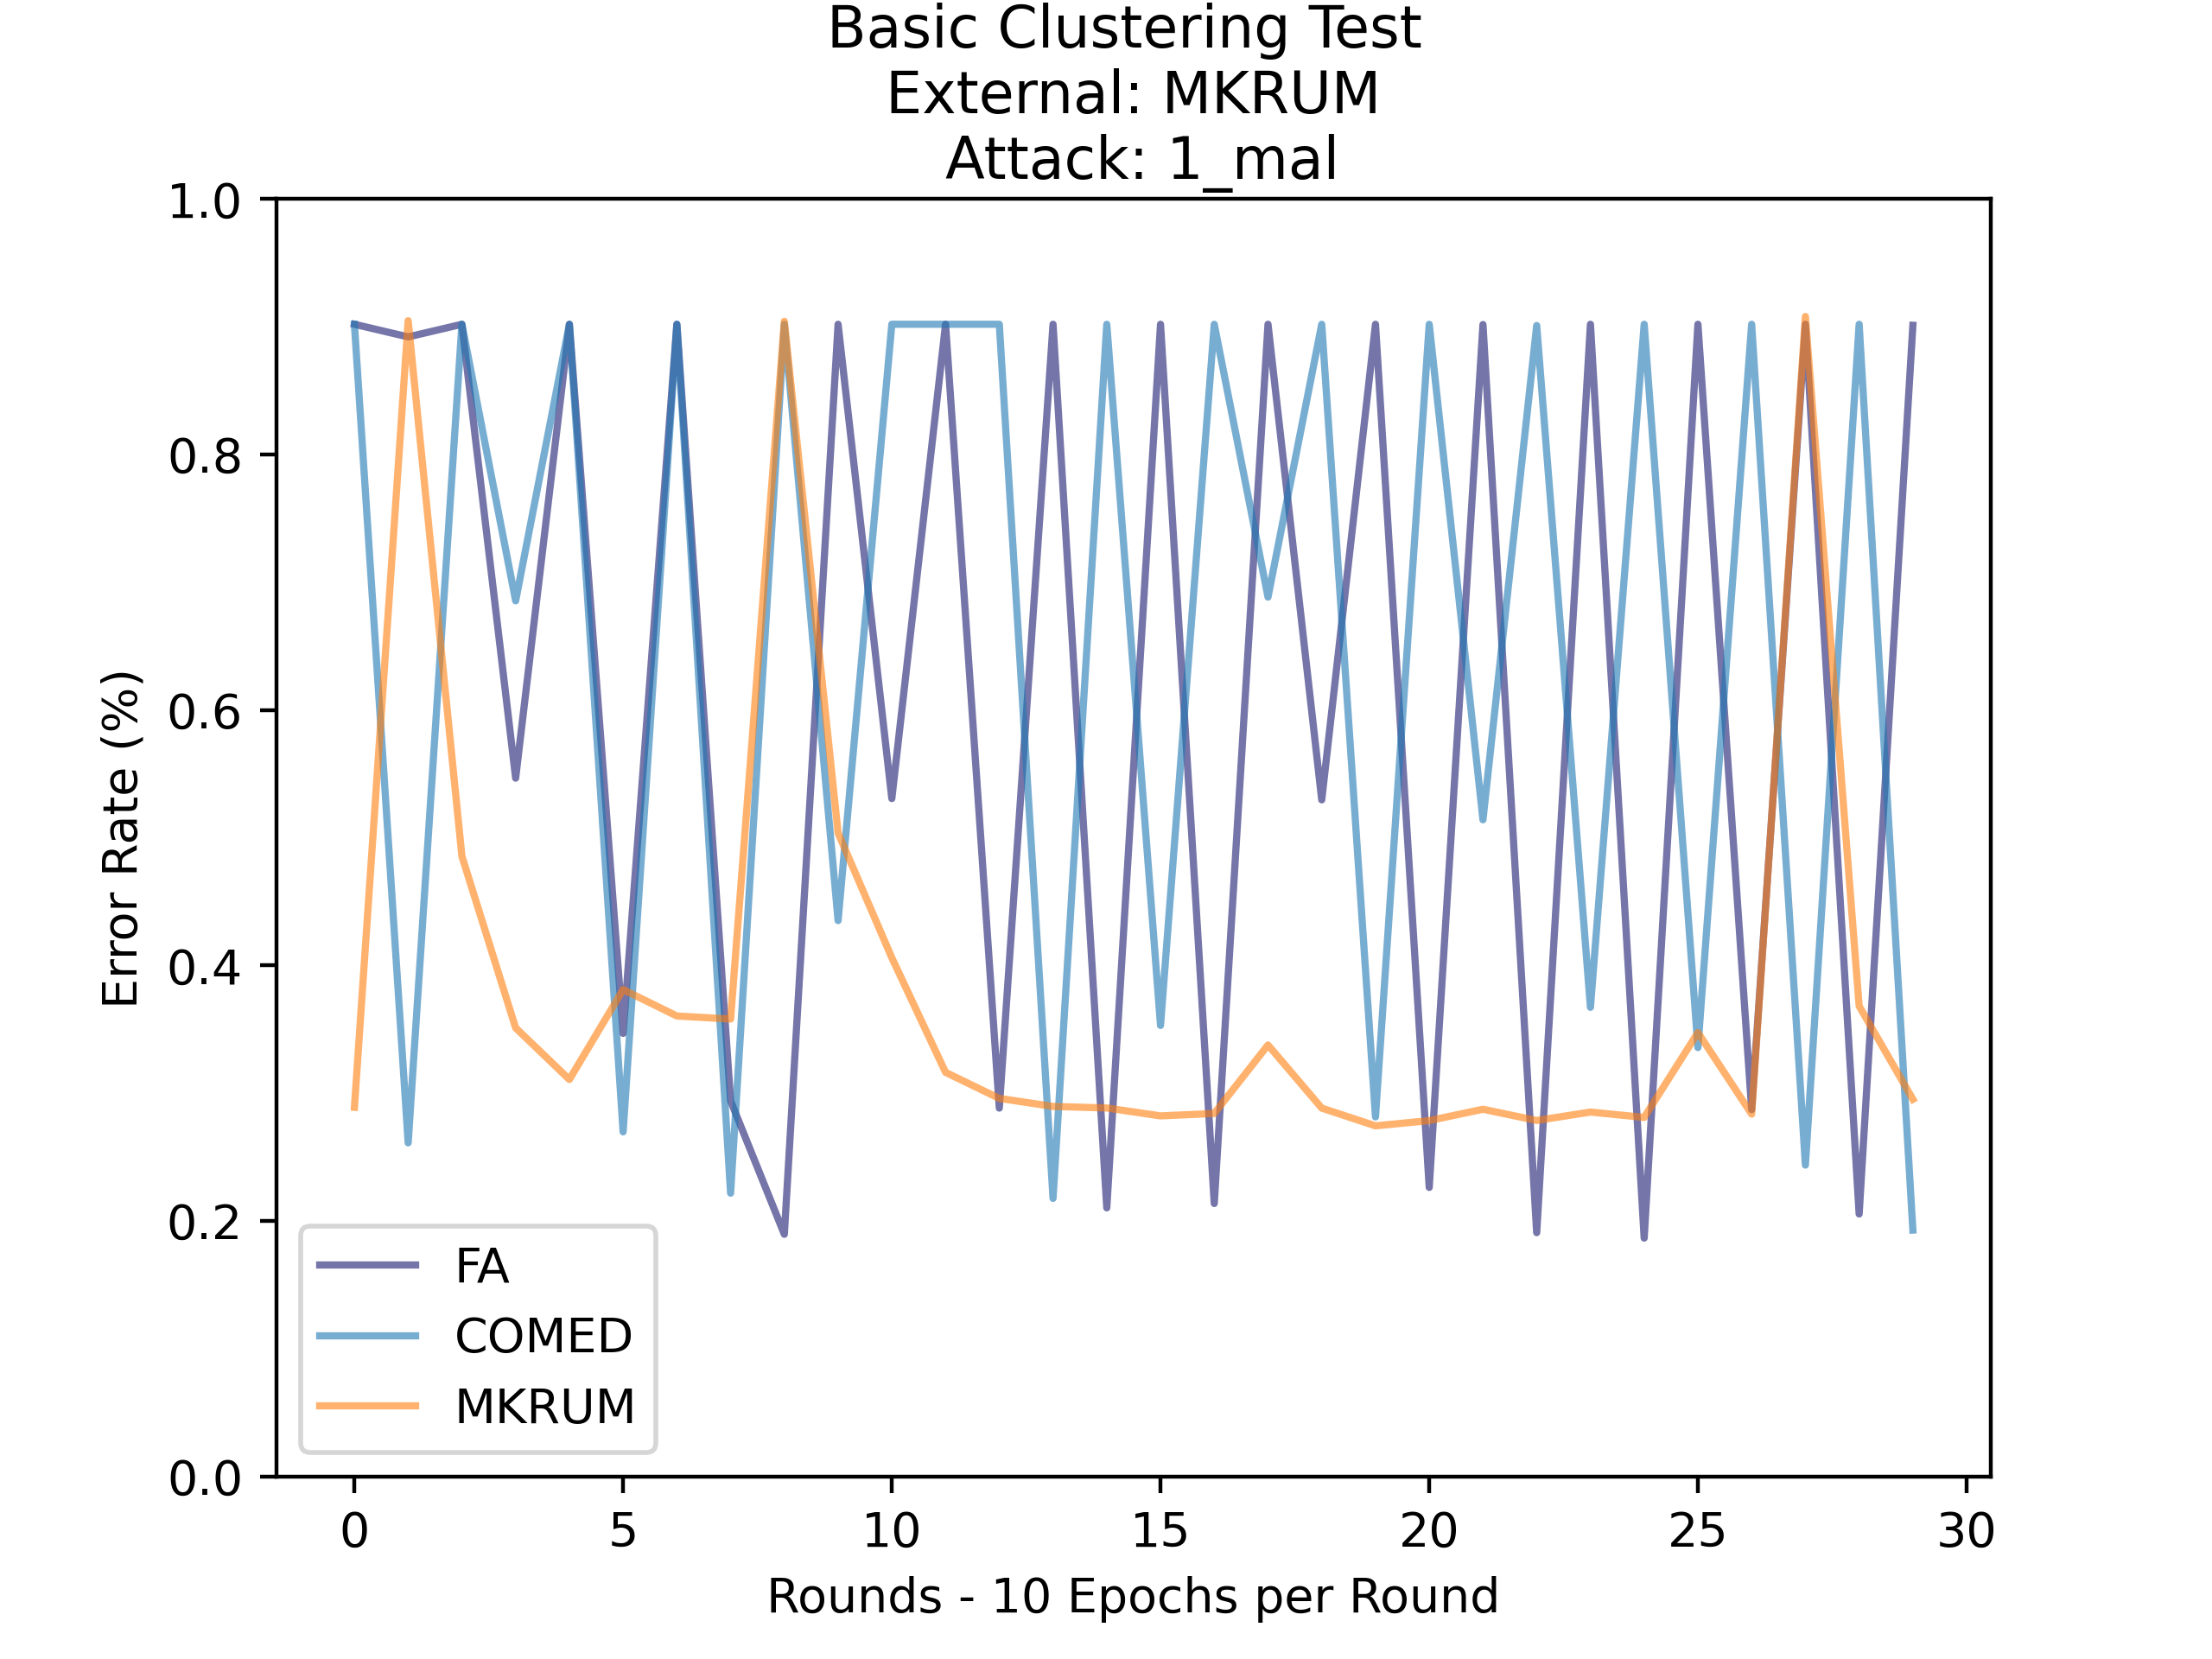
\includegraphics[scale=0.5]{my_agg/graphs/cluster_mkrum_1.png}
	\caption{Error Rate of K-Means Clustering when MKRUM is the External Aggregator}
	\label{fig:mkrum_bad}
\end{figure}

\begin{figure}[htbp]
	\centering
    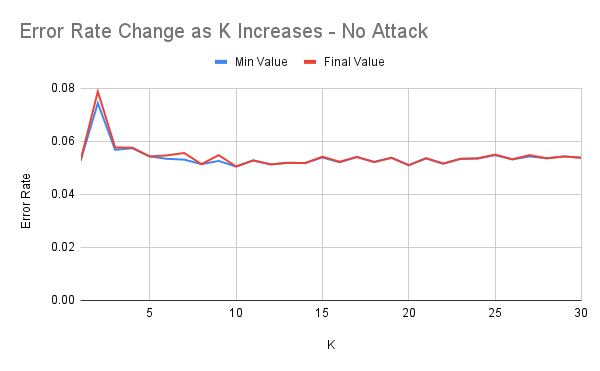
\includegraphics[scale=0.5]{my_agg/graphs/k_elbow_0.png}
	\caption{Error Rate As K Increases - No Attack}
	\label{fig:k_elbow_0}
\end{figure}

\begin{figure}[htbp]
	\centering
    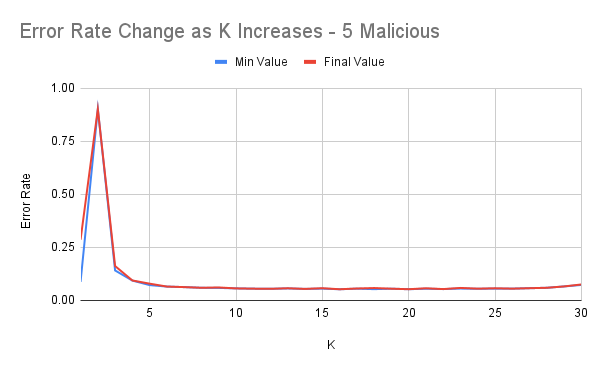
\includegraphics[scale=0.5]{my_agg/graphs/k_elbow_5.png}
	\caption{Error Rate As K Increases - 5 Malicious}
	\label{fig:k_elbow_5}
\end{figure}

\begin{figure}[htbp]
	\centering
    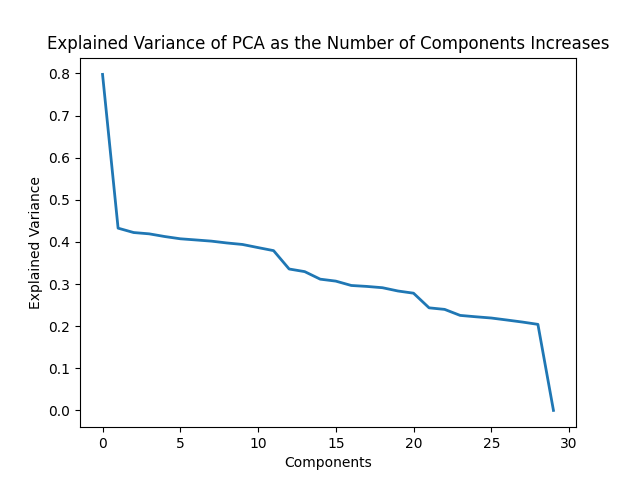
\includegraphics[scale=0.5]{my_agg/graphs/0_r1.png}
	\caption{Explained Variance with No Attacks at Round 1}
	\label{fig:pca_01}
\end{figure}

\begin{figure}[htbp]
	\centering
    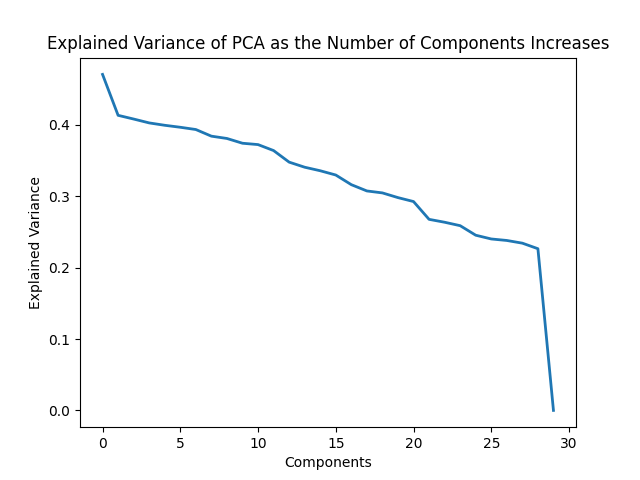
\includegraphics[scale=0.5]{my_agg/graphs/0_r2.png}
	\caption{Explained Variance with No Attacks at Round 2}
	\label{fig:pca_02}
\end{figure}

\begin{figure}[htbp]
	\centering
    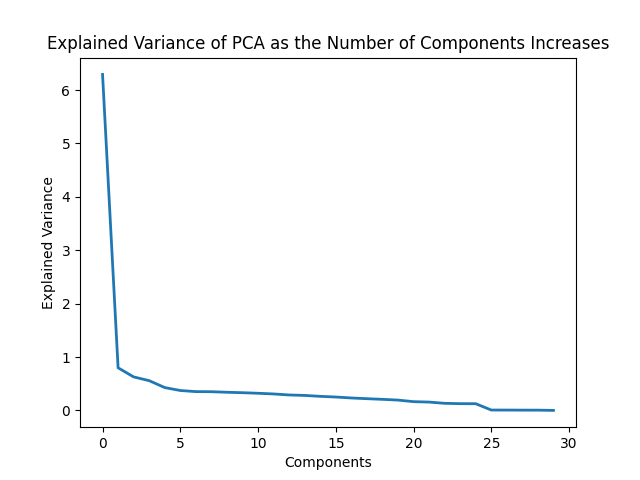
\includegraphics[scale=0.5]{my_agg/graphs/5_r0.png}
	\caption{Explained Variance with 5 Malicious at Round 0}
	\label{fig:pca_50}
\end{figure}

\begin{figure}[htbp]
	\centering
    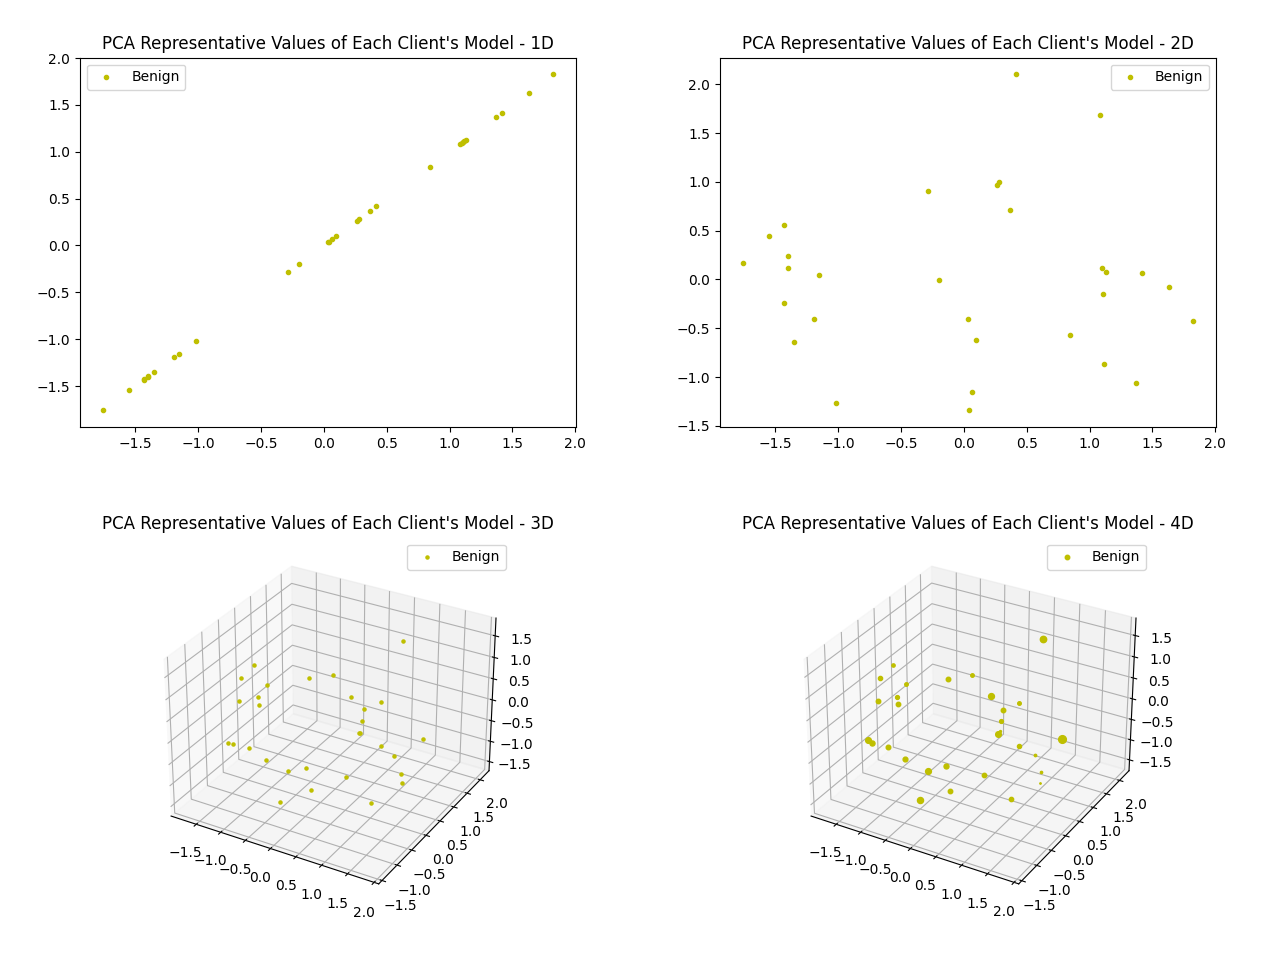
\includegraphics[scale=0.3]{my_agg/graphs/0mal_dims.png}
	\caption{PCA Transform Positions over Four Dimensions - No Attacks - Round 0}
	\label{fig:0mal_dims}
\end{figure}

\begin{figure}[htbp]
	\centering
    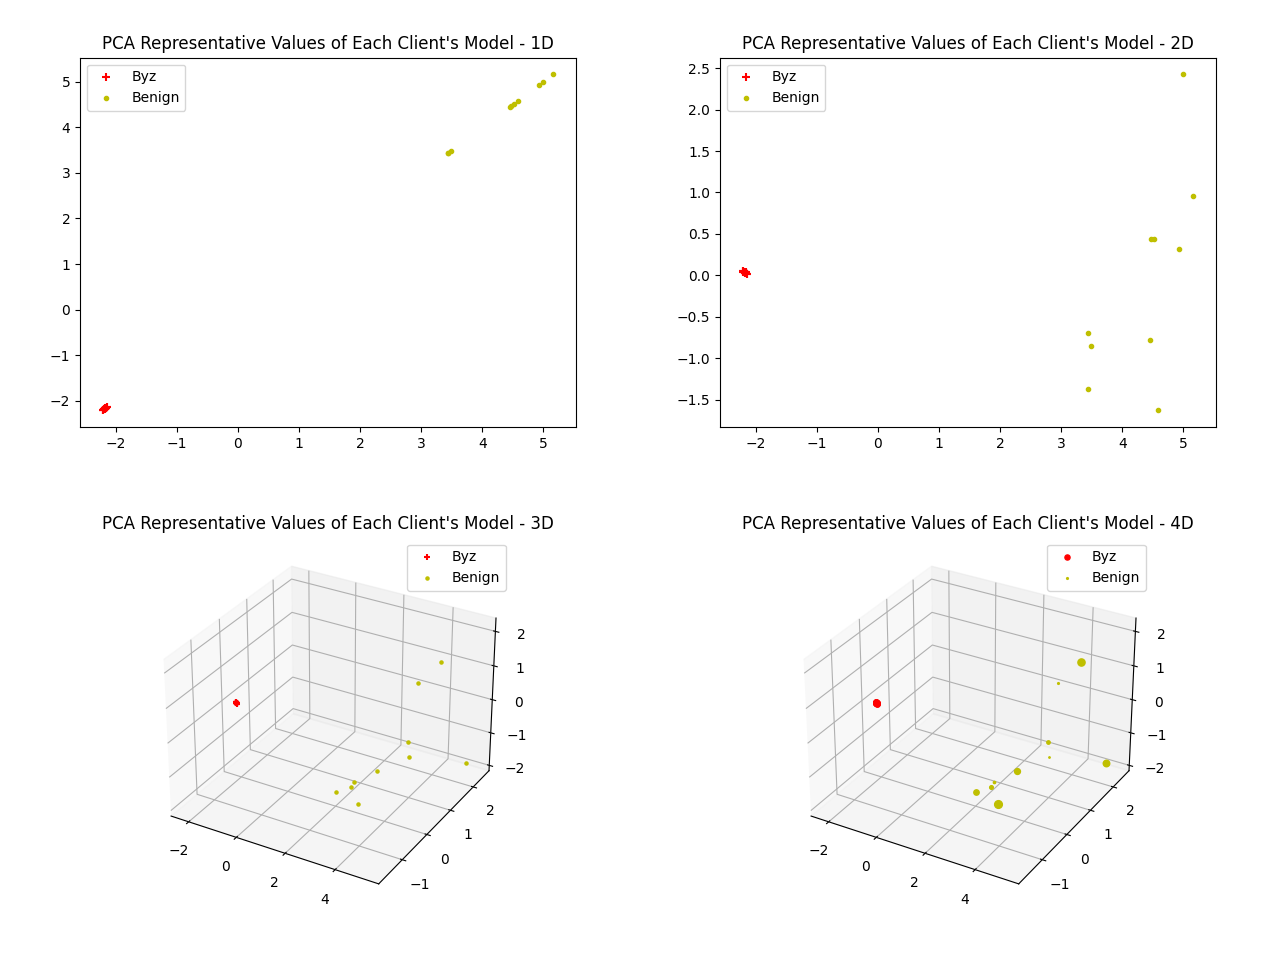
\includegraphics[scale=0.3]{my_agg/graphs/20mal_dims.png}
	\caption{PCA Transform Positions over Four Dimensions - 20 Malicious - Round 0}
	\label{fig:20mal_dims}
\end{figure}

\begin{figure}[htbp]
	\centering
    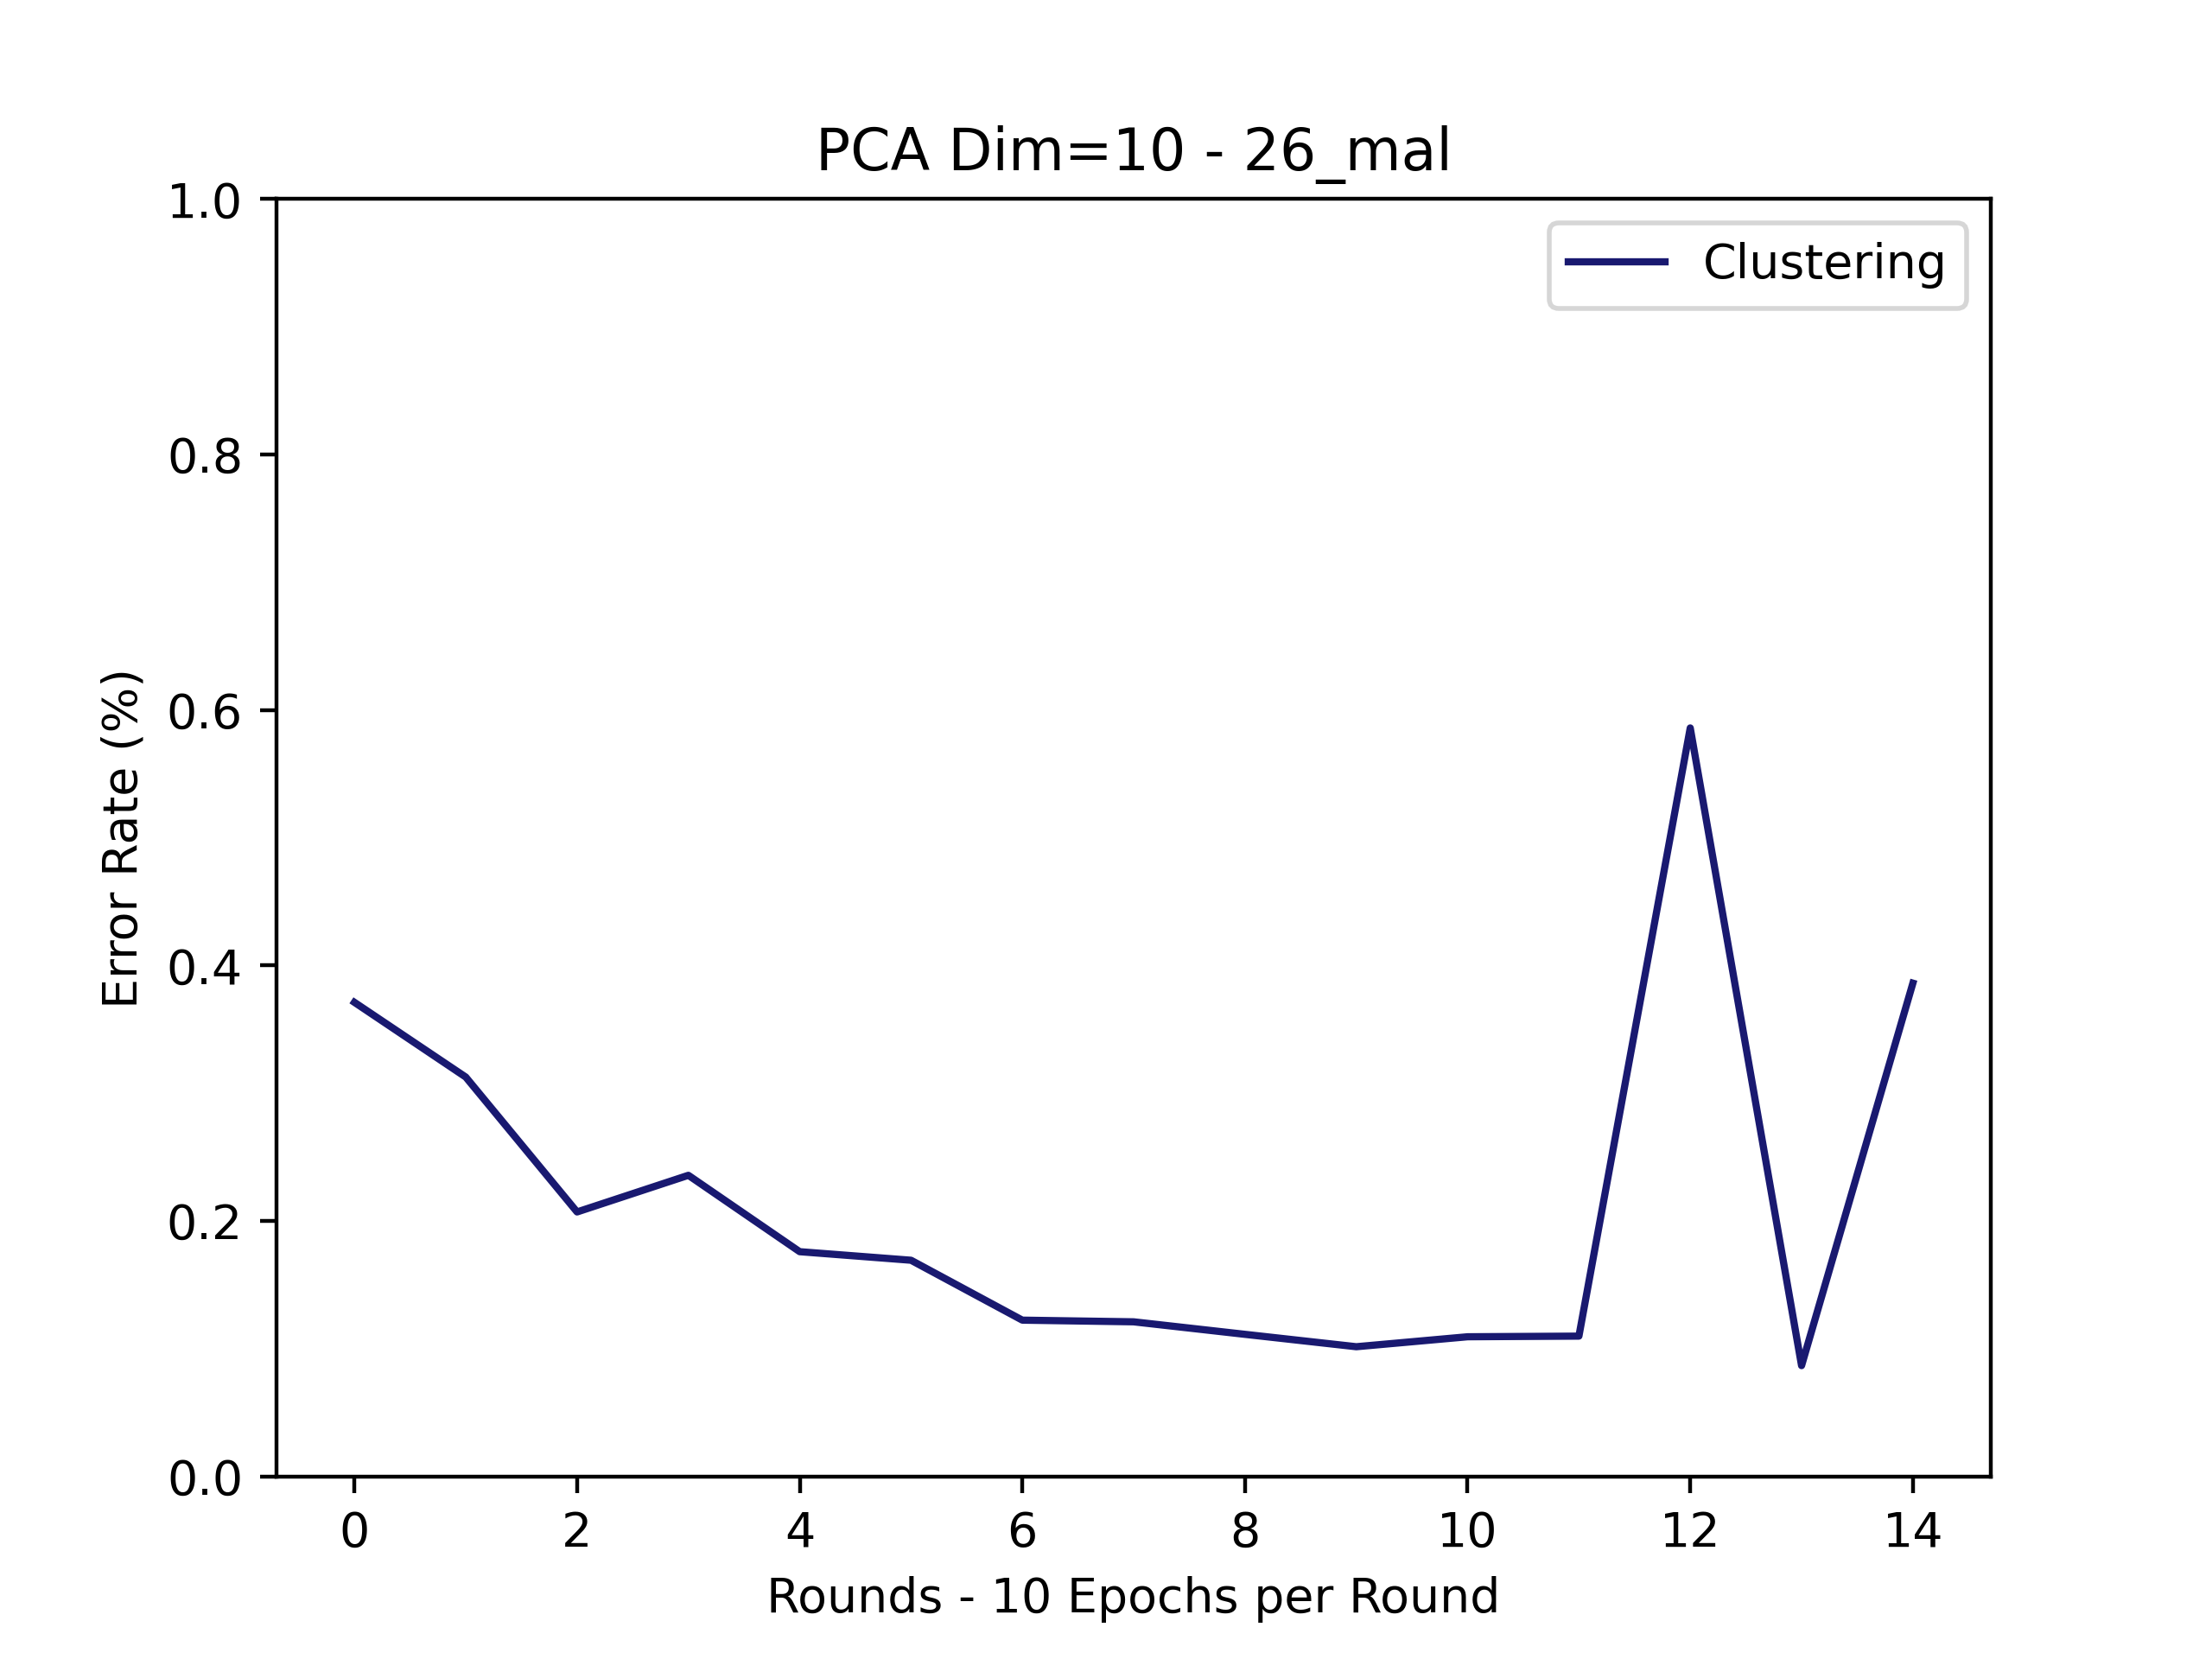
\includegraphics[scale=0.5]{my_agg/graphs/dim10_26mal.png}
	\caption{Less Smooth Performance Exhibited when Dim=10 with 26 Malicious}
	\label{fig:dim10_26mal}
\end{figure}

\begin{figure}[htbp]
	\centering
    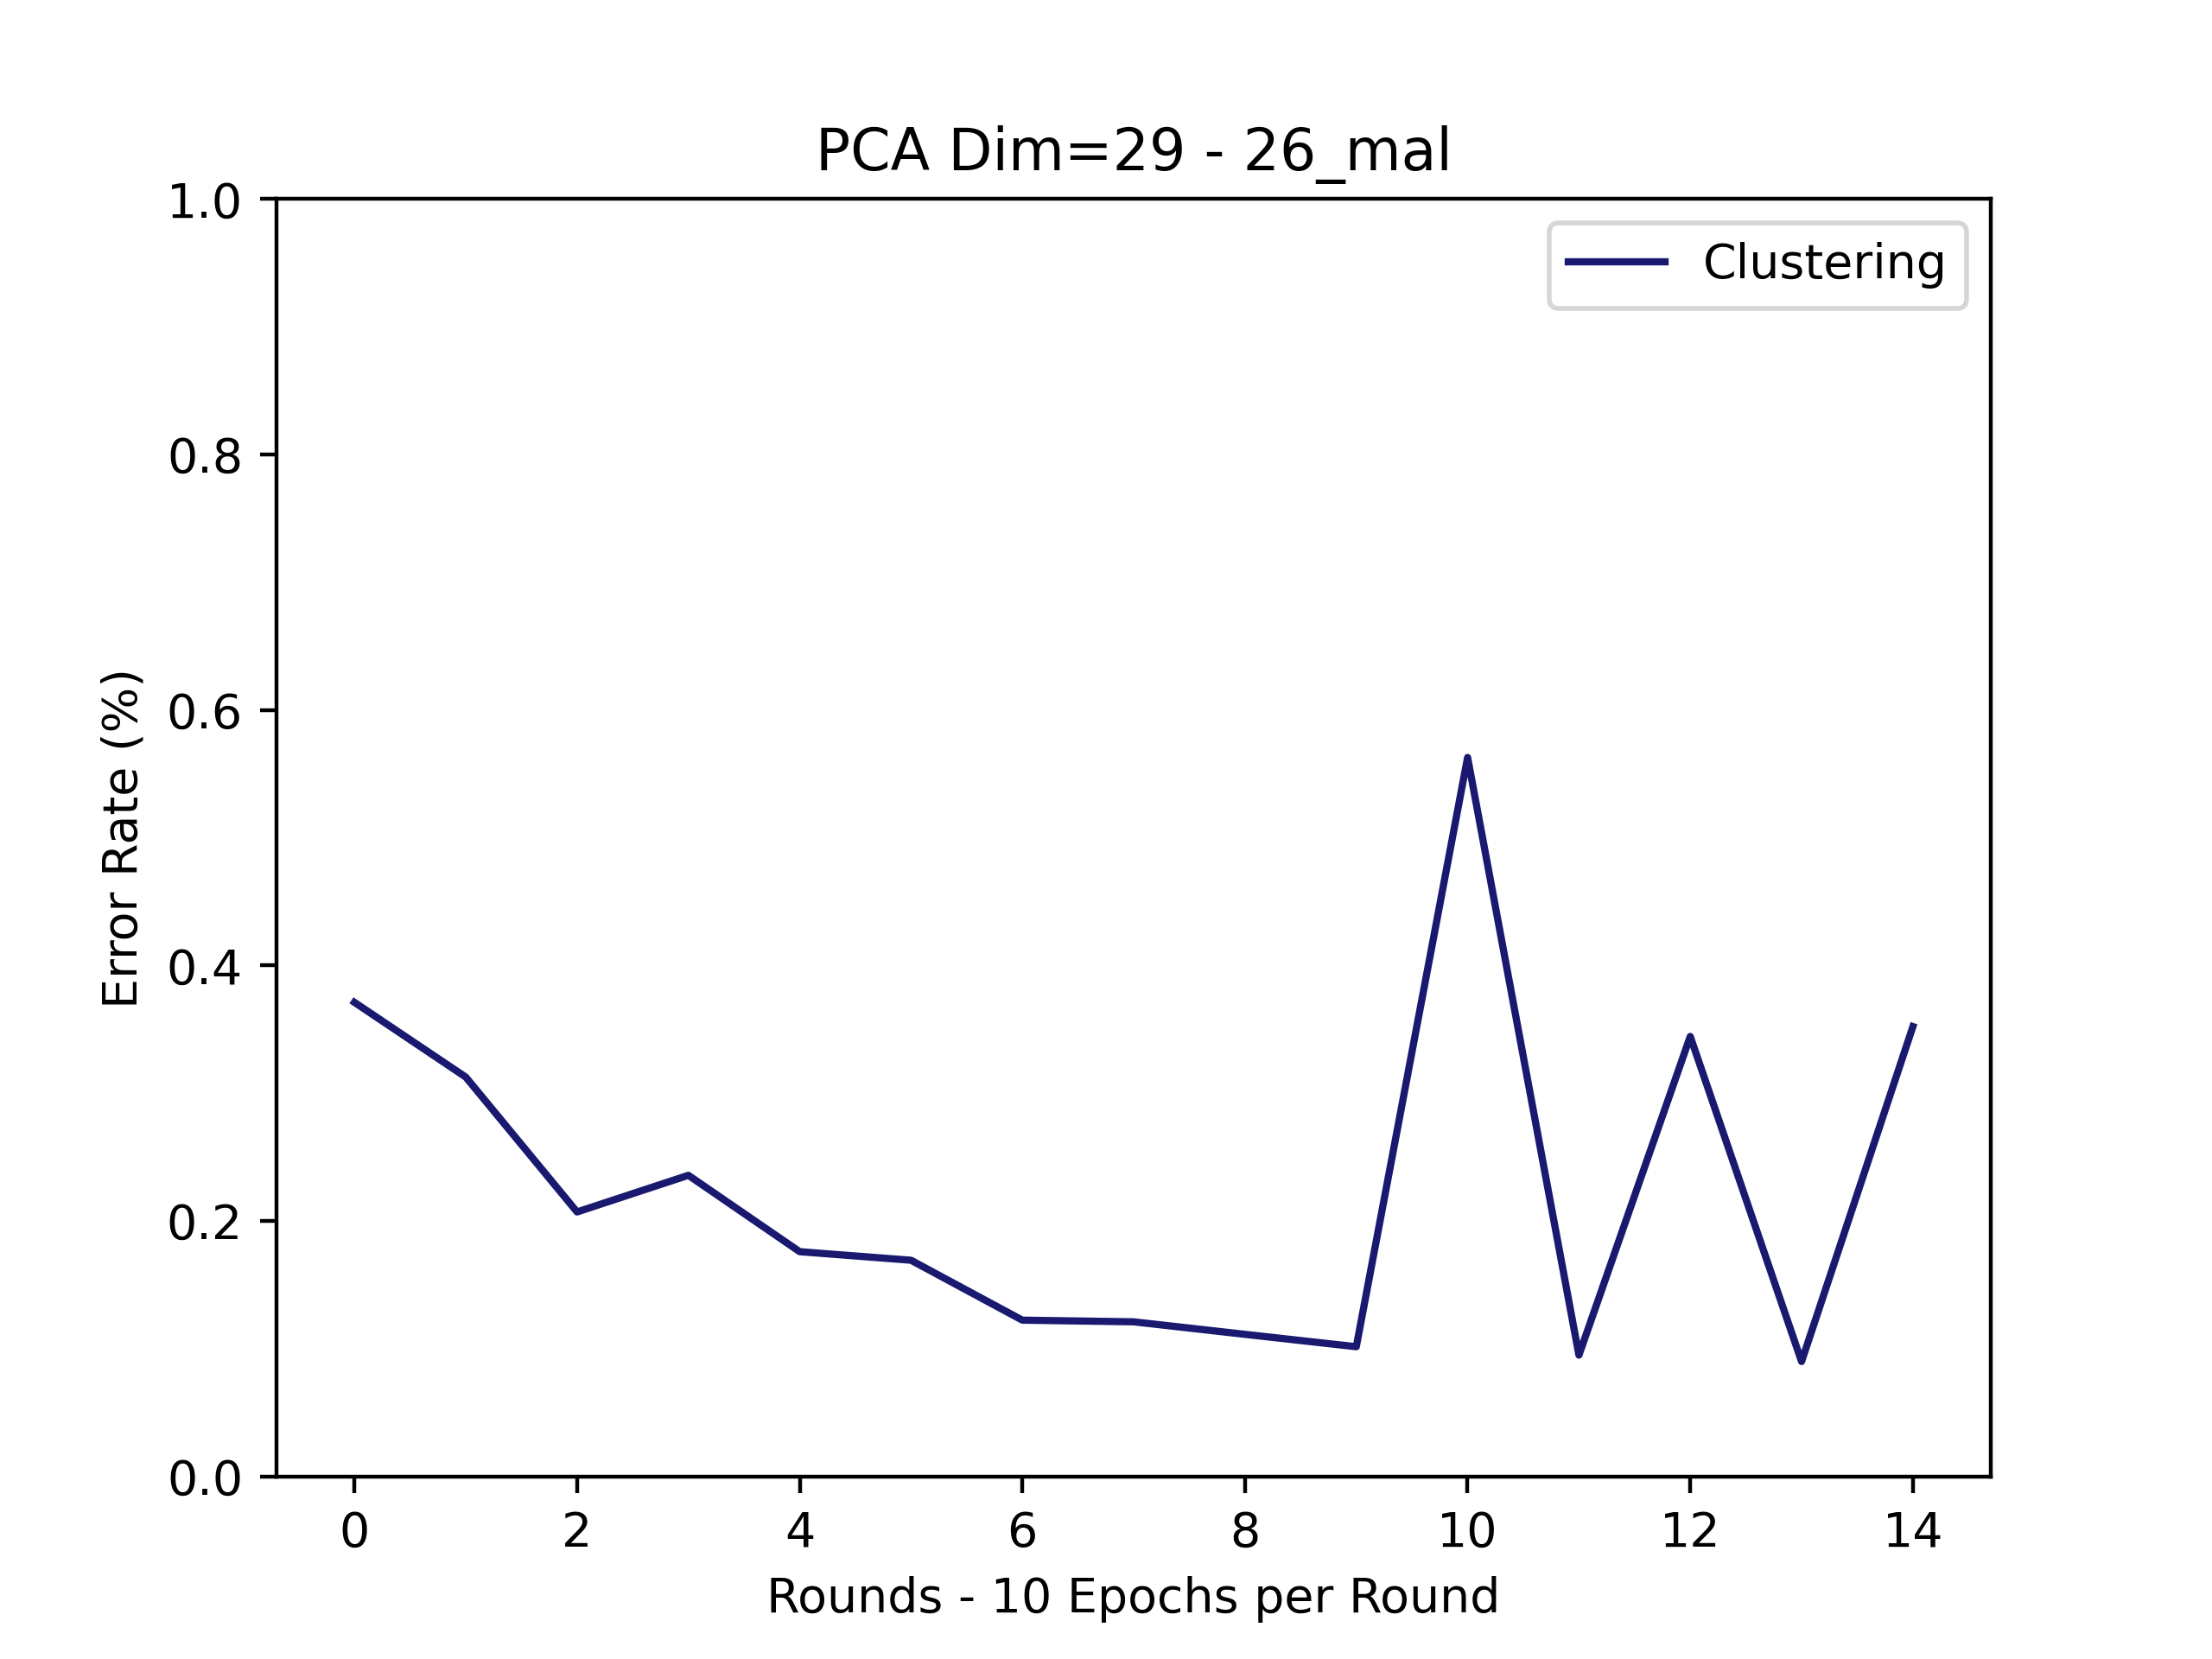
\includegraphics[scale=0.5]{my_agg/graphs/dim29_26mal.png}
	\caption{Less Smooth Performance Exhibited when Dim=29 with 26 Malicious}
	\label{fig:dim29_26mal}
\end{figure}

\begin{figure}[htbp]
	\centering
    \includegraphics[scale=0.5]{my_agg/graphs/comed_4d_24mal.png}
	\caption{4D PCA with COMED as the External Aggregator under various Personalisation Methods - 24 Malicious}
	\label{fig:4d_24mal}
\end{figure}

\begin{figure}[htbp]
	\centering
    \includegraphics[scale=0.5]{my_agg/graphs/fa_4d_5mal.png}
	\caption{4D PCA with FedAvg as the External Aggregator under various Personalisation Methods - 5 Malicious}
	\label{fig:4d_5mal}
\end{figure}

\begin{figure}[htbp]
	\centering
    \includegraphics[scale=0.5]{my_agg/graphs/fa_4d_15mal.png}
	\caption{4D PCA with FedAvg as the External Aggregator under various Personalisation Methods - 15 Malicious}
	\label{fig:4d_15mal}
\end{figure}

\begin{figure}[htbp]
	\centering
    \includegraphics[scale=0.5]{my_agg/graphs/fa_1d_26mal.png}
	\caption{1D PCA with FedAvg as the External Aggregator under various Personalisation Methods - 26 Malicious}
	\label{fig:1d_26mal}
\end{figure}

\begin{figure}[htbp]
	\centering
    \includegraphics[scale=0.5]{my_agg/graphs/1d_no_global.png}
    \caption{4D PCA with the No Global Personalisation Method - 1 Malicious Client}
	\label{fig:4D_no_global_1}
\end{figure}

\begin{figure}[htbp]
	\centering
    \includegraphics[scale=0.5]{my_agg/graphs/no_global_15free.png}
    \caption{4D PCA with the No Global Personalisation Method - 15 Free Clients. This shows Free-Riders not being able to ever learn as they are in the cluster represented by the top line.}
	\label{fig:no_15free}
\end{figure}


\chapter{Project}
\begin{figure}[htbp]
	\centering
    \includegraphics[scale=0.3]{appendices/amir.jpg}
    \caption{Supervisor - Dr Amir Alansary}
    \label{amir}
\end{figure}

\begin{figure}[htbp]
	\centering
    \includegraphics[scale=0.6]{appendices/jon.jpg}
    \caption{Second Marker - Dr Jonathan Passerat-Palmbach}
    \label{jon}
\end{figure}

\begin{figure}[htbp]
	\centering
    \includegraphics[scale=0.18]{appendices/sam.jpg}
    \caption{Author - Samuel Trew}
    \label{sam}
\end{figure}

\end{appendices}


\end{document}